\documentclass[pdftex,a4paper,twoside,11pt]{article}
\NeedsTeXFormat{LaTeX2e}


%% Include layout, additional commands and abbreviations
%%
%% Layout definitions
%%

\usepackage[english]{babel}
\usepackage[T1]{fontenc}
\usepackage[scaled=0.91]{helvet}
\usepackage{sfmath}
\usepackage{amsmath}
\usepackage{fancyhdr}
\usepackage{fancyvrb}
\usepackage[small,bf]{caption}
\usepackage{lastpage}
\usepackage{multirow}
\usepackage{tabularx}
\usepackage{longtable}
\usepackage{graphicx}
\usepackage{url}
\usepackage[usenames,dvipsnames]{color}

\definecolor{darkblue}{rgb}{0,0,0.5}
\definecolor{red}{rgb}{1,0,0}
\definecolor{green}{rgb}{0,1,0}
\definecolor{orange}{rgb}{1,0.5,0}

\usepackage[pdftex,
            colorlinks=true,
            pdfstartview=FitV,
            linkcolor=darkblue,
            citecolor=darkblue,
            urlcolor=blue,
            plainpages=false,
            pdfpagelabels,
            linktocpage,
            backref,
            pagebackref]{hyperref}

\hypersetup{
  pdftitle={METIS Reflex Tutorial},
  pdfauthor={METIS Pipeline Team},
  pdfkeywords={METIS, Data Reduction, Pipeline, Reflex, Tutorial},
  pdfsubject={METIS Reflex Tutorial}
}
\usepackage[public]{dmd-doc}

%%% Local Variables: 
%%% mode: latex
%%% TeX-master: t
%%% End:

%%
%%      UPDATE FOR NEW RELEASES
%%
\newcommand{\releasedate}{June 2022}
\newcommand{\manualversion}{1.5.0}


\newcommand{\cm}[1]{\marginpar{\scriptsize #1}}
\newcommand{\tbspa}{\rule[1ex]{0pt}{1.1ex}}
\newcommand{\tbspb}{\rule[-1.0ex]{0pt}{1.0ex}}
\newcommand{\eg}{{e.g.~}}
\newcommand{\ie}{{i.e.~}}
\newcommand{\degr}{\hbox{$^\circ$}}
\newcommand{\CPL}{\textit{Common Pipeline Library }}
\newcommand{\HDRL}{\textit{High Level Data Reduction Library }}
\newcommand{\http}[1]{\href{http://#1}{\textit{http://#1}}}


\newcommand{\putgraph}[4]{
    \subfigure
    \begin{figure}[ht]
        \begin{center}
    \includegraphics[width=#1truecm]{figures/#2}
    \end{center}
    \caption{\it #4.}
    \label{fig:#3}
    \end{figure}
}

\makeatletter
\newcommand\footnoteref[1]{\protected@xdef\@thefnmark{\ref{#1}}\@footnotemark}
\makeatother
\newcommand{\floor}[1]{\lfloor #1 \rfloor}


\pdmProgram{GEN}
\pdmProject{Science Operation Software Department}
\pdmTitle{HDRL Pipeline Developer Manual}
\pdmDocId{ESO-299492}
\pdmDocVersion{6}
\pdmSoftwareVersion{1.5.0}
\pdmDocType{Manual (MAN)}
\pdmDocDate{\DTMdate{2022-06-01}}
\pdmPreparedBy{}
\pdmValidatedBy{}
\pdmApprovedBy{}

\setlongtables
\makeindex

\bibliographystyle{plain} 

\begin{document}

\definecolor{mygreen}{rgb}{0,0.6,0}
\definecolor{mygray}{rgb}{0.5,0.5,0.5}
\definecolor{mymauve}{rgb}{0.58,0,0.82}
\definecolor{typecol}{rgb}{0.87, 0.36, 0.38}

\lstset{
    language=C,               % choose the language of the code
    backgroundcolor=\color{white},  % choose the background color.
    breakatwhitespace=true, 
    frame=shadowbox,
%    rulesepcolor=\color{blue},
    basicstyle=\ttfamily,
%    stringstyle=\color{red}\ttfamily,
    stringstyle=\color{mymauve}\ttfamily,
    commentstyle=\color{mygreen}\ttfamily,
    keywordstyle=\color{typecol}\ttfamily,
    morekeywords={*, hdrl_value, hdrl_image, hdrl_imagelist, hdrl_parameter,
      hdrl_direction, hdrl_bpm_3d_method, hdrl_mode_type, hdrl_image_extend_method},
    morekeywords={*, hdrl_overscan_compute_result, hdrl_overscan_correct_result},
    morekeywords={*, hdrl_strehl_result, hdrl_catalogue_result,
      hdrl_catalogue_options, hdrl_resample_result},
    morekeywords={*, hdrl_bitmask_t, HDRL_ITER_OWN_OUTPUT, size_t, hdrl_iter,
        hdrl_buffer},
    morekeywords={*, hdrl_spectrum1D, hdrl_spectrum1D_wavelength, hdrl_spectrum1D_interp_akima, hdrl_response_result},
    morekeywords={*, cpl_image, cpl_table, cpl_mask, cpl_imagelist, cpl_size,
      cpl_parameterlist, cpl_propertylist,
        cpl_parameter, cpl_error_code, cpl_filter_mode, cpl_wcs,
        cpl_border_mode, cpl_vector, cpl_boolean},
    keywordstyle=[2]{\color{blue}\ttfamily},
    morekeywords=[2]{hdrl_overscan_compute, hdrl_overscan_parameter_create,
        hdrl_collapse_mean_parameter_create,
        hdrl_collapse_median_parameter_create,
        hdrl_collapse_weighted_mean_parameter_create,
        hdrl_collapse_sigclip_parameter_create,
        hdrl_collapse_minmax_parameter_create,
        hdrl_collapse_mode_parameter_create,
        hdrl_rect_region_parameter_create,
        hdrl_overscan_compute_result_get_correction,
        hdrl_overscan_compute_result_get_contribution,
        hdrl_overscan_compute_result_get_chi2,
        hdrl_overscan_compute_result_get_red_chi2,
        hdrl_overscan_compute_result_get_sigclip_reject_low,
        hdrl_overscan_compute_result_get_sigclip_reject_high,
        hdrl_overscan_compute_result_get_minmax_reject_low,
        hdrl_overscan_compute_result_get_minmax_reject_high,
        hdrl_overscan_compute_result_delete,
        hdrl_overscan_correct,
        hdrl_overscan_compute,
        hdrl_overscan_correct_result_get_corrected,
        hdrl_overscan_correct_result_unset_corrected,
        hdrl_overscan_correct_result_get_badmask,
        hdrl_overscan_correct_result_delete,
        hdrl_overscan_parameter_create_parlist,
        hdrl_overscan_parameter_parse_parlist,
        hdrl_catalogue_parameter_create_parlist,
        hdrl_catalogue_parameter_parse_parlist,
        hdrl_catalogue_result_delete,
        hdrl_spectrum1D_resample_interpolate_parameter_create,
        hdrl_efficiency_compute,
        hdrl_spectrum1D_get_wavelength,
        hdrl_spectrum1D_resample,
        hdrl_spectrum1D_mul_scalar,
        hdrl_spectrum1D_mul_scalar_create,
        hdrl_spectrum1D_convert_to_table,
        hdrl_efficiency_parameter_create,
        hdrl_response_compute,
        hdrl_response_telluric_evaluation_parameter_create, 
        hdrl_spectrum1D_shift_fit_parameter_create,
        hdrl_response_parameter_create,
        hdrl_response_fit_parameter_create,
        hdrl_response_result_delete
    },
    morekeywords=[2]{hdrl_parameter_destroy, hdrl_parameter_delete},
    morekeywords=[2]{hdrl_imagelist_collapse_mean,
        hdrl_imagelist_collapse_median,
        hdrl_imagelist_collapse_weighted_mean,
        hdrl_imagelist_collapse_sigclip,
        hdrl_imagelist_collapse_minmax,
        hdrl_imagelist_collapse_mode,
        hdrl_imagelist_collapse,
        hdrl_imagelist_new,
        hdrl_imagelist_set,
        hdrl_imagelist_sub_image,
        hdrl_collapse_parameter_create_parlist,
        hdrl_collapse_parameter_parse_parlist,
        hdrl_collapse_parameter_is_mean,
        hdrl_collapse_parameter_is_median,
        hdrl_collapse_parameter_is_weighted_mean,
        hdrl_collapse_parameter_is_sigclip,
        hdrl_collapse_sigclip_parameter_get_kappa_low,
        hdrl_collapse_sigclip_parameter_get_kappa_high,
        hdrl_collapse_sigclip_parameter_get_niter
    },
    morekeywords=[2]{hdrl_imagelist_add_scalar,hdrl_imagelist_mul_scalar,
        hdrl_imagelist_row_view,
        hdrl_imagelist_create,
        hdrl_imagelist_delete,
        hdrl_imagelist_get_iter_row_slices,
    },
    morekeywords=[2]{hdrl_image_create, hdrl_image_duplicate,
        hdrl_image_add_scalar,
        hdrl_image_add_image,
        hdrl_image_mul_scalar,
        hdrl_image_sub_image,
        hdrl_image_div_scalar,
        hdrl_image_reject,
        hdrl_image_delete,
        hdrl_iter_next,
        hdrl_iter_delete,
        process,
        process_big_data,
    },
    morekeywords=[2]{hdrl_spectrum1D_delete,
    },
    morekeywords=[2]{
        hdrl_buffer_allocate,
        hdrl_buffer_free,
        hdrl_buffer_delete,
        hdrl_buffer_new,
        hdrl_image_new_from_buffer,
    },
    morekeywords=[2]{cpl_parameterlist_get_first, cpl_parameterlist_get_next,
        cpl_parameterlist_append,
        cpl_parameterlist_delete,
        cpl_parameterlist_disable,
    },
    morekeywords=[2]{hdrl_bpm_2d_compute, hdrl_bpm_3d_compute,
      hdrl_bpm_fit_compute, hdrl_lacosmic_edgedetect,
       hdrl_bpm_2d_parameter_create_filtersmooth,
       hdrl_bpm_2d_parameter_create_legendresmooth,
       hdrl_bpm_3d_parameter_create,
       hdrl_bpm_fit_parameter_create_pval,
       hdrl_bpm_fit_parameter_create_rel_chi,
       hdrl_bpm_fit_parameter_create_rel_coef,
       hdrl_lacosmic_parameter_create,   
    },
    morekeywords=[2]{hdrl_fringe_compute, hdrl_fringe_correct,   
    },
    morekeywords=[2]{hdrl_flat_compute, hdrl_flat_parameter_create,
    },
    morekeywords=[2]{hdrl_catalogue_compute, hdrl_catalogue_parameter_create,
    },
    morekeywords=[2]{hdrl_strehl_compute, hdrl_strehl_parameter_create,
    },
    morekeywords=[2]{hdrl_fpn_compute,
    },
    morekeywords=[2]{hdrl_resample_imagelist_to_table,
      hdrl_resample_image_to_table,
      hdrl_resample_compute,
      hdrl_resample_result_delete,
      hdrl_resample_parameter_create_outgrid2D,
      hdrl_resample_parameter_create_outgrid3D,
      hdrl_resample_parameter_create_outgrid2D_userdef,
      hdrl_resample_parameter_create_outgrid3D_userdef,
      hdrl_resample_parameter_create_renka,
      hdrl_resample_parameter_create_drizzle,
      hdrl_resample_parameter_create_nearest,
      hdrl_resample_parameter_create_linear,
      hdrl_resample_parameter_create_quadratic,
      hdrl_resample_parameter_create_lanczos
    },
    morekeywords=[2]{hdrl_download_url_to_buffer,
      hdrl_download_url_to_file,
      hdrl_barycorr_compute,
      hdrl_eop_data_totable
    },
    morekeywords=[2]{hdrl_maglim_compute,
    }
}

\pagenumbering{arabic}
\pdmmaketitle

\begin{center}
  \textbf{\Large Authors}
  
\begin{tabularx}{\linewidth}{|p{0.25\linewidth}|X|}
  \hline
  \multicolumn{1}{|l|}{\textbf{Name}}\tbspa &
  \multicolumn{1}{l|}{\textbf{Affiliation}} \tbspb \\
  \hline
  \tbspa
  The HDRL Team & ESO \tbspb\\
  \hline
\end{tabularx}
\end{center}

\begin{center}
  \textbf{\Large Change record}

  \tablehead{\hline
    \multicolumn{1}{|c|}{Issue/Rev.}\tbspa &
    \multicolumn{1}{|c|}{Date} &
    \multicolumn{1}{|c|}{Section/Parag.\ affected} &
    \multicolumn{1}{|c|}{Reason/Initiation/Documents/Remarks}\tbspb \\
    \hline}
  \tabletail{\hline}

  \begin{supertabular}{|l|l|l|l|}
    0.0.1\tbspa   & 26/04/2013 & All & Overscan Computation \& Correction \\
    0.0.2\tbspa   & 09/08/2013 & All & Master Bias \& Master Dark \\
    0.0.3\tbspa   & 29/11/2013 & All & First Release \\
    0.1.0\tbspa   & 17/09/2014 & \ref{sec:bpm:main} & Bad Pixel Detection \\
    0.1.5\tbspa   & 15/12/2014 & All & Clipping Algorithm: IQR $\rightarrow$ MAD, Library Integration \\
    0.2.0\tbspa   & 01/05/2015 & \ref{flat:main}, \ref{strehl:main} & Master Flatfield, Strehl Ratio \\
    0.3.0b1\tbspa & 26/11/2015 & \ref{flat:main}, \ref{fringe:main} & Master Flatfield, Master Fringe \\
    1.0.0\tbspa   & 01/04/2017 & \ref{catalogue:main} & Object catalogue generation \\
    1.1.0\tbspa   & 01/04/2018 & \ref{strehl:main}, \ref{efficiency:main}, \ref{response:main} & Strehl Ratio, Spectral Efficiency, Spectral Response,\\
                  &            & \ref{refraction:main} and \ref{chap:DAR}, \ref{airmass:main} & Differential Atmospheric Refraction, Effective air mass \\
    1.2.0\tbspa   & 01/10/2018 & \ref{patternnoise:main}, \ref{sec:algorithms:strehl:example}, \ref{efficiency:main} & Fixed Pattern Noise, Strehl Ratio, Spectral Efficiency\\
    1.3.0\tbspa   & 12/02/2021 & \ref{resampling:main} and \ref{chap:assessing:resampling} & Resampling and Assessment of 2D images and 3D cubes \\
    1.4.0\tbspa   & 30/09/2021 & \ref{sec:algorithms:maglim:main}, \ref{chap:algorithms:maglim}, and \ref{sec:algorithms:robust_mean:mode} & Limiting magnitude and distribution mode \\
    1.5.0\tbspa   & 01/06/2022 & \ref{sec:algorithms:barycorr:main}, \ref{SoftwareInfrastructure:Releases}, and \ref{library_dependencies} & Barycentric correction and library dependencies \\

  \end{supertabular}
\end{center}

\clearpage

{\small
\tableofcontents
%\cleardoublepage
}
\begingroup
\let\cleardoublepage\relax
\let\clearpage\relax

\section{Introduction}

\subsection{Motivation and Purpose}

The ESO Pipeline System Group (PPS) is developing and maintaining
a large variety of data reduction pipelines for the different
instruments. In order to decrease the implementation and maintenance
efforts of the single pipelines the \HDRL projects was launched. 

The \HDRL project aims to identify and concentrate cross-pipeline
algorithms in a single place, verify and homogenize algorithms,
implement error propagation and extensively test the different
functionality. Moreover, this should not only accelerate the
development of new pipelines, but all pipelines would instantaneously
benefit from bug-fixes and improvements in \HDRL.


The various consortia are also encouraged to propose new
functionality/algorithms for the library - the PPS and SDP department
will then evaluate the algorithm and decide if they should be part of
the \HDRL.

The pipeline developer but also the consortia are highly encouraged to
use the new library - if for some reason they want to implement
another solution to an already existing algorithm they should inform
PPS.



\subsection{Stakeholders}

The following actors may interact with the \HDRL project:
SciOps, SDP, USD, QC, PPS, Consortia

%\subsection{Acknowledgements}

\subsection{Scope and references}

The modules implemented in the \HDRL are high-level functionalities that
are intended to be used by several VLT/VLTI instrument pipelines.

The \CPL plays exactly this role for low-level functionalities. 
\bibliography{hdrlpdoc}
\endgroup

\section{Software Infrastructure}

\subsection{SVN usage and library integration}
\label{library_integration}

Th \HDRL library should be included into the pipeline library during
the svn checkout by using the svn::external concept. The external
should point to a given library release in the tags and not to the
trunk, i.e. to a sub-directory of
\verb,http://svnhq2.hq.eso.org/p2/tags/Pipelines/common/hdrl, (see
also sect.~\ref{SoftwareInfrastructure:Releases}). In order to build
the library one has to add the \textit{hdrl.m4} from the common
\textit{m4macros} repository (\verb,Pipelines/common/m4macros, in SVN) to the
pipeline sources.
Then one has to modify the \textit{configure.ac} and the top-level
\textit{Makefile.am} as follows:
\begin{itemize}
\item \textit{configure.ac}: 
\begin{verbatim}
# mark hdrl folder as containing a configurable package
AC_CONFIG_SUBDIRS([hdrl])

# check and define all required variables to build and
# link hdrl external located in the hdrl folder
HDRL_CHECK([hdrl])
\end{verbatim}
\item \textit{Makefile.am}:
\begin{verbatim}
SUBDIRS = hdrl ...
\end{verbatim}
\end{itemize}
Moreover, the variable
\verb,$(HDRL_LIBS), must also be added to the link variable,
\verb,$(HDRL_LDFLAGS), to the linker flag variable, and
\verb,$(HDRL_INCLUDES), to the \verb,AM_CPPFLAGS, variable in the
\textit{Makefile.am} of any folder making use of HDRL. As HDRL is
currently a static library it also needs has to be added as a
dependency of objects using it so these are relinked when HDRL
changes. For example:

\begin{verbatim}
hdrldemo_bias_la_LDFLAGS = $(HDRL_LDFLAGS) ...
hdrldemo_bias_la_LIBADD = $(HDRL_LIBS) ...
hdrldemo_bias_la_DEPENDENCY = $(LIBHDRL) ...
\end{verbatim}

In the source files, the only include needed is:

\begin{lstlisting}
#include <hdrl.h>
\end{lstlisting}



\begingroup
\let\cleardoublepage\relax
\let\clearpage\relax

\subsection{Releases}
\label{SoftwareInfrastructure:Releases}

There is no fixed release cycle for the \HDRL library (as e.g. for
CPL), but new releases are feature-driven, i.e. if there are new
functionality/algorithms available and carefully tested a new
release will be announced and the pipeline developer can change the
svn::external to this new release. This has the advantage that the
pipeline developer has more freedom to decide when to update the
pipeline. On the other hand it allows the developer to incorporate the
new \HDRL release to his pipeline on a very short timescale and
prepare a new Paranal/public release. This is only possible as the
library is not installed in the Data Flow System environment in
Paranal (like CPL) but delivered inside each pipeline.

\subsubsection{Release version 1.5.0}
The \HDRL release version 1.5.0 can be included from\\

http://svnhq2.hq.eso.org/p2/tags/Pipelines/common/hdrl/hdrl-1.5.0

In this release we updated and/or added the following algorithms:
\begin{itemize}
\item The computation of the barycenric correction, i.e. the
  wavelength shift to apply to a spectrum to compensate for the motion
  of the observer with respect to the barycenter of the solar system.
  The implemented algorithm derives the barycentric correction of an
  observation by using the
  \href{https://github.com/liberfa/erfa}{ERFA} (Essential Routines for
  Fundamental Astronomy) library. ERFA is a C library containing key
  algorithms for astronomy, and is based on the
  \href{http://www.iausofa.org}{SOFA library} published by the
  International Astronomical Union (IAU).  See
  section~\ref{sec:algorithms:barycorr:main} for detailed information.
\item The build system has been modified to include GSL as direct
   dependency to the hdrl unit-test as direct GSL calls are performed
   when unit-testing the limiting magnitude module.
 \item For the barycentric correction algorithm two additional
   dependencies were added to the \HDRL.
   \begin{itemize}
     \item A dependency to the
       \href{https://github.com/liberfa/erfa}{ERFA} (Essential
       Routines for Fundamental Astronomy) library
     \item A dependency to the
       \href{https://curl.se/libcurl/}{libcurl} (The multiprotocol
       file transfer library) library
   \end{itemize}  
\end{itemize}

\subsubsection{Release version 1.4.0}
The \HDRL release version 1.4.0 can be included from\\

http://svnhq2.hq.eso.org/p2/tags/Pipelines/common/hdrl/hdrl-1.4.0

In this release we updated and/or added the following algorithms:
\begin{itemize}
\item The computation of the limiting magnitude of an image as defined
  in the \textit{ESO Phase 3 Standard}. The limiting magnitude
  characterizes the depth of an observation and is defined as the
  magnitude of a unresolved source whose flux is 5 times the noise
  background, i.e. the magnitude of a point like source detected with
  $\frac{S}{N}=5$. See section~\ref{sec:algorithms:maglim:main} and
  appendix~\ref{chap:algorithms:maglim} for detailed information.
\item To the statistical estimators we added the \textbf{mode} of a
  distribution, i.e. the following algorithms are now supported for
  collapsing imagelists or deriving statistics on images:
  \begin{itemize}
  \item Mean
  \item Weighted mean
  \item min-max rejected mean
  \item $\kappa\sigma$~clipped mean
  \item Median
  \item Mode
  \end{itemize}
  Please note that all methods but the mode are doing \textbf{error
    propagation}. The mode method is special in this case as it
  \textbf{calculates the error from the data}. The error estimation
  can either be done analytically or based on a bootstrap Montecarlo
  simulation. In this case the input data are perturbed with the
  bootstrap technique and the mode is calculated N times (controlled
  with a parameter). From this N modes the standard deviation is
  calculated and returned as error. See
  section~\ref{sec:algorithms:robust_mean:mode} for detailed
  information on the mode algorithm.
\item Due to the addition of the mode, the
  functions\\ \verb+ hdrl_overscan_parameter_create_parlist()+
  and\\ \verb+hdrl_collapse_parameter_create_parlist()+ have
  changed. The two functions now require an additional default mode
  hdrl parameter. See the doxygen information and
  e.g. section~\ref{sec:algorithms:overscan:parameters} and
  section~\ref{sec:algorithms:bias:parameters} for more details.
\end{itemize}


\subsubsection{Release version 1.3.0}
The \HDRL release version 1.3.0 can be included from\\

http://svnhq2.hq.eso.org/p2/tags/Pipelines/common/hdrl/hdrl-1.3.0

In this release we updated and/or added the following algorithms:
\begin{itemize}
\item Resampling of 2-dimensional images and 3-dimensional cubes. A common
  problem in astronomy is the resampling of images (or cubes) onto a common
  grid. Ideally, this is done only once in the data reduction workflow as each
  sub pixel resampling redistributes the flux and leads to correlations. The
  algorithm provided by the \HDRL is doing the 2D and 3D interpolation in
  2-dimensional and 3-dimensional spaces, respectively. Currently there are six
  different interpolation methods implemented:
\begin{center}
\begin{itemize}
\item {\bf Nearest:} Nearest neighbour resampling
\item {\bf Linear:} Weighted resampling using an inverse distance weighting
  function
\item {\bf Quadratic:} Weighted resampling using a quadratic inverse distance
  weighting function
\item {\bf Renka:} Weighted resampling using a Renka weighting function
\item {\bf Drizzle:} Weighted resampling using a drizzle-like weighting scheme
\item {\bf Lanczos:} Weighted resampling using a lanczos-like restricted sinc as
  weighting function
\end{itemize}
\end{center}
  See section~\ref{resampling:main} and appendix~\ref{chap:assessing:resampling}
  for detailed information.
\item The object catalogue generation code (see section~\ref{catalogue:main})
  has been updated. In previous releases, pixels with a value of exactly 0 where
  automatically added to the confidence map as zero\footnote{``Bad'' pixels are
  given a confidence value of zero.} and excluded in all further
  computations. This has been removed.
\end{itemize}

\subsubsection{Release version 1.2.0}
The \HDRL release version 1.2.0 can be included from\\

http://svnhq2.hq.eso.org/p2/tags/Pipelines/common/hdrl/hdrl-1.2.0

In this release we updated and/or added the following algorithms:
\begin{itemize}
\item Detection of fixed pattern noise. A classical example is pick
  noise, i.e. low-amplitude, quasi-periodical patterns super-imposed
  on the normal read-noise. It is due to electronic interference and
  might show up or disappear on short timescales (days or hours). The
  algorithms tries to identify it by the usage of the power spectrum.
  See section~\ref{patternnoise:main} for detailed information.
\item An error in the documentation of the strehl ratio variable
  \verb+m1_radius+ and \verb+m2_radius+ was corrected
  (section~\ref{sec:algorithms:strehl:example}). The code was correct.
\item In the spectral efficiency computation
  (section~\ref{efficiency:main}) a sign error in the atmospheric
  correction (equation~\ref{eq:eff}) was corrected in the
  documentation as well as in the code.
\end{itemize}


\subsubsection{Release version 1.1.0}
The \HDRL release version 1.1.0 can be included from\\

http://svnhq2.hq.eso.org/p2/tags/Pipelines/common/hdrl/hdrl-1.1.0

In this release we added five new algorithms:
\begin{itemize}
\item Computation of the Strehl ratio. The Strehl ratio is defined as
  the ratio of the peak image intensity from a point source compared
  to the maximum attainable intensity using an ideal optical system
  limited only by diffraction over the telescope aperture. The Strehl
  ratio is very frequently used to perform the quality control of the
  scientific data obtained with the AO assisted instrumentation.
\item Computation of the \textit{spectral efficiency} as a function of
  wavelength: The efficiency is used to monitor the system performance
  and health. It is calculated from observing flux standard stars (in
  photometric conditions). Then, the observed 1D spectrum is compared
  with the reference spectrum, as it would be observed outside the
  Earth's atmosphere. The reference spectrum is provided by the user,
  usually via a catalog of standard stars. See
  section~\ref{efficiency:main} for detailed information.
\item Computation of the \textit{spectral response} as a function of
  wavelength: The algorithm is divided in two parts: \textit{Telluric
    correction} and \textit{Response calculation}. In the provided
  implementation the \textit{Telluric correction} is optional and can
  be disabled by the user. See section~\ref{response:main} for
  detailed information.
\item Computation of the \textit{Differential Atmospheric Refraction}
  as a function on wavelength. The differential atmospheric refraction
  is calculated according to the algorithm from Filippenko (1982,
  PASP, 94, 715) using the Owens formula which converts relative
  humidity in water vapor pressure. See section~\ref{refraction:main}
  for detailed information.
\item Computation of the \textit{effective air mass} of an
  observation.  See section~\ref{airmass:main} for detailed
  information.
\end{itemize}

 

\subsubsection{Release version 1.0.0}
The \HDRL release version 1.0.0 can be included from\\

http://svnhq2.hq.eso.org/p2/tags/Pipelines/common/hdrl/hdrl-1.0.0

In order to provide astrometric and photometric calibration
information, the \HDRL implements in this release a functionality to
generate a catalogue of detected objects (i.e. stars, galaxies).

A high-level summary of the implemented data reduction sequence is:
\begin{itemize}
\item estimate the local sky background over the image and track any
    variations at adequate resolution to eventually remove them,
\item detect objects/blends of objects and keep a list of pixels
    belonging to each blend for further analysis (see \cite{Irwin85}
    for details)
  \item parametrise the detected objects, i.e. perform astrometry,
    photometry and a shape analysis.
\end{itemize}

For details see section~\ref{catalogue:main}.

\subsubsection{Release version 0.3.0b1}
The \HDRL release version 0.3.0b1 can be included from

http://svnhq2.hq.eso.org/p2/tags/Pipelines/common/hdrl/hdrl-0.3.0b1

In this release we added an algorithm to do fringe correction. In a
first step the algorithm creates a master-fringe image using a
Gaussian mixture model. A properly scaled version of the
master-fringe image is then used to remove the fringes from the single
images (see section~\ref{fringe:main}).

\subsubsection{Release version 0.2.0}
The \HDRL release version 0.2.0 can be included from

http://svnhq2.hq.eso.org/p2/tags/Pipelines/common/hdrl/hdrl-0.2.0

In this release we added two algorithms to derive a master flatfield
(see section~\ref{flat:main}) and one algorithm to compute the Strehl
ratio (see section~\ref{strehl:main})


\subsubsection{Release version 0.1.5}
The \HDRL release version 0.1.5 can be included from

http://svnhq2.hq.eso.org/p2/tags/Pipelines/common/hdrl/hdrl-0.1.5

The sigma clipping algorithm has been changed. It now uses a scaled
Median Absolute Deviation (MAD) to derive a robust RMS for the
clipping and not anymore the interquartile range (IQR). The MAD gives
better results for the case for low number statistics and a high
fraction of pixels affected by e.g. cosmic ray hits.  Furthermore, the
library integration in the pipeline slightly changed - see
section~\ref{library_integration} for details.

\subsubsection{Release version 0.1.0}
The \HDRL release version 0.1.0 can be included from

http://svnhq2.hq.eso.org/p2/tags/Pipelines/common/hdrl/hdrl-0.1.0

Various methods for bad pixel detection are added in this release (see
section~\ref{sec:bpm:main})

\subsubsection{Release version 0.0.3}
The \HDRL release version 0.0.3 can be included from

http://svnhq2.hq.eso.org/p2/tags/Pipelines/common/hdrl/hdrl-0.0.3

It is the first prototype release.

\subsection{Dependencies}
\label{library_dependencies}

Relationship with \CPL and other libraries:

The latest hdrl library depends on

\begin{itemize}
\item The Common Pipeline Library (CPL) version 7.0 or
  higher. \textbf{Please note that CPL must be compiled with wcs
    functionality available}
\item The GSL - GNU Scientific Library version 1.16 or higher.
\item The \href{https://github.com/liberfa/erfa}{ERFA} (Essential
  Routines for Fundamental Astronomy) library version 1.3 or
  higher. ERFA is a C library containing key algorithms for
  astronomy, and is based on the \href{http://www.iausofa.org}{SOFA
    library} published by the International Astronomical Union (IAU).
\item The \href{https://curl.se/libcurl/}{libcurl} (The multiprotocol
  file transfer library) library - any recent version.
\end{itemize}

%\subsection{Code Standards}
%
%\subsection{Templates}
%
%\subsection{Testing}
%
%\subsubsection{Unit tests}
%\subsubsection{Integration tests}
%\subsubsection{Automatic testing tools}

\endgroup

\section{Core Objects}

\subsection{Images}

In order to handle simple error propagation tasks HDRL provides an
image class \verb+hdrl_image+ which is similar to \verb+cpl_image+.
It carries both the data values and their associated errors and also
contains a bad pixel mask in form of a binary cpl\_mask.  When crating
a new \verb+hdrl_image+ from two existing cpl images (\textit{image}
and \textit{error}) by using the function
\verb+hdrl_image_create(image, error)+, the bad pixel mask of the
passed error-image (\textit{error}) is completely ignored. The bad
pixel mask associated with the passed image (\textit{image}) becomes
the only relevant bad pixel mask. Moreover, \verb+hdrl_image_create+
creates the relevant \verb+hdrl_image+ by copying the cpl images.
Basic arithmetic operations, like addition, subtraction,
multiplication, division, and collapse operations (mean, median, sum,
...) involving \verb+hdrl_image+ propagate the errors according to
linear error propagation theory.  Correlations between data is
currently not accounted for. 

Some operations, e.g division can add new bad pixels when the value
can not be calculated, e.g. $x \div 0$.  Moreover, if a value can be
calculated but the corresponding propagated error can not (e.g. the
propagated error would be $0 \div 0$), the tuple value-error is still
considered valid, i.e. not marked as a bad pixel.
 
The API of \verb+hdrl_image+ is similar to \verb+cpl_image+, please refer to
the API reference for details.

\subsubsection{Example usage}

\begin{lstlisting}
hdrl_image * my_function(cpl_image * input_image,
                         cpl_image * input_errors
                         const hdrl_image * bias1,
                         const hdrl_image * bias2,
                         double scale)
{
    /* create new hdrl_image from input images */
    hdrl_image * data = hdrl_image_create(input_image, input_errors);

    /* take mean with error propagation
       equivalent to hdrl_imagelist_collapse */
    hdrl_image * master_bias = hdrl_image_duplicate(bias1);
    hdrl_image_add_image(master_bias, bias2);
    hdrl_image_div_scalar(master_bias, 2., 0.);

    /* subtract bias with error propagation */
    hdrl_image_sub_image(data, master_bias);

    /* reject a pixel */
    hdrl_image_reject(data, 1, 1);
    hdrl_image_delete(master_bias);

    return data;
}
\end{lstlisting}

\subsection{Image Lists}
Similar to CPL that provides \verb+cpl_imagelist+ to store collections
of equally dimensioned \verb+cpl_image+ objects, HDRL provides an
equivalent \verb+hdrl_imagelist+.  The API is again similar but, like
with images, the simple arithmetic operations and collapse operations
propagate errors according to the linear error propagation theory.  For
details please refer to the reference.

\subsubsection{Views}
In addition to handling simple error propagation automatically
\verb+hdrl_imagelist+ allows creating multiple views of the list which point to
the same data buffers.
These views can be used in any place regular \verb+hdrl_imagelist+ are used and
they are also deleted with \verb+hdrl_imagelist_delete+ (in contrast to
\verb+cpl_image+ views which must be deleted with \verb+cpl_image_unwrap+).
Also, any \verb+hdrl_image+ extracted from a view can be deleted using \verb+hdrl_image_delete+.   

Views allow applying operations on subsets of the imagelists without creating
copies.
This is especially useful when dealing with large swap or disk backed files.

Due to technical limitations in CPL only currently views of full rows of images
are available.

\paragraph{Example}
\begin{lstlisting}
void process(hdrl_imagelist * list)
{
    hdrl_imagelist_add_scalar(list, 5. , 1.);
    hdrl_imagelist_mul_scalar(list, 2., 0.);
}

void process_big_data(hdrl_imagelist * large_list)
{
    size_t ny = 100;
    /* process the large list in chunks of several rows,
       this can be very beneficial if the images contained in the
       imagelist are allocated from a disk backed memory map as it
       performs more operations per load */
    for (size_t i = 0; i < ny; i += 10) {
        /* create a view of the large imagelist only containing 10 rows */
        hdrl_imagelist * view;
        view = hdrl_imagelist_row_view(large_list, i, i + 10);
        process(view);
        hdrl_imagelist_delete(view);
    }
    /* now the full input imagelist has been processed */
}
\end{lstlisting}

If the user has constraints on the amount of RAM that can be
allocated, and need to chunk an imagelist, HDRL
provides an iterator interface to row views of \verb+hdrl_imagelist+.

\begin{lstlisting}
/* create an iterator providing views containing blocksize rows
   the iterator owns the view and will take care of deallocating
   it on each iteration */
hdrl_iter * it = hdrl_imagelist_get_iter_row_slices(himlist, blocksize,
                                                    HDRL_ITER_OWN_OUTPUT);

/* hdrl_iter_next returns a view on the data or NULL when its done */
for (hdrl_imagelist * v = hdrl_iter_next(it);
     v != NULL;
     v = hdrl_iter_next(it)) {
    process(v);
}
hdrl_iter_delete(it);
\end{lstlisting}

\subsubsection{Collapse Operations}
\label{sec:imagelist:collapsing}

Collapse operations like sum, mean or standard deviations can be
performed with \verb+hdrl_imagelist+. For operations were the error
propagation formula is well defined,
the errors will be accounted for to determine the result.  In most cases a
collapse operation only has one or two outputs, the result image and a
integer contribution map counting how many values contributed to each
pixel of the image. These collapse operations are called via
\verb+hdrl_imagelist_collapse+:
\begin{lstlisting}
cpl_error_code hdrl_imagelist_collapse(
        const hdrl_imagelist    *   himlist,
        const hdrl_parameter    *   param,
        hdrl_image              **  out,
        cpl_image               **  contrib)
\end{lstlisting}
The \verb+out+ and \verb+contrib+ pointers are filled with allocated result
images which must be deleted by the user when not required anymore.

The parameter \verb+param+ is a \verb+hdrl_parameter+ who's type
defines the exact collapse method which is applied.  Currently
available are:
\begin{itemize}
\item \verb+hdrl_collapse_mean_parameter_create()+
\item \verb+hdrl_collapse_median_parameter_create()+
\item \verb+hdrl_collapse_weighted_mean_parameter_create()+
\item \verb+hdrl_collapse_sigclip_parameter_create(kappalow, kappahigh, niter)+
\item \verb+hdrl_collapse_minmax_parameter_create(nlow, nhigh)+
\item \verb+hdrl_collapse_mode_parameter_create(histo_min, histo_max, bin_size,+\\
\verb+mode_method, error_niter)+
\end{itemize}

Note that these parameters are dynamically allocated and must be deleted again.
For convenience HDRL provides preallocated parameters for collapses which do
not require any additional parameter. These can be used anywhere a regular
parameter can be used and deletion with \verb+hdrl_parameter_delete+ has no
effect on them:

\begin{itemize}
\item \verb+HDRL_COLLAPSE_MEAN+
\item \verb+HDRL_COLLAPSE_MEDIAN+
\item \verb+HDRL_COLLAPSE_WEIGHTED_MEAN+
\end{itemize}


The sigma clipping and minmax collapse method can additionally return
the low and high rejection thresholds used to calculate the
mean. These results can only be obtained with
\verb+hdrl_imagelist_collapse_sigclip+ and
\verb+hdrl_imagelist_collapse_minmax+ which takes two additional
output pointer arguments which will be filled with the allocated
results.

\begin{lstlisting}
cpl_error_code hdrl_imagelist_collapse_sigclip(
        const hdrl_imagelist    *   himlist,
        double                      kappa_low,
        double                      kappa_high,
        int                         niter,
        hdrl_image              **  out,
        cpl_image               **  contrib,
        cpl_image               **  reject_low,
        cpl_image               **  reject_high);
\end{lstlisting}

\begin{lstlisting}
cpl_error_code hdrl_imagelist_collapse_minmax(
        const hdrl_imagelist    *   himlist,
        double                      nlow,
        double                      nhigh,
        hdrl_image              **  out,
        cpl_image               **  contrib,
        cpl_image               **  reject_low,
        cpl_image               **  reject_high);
\end{lstlisting}

\begin{lstlisting}
 cpl_error_code hdrl_imagelist_collapse_mode(
        const hdrl_imagelist    *   himlist,
        double                      histo_min,
        double                      histo_max,
        double                      bin_size,
        hdrl_mode_type              mode_method,
        cpl_size                    error_niter,
        hdrl_image              **  out,
        cpl_image               **  contrib) ;
\end{lstlisting}                  

Please note that all methods but the mode are doing \textbf{error
  propagation}. The mode method is special in this case as it
\textbf{calculates the error from the data}. The calculation depends
on the parameter \verb+error_niter+. If the parameter is set to 0, it
is doing an analytically error estimation. If the parameter is larger
than 0, the error is calculated by a bootstrap Montecarlo simulation
from the input data with the value of the parameter specifying the
number of simulations. In this case the input data are perturbed with
the bootstrap technique and the mode is calculated \verb+error_niter+
times. From this modes the standard deviation is calculated and
returned as error.


\subsection{Spectrum}
The struct \verb+hdrl_spectrum1D+ provides a convenient abstraction representing a 1D spectrum. The 1D spectrum is composed by two elements: the \textit{wavelength} and the \textit{flux}. The \textit{wavelength} contains the wavelengths the flux is defined on. The \textit{flux} contains the values the spectrum reaches for each wavelength. Therefore, a spectrum can be visualized as two sequences of values, wavelengths and fluxes. The  \verb+hdrl_spectrum1D+ defines also a third component, the \textit{wavelength scale}, which can be logarithmic or linear.

The wavelengths are considered error-free, therefore wavelength manipulation functions do not support error propagation. The functions manipulating fluxes, on the other hand, support error propagation. The flux contains also a bad pixel map to signal flux values considered unreliable.

The \verb+hdrl_spectrum1D+ does not require the wavelength to be sorted in a strictly monotonic increasing fashion. However, some operations (e.g. resampling) require the wavelengths to be sorted. The routines having this requirement will detect whether the wavelengths are sorted or not. If they are not sorted a copy of the spectrum's data will be silently sorted and then the operation will be performed on the sorted copy. The original spectrum will not be changed. It is therefore more efficient to provide the flux and wavelengths sorted in order to have better performance.

For an in-depth explanation of the \verb+hdrl_spectrum1D+ please refer to the API reference. Here, we provide the general guidelines. The API mainly consists of:
\begin{itemize}
\item Constructors: the key difference between them is in the way they handle the errors values on the flux;
\item Getters: the functions allow to extract flux, wavelength, scale or the value of the $i$-th elements of the flux or of the wavelength;
\item Vectorial flux manipulators: given two spectra, an operation (e.g. multiplication) is performed between corresponding elements of the two fluxes. Error propagation is used. The functions can mutate one of the provided spectra to be the output or they can output a new spectrum. We refer to the first as mutator operators. We refer to the latter as creator operators, they do not modify the input spectra, and they end with \verb+_create+.
These operations can be executed only if the two spectra are defined on the same frequencies, sorted in the same order. If this is not the case, an appropriate error code is set;
\item Scalar flux manipulators: given a spectrum and a scalar, an operation (e.g. multiplication) is performed between each element of the spectrum and the scalar. Error propagation is used. Also here there are two versions of the operators, like in the vectorial case: mutator and creator operators.
\item Wavelength manipulators: a set of functions that shift, multiply or divide the wavelength values by a scalar. Also here mutator and creator operators are available;
\item Wavelength conversions: a set of functions that convert the scale of the wavelength, from logarithmic to linear and vice versa. Also here mutator and creator operators are available;
\item Wavelength selectors: a subset of the flux is selected based on wavelengths values;
\item Conversion functions to and from \verb+cpl_table+.
\end{itemize}
\subsubsection{Resampling}
The spectrum resampling routine supports three modes: \textit{interpolation}, \textit{fitting} and \textit{integration}. To switch between the modes a different \verb+hdrl_parameter+ has to be provided. Interpolation supports $5$ interpolation algorithms, and fitting is provided in two variants: normal and windowed. Windowed fitting is experimental: therefore the API is not stable, it is recommended that windowed fitting is not used in production code. Please refer to the APIs documentation for the details.
\subsubsection{Example usage}
\begin{lstlisting}
hdrl_spectrum1D * s1 = /* get first spectrum from the outside */
hdrl_spectrum1D * s2 = /* get second spectrum from the outside */

const hdrl_spectrum1D_wavelength spec_wav =
                    hdrl_spectrum1D_get_wavelength(s1);

/* Resample s2 on s1 wavelengths */
hdrl_parameter * params =
            hdrl_spectrum1D_resample_interpolate_parameter_create
            (hdrl_spectrum1D_interp_akima);


hdrl_spectrum1D * s3 =
                hdrl_spectrum1D_resample(s2, &spec_wav, params);

hdrl_parameter_delete(params);

/* Multiply every flux value by 0.4, and write the result in s3 */
hdrl_spectrum1D_mul_scalar(s3, (hdrl_value){0.4, 0.0});

/* Multiply every flux value by 1.4, and write the result in s4, s3 is 
 * unchanged */
hdrl_spectrum1D * s4 = hdrl_spectrum1D_mul_scalar_create
				(s3, (hdrl_value){1.4, 0.0});

/* Covert s4 to a table, having 4 columns: flux, wavelength, error, bpm
 * respectively.*/
cpl_table * table = hdrl_spectrum1D_convert_to_table(s4, "FLUX_COL", 
					"WAV_COL", "FLUX_ERROR_COL", 
					"FLUX_BPM_COL");

\end{lstlisting}



\section{Functionalities}

\subsection{Overscan}
\label{overscan:main}

The overscan (or prescan) region on a CCD can consist of physical
pixels on the detector that are not illuminated, or it can consist of a set
of virtual pixels created by reading out the serial register either before or
after transferring the charge from the CCD for each column/row. 
A detector may have multiple regions (amplifiers) and each one usually has 
an associated overscan region.

This module is intended to be applied to a single overscan region.

In HDRL the overscan correction value for each row/column of pixels is computed
from a rectangular running sub-region of the full overscan region of the
detector.

A small sub-region will increase the uncertainty of the correction but can
account for rapid spatial changes in the bias level, while a large sub-region
will decrease the uncertainty but smooth out spatial changes.

The actual correction value can be computed by estimating the
\textit{location/first moment} of the pixel value distribution within
the sub-region.  Several estimation methods, like mean, median, mode
or sigma/minmax-clipped\footnote{For convenience we denote the minmax
clipping algorithm and the kappa sigma clipping algorithm as
sigma/minmax-clipped whenever the statement applies to both algorithm}
mean, are available.

A typical overscan correction may be essentially independent of row/column,
or it may vary smoothly or with abrupt gradient changes. Hence the 
implementation of a location estimation method as opposed to the fitting of an
analytical function.

When choosing the overscan region, note that the first few rows/columns
that are read out after the image area will have an artificially high bias 
level due to the charge transfer efficiency not being 100\%. It is 
recommended therefore not to include the 2-3 rows/columns right next 
to the image region in the overscan region.

An interesting phenomenon is that a very bright star/object may increase the
bias level for the few rows/columns that it covers. Hence it is not advisable
to set the size of the sub-region to a value that is much larger than the image
point-spread-function FWHM.

This module allows the computation of the overscan correction for an image 
from a predefined overscan region. It also provides a function that applies 
the overscan correction to the image, using the result of the overscan 
computation.

\subsubsection{Overscan Computation}
\label{overscan:computation}

The Overscan is computed using the following function call:

\begin{lstlisting}
hdrl_overscan_compute_result * oscan_result = hdrl_overscan_compute(
        const cpl_image         *   source,
        const hdrl_parameter    *   params) ;
\end{lstlisting}

\paragraph{Inputs}

The input parameters that need to be passed to the function are created with:

\begin{lstlisting}
hdrl_parameter * params = 
    hdrl_overscan_parameter_create(hdrl_direction  correction_direction,
                                   double          ccd_ron,
                                   int             box_hsize,
                                   hdrl_parameter  collapse,
                                   hdrl_parameter  rect_region) ;
\end{lstlisting}

The collapsing parameters are created with one of the following function calls:

\begin{lstlisting}
hdrl_parameter * collapse = 
    hdrl_collapse_mean_parameter_create(void) ;
    hdrl_collapse_median_parameter_create(void) ;
    hdrl_collapse_weighted_mean_parameter_create(void) ;
    hdrl_collapse_sigclip_parameter_create(double      kappa_low,
                                           double      kappa_high,
                                           int         niter) ;
                                           
    hdrl_collapse_minmax_parameter_create(double       nlow,
                                          double       nhigh) ;
    
    hdrl_collapse_mode_parameter_create(double         histo_min,
                                        double         histo_max,
                                        double         bin_size,
                                        hdrl_mode_type mode_method,
                                        cpl_size       error_niter) ;
\end{lstlisting}

The Overscan region specification is done with:
\begin{lstlisting}
hdrl_parameter * rect_region =
    hdrl_rect_region_parameter_create(cpl_size llx, 
                                      cpl_size lly,
                                      cpl_size urx, 
                                      cpl_size ury) ;
\end{lstlisting}

\paragraph{Outputs}

The results of the Overscan computation (mostly 1D CPL or HDRL images of
type DOUBLE) are contained in a structure that can be accessed with the 
following functions:

\begin{lstlisting}
hdrl_image * correction =  
    hdrl_overscan_compute_result_get_correction(oscan_result) ;
cpl_image * contribution =
    hdrl_overscan_compute_result_get_contribution(oscan_result) ;
cpl_image * chi2 = 
    hdrl_overscan_compute_result_get_chi2(oscan_result) ;
cpl_image * red_chi2 = 
    hdrl_overscan_compute_result_get_red_chi2(oscan_result) ;
cpl_image * sigclip_reject_low = 
    hdrl_overscan_compute_result_get_sigclip_reject_low(oscan_result) ;
cpl_image * sigclip_reject_high = 
    hdrl_overscan_compute_result_get_sigclip_reject_high(oscan_result) ;
cpl_image * minmax_reject_low = 
    hdrl_overscan_compute_result_get_minmax_reject_low(oscan_result) ;
cpl_image * minmax_reject_high = 
    hdrl_overscan_compute_result_get_minmax_reject_high(oscan_result) ;
\end{lstlisting}

\paragraph{Algorithm}

Figure~\ref{fig:overscan_algo} gives a general description of the overscan 
computation method.
\putgraph{18}{overscan_computation_algorithm.png}{overscan_algo}{Overscan Computation Algorithm description}

The module extracts the pixel data for the overscan region from the
input image, including the bad pixel map. 

The source image may contain more than the overscan region that is actually 
needed by the computation.
\verb+rect_region+ defines the overscan region in the source image. The bad pixels 
that might be present in the image are taken into account (i.e. excluded 
from the computations). 

Each pixel of the resulting 1D images are computed from a 
running sub-window of the overscan region (see Figure~\ref{fig:overscan}). 
\verb+box_hsize+ defines the half size of the sub-window used for the 
computation (in the direction orthogonal to \verb+correction_direction+). 
If \verb+box_hsize+ value is \verb+HDRL_OVERSCAN_FULL_BOX+, the calculation is
done on the whole overscan region instead of a running sub-window. 
In this case, all pixels of the resulting 1D images will be identical.

The running sub-window defined by \verb+box_hsize+ is used to compute
the output pixel of the different 1D images.
When reaching the edges, the sub-window is shrinking such that the
current pixels stays in the center of the sub-window.

\verb+correction_direction+ is \verb+HDRL_X_AXIS+
(resp. \verb+HDRL_Y_AXIS+) if the overscan region has to be collapsed
along the X (resp. Y) axis in order to create the 1D resulting images
(correction, error, contribution, the $\chi^{2}$ (chi2) and the
reduced $\chi^{2}$ (\verb+red_chi2+), additionally
\verb+sigclip_reject_low+, \verb+_high+, and \verb+niter+ if the
collapsing method is sigma/minmax-clipping rejection as well as
\verb+histo_min+, \verb+histo_max+, \verb+bin_size+,
\verb+mode_method+, and \verb+error_niter+ if the collapsing method is
the mode).

The possible collapsing methods can be mean, median, weighted mean,
mode, sigma clipping, or minmax rejection. The appropriate function
needs to be used at the creation of the collapse parameters.

In case the collapsing method used is sigma-clipping, an iterative 
(niter iterations) rejection is applied in the sub-window before the 
computation of the results. \verb+kappa_low+ and \verb+kappa_high+ are used to
define what pixels need to be rejected.

The uncertainty on each pixel value is assumed to be \verb+ccd_ron+. 
\verb+ccd_ron+ is the CCD read-out noise. The parameter is mandatory, 
must be strictly non-negative. It is used for the error, the chi2 and 
the \verb+red_chi2+ computation.

The output \verb+hdrl_overscan_compute_result+ object contains the Overscan 
computation results that can be accessed with dedicated accessor
functions (see the 'Output' section):

correction is a 1D HDRL image of type double.

Its image part contains the Overscan correction values computed from the 
good pixels of the running sub-window (mean, weighted mean, median or mean 
after rejection, depending on the collapsing method used).

Its error part contains $\frac{ccd\_ron}{\sqrt{contribution}}$ for
mean, weighted mean, and sigma/minmax-clipping collapsing methods.  In
case of the median collapsing, it contains
$\sqrt{\frac{\pi}{2}}\times\frac{ccd\_ron}{\sqrt{contribution}}$ if
contribution is strictly greater than 2 pixels and
$\frac{ccd\_ron}{\sqrt{contribution}}$ when the contribution is 1 or 2
pixels.  The mode method is special in this case as it
calculates the error from the data. The calculation depends
on the parameter \verb+error_niter+. If the parameter is set to 0, it
is doing an analytically error estimation. If the parameter is larger
than 0, the error is calculated by a bootstrap Montecarlo simulation
from the input data with the value of the parameter specifying the
number of simulations. In this case the input data are perturbed with
the bootstrap technique and the mode is calculated \verb+error_niter+
times. From this modes the standard deviation is calculated and
returned as error.

\verb+contribution+ is a 1D CPL image of type integer.  It contains
the number of good pixels of the input running sub-window in case the
collapsing method is mean, weighted mean, mode or median, and the remaining
pixels after the rejection in case the sigma/minmax-clipping method is
used.

chi2 is a 1D CPL image of type double.
It contains $\sum_i{(\frac{source_i - correction}{ccd\_ron})^2}$
where {\it i} is running over the good pixels of the running sub-window.

\verb+red_chi2+ is a 1D CPL image of type double.
It contains the reduced $\chi^{2}$, i.e the $\chi^{2}$ divided by the number of
contributing pixels.

\verb+sigclip_reject_low+ and \verb+_high+ are 1D CPL images of type
double.  They are only returned in case the sigma/minmax-clipping
collapsing method is used.  They indicate the final thresholds of the
siglicp/minmax rejection.

\subsubsection{Overscan Correction}

The Overscan is corrected using the following function call:

\begin{lstlisting}

hdrl_overscan_correct_result * oscan_correct = hdrl_overscan_correct(
        const hdrl_image                    *   source,
        const hdrl_parameter                *   region,
        const hdrl_overscan_compute_result  *   oscan_result) ;
\end{lstlisting}

\paragraph{Inputs}

The \verb+oscan_result+ parameter is obtained by the Overscan computation 
(see ~\ref{overscan:computation}).

The \verb+region+ defines the region in source that needs to be corrected. 
It is created with:
\begin{lstlisting}
hdrl_parameter * region =
    hdrl_rect_region_parameter_create(cpl_size llx, 
                                      cpl_size lly,
                                      cpl_size urx, 
                                      cpl_size ury) ;
\end{lstlisting}

\paragraph{Outputs}

The results of the Overscan correction are contained in a structure that 
can be accessed with the following functions:

\begin{lstlisting}
hdrl_image * corrected =
    hdrl_overscan_correct_result_get_corrected(oscan_correct) ;
cpl_image * badmask =
    hdrl_overscan_correct_result_get_badmask(oscan_correct) ;
\end{lstlisting}

\verb+hdrl_overscan_correct_result_get_corrected+ returns a copy of the input
image with the data row or column wise corrected by the overscan values.

\verb+hdrl_overscan_correct_result_get_badmask+ returns an integer image with
all pixels considered bad by the algorithm set to 1 and all
good pixels set to 0.
Pixels of the input image will be considered bad if there is no overscan value
available to correct it (which is defined by the badpixel mask of the overscan
values image from \verb+hdrl_overscan_compute+)

\paragraph{Algorithm}

\verb+source+ is the input HDRL image that needs to be corrected. Usually the 
image part is the one passed to \verb+hdrl_overscan_compute()+ to compute the 
overscan correction parameters.

\verb+region+ specifies which region of the \verb+source+ image must be 
corrected. If NULL, the whole image is corrected.
The size of \verb+region+ must fit the contents of \verb+oscan_result+.

If the \verb+correction_direction+ value is \verb+HDRL_X_AXIS+ (resp.
\verb+DRL_Y_AXIS+), the correction will be applied row by row (resp. column by
column) to the input image, ie correction value number i will be subtracted to
row (resp. column) number i.

The error part of the source HDRL image is used for error propagation.
Uncertainties in the overscan computation result, if present, are added in
quadrature to the uncertainties on the input image pixel values. 

\verb+oscan_result+ contains all the parameters for the overscan correction. 
It has been produced by \\
\verb+hdrl_overscan_compute()+.

The output \verb+hdrl_overscan_correct_result+ object contains the following 
members:

corrected is a HDRL image of type double of the same size as source.

Its image part had all its pixels within the specified region subtracted the 
proper correction. The pixels outside the specified region remain unchanged.

Its error part had all the pixels within the specified region set to 
$\sqrt{overscan\_computation.error^{2} + source\_error^{2}}$, which is the 
standard linear error propagation.
The pixels outside the specified region remain unchanged.

baddmask is a CPL image identifying the bad pixels.

\subsubsection{Examples}

\paragraph{Overscan Computation}

In the following example, we are using a UVES image whose left 24 pixel 
columns are used for the overscan computation. The image size is 1074x1500.

\putgraph{15}{overscan_example.png}{overscan}{Overscan Computation Example}

The Overscan region is defined with:
\begin{lstlisting}
hdrl_parameter * os_region = 
    hdrl_rect_region_parameter_create(1, 1, 24, 1500) ;
\end{lstlisting}

We would like for the collapsing method to use a sigma-clipping algorithm 
with 5 iterations and with 3.0 for the low and high rejection kappa values:
\begin{lstlisting}
hdrl_parameter * os_collapse = 
    hdrl_collapse_sigclip_parameter_create(3.0, 3.0, 5) ;
\end{lstlisting}

The specified Overscan region needs to be collapsed along the X axis, the
CCD RON is 10.0, and the running box half size is 5 pixels.

In these conditions, the Overscan computation parameter is created with:
\begin{lstlisting}
hdrl_parameter * os_params = 
    hdrl_overscan_parameter_create(HDRL_X_AXIS, 10.0, 5, 
                                    os_collapse, os_region);
\end{lstlisting}

The actual computation occurs here:
\begin{lstlisting}
hdrl_overscan_compute_result * os_computation = 
    hdrl_overscan_compute(image, os_params);
\end{lstlisting}

Let's not destroy \verb+os_computation+ as we need it to apply the correction
in the next section. What we do not need any more are the parameters. They are
deleted with:
\begin{lstlisting}
hdrl_parameter_delete(os_region) ;
hdrl_parameter_delete(os_collapse) ;
hdrl_parameter_delete(os_params) ;
\end{lstlisting}

For convenience, a \verb+_destroy+ function is also provided, that
deletes the parameter and recursively deletes the contained parameters: 
\begin{lstlisting}
hdrl_parameter_destroy(os_params) ;
\end{lstlisting}

\paragraph{Overscan Correction} 

The Overscan Computation result needs now to be used to correct the input
image. We only want to correct the non-overscan part of the image.

In order to do that, we specify the image region we want the correction to 
be applied on:
\begin{lstlisting}
hdrl_parameter * apply_region = 
    hdrl_rect_region_parameter_create(25, 1, 1074, 1500) ;
\end{lstlisting}

The wished bad pixel mask code is 2, the correction function call is:
\begin{lstlisting}
hdrl_overscan_correct_result * os_corrected = 
    hdrl_overscan_correct(image, apply_region, 2, os_computation) ;
\end{lstlisting}

A number of accessor function give access to the elements of the
\verb+os_corrected+ result object.

Finally, the used parameters, or the created objects need to be deleted:
\begin{lstlisting}
hdrl_overscan_compute_result_delete(os_computation) ;
hdrl_parameter_delete(apply_region) ;
hdrl_overscan_correct_result_delete(os_corrected) ;
\end{lstlisting}

\subsubsection{Overscan Parameters in a Recipe} 
\label{sec:algorithms:overscan:parameters}

In the context of a recipe, all input parameters needed by the Overscan 
computation may be provided as input parameters. There is a convenient
interface for doing this. This avoids to update all recipes whenever a
new parameter is offered by the Overscan computation.

A function call allows to generate a parameter list, another one allows
to parse it in order to generate the input Overscan computation
parameters:

\begin{lstlisting}

/* Create whished default Overscan Computation parameters */
 hdrl_parameter * rect_region_def =
     hdrl_rect_region_parameter_create(1, 1, 20, 1000);
 hdrl_parameter * sigclip_def =
     hdrl_collapse_sigclip_parameter_create(3., 3., 5);
 hdrl_parameter * minmax_def =
     hdrl_collapse_minmax_parameter_create(1., 1.);
 hdrl_parameter * mode_def =
     hdrl_collapse_mode_parameter_create(10., 1., 0., HDRL_MODE_MEDIAN, 0);
 cpl_parameterlist * os_comp = hdrl_overscan_parameter_create_parlist(
             RECIPE_NAME, "", "alongX", 0, 0., rect_region_def, "MEDIAN",
             sigclip_def, minmax_def, mode_def);
 hdrl_parameter_delete(rect_region_def);
 hdrl_parameter_delete(sigclip_def);
 hdrl_parameter_delete(minmax_def);
 hdrl_parameter_delete(mode_def);
 for (cpl_parameter * p = cpl_parameterlist_get_first(os_comp) ; 
         p != NULL; p = cpl_parameterlist_get_next(os_comp)) 
     cpl_parameterlist_append(self, cpl_parameter_duplicate(p));
 cpl_parameterlist_delete(os_comp);

\end{lstlisting}

The created parameter list \verb+os_comp_parlist+ simply needs to be fully or
partly appended to the recipe parameter list to make those parameters 
available to the user:
{\footnotesize 
\begin{verbatim}
esorex --man-page hdrldemo_bias
...
--oscan.correction-direction        : Correction Direction. <alongX | alongY> [alongX]
--oscan.box-hsize                   : Half size of running box in pixel
--oscan.ccd-ron                     : Readout noise in ADU. [10.0]
--oscan.calc-llx                    : Lower left x pos. (FITS) defining the region. [1]
--oscan.calc-lly                    : Lower left y pos. (FITS) defining the region. [1]
--oscan.calc-urx                    : Upper right x pos. (FITS) defining the region. [20]
--oscan.calc-ury                    : Upper right y pos. (FITS) defining the region. [0]
--oscan.collapse.method             : Method used for collapsing the data. [MEDIAN]
--oscan.collapse.sigclip.kappa-low  : Low kappa factor. [3.0]
--oscan.collapse.sigclip.kappa-high : High kappa factor. [3.0]
--oscan.collapse.sigclip.niter      : Maximum number of clipping iterations. [5]
...
\end{verbatim}
}
If parlist is the recipe parameters list, we also offer a function to 
generate the Overscan parameters directly from the recipe parameters:

\begin{lstlisting}
/* Parse the Overscan Parameters */
hdrl_parameter * os_params = 
    hdrl_overscan_parameter_parse_parlist(parlist, "hdrldemo_bias");
\end{lstlisting}


\subsection{Bias}
\label{sec:algorithms:bias:main}

Bias frames give the read out of the CCD detector for zero integration 
time with the shutter closed. That means that any frame acquisition
with shutter open (either a calibration or a science observation) need
to be bias corrected. Bias frames are acquired in optical (e.g UVB or
VIS) domain.
In order to have a more accurate estimation of the bias, they are typically
taken as a set of (usually five) bias frames that have to be combined into
a master to increase the S/N level.

\subsubsection{Algorithm - short description}
\label{sec:algorithms:bias:algo}

Combining multiple images to one master image is handled by
\verb+hdrl_imagelist_collapse+~(see
section~\ref{sec:imagelist:collapsing}).  In order to be robust
against outliers (like cosmic ray hits) it is recommended to use the
median or sigma clipping collapse methods. Both methods are robust
against outliers but the median has a low statistical efficiency so
its result will have a higher uncertainty than collapsing images with
few outliers via sigma clipping.

\subsubsection{Functions}
\label{sec:algorithms:bias:functions}

The master bias is computed by using the general
\verb+hdrl_imagelist_collapse+ function:

\begin{lstlisting}
cpl_error_code hdrl_imagelist_collapse(
        const hdrl_imagelist    *   himlist,
        const hdrl_parameter    *   param,
        hdrl_image              **  out,
        cpl_image               **  contrib)
\end{lstlisting}
The \verb+out+ and \verb+contrib+ pointers are filled with allocated
result images which must be deleted by the user when not required
anymore.

\subsubsection{Inputs}
\label{sec:algorithms:bias:inputs}

The input parameter \verb+param+ that needs to be passed to the
collapse function is a \verb+hdrl_parameter+ who's type defines the
exact collapse method which is applied. Currently available are:
\begin{itemize}
\item \verb+hdrl_collapse_mean_parameter_create()+
\item \verb+hdrl_collapse_median_parameter_create()+
\item \verb+hdrl_collapse_weighted_mean_parameter_create()+
\item \verb+hdrl_collapse_sigclip_parameter_create(kappa_low, kappa_high, niter)+
\item \verb+hdrl_collapse_minmax_parameter_create(nlow, nhigh)+
\item \verb+hdrl_collapse_mode_parameter_create(histo_min, histo_max, bin_size,+\\\verb+mode_method, error_niter)+

\end{itemize}

Note that these parameters are dynamically allocated and must be
deleted again.  For convenience HDRL provides preallocated parameters
for collapses which do not require any additional parameter. These
can be used anywhere a regular parameter can be used and deletion with
\verb+hdrl_parameter_delete+ has no effect on them. See
section~\ref{sec:imagelist:collapsing} for more details.

\subsubsection{Outputs}
\label{sec:algorithms:bias:outputs}

In most cases a collapse operation only has one or two outputs, the
resulting master-image (\verb+out+) and a integer contribution map
(\verb+contrib+) counting how many values contributed to each pixel of
the image. The sigma clipping and minmax collapse method can
additionally return the low and hight rejection thresholds used to
calculate the mean.  These results can only be obtained with
\verb+hdrl_imagelist_collapse_sigclip+ and
\verb+hdrl_imagelist_collapse_minmax+ See
section~\ref{sec:imagelist:collapsing} for the usage of these
functions.

\subsubsection{Examples}
\begin{lstlisting}
hdrl_image* master;
cpl_image* contrib_map;
/* initialize the parameters of a sigma clipping combination */
hdrl_parameter * sigclip_par;
sigclip_par = hdrl_collapse_sigclip_parameter_create(3., 3., 5)

/* do the combination */
hdrl_imagelist_collapse(data, sigclip_par ,&master, &contrib_map);

/* cleanup */
hdrl_parameter_delete(sigclip_par) ;
hdrl_imagelist_delete(data);
\end{lstlisting}

\subsubsection{Master Bias Parameters in a Recipe}
\label{sec:algorithms:bias:parameters}

In the context of a recipe, all input parameters needed by the master bias
computation may be provided as input parameters.
The creation of \verb+cpl_parameter+ objects for the recipe interface is
facilitated by:
\begin{itemize}
\item \verb+hdrl_collapse_parameter_create_parlist+
\item \verb+hdrl_collapse_parameter_parse_parlist+
\end{itemize}
The former provides a \verb+cpl_parameterlist+ which can be appended to the
recipe parameter list, the latter parses the recipe parameter list for the
previously added parameters and creates a ready to use \verb+hdrl_parameter+.

\begin{lstlisting}
/* prepare defaults for recipe */

hdrl_parameter * sigclip_def = 
    hdrl_collapse_sigclip_parameter_create(3., 3., 5);
hdrl_parameter * minmax_def =
    hdrl_collapse_minmax_parameter_create(1., 1.);
hdrl_parameter * mode_def =
hdrl_collapse_mode_parameter_create(10., 1., 0., HDRL_MODE_MEDIAN, 0);
    
/*create parameters with context RECIPE_NAME under the collapse hierarchy*/

cpl_parameterlist * pbiascollapse =hdrl_collapse_parameter_create_parlist(
RECIPE_NAME, "collapse", "MEDIAN", sigclip_def, minmax_def, mode_def) ;

hdrl_parameter_delete(sigclip_def); 
hdrl_parameter_delete(minmax_def);
hdrl_parameter_delete(mode_def);

/* add to recipe parameter list, change aliases,
disable not required ones etc. */

for (cpl_parameter * p = cpl_parameterlist_get_first(pbiascollapse) ;
        p != NULL; p = cpl_parameterlist_get_next(pbiascollapse))
    cpl_parameterlist_append(self, cpl_parameter_duplicate(p));
cpl_parameterlist_delete(pbiascollapse);

\end{lstlisting}

This will create a esorex man-page as follows:
{\footnotesize
\begin{verbatim}
esorex --man-page hdrldemo_bias
...

--collapse.method             : Method used for collapsing the data. <MEAN |
                                WEIGHTED_MEAN | MEDIAN | SIGCLIP | MINMAX | 
                                MODE> [MEDIAN]
--collapse.sigclip.kappa-low  : Low kappa factor for kappa-sigma
                                clipping algorithm. [3.0]
--collapse.sigclip.kappa-high : High kappa factor for kappa-sigma
                                clipping algorithm. [3.0]
--collapse.sigclip.niter      : Maximum number of clipping iterations for
                                kappa-sigma clipping. [5]
--collapse.minmax.nlow        : Low number of pixels to reject for the minmax
                                clipping algorithm. [1.0]
--collapse.minmax.nhigh       : High number of pixels to reject for the
                                minmax clipping algorithm. [1.0]
--collapse.mode.histo-min     : Minimum pixel value to accept for mode
                                computation. [10.0]
--collapse.mode.histo-max     : Maximum pixel value to accept for mode
                                computation. [1.0]
--collapse.mode.bin-size      : Binsize of the histogram. [0.0]
--collapse.mode.method        : Mode method (algorithm) to use. <MEDIAN |
                                WEIGHTED | FIT> [MEDIAN]
--collapse.mode.error-niter   : Iterations to compute the mode
                                error. [0]
...
\end{verbatim}
}

\subsection{Dark}

The dark current of a CCD detector can be measured by using frames
with an exposure time larger then zero (usually it is in the same
order of magnitude as the science data) during which the shutter
remains closed.
Various dark frames are then combined into a master
dark in order to increase the signal to noise of the dark current.
Before doing this master frame combination, depending on the
detector and the wavelength regime, the overscan and/or master bias
has to be subtracted from the single frames.

As the master dark creation algorithm is essentially the same as the
master bias algorithm (with the possible difference that a master bias
image and a multiplicative scaling for the exposure time has to be
taken into account) we point the user to the master bias section (see
Section~\ref{sec:algorithms:bias:main})

\subsubsection{Algorithm - short description}
See Section~\ref{sec:algorithms:bias:algo}


\subsubsection{Functions}
See Section~\ref{sec:algorithms:bias:functions}

\subsubsection{Inputs}
See Section~\ref{sec:algorithms:bias:inputs}

\subsubsection{Outputs}
See Section~\ref{sec:algorithms:bias:outputs}


\subsubsection{Examples}
Following code is a example how one can use HDRL to produce a master dark from
a set of raw dark frames and their associated errors.

\begin{lstlisting}
/* input raw darks as hdrl_images, so they can have an error */
hdrl_image * raw_darks[ndarks] = ...;
/* multiplicative scaling factor (e.g. exposure time) */
double scaling_factor[ndarks] = ...;
hdrl_imagelist  * ilst_os_cor_raw_darks = hdrl_imagelist_new();

/* overscan correct all raw darks */
for (size_t i = 0; i < ndarks; i++) {
    hdrl_overscan_compute_result * os_com_res;
    hdrl_overscan_correct_result * os_cor_res;
    hdrl_bitmask_t rejectcode = 256;
    os_com_res = hdrl_overscan_compute(img, os_parameters);
    os_cor_res = hdrl_overscan_correct(raw_darks[i], region_parameter,
                                       rejectcode, os_com_res);
    /* take ownership of the corrected images from result object */
    hdrl_image * cor_dark =
        hdrl_overscan_correct_result_unset_corrected(os_cor_res);
    /* scale images */
    hdrl_image_mul_scalar(cor_dark, scaling_factor[i], 0.);
    hdrl_imagelist_set(ilst_os_cor_raw_darks, cor_dark, i);

    hdrl_overscan_compute_result_delete(os_com_res);
    hdrl_overscan_correct_result_delete(os_cor_res);
}

/* subtract the master bias from the darks */
hdrl_imagelist_sub_image(ilst_os_cor_raw_darks, master_bias);

/* collapse corrected darks to the master_dark */
hdrl_image * master_dark; cpl_image * contrib;
hdrl_imagelist_collapse(ilst_os_cor_raw_darks, HDRL_COLLAPSE_MEDIAN,
                        &master_dark, &contrib);

\end{lstlisting}

\subsubsection{Master Dark Parameters in a Recipe}
See Section~\ref{sec:algorithms:bias:parameters}.


\subsection{Flat}
\label{flat:main}

Flat field frames give information on the response of the detector,
allowing to measure variations in efficiency at small
(pixel-to-pixel), intermediate (fringing) and large (the blaze
function) scale.  Whereas in the optical regime the flats are usually
twilight or dome flats, in the NIR regime the flats sometimes consists
of a pair of illuminated (denoted as ON-Flats) and not-illuminated
(OFF-Flats) frames.

In this section we present algorithms to combine single flatfields into
a master flatfield with increased SNR.


\subsubsection{High frequency master flatfield}
\label{flat:algorithms:hf}

This algorithm derives the high frequency part of the master flatfield
-- often also denoted as pixel-to-pixel variation.
\paragraph{Algorithm - short description}
\label{flat:algorithms:hf:short}

The algorithm first divides each input image by the smooth image
obtained with a median filter (the latter is controlled by the
parameters \verb,filter_size_x, and \verb,filter_size_y,). Concerning
the error propagation, the smoothed image is considered to be
noiseless, i.e. the relative error associated to the normalised images
is the same as the one of the input images. Then all residual images
are collapsed into a single master flatfield. The collapsing can be
done with all methods currently implemented in HDRL~(see
section~\ref{sec:imagelist:collapsing} for an overview).

To distinguish between illuminated and not illuminated regions/pixels
(i.e. orders in an echelle flat image) the user may provide an
optional static mask \verb,stat_mask, to the algorithm. In this case
the smoothing procedure is done twice, once for the illuminated region
and once for the blanked region. This ensures that the information of
one region does not influence the other regions during the smoothing
process.

\paragraph{Functions}
\label{flat:algorithms:hf:functions}

The high frequency master flatfield is computed using the following
function

\begin{lstlisting}

cpl_error_code hdrl_flat_compute(
        hdrl_imagelist          *  hdrl_data,
        const cpl_mask          *  stat_mask,
        const hdrl_parameter    *  collapse_params,
        hdrl_parameter          *  flat_params,
        hdrl_image              ** master,
        cpl_image               ** contrib_map)
\end{lstlisting}

The output \verb+master+ and \verb+contrib_map+ products are filled
with the resulting master flat and associated contribution map images.
The corresponding object data has to be deleted by the user when not
required any more.

\paragraph{Inputs}
\label{flat:algorithms:hf:inputs}

The list of flatfields that should be combined into a master flatfield
is passed to the function with the \\
\verb+hdrl_imagelist+
\verb+hdrl_data+ input function-parameter. If a static mask is needed
to distinguish between illuminated and dark regions, this can be
passed with the \verb+cpl_mask+ \verb+stat_mask+ input
function-parameter. The static mask is an optional input
function-parameter, i.e. one can pass NULL if no static mask is
needed.

Note that the function will overwrite the input imagelist in order to
conserve memory. Its contents after the call are undefined and it must
be deleted by the caller.

The \verb+collapse_params+ controls the collapsing algorithm and the
\verb+flat_params+ controls the smoothing algorithm.

The input \verb+flat_params+ parameter is created by the function
\begin{lstlisting}
hdrl_parameter * hdrl_flat_parameter_create(
        cpl_size                   filter_size_x,
        cpl_size                   filter_size_y,
        hdrl_flat_method           method)
\end{lstlisting}
In order to use the high frequency algorithm for master flatfield determination,
the \verb+method+ parameter must be set to \verb+HDRL_FLAT_FREQ_HIGH+. The
\verb+filter_size_x+ and \verb+filter_size_y+ parameters defining the smoothing
kernel must have an odd integer value greater then 0. If both values are
set to 1, no smoothing is done by the algorithm.


The \verb+collapse_param+ parameter input of the collapse function 
is a \verb+hdrl_parameter+. Its type defines the collapse method 
which is applied. Currently available are the following collapsing
parameter creation utilities:
\begin{itemize}\itemsep-1pt \parskip0pt \parsep0pt\small
\item \verb+hdrl_collapse_mean_parameter_create()+
\item \verb+hdrl_collapse_median_parameter_create()+
\item \verb+hdrl_collapse_weighted_mean_parameter_create()+
\item \verb+hdrl_collapse_sigclip_parameter_create(kappa_low, kappa_high, niter)+
\item \verb+hdrl_collapse_minmax_parameter_create(nlow, nhigh)+
\item \verb+hdrl_collapse_mode_parameter_create(histo_min, histo_max, bin_size,+\\\verb+mode_method, error_niter)+
\end{itemize}

Note that these parameters are dynamically allocated and must be
deleted when not needed.  For convenience HDRL provides preallocated
parameters for collapsing operations (e.g. \verb+HDRL_COLLAPSE_MEAN+)
which do not require any additional parameters. These can be used
anywhere a regular parameter can be used (deletion with
\verb+hdrl_parameter_delete+ has no effect on them). See
section~\ref{sec:imagelist:collapsing} for more details.

\paragraph{Outputs}
\label{flat:algorithms:hf:outputs}

The result is a \verb+hdrl_image+ stored in the function-parameter
\verb+master+ containing the master flatfield and its associated error
as well as an integer contribution map (\verb+contrib+) counting how
many values contributed to each pixel of the image.


\subsubsection{Low frequency master flatfield}
\label{flat:algorithms:lf}

This algorithm derives the low frequency part of the master flatfield
-- often also denoted as the shape of the flatfield.

\paragraph{Algorithm - short description}
\label{flat:algorithms:lf:short}

The algorithm multiplicatively normalizes the input images by the
median (considered to be noiseless) of the image to unity. An optional
static mask \verb,stat_mask, can be provided to the algorithm in order
to define the pixels that should be taken into account when computing
the normalisation factor. This allows the user to normalize the
flatfield e.g. only by the illuminated section. In the next step, all
normalized images are collapsed into a single master flatfield. The
collapsing can be done with all methods currently implemented in
hdrl~(see section~\ref{sec:imagelist:collapsing}). Finally, the master
flatfield is smoothed by a median filter controlled by
\verb,filter_size_x, and \verb,filter_size_y,. The associated error of
the final masterframe is the error derived via error propagation of
the previous steps, i.e. the smoothing itself is considered
noiseless. Please note that, if the smoothing kernel is set to unity,
i.e. \verb,filter_size_x = 1, and \verb,filter_size_y = 1, no final
smoothing will take place but the resulting masterframe is simply the
collapsed normalized flatfields.

\paragraph{Functions}
\label{flat:algorithms:lf:functions}

The called functions are the same as for the high frequency
masterflat (see section~\ref{flat:algorithms:hf:functions})

\paragraph{Inputs}
\label{flat:algorithms:lf:inputs}

The input parameters are the same as for the high frequency masterflat
(see section~\ref{flat:algorithms:hf:inputs}) with the exception that
in order to trigger the computation of the low frequency flatfield,
the flatfield \verb+method+ must be set to \verb+HDRL_FLAT_FREQ_LOW+.

\paragraph{Outputs}
\label{flat:algorithms:lf:outputs}

As for the high frequency masterflat algorithm, the result is a
\verb+hdrl_image+ stored in the function-parameter \verb+master+
containing the master flatfield and its associated error as well as an
integer contribution map (\verb+contrib+) counting how many values
contributed to each pixel of the image.


\subsubsection{Examples}
\begin{lstlisting}
hdrl_image* master;
cpl_image* contrib_map;

/* initialize the parameters of a sigma clipping combination */
hdrl_parameter * collapse_params;
collapse_params = hdrl_collapse_sigclip_parameter_create(3., 3., 5)

/* initialize the parameters of the flatfield */
hdrl_parameter * flat_params;
flat_params = hdrl_flat_parameter_create(7, 7, HDRL_FLAT_FREQ_LOW) ;

/* Do the actual flatfield computation */
hdrl_flat_compute(input_imagelist, stat_mask, collapse_params,
                                     flat_params, &master, &contrib_map);

/* cleanup the parameter*/
hdrl_parameter_delete(collapse_params);
hdrl_parameter_delete(flat_params);
\end{lstlisting}



\subsubsection{Master Flat Parameters in a Recipe}

In the context of a recipe, all input parameters needed by the master flat
computation may be provided as input parameters.

The creation of \verb+cpl_parameter+ objects for the collapse recipe interface is
facilitated by:
\begin{itemize}
\item \verb+hdrl_collapse_parameter_create_parlist+
\item \verb+hdrl_collapse_parameter_parse_parlist+
\end{itemize}
The former provides a \verb+cpl_parameterlist+ which can be appended
to the recipe parameter list, the latter parses the recipe parameter
list for the previously added parameters and creates a ready to use
collapse \verb+hdrl_parameter+.

The creation of \verb+cpl_parameter+ objects for the flat recipe interface is
facilitated by:
\begin{itemize}
\item \verb+hdrl_flat_parameter_create_parlist+
\item \verb+hdrl_flat_parameter_parse_parlist+
\end{itemize}
The former provides a \verb+cpl_parameterlist+ which can be appended
to the recipe parameter list, the latter parses the recipe parameter
list for the previously added parameters and creates a ready to use
flat \verb+hdrl_parameter+.


\begin{lstlisting}
/* prepare defaults for recipe */


/* Create collapse default parameters */

hdrl_parameter * sigclip_def = 
    hdrl_collapse_sigclip_parameter_create(3., 3., 5);
hdrl_parameter * minmax_def =
    hdrl_collapse_minmax_parameter_create(1., 1.);
hdrl_parameter * mode_def =
hdrl_collapse_mode_parameter_create(10., 1., 0., HDRL_MODE_MEDIAN, 0);

/* create collapse parameters with context RECIPE_NAME under the
collapse hierarchy */

cpl_parameterlist * pflatcollapse =hdrl_collapse_parameter_create_parlist(
RECIPE_NAME, "collapse", "MEDIAN", sigclip_def, minmax_def, mode_def) ;

hdrl_parameter_delete(sigclip_def); 
hdrl_parameter_delete(minmax_def);
hdrl_parameter_delete(mode_def);

/* add to recipe parameter list, change aliases, disable not required ones etc. */

for (cpl_parameter * p = cpl_parameterlist_get_first(pflatcollapse) ;
        p != NULL; p = cpl_parameterlist_get_next(pflatcollapse))
    cpl_parameterlist_append(self, cpl_parameter_duplicate(p));
cpl_parameterlist_delete(pflatcollapse);


/* Create flat default parameters */
hdrl_parameter * deflts = hdrl_flat_parameter_create(5, 5,
        HDRL_FLAT_FREQ_LOW);
/* create flat parameters with context RECIPE_NAME under the
   flat hierarchy */
cpl_parameterlist * flat_param = hdrl_flat_parameter_create_parlist(
            RECIPE_NAME, "flat", deflts) ;
/* add to recipe parameter list, change aliases,
   disable not required ones etc.
 */
hdrl_parameter_delete(deflts) ;
\end{lstlisting}

This will create a esorex man-page as follows:
{\footnotesize
\begin{verbatim}
esorex --man-page hdrldemo_flat_nir
...
--collapse.method             : Method used for collapsing the data. <MEAN |
                                WEIGHTED_MEAN | MEDIAN | SIGCLIP | MINMAX | 
                                MODE> [MEDIAN]
--collapse.sigclip.kappa-low  : Low kappa factor for kappa-sigma
                                clipping algorithm. [3.0]
--collapse.sigclip.kappa-high : High kappa factor for kappa-sigma
                                clipping algorithm. [3.0]
--collapse.sigclip.niter      : Maximum number of clipping iterations for
                                kappa-sigma clipping. [5]
--collapse.minmax.nlow        : Low number of pixels to reject for the minmax
                                clipping algorithm. [1.0]
--collapse.minmax.nhigh       : High number of pixels to reject for the
                                minmax clipping algorithm. [1.0]
--collapse.mode.histo-min     : Minimum pixel value to accept for mode
                                computation. [10.0]
--collapse.mode.histo-max     : Maximum pixel value to accept for mode
                                computation. [1.0]
--collapse.mode.bin-size      : Binsize of the histogram. [0.0]
--collapse.mode.method        : Mode method (algorithm) to use. <MEDIAN |
                                WEIGHTED | FIT> [MEDIAN]
--collapse.mode.error-niter   : Iterations to compute the mode
...

--flat.filter-size-x          : Smoothing filter size in x-direction. [5]
--flat.filter-size-y          : Smoothing filter size in y-direction. [5]
--flat.method                 : Method to use for the master flatfield calculation. 
                               <low | high> [low]
...
\end{verbatim}
}

\subsection{Bad-pixel detection}
\label{sec:bpm:main}

\subsubsection{Bad-pixel detection on a single image}
\label{sec:bpm_2d}
The recipe derives bad pixels on individual images.

\paragraph{Algorithm - short description}


The algorithm first smoothes the image by applying the methods
described below. Then it subtracts the smoothed image and derives bad
pixels by thresholding the residual image, i.e. all pixels exceeding
the threshold are considered as bad. To compute the upper and lower
thresholds, it measures a robust rms (a properly scaled Median Absolute
Deviation), which is then scaled by the parameters \verb,kappa_low, and
\verb,kappa_high,. Furthermore, the algorithm is applied iteratively
for a number of times defined by the parameter \verb,maxiter,. During each iteration the newly found
bad pixels are ignored. Please note, that the thresholding values are
applied as median (residual-image) $\pm$ thresholds. This makes the
algorithm more robust in the case that the methods listed below are
not able to completely remove the background level, e.g due to an
exceeding number of bad pixels in the first iteration.
 
Two methods are currently available to derive a smoothed version of
the image:
\begin{itemize}
\item Applying a filter like e.g. a median filter to the image. The
  filtering can be done by all modes currently supported by cpl and is
  controlled by the filter-type \verb,filter,, the border-type
  \verb,border,, and by the kernel size in x and y, i.e.
  \verb,smooth_x,, and \verb,smooth_y,.
\item Fitting a Legendre polynomial to the image of order
  \verb,order_x, in x and \verb,order_y, in y direction.  This method
  allows you to define \verb,steps_x, $\times$ \verb,steps_y, sampling
  points (the latter are computed as the median within a box of
  \verb,filter_size_x, and \verb,filter_size_y,) where the polynomial
  is fitted. This substantially decreases the fitting time for the
  Legendre polynomial.
\end{itemize}


\paragraph{Functions}

The bad pixels are computed using the following function call

\begin{lstlisting}
cpl_mask * bpm_2d = hdrl_bpm_2d_compute(
        const hdrl_image        *   img_in,
        const hdrl_parameter    *   params)
\end{lstlisting}
                                                                      
\paragraph{Inputs}

The input parameters that need to be passed to the function for
smoothing the image by a filter are created by
\begin{lstlisting}
hdrl_parameter * params = hdrl_bpm_2d_parameter_create_filtersmooth(
        double              kappa_low,
        double              kappa_high,
        int                 maxiter,
        cpl_filter_mode     filter,
        cpl_border_mode     border,
        int                 smooth_x,
        int                 smooth_y);
\end{lstlisting}

The input parameters that need to be passed to the function for
smoothing the image by  fitting a polynomial 

\begin{lstlisting}
hdrl_parameter * params = hdrl_bpm_2d_parameter_create_legendresmooth(
        double              kappa_low,
        double              kappa_high,
        int                 maxiter,
        int                 steps_x,
        int                 steps_y,
        int                 filter_size_x,
        int                 filter_size_y,
        int                 order_x,
        int                 order_y);
\end{lstlisting}

\paragraph{Outputs}

The result is a mask of type cpl\_mask containing the newly found bad
pixels. Please note that already known bad pixels given to the routine
will not be included in the output mask.


\subsubsection{Bad-pixel detection on a stack of identical images}
 The recipe derives bad pixels on a stack of (identical) images 

\paragraph{Algorithm  - short description}

This algorithm assumes that the mean level of the different images are
the same, if this is not the case, the master-image as described below
will be biased. The algorithm first collapses the stack of images by
using the median to generate a master-image. Then it subtracts the
master image from each individual image and derives the bad pixels on
the residual-images by thresholding, i.e. all pixels exceeding the
threshold are considered as bad.

Three methods are currently available to derive the bad pixels on the
residual images:

\begin{itemize}
\item \verb,method = HDRL_BPM_3D_THRESHOLD_ABSOLUTE,: It uses
  \verb,kappa_low, and \verb,kappa_high, as absolute threshold.
\item \verb,method = HDRL_BPM_3D_THRESHOLD_RELATIVE,: It scales the
  measured rms on the residual-image with \verb,kappa_low, and
  \verb,kappa_high, and uses it as threshold. For the rms a properly
  scaled Median Absolute Deviation (MAD) is used.
\item \verb,method = HDRL_BPM_3D_THRESHOLD_ERROR,: It scales the
  propagated error of each individual pixel with \verb,kappa_low, and
  \verb,kappa_high, and uses it as threshold.
\end{itemize}

\paragraph{Functions}

The bad pixels are computed using the following function call

\begin{lstlisting}
cpl_imagelist * bpm_3d = hdrl_bpm_3d_compute(
        const hdrl_imagelist    *   imglist_in,
        const hdrl_parameter    *   params)
\end{lstlisting}

\paragraph{Inputs}

The input parameters that need to be passed to the function for are
created by
\begin{lstlisting}
hdrl_parameter * hdrl_bpm_3d_parameter_create(
        double              kappa_low,
        double              kappa_high,
        hdrl_bpm_3d_method  method);
\end{lstlisting}

\paragraph{Outputs}

The result is a cpl\_imagelist containing the newly found bad pixels
for each input image with the same pixel coding as for a cpl bad
pixel mask, i.e. 0 for good pixels and 1 for bad pixels. Please note
that already known bad pixels given to the routine will not be
included in the output mask.


\subsubsection{Bad-pixel detection on a sequence of images}
The recipe derives bad pixels on a sequence of images by fitting a
polynomial along each pixel sequence of the images.

\paragraph{Algorithm - short description}

Three options are available to convert the information from the fit
into a bad pixel map.
\begin{itemize}
\item chi-method: Relative cutoff on the chi distribution of all
  fits. Pixels with chi values which exceed of \verb,mean, $\pm$
  \verb,cutoff, $\times$ \verb,standard deviation, are considered bad.
\item fit-coefficient-method: Relative cutoff on the distribution of
  the fit coefficients. Pixels with fit coefficients which exceed of
  \verb,mean, $\pm$ \verb,cutoff, $\times$ \verb,standard deviation,
  are considered bad.
\item p-value-method: Pixels with low \verb,p-value,. When the errors
  of the pixels are correct the \verb,p-value, can be interpreted as
  the probability with which the pixel response fits the chosen model.
\end{itemize}

\paragraph{Functions}
The bad pixels are computed using the following function call

\begin{lstlisting}
cpl_error_code hdrl_bpm_fit_compute(
        const hdrl_parameter *  params,
        const hdrl_imagelist *  imglist_in,
        const cpl_vector     *  sample_position,
        cpl_image            ** out_mask)
\end{lstlisting}

\paragraph{Inputs}

The input parameters that need to be passed to the function when using
the chi-method are:
\begin{lstlisting}
hdrl_parameter * hdrl_bpm_fit_parameter_create_rel_chi(
        int                 degree,
        double              rel_chi_low,
        double              rel_chi_high);
\end{lstlisting}

The input parameters that need to be passed to the function when using
the fit-coefficient-method are:
\begin{lstlisting}
hdrl_parameter * hdrl_bpm_fit_parameter_create_rel_coef(
        int                 degree,
        double              rel_coef_low, 
        double              rel_coef_high);
\end{lstlisting}


The input parameters that need to be passed to the function when using
the p-value-method are:
\begin{lstlisting}
hdrl_parameter * hdrl_bpm_fit_parameter_create_pval(
        int                 degree, 
        double              pval);
\end{lstlisting}

\paragraph{Outputs}

The result is an integer cpl\_image (denoted out\_mask) containing the newly
found bad pixels for each input image.\\

For the \verb+rel_coef+ parameter the value of out\_mask encodes the
coefficient that was outside the relative threshold as a power of two.
E.g. if coefficient 0 and 3 of the fit where not within the threshold for a
pixel, it will have the value $2^0 + 2^3 = 9$.
All other parameters return an out\_mask with nonzero values marking pixels
outside the selection thresholds.

Please note that already known bad pixels given to the routine will
not be included in the output mask.

\subsubsection{Cosmic Ray Hits detection}

This recipes determines cosmic-ray-hits and/or bad-pixels on a single
image.

\paragraph{Algorithm  - short description}

This routine determines cosmic-ray-hits and/or bad-pixels following
the algorithm (LA-Cosmic) described in van Dokkum,
PASP,113,2001,p1420-27). HDRL does not use use error model as described in
the paper but the error image passed to the function. Moreover it does
several iterations with \verb,max_iter, defining an upper limit for
the number of iterations, i.e. the iteration stops if no new bad
pixels are found or \verb,max_iter, is reached. In each iteration this function
replaces the detected cosmic ray hits by the median of the surroundings
5x5 pixels taking into account the pixel quality information. The
input parameter \verb,sigma_lim, and \verb,f_lim, refere to
$\sigma_{lim}$ and $f_{lim}$ as described in the paper mentioned
above.

\paragraph{Functions}

The bad pixels/cosmics are computed using the following function call:

\begin{lstlisting}
cpl_mask * bpm_lacosmic = hdrl_lacosmic_edgedetect(
        const hdrl_image        *   img_in,
        const hdrl_parameter    *   params)
\end{lstlisting}
                                                                      
\paragraph{Inputs}

The input parameters that need to be passed to the function for are
created by:

\begin{lstlisting}
hdrl_parameter * hdrl_lacosmic_parameter_create(
        double              sigma_lim,
        double              f_lim,
        int                 max_iter);
\end{lstlisting}

\paragraph{Outputs}

The result is a mask of type cpl\_mask containing the newly found bad
pixels / cosmic-ray-hits. Please note that already known bad pixels given to the routine
will not be included in the output mask.

\subsubsection{Examples}
To follow Overscan layout we need to make an example of how to define
a bad pixel parameter creation for each supported method.


\subsubsection{Bad-Pixel Parameters in a Recipe}
\paragraph{Bad-pixel detection on a single image}

In the following example, we are using bias or dark images
where we set the kappa sigma parameters
kappa\_low and kappa\_high to 3, 3, and
maxiter to 2, 
the number of sampling coordinates in X and Y direction,
step\_x, step\_y to 20, 20,
the median filter X and Y sizes parameters  
filter\_size\_x, filter\_size\_y to 11, 11,
the Legendre polynomial order parameters 
order\_x, order\_y to 3, 3.


\begin{lstlisting}
hdrl_parameter * bpm_2d_param = 
    hdrl_bpm_2d_parameter_create_legendresmooth(3., 3., 2, 20, 20, 
    11, 11, 3, 3) ;
\end{lstlisting}

Then the bad pixel locations are stored in a mask by the following
function which receives as inputs an hdrl image, himage, and the 
previously defined bad pixels:

\begin{lstlisting}
cpl_mask * mask = hdrl_bpm_2d_compute(himage, bpm_2d_param) ;
\end{lstlisting}



\paragraph{Bad-pixel detection on a set of images}

In the following example, we are using linearity flat images
where we set the kappa sigma parameters
kappa\_low and kappa\_high to 3,3, and
maxiter to 2, 
the filter mode parameter to CPL\_FILTER\_MEDIAN,
the filter border parameter to 
CPL\_BORDER\_FILTER,
the smoothing kernel X and Y size parameters   
filter\_size\_x,filter\_size\_y to 3,3.


\begin{lstlisting}
hdrl_parameter * bpm_2d_param = 
    hdrl_bpm_2d_parameter_create_filtersmooth(3, 3, 2, 
    CPL_FILTER_MEDIAN, CPL_BORDER_FILTER, 3, 3) ;
\end{lstlisting}

Then the newly detected bad pixel locations are stored in a cpl\_imagelist
by the following function which receives as inputs an hdrl image,
himage, and the previously defined bad pixels:

\begin{lstlisting}
imlist = hdrl_bpm_3d_compute(himlist, bpm_param) ;
\end{lstlisting}

\paragraph{Cosmic Ray Hits detection}

In the following example, we are using raw frames representing deep exposures
where we set the sigma\_lim  parameter to 20,
the f\_lim parameter to 2.0,
and the max\_iter parameter to 5.

\begin{lstlisting}
hdrl_parameter * params =
            hdrl_lacosmic_parameter_create(20., 2.0, 5);
\end{lstlisting}

Then the cosmic ray hits locations are stored in a mask by the
following function which receives as inputs an hdrl image, himage, and 
the previously defined bad pixels:

\begin{lstlisting}
cpl_mask * mask = hdrl_lacosmic_edgedetect(image, params);
\end{lstlisting}


\subsection{Strehl}
\label{strehl:main}

The most commonly used metric for evaluating the AO correction is the Strehl
ratio. The Strehl ratio is defined as the ratio of the peak image intensity
from a point source compared to the maximum attainable intensity using an
ideal optical system limited only by diffraction over the telescope aperture.
The Strehl ratio is very frequently used to perform the quality control of
the scientific data obtained with the AO assisted instrumentation.

 
\subsubsection{Algorithm - short description}

 The implemented HDRL function assumes that the input raw image
 contains a single object and it is
 already pre-processed. This means that the instrument signature (bad pixels,
CRH detection, bias level and dark current subtraction,  flat fielding
etc.) has been removed and the contribute from the sky background subtracted.
 
 This function allows also the user to correct a residual
 local sky background evaluated in an annular region centred on the peak of the
 (expected single) object PSF, by setting the values of the
 corresponding parameters, which control the minimum and maximum radii
 of the annular region,  \verb+bkg_radius_low+,
 \verb+bkg_radius_high+ (in arcsec units). 

 The PSF is identified and its integrated flux, whose determination is
 controlled by the parameter \verb+flux_radius+, in arcsec, is normalized to 1. 

 Next the PSF barycentre is computed and used to generate the
 theoretical normalised PSF. This depends on: 

 i) the telescope pupil
 characteristics (telescope radius and central obstruction parameters, 
 \verb+m1_radius+, \verb+m2_radius+); 

 ii) the wavelength (parameter \verb+wavelength+ ) at which the image 
 has been obtained, all expressed in m units; 
 
 iii) the detector pixel scale on 
 sky in arcsec (parameters \verb+pixel_scale_x+, \verb+pixel_scale_y+). 
 
 Then the Strehl ratio is obtained by dividing the maximum intensity
 of the image PSF by the maximum intensity of the ideal PSF. The
 associated error is finally computed.
 
\subsubsection{Functions}

The Strehl of an image and its error are computed by the following
function call:

\begin{lstlisting}
hdrl_strehl_result
hdrl_strehl_compute(const hdrl_image * himg, hdrl_parameter* params)

\end{lstlisting}
             
where \verb+hima+ is the HDRL input image on which the Strehl has to
be computed, and \verb+params+ is a \verb+hdrl_parameter+ structure
specifying the parameters controlling the Strehl computation.
           
\subsubsection{Inputs}
\label{sec:algorithms:strehl:inputs}
The input parameters to be passed to the function to compute the
Strehl are created by the following function call:

\begin{lstlisting}
hdrl_parameter * params = hdrl_strehl_parameter_create(
        double              wavelength, 
        double              m1_radius, 
        double              m2_radius, 
        double              pixel_scale_x, 
        double              pixel_scale_y, 
        double              flux_radius, 
        double              bkg_radius_low, 
        double              bkg_radius_high);
\end{lstlisting}

\subsubsection{Outputs}


The function creates an output \verb+hdrl_strehl_result+ structure
containing the following quantities:

\begin{lstlisting}
typedef struct {
    /* computed strehl value and its propagated error */
    hdrl_value strehl_value;
    /* computed x and y position of the star peak */
    double star_x, star_y;
    /* star peak and its propagated error */
    hdrl_value star_peak;
    /* star flux and its propagated error */
    hdrl_value star_flux;
    /* star background and its propagated error */
    hdrl_value star_background;
    /* star background error estimated from image
     * on normal data sqrt(pi / 2) larger that star_background error as 
     * it is estimated via a median */
    double computed_background_error;
    /* number of pixels used for background estimation */
    size_t nbackground_pixels;
} hdrl_strehl_result;
\end{lstlisting}

\subsubsection{Examples}
\label{sec:algorithms:strehl:example}

If the user would like to compute the Strehl of an image observed at
1.635 $\mu$m with a telescope 
\footnote{The telescope diameter and central
  obstruction values indicated in this example refer to the Palomar 
telescope.} 
of 5.08 m diameter with a central obstruction of 1.8288 m,
and the detector pixel size on Sky is
$33.1932 \mbox{ mas} \times 33.1932 \mbox{ mas}$ (1 mas = 0.001 arcsec), 
integrating the observed image PSF over
a radius of 1.5 arcsec where the sky background is computed on the
annular region defined by the internal and external radii respectively
of 1.5 and 2.5 arcsec, the following function calls would do the job:  

\begin{lstlisting}

  hdrl_strehl_result          strehl;

  hdrl_parameter * params = hdrl_strehl_parameter_create(1.635e-6,
  5.08/2, 1.8288/2, 0.0331932, 0.0331932, 1.5, 1.5, 2.5);

  strehl = hdrl_strehl_compute(hima, params);
\end{lstlisting}

Please note that for ESO-VLT instruments, the UT telescope diameter is
8.115 m, while the central obstruction depends on the instrument used,
some instrument deploy a buffle, some not. The user is recommended to
adopt the following obstruction values:
\begin{itemize}
\item 1.116m for UT1-3 with no baffle (KMOS, NACO, VISIR, SPHERE)
\item 1.550m for UT1-3 with baffle (FORS, X-shooter, UVES, FLAMES)
\item 1.550m for UT4 (all instruments) 
\end{itemize}

\subsubsection{Strehl Parameters in a Recipe}
The computation of the Strehl is usually part of a more complex recipe
to reduce standard stars or science objects. Concerning the parameters
to be defined to compute this quantity the user has to create a 
\verb+hdrl_parameter+ object as described in 
Section~\ref{sec:algorithms:strehl:inputs}.

\subsection{Fringing}
\label{fringe:main}


The major causes for fringing are the night sky emission lines (mainly
OH transition) in the upper atmosphere. If monochromatic lines are
reflected within the CCD they interfere producing a fringe-pattern
(usually variable over night). Some instruments show considerable
fringing in certain wavebands like the z-band. To correct for the
latter a master fringe image has to be created and subtracted before
doing photometric measurements.

\subsubsection{Master fringe computation}
\label{fringe:algorithms:compute}

This algorithm extracts a master fringe from a sequence of images.


\paragraph{Algorithm - short description}
\label{fringe:algorithms:compute:short}


The algorithm consists of two main steps: i) Using a Gaussian mixture
model (see below) it estimates the background (scalar) and the fringe
scaling-factor (amplitude - scalar) of each image. The background is
then subtracted and the amplitude is used to multiplicatively
normalize the background-subtracted image to the same scale.  ii) The
resulting images are then collapsed into a master-fringe image. The
collapsing can be done with all methods currently implemented in
HDRL~(see section~\ref{sec:imagelist:collapsing} for an
overview). Moreover, different masks controlling the algorithm in
different stages can be passed to the hdrl function: 

\begin{itemize}
\item \verb,ilist_obj,: One mask per input fringe image flagging the
  astronomical objects in the input image. Each step in the algorithm
  takes this mask into account. The images should have a value of 0 if
  a pixel does not belong to an object and unity otherwise.
\item \verb,stat_mask,: An optional single cpl mask used to exclude
  image regions with weak fringes. This mask is only taken into
  account in step i), i.e. when computing the scaling factors but
  ignored for step ii).
\end{itemize}

The algorithm combines the bad pixel map from \verb,ilist_fringe,, the
object mask \verb,from ilist_obj, and the static mask from
\verb,stat_mask, for the fringe computation itself, but uses only the
combined bad pixel map and object mask for the final collapsing. This
ensures that the master fringe is also calculated in regions excluded
by the static mask.

Please note, that the function directly works on the passed hdrl
imagelist (\verb,ilist_fringe,) in order to save memory thus modifying
this imagelist. Moreover, the scaling factor derived and used in this
function is considered to be noiseless, i.e. the associated error is
supposed to be zero.


\quad \par{\bf Gaussian mixture Model in detail}

For the master-fringe estimation, the algorithm model the pixel
intensity distribution in a given image as a mixture of two Gaussian
distributions, whose means are the background and the fringe
amplitudes, respectively:

\begin{figure}[ht] 
\subfigure
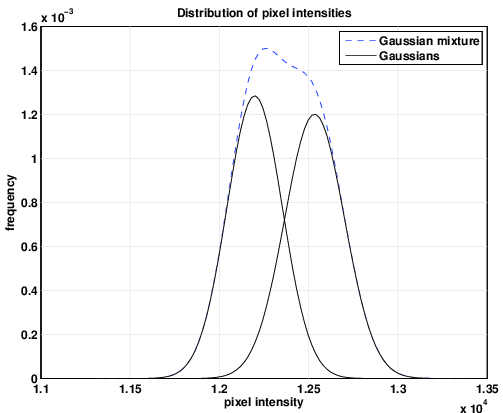
\includegraphics[width=0.5\textwidth]{figures/gaussians.png}
\caption{Density of a mixture of two normal distributions, whose means
  are the background and the fringe amplitudes, respectively.  }
\label{fig:gaussian_mixture_model}
\end{figure}

Thus the density function $f(x)$ of the intensity of an individual
pixel is modeled as follows
\begin{equation}
  f(x) = c_1\,e^{ -\frac{(x-\mu_1)^2}{2\sigma_1^2} }
  + c_2\,e^{ -\frac{(x-\mu_2)^2}{2\sigma_2^2} }.
\end{equation}

The means $\mu_1$ and $\mu_2$ ( $\mu_1 < \mu_2 = \mu_{1}+a$) are
proportional to the background amplitude and the fringe pattern
amplitude, respectively.  These values are used for normalization of
the background and fringe amplitudes before stacking.

The parameters of the two Gaussian components are estimated from the
density function of the pixel intensities by a nonlinear least squares
fit algorithm.  The algorithm requires as its input an estimated
density function.  Such an estimate is calculated in a preprocessing
step as a truncated Hermite series:
\begin{equation}
  f(x) \approx \sum_{n=0}^p \; c_n h_n\left(\frac{x - \mu}{\sigma}\right),
\end{equation}
where $h_n$ is the normalized Hermite function
\begin{equation}
  h_n(x) = {\pi}^{-\frac14} \,
  2^{-\frac{n}{2}} (n!)^{-\frac12} \, (\-1)^n \, e^{\frac{x^2\!\!}{2}} \,
  \frac{d^n}{dx^n}\left( e^{-x^2} \right),
\end{equation}
$\mu$ and $\sigma$ are, respectively, the sample mean and the sample
standard deviation of pixel intensities in the given image.  The
truncation parameter $p$ is found experimentally, $p = 20$ has been
sufficient so far.  The Hermite coefficients $c_n$ are computed as
follows
\begin{equation}
  c_n = \frac1{\sigma N}\; \sum_{i=1}^N h_n\left(\frac{I_i - \mu}{\sigma}\right),
\end{equation}
where the summation extends over all pixel intensities
$I_1, \ldots, I_{N}$, $N$ is the total number of pixels, and
$n = 0, \ldots, p$.

A detailed description of the algorithm can be found in
appendix~\ref{chap:algorithms:fringing}


\paragraph{Functions}
\label{fringe:algorithms:compute:functions}

The master fringe is computed using the following function

\begin{lstlisting}
cpl_error_code hdrl_fringe_compute(
        hdrl_imagelist          *  ilist_fringe, 
        const cpl_imagelist     *  ilist_obj,
        const cpl_mask          *  stat_mask, 
        const hdrl_parameter    *  collapse_params,
        hdrl_image              ** master, 
        cpl_image               ** contrib_map,
        cpl_table               ** qctable)
\end{lstlisting}

The output \verb+master+ and \verb+contrib_map+ products are filled
with the resulting master fringe and associated contribution map
images. The output \verb+qctable+ product contains the background
level (in table column \\ \verb+Background_level+) and the fringe
amplitude (in table column \verb+Fringe_amplitude+) computed by the
algorithm for each input image. The corresponding object data has to
be deleted by the user when not required any more.\\
Please note that if the background level and the fringe amplitude can
not be computed a warning is issued. Moreover, in this case a
background level of 0 and a fringe amplitude of 1 is assumed, i.e. the
original image is used in the following steps.

\paragraph{Inputs}
\label{fringe:algorithms:compute:inputs}

The list of images affected by fringes that should be combined to form
the master fringe is passed to the function with the hdrl imagelist
\verb+ilist_fringe+ input function-parameter.  If object masks are
needed to distinguish between sky and object pixels (very important!)
they can be passed with the cpl imagelist \verb+ilist_obj+ input
function-parameter.  Moreover, if a static mask is needed to
distinguish between regions with prominent and weak fringes it can be
passed with the cpl mask \verb+stat_mask+ input function-parameter.

Please note that the static mask \verb,stat_mask, and the object masks
\verb,ilist_obj, are optional input function-parameters, i.e. one can
pass NULL if no mask should be used.

The \verb+collapse_params+ parameter controls the collapsing algorithm
of the master fringe computation and is a \verb+hdrl_parameter+. Its
type defines the collapse method which is applied. Currently available
are the following collapsing parameter creation utilities:
\begin{itemize}\itemsep-1pt \parskip0pt \parsep0pt\small
\item \verb+hdrl_collapse_mean_parameter_create()+
\item \verb+hdrl_collapse_median_parameter_create()+
\item \verb+hdrl_collapse_weighted_mean_parameter_create()+
\item \verb+hdrl_collapse_sigclip_parameter_create(kappa_low, kappa_high, niter)+
\item \verb+hdrl_collapse_minmax_parameter_create(nlow, nhigh)+
\item \verb+hdrl_collapse_mode_parameter_create(histo_min, histo_max, bin_size,+\\\verb+mode_method, error_niter)+
\end{itemize}

Note that these parameters are dynamically allocated and must be
deleted when not needed.  For convenience HDRL provides preallocated
parameters for collapsing operations (e.g. \verb+HDRL_COLLAPSE_MEAN+)
which do not require any additional parameters. These can be used
anywhere a regular parameter can be used (deletion with
\verb+hdrl_parameter_delete+ has no effect on them). See
section~\ref{sec:imagelist:collapsing} for more details.

\paragraph{Outputs}
\label{fringe:algorithms:compute:outputs}

The result is a \verb+hdrl_image+ stored in the function-parameter
\verb+master+ containing the master fringe and its associated error as
well as an integer contribution map (\verb+contrib+) counting how many
values contributed to each pixel of the image. Moreover, the output
table \verb+qctable+ contains the derived background level in the
table column \verb+Background_level+ and the fringe amplitude in table
column \verb+Fringe_amplitude+ for each input image.


\subsubsection{Master fringe correction}
\label{fringe:algorithms:correct}

This algorithm scales and subtracts a master fringe from a sequence of
images.

\paragraph{Algorithm - short description}
\label{fringe:algorithms:correct:short}

The function subtracts a passed master fringe image
(\verb,masterfringe,) from a set of input images
(\verb,ilist_fringe,). The amplitude of the fringes is computed for
each input image and used to properly rescale the correction image
before subtraction.

The algorithm computes fringe amplitudes for each individual image by
a least squares fit of a linear combination of the estimated
master-fringe and a constant background.  Specifically, the $i$th
fringe $F_i$ is estimated as
\begin{equation}
  F_{i} = a_{i}F + b_{i},
\end{equation}
where $F$ is the estimated stacked master-fringe, and $b_i$ is a
constant representing the background.  The unknown constants $a_i$ and
$b_i$ are computed by a standard least squares fit preformed over the
unmasked pixels.

Moreover, different masks controlling the algorithm in different
stages can be passed to the hdrl function e.g. a static mask
(\verb,stat_mask,) to exclude regions where the fringe is weak -
sometimes essential for an accurate scaling estimation of noisy
images. The algorithm combines the bad pixel map (from
\verb,ilist_fringe),, the object mask (from \verb,ilist_obj,), and
static mask (\verb,stat_mask,) for the scaling computation of the
master fringe, but only uses the bad pixel map when subtracting the
master-fringe. The object mask and static mask are ignored in this
step. This ensures that the master fringe is properly subtracted (with
error propagation) in all regions not affected by the bad pixel mask.

Please note, that the function directly works on the passed hdrl
imagelist (\verb,ilist_fringe,) in order to save memory thus modifying
this imagelist i.e. removing the fringes directly from
\verb,ilist_fringe,. Moreover, the scaling factor derived and used in
this function is considered to be noiseless, i.e. the associated error
is supposed to be zero.

A detailed description of the algorithm can be found in
appendix~\ref{chap:algorithms:fringing}

\paragraph{Functions}
\label{fringe:algorithms:correct:functions}

The fringe correction is done by the following function

\begin{lstlisting}
cpl_error_code hdrl_fringe_correct(
        hdrl_imagelist          *  ilist_fringe, 
        const cpl_imagelist     *  ilist_obj,
        const cpl_mask          *  stat_mask, 
        const hdrl_image        *  masterfringe,
        cpl_table               ** qctable);
\end{lstlisting}

The function one-by-one scales and subtracts the passed master-fringe
image \verb,masterfringe, from the images stored in
\verb,ilist_fringe,. The output \verb+qctable+ product contains the
background level (in table column \verb+Background_level+) and the
fringe amplitude (in table column \verb+Fringe_amplitude+) computed by
the algorithm for each input image. The corresponding object data has
to be deleted by the user when not required any more.\\
Please note that if the background level and the fringe amplitude can
not be computed a warning is issued. Moreover, in this case a
background level of 0 and a fringe amplitude of 0 is assumed, i.e. no
correction will be applied to this image.



\paragraph{Inputs}
\label{fringe:algorithms:correct:inputs}


The list of images that should be fringe corrected by the master
fringe is passed to the function with the hdrl imagelist
\verb+ilist_fringe+ whereas the master-fringe is passed in the
\verb+masterfringe+ input function-parameter.

If object masks are needed to distinguish between sky and object
pixels (very important!)  they can be passed with the cpl imagelist
\verb+ilist_obj+ input function-parameter.  Moreover, if a static mask
is needed to distinguish between regions with prominent and weak
fringes it can be passed with the cpl mask \verb+stat_mask+ input
function-parameter.  Please note that the static mask \verb,stat_mask,
and the object masks \verb,ilist_obj, are optional input
function-parameters, i.e. one can pass NULL if no mask should be used.

\paragraph{Outputs}
\label{fringe:algorithms:correct:outputs}

The algorithm directly modifies the input hdrl images
\verb+ilist_fringe+ when performing the fringe correction, thus the
result is stored in the latter. Moreover, the output
table \verb+qctable+ contains the derived background level in the
table column \verb+Background_level+ and the fringe amplitude in table
column \verb+Fringe_amplitude+ for each input image.

\subsection{Object catalogue generation}
\label{catalogue:main}

In order to provide astrometric and photometric calibration
information, the \HDRL implements a functionality to generate a
catalogue of detected objects (i.e. stars, galaxies).

Objects are detected and parametrised using the processed input image
(\verb+img+) and confidence map (\verb+cnf+). A confidence map is
similar to a weight map. It gives an indication of the relative
quantum efficiency of each pixel, rather than an indication of the
Poisson uncertainty on the pixel flux and should be normalised to a
mean of 100. ``Bad'' pixels (either dead or hot) are given a confidence
value of zero. If stacked images are used, then the confidence map of
each single image should be propagated in order to get a confidence
map of the mosaic image. This confidence map should then be
re-normalized to a mean of 100 and passed to the routine as confidence
map.

A high-level summary of the implemented data reduction sequence is:
\begin{itemize}
\item estimate the local sky background over the image and track any
    variations at adequate resolution to eventually remove them,
\item detect objects/blends of objects and keep a list of pixels
    belonging to each blend for further analysis (see \cite{Irwin85}
    for details)
  \item parametrise the detected objects, i.e. perform astrometry,
    photometry and a shape analysis.
\end{itemize}

\subsubsection{Algorithm - short description}


If requested, (\verb+bkg_estimate+) the possibly-varying sky
background is estimated and removed automatically, prior to object
detection, using a combination of robust iteratively-clipped
estimators.

Any variation in sky level over the frame is dealt with by forming a
coarsely sampled background map grid (specified by
\verb+bkg_mesh_size+).  Within each background grid pixel, an
iteratively k-sigma clipped median value of `sky' is computed based on
the flux values within the grid pixel zone. A robust estimate of sigma
is computed by using the Median of the Absolute Deviation (MAD) from
the median. This will then be further processed to form the frame
background image.

After removing the (possibly) varying background component, a similar
robust estimate of the average sky level and sky noise per pixel is
made. This allows to robustly obtain the detection threshold for
object analysis.

Individual objects are detected using a ``standard match'' filter
approach. Since the only sources difficult to locate are those
marginally above the sky noise, to assume (after factoring in the
confidence map information) the noise as uniform, is a good
approximation. The majority of objects detected in this way 
will have a shape dominated by the point spread function (PSF), 
which thereby defines the filter to use (controlled by 
\verb+bkg_smooth_fwhm+.)

To be detected an object should consist of at least
\verb+obj_min_pixels+ contiguous pixels above a threshold controlled
by \verb+obj_threshold+ $\times$ sky-rms. Moreover, one can also
activate a deblending algorithm (\verb+obj_deblending+) in order to
disentangle overlapping objects.

Pixels are weighted in the catalogue generation according to their
value in the confidence map.  Hence if a pixel is marked as bad, then
it is not included in the flux computation over the aperture.  
The number of bad pixels
with an aperture is reported in the 'Error\_bit\_flag' column of the
output table.  The presence of bad pixels will also be reflected in
the average confidence for the aperture (column 'Av\_conf').

Please note that one also has to specify the effective gain
(\verb+det_eff_gain+) and the (\verb+det_saturation+) limit to the
routine. The gain is mainly used for the error estimation of the
various object measurements whereas the saturation limit is used to
mark and exclude saturated pixels.

%
%
%
%
%    \verb+obj_min_pixels+
%    \verb+obj_threshold+
%    \verb+obj_deblending+
%    \verb+obj_core_radius
%
%    \verb+bkg_estimate+
%    \verb+bkg_mesh_size+
%    \verb+bkg_smooth_fwhm+
%
%    \verb+det_eff_gain+
%    \verb+det_saturation+
%
%    resulttype+
%

A detailed description of the algorithm and the output table can be
found in appendix~\ref{chap:algorithms:catalogue}

 
\subsubsection{Functions}
\label{catalogue:functions}

The object catalogue, the background and the segmentation map are
computed by the following function call:

\begin{lstlisting}
hdrl_catalogue_result * hdrl_catalogue_compute(
      const cpl_image * image, 
      const cpl_image * confidence_map,
        const cpl_wcs * wcs, 
       hdrl_parameter * param)
\end{lstlisting}
             
where \verb+image+ is the input image, \verb+confidence_map+ is the
(optional) confidence map, \verb+wcs+ contains the (optional) world
coordinate system and \verb+params+ is a \verb+hdrl_parameter+
structure specifying the parameters controlling the catalogue
generation.
           
\subsubsection{Inputs}
\label{catalogue:inputs}

The input parameter to be passed to the function are created by the
following function call:

\begin{lstlisting}
hdrl_parameter * param = hdrl_catalogue_parameter_create(
      int                    obj_min_pixels,
      double                 obj_threshold, 
      cpl_boolean            obj_deblending,
      double                 obj_core_radius,
      cpl_boolean            bkg_estimate, 
      int                    bkg_mesh_size,
      double                 bkg_smooth_fwhm, 
      double                 det_eff_gain,
      double                 det_saturation,
      hdrl_catalogue_options resulttype);
\end{lstlisting}


where
  \verb+obj_min_pixels+ is the minimum pixel area for each detected object,
  \verb+obj_threshold+  is the detection threshold in sigma above sky,
  \verb+obj_deblending+ is a parameter to switch on/off deblending,\\
  \verb+obj_core_radius+ is the value of the core radius in pixels,
  \verb+bkg_estimate+  is the parameter to switch on/off the
  background estimation from the input image,
  \verb+bkg_mesh_size+ is the background smoothing box size,
  \verb+bkg_smooth_gauss_fwhm+ is the FWHM of the Gaussian kernel used
  in convolution for object detection,
  \verb+det_eff_gain+ is the detector gain value to convert ADU counts to electron counts,
  \verb+det_saturation+  is the detector saturation value, and
  \verb+resulttype+ is the \verb+hdrl_catalogue_options+ parameter which
controls the different result types. The latter is a bit-map (the
values can be combined with bitwise or) defining the computed and
returned results:

\begin{itemize}
\item \verb+HDRL_CATALOGUE_CAT_COMPLETE+: The full catalogue (see
  appendix XXX)
\item \verb+HDRL_CATALOGUE_BKG+: The background map
\item \verb+HDRL_CATALOGUE_SEGMAP+: The segmentation map
  \footnote{Contains the pixels attributed to each object, i.e. all
    pixels belonging to object XXX in the catalogue have a value of
    XXX in the segmentation map}
\item \verb+HDRL_CATALOGUE_ALL+:\\  \verb+HDRL_CATALOGUE_CAT_COMPLETE+ |
  \verb+HDRL_CATALOGUE_BKG+ | \verb+HDRL_CATALOGUE_SEGMAP+  
\end{itemize}

If a certain result type is not requested by setting the appropriate
bit-pattern, the function returns a pointer to NULL.

\subsubsection{Outputs}

The function creates an output \verb+hdrl_catalogue_result+ structure
containing the following quantities (or NULL, depending on the
hdrl\_catalogue\_options \verb+resulttype+):

\begin{lstlisting}
typedef struct {
    /* object catalogue */
    cpl_table * catalogue;
    /* segmentation map */
    cpl_image * segmentation_map;
    /* background map */
    cpl_image * background;
    /* Additional information */
    cpl_propertylist * qclist;
} hdrl_catalogue_result;
\end{lstlisting}

The \verb+hdrl_catalogue_result+ object has to be deleted by the user
when not required any more by calling the function
\verb+hdrl_catalogue_result_delete()+.

Currently the following additional informations are returned in the
cpl\_propertylist \verb+qclist+:
{\footnotesize
\begin{verbatim}
APCOR1   / Stellar aperture correction - 1/2x core flux
APCOR2   / Stellar aperture correction - core/sqrt(2) flux
APCOR3   / Stellar aperture correction - 1x core flux
APCOR4   / Stellar aperture correction - sqrt(2)x core flu
APCOR5   / Stellar aperture correction - 2x core flux
APCOR6   / Stellar aperture correction - 2*sqrt(2)x core f
APCOR7   / Stellar aperture correction - 4x core flux
APCORPK  / Stellar aperture correction - peak height
\end{verbatim}
}
and \verb+SYMBOL1+ to \verb+SYMBOL9+. 

If the symbol keywords are present in the header of the catalogue
fitsfile they are used by e.g. skycat or gaia to properly display the
objects in the image.

The APCOR keywords can be used to convert (for stellar objects) fixed
aperture fluxes to total magnitudes, as for this an aperture
correction must be applied. This correction is calculated from the
curve-of-growth and accounts for missing flux in a particular
aperture. For example, the magnitude (m) of an object using the flux
in the third bin ($i = 3$) may be calculated as

\begin{equation}
m = \tt{MAGZPT} - 2.5log_{10}(\tt{APER\_FLUX\_3/EXPTIME}) - \tt{APCOR3}
\end{equation}

With {\tt APER\_FLUX\_3} being a column in the catalogue table, {\tt
  MAGZPT} the zeropoint and EXPTIME the exposure time \footnote{For more information, refer to \url{http://casu.ast.cam.ac.uk/surveys-projects/vst/technical/catalogue-generation}}.




\subsubsection{Examples}

Detect objects on an image (img) with a given confidence map (cnf) and
wcs informations (wcs):


\begin{lstlisting}
  cpl_image * img;
  cpl_image * cnf;
  cpl_wcs * wcs;

  /* initialize the catalogue parameters */

  hdrl_parameter * p =  
       hdrl_catalogue_parameter_create(5,        /* obj_min_pixel */      
                                       2.5,      /* obj_threshold */     
                                       CPL_TRUE, /* obj_deblending */    
                                       3.0,      /* obj_core_radius */   
                                       CPL_TRUE, /* bkg_estimate */      
                                       64,       /* bkg_mesh_size */     
                                       2.0,      /* bkg_smooth_fwhm */   
                                       2.8,      /* det_eff_gain */      
                                       65200,    /* det_saturation */    
                                       HDRL_CATALOGUE_ALL);

  /* catalogue COMPUTATION */

  hdrl_catalogue_result * res = hdrl_catalogue_compute(img, cnf, wcs, p);

  /* save the catalogue, the background and the segmentation map */

  /* delete the result structure */
  hdrl_catalogue_result_delete(res);
\end{lstlisting}

\subsubsection{Catalogue Parameters in a Recipe}

In the context of a recipe, all input parameters needed by the
catalogue computation may be provided as input parameters.

The creation of \verb+cpl_parameter+ objects for the catalogue recipe interface is
facilitated by:
\begin{itemize}
\item \verb+hdrl_catalogue_parameter_create_parlist+
\item \verb+hdrl_catalogue_parameter_parse_parlist+
\end{itemize}
The former provides a \verb+cpl_parameterlist+ which can be appended
to the recipe parameter list, the latter parses the recipe parameter
list for the previously added parameters and creates a ready to use
catalogue \verb+hdrl_parameter+.

\begin{lstlisting}
 /* Create catalogue default parameters */

  hdrl_parameter * c_def =
      hdrl_catalogue_parameter_create(4, 2.5, CPL_TRUE, 5.0, CPL_TRUE, 64,
                                      2., 3.0, HDRL_SATURATION_INIT, 
                                      HDRL_CATALOGUE_ALL);
  cpl_parameterlist * s_param =
      hdrl_catalogue_parameter_create_parlist(RECIPE_NAME, "", c_def);
  hdrl_parameter_delete(c_def) ;

  for (cpl_parameter * p = cpl_parameterlist_get_first(s_param);
          p != NULL; p = cpl_parameterlist_get_next(s_param))
      cpl_parameterlist_append(self, cpl_parameter_duplicate(p));
  cpl_parameterlist_delete(s_param);
\end{lstlisting}

This will create a esorex man-page as follows:
{\footnotesize
\begin{verbatim}
esorex --man-page hdrldemo_catalogue
...
  --obj.min-pixels         : Minimum pixel area for each detected object. [4]
  --obj.threshold          : Detection threshold in sigma above sky. [2.5]
  --obj.deblending         : Use deblending?. [TRUE]
  --obj.core-radius        : Value of Rcore in pixels. [5.0]
  --bkg.estimate           : Estimate background from input, if false it is assumed
                             into is already background corrected with median 0.
                             [TRUE]
  --bkg.mesh-size          : Background smoothing box size. [64]
  --bkg.smooth-gauss-fwhm  : The FWHM of the Gaussian kernel used in convolution
                             for object detection. [2.0]
  --det.effective-gain     : Detector gain value to rescale convert intensity to
                             electrons. [3.0]
  --det.saturation         : Detector saturation value. [inf.0]
...
\end{verbatim}
}

If parlist is the recipe parameters list, we also offer a function to 
generate the Catalogue parameters directly from the recipe parameters:

\begin{lstlisting}
/* Parse the Catalogue Parameters */

hdrl_parameter * p = 
   hdrl_catalogue_parameter_parse_parlist(parlist, RECIPE_NAME);
 \end{lstlisting}

\subsection{Efficiency}
\label{efficiency:main}

This section deals with the HDRL module estimating the efficiency as a 1D function of wavelength.

The efficiency is used to monitor the system performance and health. It is calculated observing flux standard stars (in photometric conditions). Then, the observed 1D spectrum is compared with the reference spectrum, as it would be observed outside the Earth's atmosphere. The reference spectrum is provided by the user, usually via a catalog of standard stars. 


\subsubsection{Algorithm - short description}
The efficiency is calculated according to 

\begin{equation}
\epsilon(\lambda)=  \frac{I_{std}(\lambda) \cdot 10^{[ -0.4(A_p- A_m)E_x^{(r)}(\lambda)] } \cdot G \cdot E_{ph}(\lambda)}{[ T_{ex} A_{tel} I_{std-ref}^{(r)}(\lambda) ]}
\label{eq:eff}
\end{equation}
where:

\begin{itemize}

\item $I_{std}(\lambda)$ is the observed 1D spectrum [ADU] as function of wavelength [nm];

\item  $E_x^{(r)}(\lambda)$ is the resampled atmospheric extinction as function of wavelength[mag/airmass]. The wavelength is expressed in [nm]. The corresponding, user-provided spectrum will be here indicated as $E_x(\lambda)$;

\item $A_m$ is the airmass of the observed standard star spectrum;

\item $A_p$ is a parameter to indicate if the efficiency is computed at $A_m=0$ or at a given value (usually the one at which the reference standard star spectrum may be tabulated);

\item $G$ is the gain  of the detector in [e/ADU];

\item $E_{ph}(\lambda)$ is the energy of one photon at wavelength $\lambda$. $E_{ph}(\lambda)=\frac{hc}{\lambda} = \frac{1.986\cdot{}10^{-12}}{\lambda }J/{\mu}m$. $\lambda$ is expressed in ${\mu}m$;

\item $I_{std-ref}^{(r)}(\lambda)$ resampled reference standard star spectrum. The wavelength is expressed in [nm]. The corresponding, user-provided spectrum is denoted as $I_{std-ref}(\lambda)$; 

\item $h = 6.62618\cdot 10^{-34}$ Js (Planck constant);

\item $c = 2.998\cdot 10^8$ m/s (Speed of Light);

\end{itemize} 

$E_x(\lambda)$  and $I_{std-ref}(\lambda)$ are resampled by the provided routine to match the wavelengths $I_{std}(\lambda)$ is defined on. If they already match the resampling is skipped.  $\epsilon(\lambda)$ is defined for $\lambda$ only if $\lambda$ is contained in the interval $E_x(\lambda)$  and $I_{std-ref}(\lambda)$ are defined on. 

\subsubsection{Functions}
The efficiency is computed by the following function call:

\begin{lstlisting}
hdrl_spectrum1D * hdrl_efficiency_compute(const hdrl_spectrum1D * I_std,
const hdrl_spectrum1D * I_std_ref,const hdrl_spectrum1D * E_x,
const hdrl_parameter * pars)
\end{lstlisting}
where \verb+I_std+ is $I_{std}(\lambda)$, \verb+I_std_ref+ is $I_{std-ref}(\lambda)$ and \verb+E_x+ is $E_x(\lambda)$. \verb+pars+ is an \verb+hdrl_parameter+ structure containing all the other parameters required by \ref{eq:eff}, e.g. $G$.

\subsubsection{Inputs}
\label{sec:algorithms:efficiency:inputs}
The input parameter \verb+pars+ to be passed to \verb+hdrl_efficiency_compute+ is created executing the following function call:
\begin{lstlisting}
hdrl_parameter* hdrl_efficiency_parameter_create(
        const hdrl_value Ap, const hdrl_value Am, const hdrl_value G,
        const hdrl_value Tex, const hdrl_value Atel)
\end{lstlisting}
where the various input parameters are the ones in \ref{eq:eff}. Note that every parameter is an \verb+hdrl_value+, hence an error can be also provided. In that case the routine performs error propagation.

\subsubsection{Outputs}
\verb+hdrl_efficiency_compute+ creates as output a \verb+hdrl_spectrum1D+ structure, containing the calculated efficiency.

\subsubsection{Examples}
The following listing shows how the implemented HDRL function calculates the efficiency using the user-provided spectra and parameters.
The user has already provided the following spectra:

\begin{itemize}
\item \verb+I_std+: observed spectrum, wavelength in [nm];
\item \verb+I_std_ref+: model of the spectrum of the observed star, wavelength in [nm]. If defined on different wavelengths than \verb+I_std+ the function will resample it using \textit{Akima} interpolation;
\item \verb+E_x+: atmospheric extinction wavelength in [nm]. If defined on wavelengths different than \verb+I_std+ the function will resample it using \textit{Akima} interpolation \footnote{See: \url{https://www.gnu.org/software/gsl/manual/html_node/Interpolation-Types.html}}.
\end{itemize}
\begin{lstlisting}

hdrl_parameter * pars = hdrl_efficiency_parameter_create(
            (hdrl_value){1.2, 0.0},
            (hdrl_value){4.0, 0.0},
            (hdrl_value){1.0, 0.2},
            (hdrl_value){1.1, 0.0},
            (hdrl_value){2.2, 0.0});

hdrl_spectrum1D * sp_eff = hdrl_efficiency_compute(I_std, I_std_ref, 
                                                   E_x, pars);

hdrl_parameter_delete(pars); 

\end{lstlisting}

\subsubsection{Notes}
The fluxes of the observed and model spectra must be expressed in the same units. Usually the model is given in  erg/s/cm2/Angstrom. Therefore the user should correct the observed spectrum accordingly, by, e.g. a factor equal to the sampling bin size expressed in Angstrom unit.



\subsection{Response}
\label{response:main}

This section deals with the HDRL module estimating the response as a 1D function of wavelength.

\subsubsection{Algorithm - short description}
The algorithm is divided in two parts: \textit{Telluric correction} and \textit{Response calculation}. In the provided implementation the \textit{Telluric correction} is optional and can be disabled by the user.

\paragraph{Telluric Correction}

The Telluric Correction functionality tries to find the best telluric model among the ones provided and uses it to correct the observed spectrum.
The steps of the algorithm are as follows and they are repeated for each telluric model. The steps are grouped in two: \textit{Spectrum correction} and \textit{Quality evaluation}.

\textbf{Spectrum correction: }aims to correct the observed spectrum with the provided telluric model.
\begin{enumerate}
\item Convert wavelength scale (in nm) of the telluric model and the
  observation to natural logarithm if the ration $\lambda$/FWHM is
  constant. A strong prerequisite is that the sampling step of the
  logarithmic wavelength scale is very fine for both spectra to
  provide proper sampling. These resampled spectra are used only for
  the cross correlation described below;
\item Extract the range of wavelengths needed to calculate the cross correlation (water vapour feature of medium strength);
\item Cross correlate the telluric model with the observation spectrum
  over the extracted range. The cross correlation is needed to
  determine the shift and difference in resolution between the
  telluric model spectrum and the observation;
\item Fit a Gaussian around the cross correlation peak: finding the shift between the two spectra in sub-pixel precision and the FWHM;
\item Repeat the previous two steps refining the cross-correlation interval around the identified peak position;
\item Shift the telluric model by the shift obtained by the previous step;
\item Create a Gaussian kernel of size equal to the measured FWHM;
\item Convolve the shifted telluric model with the Gaussian kernel
  (this assumes that the resolution of the telluric model is much
  higher than that of the observation);
\item Convert the shifted and convolved telluric model to linear wavelength space (if needed). Resample it using integration to the wavelengths of the observed spectrum;
\item Divide the observed spectrum by the convolved and shifted telluric model: this is the \textit{corrected observed spectrum};
\end{enumerate}

\textbf{Quality evaluation: } aims to evaluate the quality of the \textit{corrected observed spectrum} calculated in the previous step.
\begin{enumerate}
\item Using the predefined continuum points, fit a spline to the \textit{corrected observed spectrum} without smoothing;
\item Divide the \textit{corrected observed spectrum} by the continuum fit;
\item Calculate the mean $m_r$ of this ratio, skipping high absorption
  areas as well as regions without telluric absorption. 
\end{enumerate}

The quantity $q = |m_r - 1|$ is used as quality indicator for the fit of the telluric model. The model having the lowest $q$ is deemed the best and its corresponding \textit{corrected observed spectrum} is used in the \textit{Response calculation} step. 
If telluric correction is disabled by the user, the \textit{Response calculation} step uses the unmodified observed spectrum.

\paragraph{Response Calculation}

\textbf{Velocity compensation: } this step can be disabled by the user and it is divided in two steps.
\begin{enumerate}
\item Determine the radial velocity of the observed (possibly telluric- corrected) spectrum by fitting a Gaussian to a known stellar line;
\item Apply the radial velocity to the stellar model spectrum as $\lambda = \lambda_0(1+\frac{RV}{c})$.
\end{enumerate}


The remaining steps to complete the response calculation are:
\begin{enumerate}
\item Calculate the raw response as described in equation \ref{eq:resp};
\item Define fit points at which the median of the flux within a given window is determined, avoiding region of very {high telluric absorption} as well as the cores of the stellar lines;
\item Fit a spline through the points determined in the previous step.
\end{enumerate}

The response is calculated according to 

\begin{equation}
R(\lambda)=  \frac{I_{std-ref}^{(r)}(\lambda) \cdot 10^{[ 0.4(A_p- A_m)E_x^{(r)}(\lambda)] } \cdot G \cdot T_{ex}}{I_{std}(\lambda)}
\label{eq:resp}
\end{equation}
where:

\begin{itemize}

\item $I_{std}(\lambda)$ is the observed 1D spectrum [ADU] as function of wavelength [nm]. If telluric correction is enabled, 

\item  $E_x^{(r)}(\lambda)$ is the resampled atmospheric extinction [mag/airmass] as function of wavelength [nm]. The corresponding, user-provided spectrum is denoted as $E_x(\lambda)$;

\item $A_m$ is the airmass of the observed standard star spectrum;

\item $A_p$ is a parameter to indicate if the response is computed at $A_m=0$ or at a given value (usually the one at which the reference standard star spectrum may be tabulated);

\item $G$ is the gain  of the detector in [ADU/e];

\item $I_{std-ref}^{(r)}(\lambda)$ resampled reference standard star spectrum. The wavelength is expressed in [nm]. The corresponding, user-provided spectrum is denoted as $I_{std-ref}(\lambda)$; 
\end{itemize} 

$E_x(\lambda)$  and $I_{std-ref}(\lambda)$ are resampled by the provided routine to match the wavelengths $I_{std}(\lambda)$ is defined on. If they already match the resampling is skipped. $R(\lambda)$ is defined for $\lambda$ only if $\lambda$ is contained in the interval $E_x(\lambda)$  and $I_{std-ref}(\lambda)$ are defined on. 

\subsubsection{Functions}
The response is computed by the following function call:

\begin{lstlisting}
hdrl_response_result *
hdrl_response_compute(
        const hdrl_spectrum1D * obs_s,
        const hdrl_spectrum1D * ref_s,
        const hdrl_spectrum1D * E_x,
        const hdrl_parameter * telluric_par,
        const hdrl_parameter * velocity_par,
        const hdrl_parameter * calc_par,
        const hdrl_parameter * fit_par)
\end{lstlisting}

\subsubsection{Inputs}
\label{sec:algorithms:response:inputs}
The input parameters to be passed to \verb+hdrl_response_compute+ are created executing the following function calls:

\begin{lstlisting}

hdrl_parameter * telluric_par = 
hdrl_response_telluric_evaluation_parameter_create(telluric_models,
        x_corr_w_step, xcorr_half_win, xcorr_normalize, 
        xcorr_is_shift_in_log, quality_areas, fit_areas, 
        lmin, lmax);
\end{lstlisting}


\verb+telluric_par+ contains the parameters needed to perform the telluric correction, the parameters can be divided in parameters needed to perform che cross-correlation, and hence determine the shift, and parameters needed to calculate the quality of the fit.



\begin{lstlisting}
hdrl_parameter * velocity_par = 
hdrl_spectrum1D_shift_fit_parameter_create(velocity_wguess,
    		velocity_range_wmin, velocity_range_wmax, 
    		velocity_fit_wmin, velocity_fit_wmax, 
    		velocity_fit_half_win);
\end{lstlisting}


\verb+velocity_par+ contains the parameters needed to perform the velocity correction.



\begin{lstlisting}
hdrl_parameter * calc_par = 
hdrl_response_parameter_create(Ap, Am, G, Tex);
\end{lstlisting}


\verb+calc_par+ contains the parameters needed to calculate the result of \ref{eq:resp}.



\begin{lstlisting}
hdrl_parameter * fit_par =
    hdrl_response_fit_parameter_create(11, fit_points, 
	fit_wrange, high_abs_regions);
\end{lstlisting}


\verb+fit_par+ contains the parameters needed to execute the final fit, after \ref{eq:resp} is performed.




\subsubsection{Outputs}
The function returns a struct of type \verb+hdrl_response_result+ containing the response as an \verb+hdrl_spectrum1D+ and other parameters that can be used for QC purposes. For a complete description of such parameters, please, refer to the documentation of \verb+hdrl_response_result+.

\subsubsection{Examples}
The following listing shows how to calculate the efficiency using the user-provided spectra and parameters.
The user has already provided the following spectra:
\begin{itemize}
\item \verb+I_std+: observed spectrum, wavelength in [nm];
\item \verb+I_std_ref+: model of the spectrum of the observed star, wavelength in [nm]. If defined on different wavelengths than \verb+I_std+ the function will resample it using \textit{Akima} interpolation;
\item \verb+E_x+: atmospheric extinction wavelength in [nm]. If defined on different wavelengths than \verb+I_std+ the function will resample it using \textit{Akima} interpolation \footnote{See: \url{https://www.gnu.org/software/gsl/manual/html_node/Interpolation-Types.html}}.
\end{itemize}
\begin{lstlisting}

hdrl_parameter * telluric_par = 
hdrl_response_telluric_evaluation_parameter_create(telluric_models,
        x_corr_w_step, xcorr_half_win, xcorr_normalize, 
        xcorr_is_shift_in_log, quality_areas, fit_areas, 
        lmin, lmax);

hdrl_parameter * velocity_par = 
hdrl_spectrum1D_shift_fit_parameter_create(velocity_wguess,
    		velocity_range_wmin, velocity_range_wmax, 
    		velocity_fit_wmin, velocity_fit_wmax, 
    		velocity_fit_half_win);
    		
hdrl_parameter * calc_par = 
hdrl_response_parameter_create(Ap, Am, G, Tex);

hdrl_parameter * fit_par =
    hdrl_response_fit_parameter_create(11, fit_points, 
	fit_wrange, high_abs_regions);

hdrl_response_result *
response_res = hdrl_response_compute(
            		I_std, 
            		I_std_ref,
            		E_x,
            		telluric_par,
            		velocity_par,
            		calc_par ,
            		fit_par);

hdrl_parameter_delete(telluric_par);
hdrl_parameter_delete(velocity_par);
hdrl_parameter_delete(calc_par);
hdrl_parameter_delete(fit_par);

/*... use the content of response_res  */

hdrl_response_result_delete(response_res);

\end{lstlisting}

\subsubsection{Notes}
\begin{itemize}
\item The fluxes of the observed and model spectra must be expressed in the same units. Usually the model is given in  erg/s/cm2/Angstrom. Therefore the user should correct the observed spectrum accordingly, by, e.g. a factor equal to the sampling bin size expressed in Angstrom unit;
\item The response should be determined in optimal (photo-metric) atmospheric conditions.
Furthermore, in case of different modes, the results of one mode cannot be compared with the results of the other. For example, if the observation facility has support for a Laser Guide Star (LGS) observation can be obtained either using LGS or using a Natural Guide Star (NGS). Results obtained with NGS cannot be compared with the ones obtained with LGS;
\item Observations should be obtained in the same optical setting mode.
\end{itemize}

\subsection{Differential Atmospheric Refraction (DAR)}
\label{refraction:main}

The effects of atmospheric refraction can be readily seen in any spectrograph or IFU. Atmospheric refraction will displace a source, or its spectrum, 
by an amount that is dependent on the source wavelength and the angular distance of the source from the zenith.  
This effect is due to the stratified density structure of our atmosphere, and the displacement will be toward the zenith and will be largest for shorter wavelengths.
Because of this latter attribute, differential atmospheric refraction is not generally associated with infrared instruments. However, it can be 
readily seen in SINFONI data cubes observed with the largest wavelength coverage (H+K) and in the smallest pixel scales (25 mas). 
Here, the shift can be as large as 6 pixels from the beginning of the data cube to its end (see Figures \ref{fig:SINFONI_trace} and \ref{fig:SINFONI_image}).

This module uses an analytical approach to compute the expected differential refraction as a function of wavelength, zenith angle, and the refractive index of air
which, in turn, depends on temperature, pressure, and water vapour pressure.

The {\tt hdrl\_dar} routines require the following inputs (all of which are, generally, available in the input data headers):
\begin{itemize}
\item the ambient atmospheric parameters: temperature, pressure, and humidity as contained in the environmental keyword headers:
TEL.AMBI.TEMP, TEL.AMBI.PRES.START/END, and TEL.AMBI.RHUM, respectively.
\item the instrument rotation angle on the sky
\item the parallactic angle of instrument
\item and, the world-coordinate system (WCS)
\end{itemize}

With this input, the differential atmospheric refraction is calculated (optionally, also with an error propagation), and provides an output of the $X$ and $Y$-axis shifts as a function of the
\verb+cpl_vector+ with the input wavelengths.  The resulting shift corrections can be directly apply to the pixel image in order to correct this effect.
The next section describes the algorithms used to make this calculation.


\subsubsection{Algorithm - short description}

This module contains routines to calculate the refractive index of air \footnote{See: \url{https://emtoolbox.nist.gov/Wavelength/Documentation.asp\#AppendixA}, for the formulae used.}. 
The main loop compute the differential refractive offset for the input reference wavelengths, and stores the shift in the coordinates, taking into account the instrument rotation angle 
on the sky and the parallactic angle at the time of observation.

The differential atmospheric refraction is calculated according to the algorithm from Filippenko (1982, PASP, 94, 715). This algorithm uses the Owens formula 
which converts relative humidity in water vapour pressure. 


\paragraph{Owens saturation pressure}

This function computes the saturation pressure using the J.C. Owens calibration (1967, Applied Optics, 6, 51-59). 
The saturation pressure is given by:

\begin{equation}
s_p = -10474 +116.43\ T -0.43284\ T^2 +0.00053840\ T^3
\label{eq:owens}
\end{equation}

where verb+T+ is the temperature in Kelvins.


\paragraph{Filippenko refractive index}

At sea level (P=760 \verb+mm Hg+ , T = 15 $^oC$) the refractive index of dry air is given by (Edl\'en 1953; Coleman, Bozman, and Meggers 1960):
\begin{equation}
(n( \lambda )_{15,760}-1)10^6 = 64.328 + \frac{29498.1}{146-(1/ \lambda )^2} +\frac{255.4}{41-(1/ \lambda )^2}
\end{equation}
where $\lambda$ is the wavelength of light in vacuum (microns). Since observatories are usually located at high altitudes, the index of refraction must be corrected for the 
lower ambient temperature and pressure (P) (Barrell 1951):
\begin{equation}
(n(\lambda)_{T,P} -1) = (n(\lambda)_{15,760} - 1) \cdot \frac{P[1+(1.049-0.0157\ T) 10^{-6}\ P]}{720.883 (1+0.003661\ T)}
\end{equation}

In addition, the presence of water vapour in the atmosphere reduces $(n-1)10^6$ by:
\begin{equation}
\frac{0.0624-0.000680/\lambda^2}{1 + 0.003661\ T} f
\end{equation}
where $f$ is the water vapour pressure in mm of Hg, and T is the air temperature in $^oC$ (Barrell 1951) and is expressed as:

\begin{equation}
f = 0.75006158 \cdot s_p \cdot h
\end{equation}
where $s_p$ is the saturation pressure of equation \ref{eq:owens} and $h$ is the relative humidity in \verb+[%]+.


\subsubsection{Function}

The differential atmospheric refraction is computed by the following function:
\begin{lstlisting}
cpl_error_code hdrl_dar_compute(
        const hdrl_parameter * params,
        const hdrl_value       lambdaRef, 
        const cpl_vector     * lambdaIn,
        cpl_vector           * xShift, 
        cpl_vector           * yShift, 
        cpl_vector           * xShiftErr, 
        cpl_vector           * yShiftErr)
\end{lstlisting}

The output products contain the resulting differential atmospheric refraction, and include the shift in pixels (with their associated error).
This results can be directly apply to the original image.
Each output value is associated at each wavelength value included in the \verb+lambdaIn+ [\AA] \verb+cpl_vector+.
The Filipenko method uses the value \verb+lambdaRef+ [\AA] as the reference wavelength from which the differential atmospheric
refraction is computed.  In other words, the \verb+xShift and yShift+ values will be zero at \verb+lambdaRef+.   Generally, \verb+lambdaRef+
is chosen to be the mid-point of the wavelength range covered by the input data.


\subsubsection{Inputs}
\label{sec:algorithms:refraction:inputs}
The input parameters to be passed to \verb+hdrl_dar_compute+ are created by executing the following function

\begin{lstlisting}
hdrl_parameter * hdrl_dar_parameter_create(
        hdrl_value             airmass,
        hdrl_value             parang,
        hdrl_value             posang,
        hdrl_value             temp,
        hdrl_value             rhum,
        hdrl_value             pres, 
        cpl_wcs              * wcs)
\end{lstlisting}


The input parameters of the function are:
\begin{itemize}
  \item \verb+airmass+: Air mass.
  \item \verb+parang+: Parallactic angle during exposure [deg].
  \item \verb+posang+: Position angle on the sky [deg].
  \item \verb+temp+: Temperature [$^o$C].
  \item \verb+rhum+: Relative humidity [\%].
  \item \verb+pres+: Pressure [mbar].
  \item \verb+wcs+: World coordinate system [deg].
\end{itemize}
Note that every parameter is an \verb+hdrl_value+, hence an error can be also provided and the routine supports error propagation.
See section \ref{sec:algorithms:refraction:parameters} for a summary of the error input parameters in terms of the esorex call to this recipe.

\textit{Please note that during the testing of the algorithm it was
  discovered that the propagated errors in the source shifts, computed
  when the error of the temperature (temp.error) and pressure
  (pres.error) are specified, are over-estimated.  We are currently
  investigating the source of this over-estimate and expect to be able
  to repair it soon.  The core functionality of the algorithm, in
  computing the expected source shifts due to atmospheric refraction,
  are not affected by this issue.}

\subsubsection{Outputs}
\label{sec:algorithms:refraction:outputs}

The function fills several input/output \verb+cpl_vector+ structures that contain the shift and error in each data axis.

This values are associated with each wavelength in the \verb+lambdaIn+ \verb+cpl_vector+ and they can be applied directly to the image.
The user is free to apply these values either as a continuous corrective shift to the data (requiring, of course, interpolation), or to round the
shifts to integer values and shift the data to a pixel grid.


\subsubsection{Example}
\label{sec:algorithms:refraction:example}
This section briefly describes the actual call to the function.

\begin{lstlisting}
/* Declare and init variables */
hdrl_value airmass, parang, posang, temp, rhum, pres;
cpl_wcs *wcs = cpl_wcs_new_from_propertylist(plPri);
...
/* Create hdrl_parameter from call the main function */
hdrl_parameter *h_par = hdrl_dar_parameter_create(
      airmass, parang, posang, temp, rhum, pres, wcs);
...
/* Declare and init the input (lambdaIn) and outputs cpl_vector */
cpl_vector *lambdaIn, *xShift, *yShift, *xShiftErr, *yShiftErr;
...
/* Execute main funtion and clean memory*/
hdrl_dar_compute(h_par, lambdaRef, lambdaIn,
      xShift, yShift, xShiftErr, yShiftErr);
hdrl_parameter_delete(h_par);
\end{lstlisting}


\subsubsection{DAR Parameters in a Recipe}
\label{sec:algorithms:refraction:parameters}

In the context of a recipe, all input parameters needed by the differential atmospheric refraction computation may be provided as input parameters. 
This will create a esorex man-page as follows:
{\footnotesize
  \begin{verbatim}
  $ esorex --man-page hdrldemo_dar
  
  --maxRatioNaNsInImage : Max ratio [%] between bad pixels (NaNs) and good pixels. [30.0]
  --lambdaRef-err       : Error [%] of the reference lambda. [0.0]
  --parang-err          : Error [%] of the parallactic angle. [0.0]
  --posang-err          : Error [%] of the position angle. [0.0]
  --temp-err            : Error [%] of the temperature. [0.0]
  --rhum-err            : Error [%] of the relative humidity. [0.0]
  --pres-err            : Error [%] of the pressure. [0.0]
  --airm.method         : Method of approximation to calculate airmass. 
                                <HARDIE_62 | YOUNG_IRVINE_67 | YOUNG_94> [HARDIE_62]
  --airm.ra-err         : Error [%] of the right ascension (using for calculate airmass). [0.0]
  --airm.dec-err        : Error [%] of the declination (using for calculate airmass). [0.0]
  --airm.lst-err        : Error [%] of the local sideral time (using for calculate airmass). [0.0]
  --airm.exptime-err    : Error [%] of the integration time (using for calculate airmass). [0.0]
  --airm.geolat-err     : Error [%] of the latitude (using for calculate airmass). [0.0]
  \end{verbatim}
}
where the parameters listed include:
\begin{itemize}
    \item  \verb+--maxRatioNaNsInImage+ allows the selection of valid images.  An image having a ratio of NaNs greater than that specified by \verb+--maxRatioNaNsInImage+ will be excluded
    from the analysis.
    \item \verb+--lambdaRef-err+ to \verb+--pres-err+ to set errors to the input parameters for DAR, that allow for the computation of error propagation.
    \item \verb+--airm.method+ for the selection of the method to used to approximate the airmass (see section \ref{airmass:main} for a more detailed description).
    \item \verb+--airm.ra-err+ to \verb+--airm.geolat-err+ to set the errors in the airmass calculation, that allow for the computation of error propagation (see section \ref{airmass:main} for a more detailed description).
\end{itemize}

\subsection{Effective air mass}
\label{airmass:main}

This section explains how the \verb+hdrl_utils+ module can be used to calculate the effective air mass of an observation. It can be calculated using one of three different methods: 
Hardie (1962), Young \& Irvine (1967) and Young (1994).


\subsubsection{Algorithm - short description}

The algorithm calculates the average airmass for the line-of-sight given by the right ascension (aRA) and the declination (aDEC). The latitude (aLatitude) of the observatory site 
and the local sidereal time (aLST) at the beginning of the observation has to be given, as well as the duration of the observation, i.e. the exposure time (aExptime). 
If the exposure time is zero then only one value of airmass is computed, instead of weighting the beginning, middle, and end of the exposure according to Stetson (Stetson P., 1987, PASP 99, 191).

This function can calculate three different kinds of approximations to the airmass as specified in the\\ 
\verb+hdrl_airmass_approx+ parameter\footnote{You can find these and other collections of interpolative approximations formulas in \url{http://en.wikipedia.org/w/index.php?title=Airmass\&oldid=358226579\#Interpolative_formulas}.}:
\begin{enumerate}
  \item The formula given by Hardie (Hardie 1962, In: "Astronomical Techniques", ed. Hiltner, p. 184) to compute the airmass as a function of zenith distance.
  \item The formula of Young and Irvine (Young A. T., Irvine W. M., 1967, Astron. J. 72, 945), where the range of trustworthy airmass outputs is limited to between 1 and 4.
  \item The formula of Young (Young A. T., 1994 ApOpt, 33, 1108).
 \end{enumerate}  

This algorithm can take into account the error propagation if the user enters the relative error of the input parameters in a \verb+hdrl_value+ structure \{data,error\}.


\paragraph{Zenith distance}

Computes the zenith distance for an observation. It needs the hour angle, declination, and latitude (all in $[rad]$).

\begin{lstlisting}
hdrl_value hdrl_get_zenith_distance(
          hdrl_value aHourAngle, 
          hdrl_value aDelta, 
          hdrl_value aLatitude)
\end{lstlisting}

The function computes the cosine of the zenith distance for an observation taken at an hour angle (\verb+aHourAngle+) from the meridian, with valid values in the range extending from $-\pi$ to $\pi$, and the declination (\verb+aDelta+) with possible values between $-0.5\ \pi$ and $0.5\ \pi$. The latitude (\verb+aLatitude+) of the observing site takes values in the range of $0$ to $2\ \pi$.


\paragraph{Hardie approximation (1962)}

Compute the airmass with the \verb+Hardie+ approximation. It need the secant of the zenith distance.

\begin{lstlisting}
hdrl_value hdrl_get_airmass_hardie(hdrl_value hvaSecZ)
\end{lstlisting}

The function uses the approximation given by Hardie (Hardie 1962, In: "Astronomical Techniques", ed. Hiltner, p. 184) to compute the airmass as a function of zenith angle which is given in terms of its secant (\verb+hvaSecZ+). It is supposedy more accurate than Young \& Irvine (1967), and usable for zenith angles below 80 degrees.
  

\paragraph{Young \& Irvine approximation (1967)}
Compute the airmass with the \verb+Young & Irvine+ approximation. It need the secant of the zenith distance.

\begin{lstlisting}
hdrl_value hdrl_get_airmass_youngirvine(hdrl_value hvaSecZ)
\end{lstlisting}

This function uses the approximation given by Young \& Irvine (Young A. T., Irvine W. M., 1967, Astron. J. 72, 945) to compute the airmass for a given sec(z) (\verb+hvaSecZ+). 
This approximation takes into account atmospheric refraction and curvature but is, in principle, only valid at sea level.
  
  
\paragraph{Young approximation (1994)}

Computes the airmass using the \verb+Young+ approximation. It needs the cosine of the true zenith distance.

\begin{lstlisting}
hdrl_value hdrl_get_airmass_young(hdrl_value hvaCosZt)
\end{lstlisting}

This function uses the approximation given by Young (Young A. T., 1994 ApOpt, 33, 1108) to compute the relative optical airmass as a function of true, rather than refracted, 
zenith angle which is given in terms of its cosine (\verb+hvaCosZt+). It is supposedly more accurate than \verb+Young & Irvine+ (1967) but restrictions aren't known.


\subsubsection{Functions}
\label{sec:algorithms:airmass:inputs}

The differential atmospheric refraction is computed by the following function:

\begin{lstlisting}
hdrl_value hdrl_utils_airmass(
        hdrl_value          aRA, 
        hdrl_value          aDEC, 
        hdrl_value          aLST,
        hdrl_value          aExptime, 
        hdrl_value          aLatitude,
        hdrl_airmass_approx type)
\end{lstlisting}
where \verb+type+ is the method of airmass approximation to use.

The input parameters of the function are:
\begin{itemize}
  \item \verb+aRA+: right ascension [deg].
  \item \verb+aDEC+: declination [deg].
  \item \verb+aLST+: local sideral time elapsed since siderial midnight [s].
  \item \verb+aExptime+: integration time [s].
  \item \verb+aLatitude+: latitude of the observatory site [deg].
  \item \verb+type+: method of airmass approximation.
\end{itemize}

The valid values for \verb+type+ are:
\begin{lstlisting}
typedef enum {
        HDRL_AIRMASS_APPROX_HARDIE       = 1,	
        HDRL_AIRMASS_APPROX_YOUNG_IRVINE = 2,
        HDRL_AIRMASS_APPROX_YOUNG        = 3
} hdrl_airmass_approx;
\end{lstlisting}

Note that every parameter is an \verb+hdrl_value+, hence an error can be also provided and the routine supports error propagation.


\subsubsection{Outputs}
\label{sec:algorithms:airmass:outputs}
The algorithm returns the computed average airmass, or the \verb+hdrl_parameter+ value \{-1,\ 0.\} when an error is encountered.


\subsubsection{Example}
\label{sec:algorithms:airmass:example}

An example of an airmass calculation is given here:

\begin{lstlisting}
/* Aproximation methods */
hdrl_airmass_approx type = HDRL_AIRMASS_APPROX_HARDIE;

/* Example of input parameters */
hdrl_value ra       = {122.994945,   0.};
hdrl_value dec      = {74.95304,     0.};
hdrl_value lst      = {25407.072748, 0.};
hdrl_value exptime  = {120.,         0.};
hdrl_value geolat   = {37.2236,      0.};

/* Set variation of error in variables */
double delta        = 1.;
double deltaRa      = delta/100.;
double deltaDec     = delta/100.;
double deltaLst     = delta/100.;
double deltaExptime = delta/100.;
double deltaGeolat  = delta/100.;

/* Set error propagation variables */
ra.error            = deltaRa      * fabs(ra.data);
dec.error           = deltaDec     * fabs(dec.data);
lst.error           = deltaLst     * fabs(lst.data);
exptime.error       = deltaExptime * fabs(exptime.data);
geolat.error        = deltaGeolat  * fabs(geolat.data);

/* Calcule airmass */
hdrl_value airm = hdrl_utils_airmass(ra, dec, lst, exptime, geolat, type);
\end{lstlisting}

\subsection{Fixed Pattern Noise (fpn)}
\label{patternnoise:main}

This section describes how HDRL identifies regular
noise on detector data. A classical example is provided by the pick noise,
i.e. low-amplitude, quasi-periodical patterns super-imposed on the
normal read-noise. It is due to electronic interference and might show
up or disappear on short timescales (days or hours).

Those artifacts are visible only on the detector data but of course
exist also on other calibration data and on science data where they
may compromise the detector sensitivity.


\subsubsection{Algorithm - short description}

The algorithm implements three steps that can be described as follows:

\begin{enumerate}\itemsep-1pt \parskip0pt \parsep0pt\small
\item Derive the power spectrum of the image using the Fast Fourier
  Transform (FFT):
    \begin{eqnarray*}
      fft                 & = & FFT\_2D(\ img\ ) \\
      power\_spec         & = & abs(\ fft\ )^2
    \end{eqnarray*}
  \item Mask the peak of the power spectrum that corresponds to 
    the pixel-to-pixel variations. By default only one pixel
    placed in the corner on the bottom left is masked (the DC
    component), but more pixels can be masked providing an
    optional bad pixel mask, e.g. if there is a pixel-to-pixel 
    cross talk on longer spatial scale).
    \begin{eqnarray*}
      power\_spec\_filter & = & filter\_peak(\ power\_spec,\ 1,\ 1\ )
    \end{eqnarray*}
  \item Calculate the standard deviation $std$ and the standard
    deviation based on the Median Absolute Deviation (MAD) $std_{mad}$
    of the power spectrum by taking the masked regions into account:
    \begin{eqnarray*}
      std                  & = & stdev(\ power\_spec\_filter\ ) \\
      std_{mad}             & = & mad(\ power\_spec\_filter\ ) * 1.4826
    \end{eqnarray*}
\end{enumerate}

As mentioned above, when computing the standard deviation and the
MAD-based standard deviation on the power spectrum the algorithm
excludes the masked region. For this the user can provide an optional
mask \verb+mask_in+ or use the \verb+dc_mask_x+ and \verb+dc_mask_y+
function parameter to create one on the fly. The mask created on the
fly will start at pixel (1,1) and extend in both direction up to
(\verb+dc_mask_x+, \verb+dc_mask_y+)\footnote{Please note that in the
  current implementation the power spectrum contains the DC component
  (the DC term is the 0 Hz term and is equivalent to the average of
  all the samples in the window) in pixel (1,1).}. Moreover, the mask
created on the fly by setting \verb+dc_mask_x+ and \verb+dc_mask_y+
and the optional mask (\verb+mask_in+) are combined and are both taken
into account when calculating the statistics (\verb+std+ and
\verb+std_mad+). Furthermore, the final (combined) mask is attached to
the returned \verb+power_spectrum+ image as normal cpl\_mask and can
be retrieved with the CPL function \verb+cpl_image_get_bpm(power_spectrum)+

\newpage

\subsubsection{Function}

The power spectrum and it's statistics are computed by the following
function:
\begin{lstlisting}
cpl_error_code hdrl_fpn_compute(
        cpl_image       *  img_in,
        const cpl_mask  *  mask_in,
        const cpl_size     dc_mask_x,
        const cpl_size     dc_mask_y,
        cpl_image       ** power_spectrum,
        double          *  std,
        double          *  std_mad)
\end{lstlisting}

The \verb+power_spectrum+ pointer is filled by the function with an
allocated image which must be deleted by the user when not required
anymore.

%
%Possible #_cpl_error_code_ set in this function:
%- CPL_ERROR_NULL_INPUT          If img_in is NULL
%- CPL_ERROR_ILLEGAL_INPUT       If dc_mask_x < 1 or dc_mask_y < 1
%- CPL_ERROR_ILLEGAL_INPUT       If the power_spectrum is NOT NULL
%- CPL_ERROR_ILLEGAL_INPUT       If img_in contains bad pixels
%- CPL_ERROR_INCOMPATIBLE_INPUT  If mask NOT NULL and size(mask) != size(img_in)


\subsubsection{Inputs}
\label{sec:algorithms:fpn:inputs}

The following function parameters have to be passed to the
hdrl\_fpn\_compute function:
\begin{itemize}\itemsep-1pt \parskip0pt \parsep0pt\small
\item \verb+img_in+: the input image. Please note that bad pixels are
  not allowed
\item \verb+mask_in+ (or \verb+NULL+): an optional mask which is used
  when deriving the standard deviations on the power spectrum
\item \verb+dc_mask_x+: x-pixel window (>= 1) to discard DC component
  starting form pixel (1, 1)
\item \verb+dc_mask_y+: y-pixel window (>= 1) to discard DC component
  starting from pixel (1, 1)
\end{itemize}

\subsubsection{Outputs}
\label{sec:algorithms:fpn:outputs}

The result is the computed power spectrum (\verb+power_spectrum+),
the standard deviation (\verb+std+) of the power spectrum, the MAD
based standard deviation of the power spectrum (\verb+std_mad+) and
the final mask used to compute \verb+std+ and \verb+std_mad+ which can
be retrieved with \verb+cpl_image_get_bpm(power_spectrum)+

Please note that the \verb+power_spectrum+ pointer is filled by the
function with an allocated image which must be deleted by the user
when not required anymore.

\subsubsection{Example}
\label{sec:algorithms:fpn:example}
This section briefly describes the call to the function. For a more
detailed implementation please see also the \verb+hdrldemo_fpn+
example recipe.

{\footnotesize
\begin{lstlisting}
/* Load the image and the (optional) mask */
cpl_mask  *mask_in = cpl_mask_load(...);
cpl_image *img_in  = cpl_image_load(...);


/* Compute the power spectrum and the statistics */
cpl_image *power_spectrum  = NULL;
double    std       = -1.;
double    std_mad   = -1.;

hdrl_fpn_compute(img_in, mask_in, dc_mask_x, dc_mask_y,
                 &power_spectrum, &std, &std_mad);

/* save the power spectrum and the used mask */
...

/* Cleanup the memory  */
cpl_image_delete(power_spectrum);
cpl_image_delete(img_in);
cpl_mask_delete(mask_in);
\end{lstlisting}
}

\newpage

\subsection{Image and Cube Resampling}
\label{resampling:main}

A common problem in astronomy is the resampling of 2D images and 3D cubes onto a
common grid. Ideally, this is done only once in the data reduction workflow as
each sub-pixel resampling redistributes the flux and creates correlation. In the
resampling \HDRL project we would like to address two different
scenarios. Assuming that one would like to re-grid and stack 10 dithered images/cubes
with pre-determined World Coordinate System (WCS). Then one should be able to:

\begin{itemize}
\item Combine all images/cubes in a single cloud of points (we use a
table for this step - see below) and when creating the resampled output
image/cube all information is used in a single interpolation step, i.e. no
image-by-image interpolation is done.
\item Resample each individual image/cube on the same output grid (image by image
interpolation) and combine the single resampled images in a second step with
hdrl stacking methods.
\end{itemize}
Both scenarios interpolate only once, but the second scenario is important in
case not all bad pixels could be properly determined and inserted in the bad
pixel mask upfront. Then the implemented HDRL pixel resampling function offers the possibility to use a robust pixel
combination method (median or $\kappa\sigma$~clipping) to combine the
images/cubes. 

\subsubsection{Algorithm - short description}
\label{resampling:algorithms}

The implemented interpolation algorithms are based on the MUSE pipeline and work
for 2D images and 3D cubes. The 2D and 3D interpolation is done in 2-dimensional
and 3-dimensional spaces, respectively. Currently there are six different
interpolation methods implemented:

\begin{center}
\begin{itemize}
\item {\bf Nearest:} Nearest  resampling
\item {\bf Linear:} Weighted resampling using an inverse distance weighting function
\item {\bf Quadratic:} Weighted resampling using a quadratic inverse distance weighting function
\item {\bf Renka:} Weighted resampling using a Renka weighting function
\item {\bf Drizzle:} Weighted resampling using a drizzle-like weighting scheme
\item {\bf Lanczos:} Weighted resampling using a lanczos-like restricted sinc as weighting function
\end{itemize}
\end{center}

\paragraph{Nearest Neighbour}
\label{resampling:algorithms:nearest}
The algorithm does not use any weighting function but simply uses the value of
the nearest neighbour inside an output voxel\footnote{In 3D computer graphics, a voxel represents a value on a regular grid in three-dimensional space. See \http{https://en.wikipedia.org/wiki/Voxel} for more information.} centre as the final output value. If
there is no nearest neighbour inside the voxel (but e.g. only outside), the voxel
is marked as bad. This speeds up the algorithm considerably. There are no
control parameter for this method.

\paragraph{Linear}
\label{resampling:algorithms:linear}
The algorithm uses a linear inverse distance weighting function ($\frac{1}{r}$)
for the interpolation. The parameter \verb+loop_distance+ controls the number of
surrounding pixels that are taken into account on the final grid, e.g. a
\verb+loop_distance+ of 1 uses 3 pixels (x - 1, x, x + 1) in each dimension,
i.e.  9 in total for a 2D image and 27 in total for a 3D cube. Moreover, if the
parameter \verb+use_errorweights+ is set to TRUE, an additional weight, defined
as 1/variance, is taken into account\footnotemark.
 
\paragraph{Quadratic}
\label{resampling:algorithms:quadratic}
The algorithm uses a quadratic inverse distance weighting function
($\frac{1}{r^2}$) for the interpolation. The parameter \verb+loop_distance+
controls the number of surrounding pixels that are taken into account on the
final grid, e.g. a \verb+loop_distance+ of 1 uses 3 pixels (x - 1, x, x + 1) in
each dimension, i.e.  9 in total for a 2D image and 27 in total for a 3D
cube. Moreover, if the parameter \verb+use_errorweights+ is set to
TRUE, an additional weight, defined as 1/variance,
is taken into account\footnotemark[\value{footnote}].
 
\paragraph{Renka}
\label{resampling:algorithms:renka}
The algorithm uses a modified Shepard-like distance weighting function following
Renka for the interpolation. The parameter \verb+critical_radius+ defines the
distance beyond which the weights are set to 0 and the pixels are therefore not
taken into account. The parameter \verb+loop_distance+ controls the number of
surrounding pixels that are taken into account on the final grid, e.g. a
\verb+loop_distance+ of 1 uses 3 pixels (x - 1, x, x + 1) in each dimension,
i.e.  9 in total for a 2D image and 27 in total for a 3D cube. Moreover, if the
parameter \verb+use_errorweights+ is set to TRUE,
an additional weight, defined as 1/variance, is taken into account\footnotemark[\value{footnote}].

\paragraph{Drizzle}
\label{resampling:algorithms:drizzle}
The algorithm uses a drizzle-like distance weighting function for the
interpolation. The down-scaling factors \verb+pix_frac_x+, \verb+pix_frac_y+,
and \verb+pix_frac_lambda+, for x, y, and wavelength direction control the
percentage of flux of the original pixel/voxel that drizzles into the target
pixel/voxel. The parameter \verb+loop_distance+ controls the number of
surrounding pixels that are taken into account on the final grid, e.g. a
\verb+loop_distance+ of 1 uses 3 pixels (x - 1, x, x + 1) in each dimension,
i.e.  9 in total for a 2D image and 27 in total for a 3D cube. Moreover, if the
parameter \verb+use_errorweights+ is set to TRUE,
an additional weight defined as 1/variance is taken into account\footnotemark[\value{footnote}].

\paragraph{Lanczos}
\label{resampling:algorithms:lanczos}
The algorithm uses a restricted $sinc$ distance weighting function
($\frac{sinc(r)}{sinc(r/kernel\_size)}$) with the kernel size given by the
parameter \verb+kernel_size+ for the interpolation. The parameter
\verb+loop_distance+ controls the number of surrounding pixels that are taken
into account on the final grid, e.g. a \verb+loop_distance+ of 1 uses 3 pixels
(x - 1, x, x + 1) in each dimension, i.e.  9 in total for a 2D image and 27 in
total for a 3D cube. Moreover, if the parameter \verb+use_errorweights+ is set
to TRUE, an additional weight defined as
1/variance is taken into account\footnotemark[\value{footnote}].



\footnotetext{Please note that only if the variance of a pixel is $> 0$ this
  additional weight is applied}

\subsubsection{Functions}
The input data is resampled using the following function call
\begin{lstlisting}
hdrl_resample_result * hdrl_resample_compute(
        const cpl_table     * restable,
        hdrl_parameter      * method,
        hdrl_parameter      * outputgrid,
        const cpl_wcs       * wcs);
\end{lstlisting}

The routine is not directly working on an image or a cube but on a table
(\verb+restable+). For 2D images, the table is created by the function
\verb+hdrl_resample_image_to_table()+, whereas for a 3D data cube the
function \verb+hdrl_resample_imagelist_to_table()+ generates the appropriate
table. In the case that many images/cubes have to be combined into a single
mosaic, the two functions can be called multiple times and the returned tables
should be merged into a single table by using \verb+cpl_table_insert()+.

\subsubsection{Inputs}
The \verb+hdrl_resample_compute+ function has four arguments:

\paragraph*{restable}
The first function argument \verb+restable+ is a \verb+cpl_table+ with
information on the data to be resampled.  It can be created in case of a 2D
image or a 3D data cube with the following function call:

\begin{lstlisting}
cpl_table * hdrl_resample_image_to_table(
        const hdrl_image     * hima,
        const cpl_wcs        * wcs);  
\end{lstlisting}

\begin{lstlisting}
cpl_table * hdrl_resample_imagelist_to_table(
        const hdrl_imagelist * himlist,
        const cpl_wcs        * wcs);
\end{lstlisting}

where \verb+ hima+ is a hdrl image containing the 2D image and \verb+ himlist+ a
hdrl imagelist containing the 3D cube that should be resampled. The \verb+wcs+
is a cpl wcs object that encodes the world coordinate system of the given
image/cube. 


In case the above mentioned functions can not be used to create the table
(e.g. the pixel to sky mapping is very complex and can not be encoded by the cpl
wcs object) the pipeline developer has to create and fill the table. The table should be
created and initialised as follows:

{
\footnotesize
\begin{lstlisting}
  tab = cpl_table_new(size);
  
  /* create the table columns */
  cpl_table_new_column(tab, HDRL_RESAMPLE_TABLE_RA,     HDRL_RESAMPLE_TABLE_RA_TYPE);
  cpl_table_new_column(tab, HDRL_RESAMPLE_TABLE_DEC,    HDRL_RESAMPLE_TABLE_DEC_TYPE);
  cpl_table_new_column(tab, HDRL_RESAMPLE_TABLE_LAMBDA, HDRL_RESAMPLE_TABLE_LAMBDA_TYPE);
  cpl_table_new_column(tab, HDRL_RESAMPLE_TABLE_DATA,   HDRL_RESAMPLE_TABLE_DATA_TYPE);
  cpl_table_new_column(tab, HDRL_RESAMPLE_TABLE_BPM,    HDRL_RESAMPLE_TABLE_BPM_TYPE);
  cpl_table_new_column(tab, HDRL_RESAMPLE_TABLE_ERRORS, HDRL_RESAMPLE_TABLE_ERRORS_TYPE);

  /* init column values */
  cpl_table_fill_column_window_double(tab, HDRL_RESAMPLE_TABLE_RA,    0, size, 0.);
  cpl_table_fill_column_window_double(tab, HDRL_RESAMPLE_TABLE_DEC,   0, size, 0.);
  cpl_table_fill_column_window_double(tab, HDRL_RESAMPLE_TABLE_LAMBDA,0, size, 0.);
  cpl_table_fill_column_window_double(tab, HDRL_RESAMPLE_TABLE_DATA,  0, size, 0.);
  cpl_table_fill_column_window_int(tab,    HDRL_RESAMPLE_TABLE_BPM,   0, size, 0);
  cpl_table_fill_column_window_double(tab, HDRL_RESAMPLE_TABLE_ERRORS,0, size, 0.);
\end{lstlisting}
}

Please note that the interpolation function \verb+hdrl_resample_compute()+ was
only tested with tables created by \verb+hdrl_resample_image_to_table()+ or
\verb+hdrl_resample_imagelist_to_table()+, i.e. mappings encoded by a cpl wcs
object. Creating and using a handcrafted table could lead to side effects that the
interpolation function cannot properly handle.


\paragraph*{method}
Currently six different interpolation methods can be used to resample the data. The corresponding hdrl parameter \verb+method+ is created executing the
appropriate function call:

\begin{itemize}

\item {\bf Nearest:} Nearest neighbour resampling (see
section~\ref{resampling:algorithms:nearest}) 
\begin{lstlisting}
hdrl_parameter * hdrl_resample_parameter_create_nearest(void);
\end{lstlisting}

\item {\bf Linear:} Weighted resampling using inverse distance weighting
function (see section~\ref{resampling:algorithms:linear})
\begin{lstlisting}
hdrl_parameter * hdrl_resample_parameter_create_linear(
        const int    loop_distance,
        cpl_boolean  use_errorweights);  
\end{lstlisting}

\verb+loop_distance+: in pixel units ($>= 0$) \\ 
\verb+use_errorweights+: cpl\_boolean (CPL\_TRUE or CPL\_FALSE)  

\item {\bf Quadratic:} Weighted resampling using quadratic inverse distance
        weighting function (see section~\ref{resampling:algorithms:quadratic})
\begin{lstlisting}
hdrl_parameter * hdrl_resample_parameter_create_quadratic(
        const int    loop_distance,
        cpl_boolean  use_errorweights);  
\end{lstlisting}

\verb+loop_distance+: in pixel units ($>= 0$) \\ 
\verb+use_errorweights+: cpl\_boolean (CPL\_TRUE or CPL\_FALSE)  

\item {\bf Renka:} Weighted resampling using Renka weighting function (see
        section~\ref{resampling:algorithms:renka}) 
\begin{lstlisting}
hdrl_parameter * hdrl_resample_parameter_create_renka(
        const int    loop_distance,
        cpl_boolean  use_errorweights,
        const double critical_radius);  
\end{lstlisting}

\verb+loop_distance+: in pixel units ($>= 0$) \\ 
\verb+use_errorweights+: cpl\_boolean (CPL\_TRUE or CPL\_FALSE)\\  
\verb+critical_radius+: in pixel units ($> 0$) 

\item {\bf Drizzle:} Weighted resampling using a drizzle-like weighting scheme
        (see section~\ref{resampling:algorithms:drizzle}) 
\begin{lstlisting}
hdrl_parameter * hdrl_resample_parameter_create_drizzle(
        const int    loop_distance,
        cpl_boolean  use_errorweights,
        const double pix_frac_x,
        const double pix_frac_y,
        const double pix_frac_lambda);
  
\end{lstlisting}
      
\verb+loop_distance+: in pixel units ($>= 0$) \\ 
\verb+use_errorweights+: cpl\_boolean (CPL\_TRUE or CPL\_FALSE)\\  
\verb+pix_frac_x+: fraction of pixel/voxel ($> 0$) \\ 
\verb+pix_frac_y+: fraction of pixel/voxel ($> 0$) \\ 
\verb+pix_frac_lambda+: fraction of pixel/voxel ($> 0$) \\ 

\item {\bf Lanczos:} Weighted resampling using a lanczos-like restricted sinc
        for weighting (see section~\ref{resampling:algorithms:lanczos}) 
\begin{lstlisting}
hdrl_parameter * hdrl_resample_parameter_create_lanczos(
        const int   loop_distance,
        cpl_boolean use_errorweights,
        const int   kernel_size);
\end{lstlisting}

\verb+loop_distance+: in pixel units ($>= 0$) \\ 
\verb+use_errorweights+: cpl\_boolean (CPL\_TRUE or CPL\_FALSE)\\  
\verb+kernel_size+: in pixel units ($> 0$) 
\end{itemize}


\paragraph*{outputgrid}
The \verb+outputgrid+ parameter defines basic properties of the resampled
image/cube. Depending on the input data (image or cube) the \verb+outputgrid+
parameter should be created with the appropriate function call,
i.e. \\ \verb+hdrl_resample_parameter_create_outgrid2D_userdef()+ for an image
and \\ \verb+hdrl_resample_parameter_create_outgrid3D_userdef()+ for a
cube. For convenience, the \verb+outputgrid+ parameter can also be created with
\verb+hdrl_resample_parameter_create_outgrid2D()+ or
\verb+hdrl_resample_parameter_create_outgrid3D()+. In this case, only the step
sizes in right ascension (\verb+delta_ra+), declination (\verb+delta_dec+) and
wavelength (\verb+delta_lambda+) of the output image/cube have to be given. All
the rest is automatically derived from the data by the
\verb+hdrl_resample_compute()+ function. The four functions read as follows:

\begin{lstlisting}
hdrl_parameter * hdrl_resample_parameter_create_outgrid2D_userdef(
        const double delta_ra,
        const double delta_dec,
        const double ra_min,
        const double ra_max,
        const double dec_min,
        const double dec_max,
        const double fieldmargin);  
\end{lstlisting}

\begin{lstlisting}
hdrl_parameter * hdrl_resample_parameter_create_outgrid3D_userdef(
        const double delta_ra,
        const double delta_dec,
        const double delta_lambda,
        const double ra_min,
        const double ra_max,
        const double dec_min,
        const double dec_max,
        const double lambda_min,
        const double lambda_max,
        const double fieldmargin);
\end{lstlisting}

where \verb+delta_ra+, \verb+delta_dec+, and \verb+delta_lambda+ are the output
grid steps in right ascension, declination and wavelength. Moreover, these two
functions allow the user to set the full output grid by defining
\verb+ra_min+, \verb+ra_max+,  \verb+dec_min+, \verb+dec_max+, and
\verb+lambda_min+, \verb+lambda_max+. These parameters define the minimum and
maximum boundaries of the output image in terms of right ascension, declination
and wavelength. Furthermore, with the parameter \verb+fieldmargin+ one can add a
margin to the output image in all spacial directions.

The parameters \verb+delta_ra+, \verb+delta_dec+, \verb+ra_min+, \verb+ra_max+,
\verb+dec_min+, and \verb+dec_max+ have to be given in degrees [deg], whereas the
parameters \verb+delta_lambda+, \verb+lambda_min+, and \verb+lambda_max+ have to
be given in meter [m]. The \verb+fieldmargin+ has to be given in percent with 0
adding no margin to the output image/cube

For convenience, the \HDRL also offers the following convenience functions that
calculate the boundaries of the output image/cube from the data and
automatically set the fieldmargin:


\begin{lstlisting}
hdrl_parameter * hdrl_resample_parameter_create_outgrid2D(
        const double delta_ra,
        const double delta_dec);  
\end{lstlisting}

\begin{lstlisting}
hdrl_parameter * hdrl_resample_parameter_create_outgrid3D(
        const double delta_ra,
        const double delta_dec,
        const double delta_lambda);  
\end{lstlisting}

\paragraph*{wcs}
This input parameter specifies the World Coordinate System which should be
representative of the images that are going to be resampled. The resampling
functions uses the wcs input (CD matrix) mostly do determine the scales between
the input and output grid. Please note, that in case the user would like to
combine images/cubes with substantially different pixel sizes into a single
output image/cube, the single tables have to be properly scaled to the same
scales before merging them into the final table.


\subsubsection{Outputs}
\label{sec:algorithms:resampling:outputs}

The \verb+hdrl_resample_compute()+ function creates an output
\verb+hdrl_resample_result+ structure containing the following quantities:

\begin{lstlisting}
typedef struct {
        /* cpl propertylist containing the output wcs information */
        cpl_propertylist * header;
        /* hdrl imagelist containing the data, the errors, and the bpm */
        hdrl_imagelist   * himlist;
} hdrl_resample_result;
\end{lstlisting}

This structure contains for convenience a cpl propertylist \verb+header+ with
the output wcs that can directly be used by the cpl saving functions to save the
image/cube. In case the wcs object itself is needed, the cpl function
\verb+cpl_wcs_new_from_propertylist(header)+ should be used. Moreover, the
structure contains the resampled image/cube as hdrl imagelist \verb+himlist+. If
a 2D image was resampled, the returned imagelist is of size 1 and the resampled
hdrl image can be accessed with \verb+hdrl_imagelist_get(himlist, 0)+.

The \verb+hdrl_resample_result+ object has to be deleted by the user
when not required any more by calling the function
\verb+hdrl_resample_result_delete()+.

Please note that the output is using the Gnomonic projection\footnote{see
  \url{https://en.wikipedia.org/wiki/Gnomonic_projection}}. The gnomonic
projection is from the centre of a sphere to a plane tangential to the
sphere. The sphere and the plane touch at the tangent point. This in encoded in
the header file by:
\begin{lstlisting}
  CTYPE1  = 'RA---TAN'           / Gnomonic projection
  CTYPE2  = 'DEC--TAN'           / Gnomonic projection
\end{lstlisting}

\newpage
\subsubsection{Example}
\label{sec:algorithms:resampling:example}
This section briefly describes a typical cube regridding example .
{\footnotesize
  \begin{lstlisting}
  /* Load input data, errors and bpm frames */
  cpl_imagelist* imlist_data  = cpl_imagelist_load(name, CPL_TYPE_DOUBLE, extension_data);
  cpl_imagelist* imlist_error = cpl_imagelist_load(name, CPL_TYPE_DOUBLE, extension_error);
  cpl_imagelist* imlist_bpm   = cpl_imagelist_load(name, CPL_TYPE_INT, extension_bpm);
  
  /* Load input wcs */
  cpl_propertylist *xheader_data = cpl_propertylist_load(name, extension_data);
  cpl_wcs *wcs = cpl_wcs_new_from_propertylist(xheader_data);
  cpl_propertylist_delete(xheader_data);
  
  /* Add the bad pixel mask to the corresponding cpl image */
  cpl_size size = cpl_imagelist_get_size(imlist_data);
  for(cpl_size k = 0; k < size; k++) {
     cpl_image* data = cpl_imagelist_get(imlist_data, k);
     cpl_image* bpm  = cpl_imagelist_get(imlist_bpm, k);
     cpl_mask*  mask = cpl_mask_threshold_image_create(bpm, 0, INT_MAX);
     cpl_image_reject_from_mask(data, mask);
     cpl_mask_delete(mask);
     cpl_imagelist_set(imlist_data, data, k);
  }

   /* Create the hdrl imagelist and free memory */
  hdrl_imagelist* hlist = NULL;
  hlist = hdrl_imagelist_create(imlist_data, imlist_error);
  hdrl_imagelist_delete(imlist_data);
  hdrl_imagelist_delete(imlist_error);
  hdrl_imagelist_delete(imlist_bpm);
  
  /* store the imagelist information into the cpl_table and free memory */
  cpl_table* restable  = hdrl_resample_imagelist_to_table(hlist, wcs);
  hdrl_imagelist_delete(hlist);
  
  /* Define the output grid */
  hdrl_parameter *outgrid = NULL;
  outgrid = hdrl_resample_parameter_create_outgrid2D(5.5e-05, 5.5e-05, 2.8e-10);

  /* define the method - here LANCZOS */
  hdrl_parameter *method = NULL;
  method = hdrl_resample_parameter_create_lanczos(1, CPL_FALSE, 2);
  
  /* Do the resampling */
  hdrl_resample_result *result = NULL;
  result = hdrl_resample_compute(restable, method, outgrid, wcs);

   /* save the relevant results */
...
   /* Cleanup the memory */
   hdrl_parameter_delete(method);
   hdrl_parameter_delete(outgrid);
   hdrl_resample_result_delete(result);
   cpl_wcs_delete(wcs);
   cpl_table_delete(restable);
\end{lstlisting}
}

\subsubsection{Additional Information}

As mentioned above, the \verb+hdrl_resample_compute+ function requires as an
input a cpl table and not hdrl images or an hdrl imagelist. This choice was made
for flexibility but comes with a cost on the memory consumption.  Moreover, the
current implementation does not distinguish between a 2D image and a 3D cube in
the table structure, i.e. the wavelength column is always filled. Furthermore,
cpl functions are usually used to read the input images and they are then
inserted into a hdrl image, which implies a small overhead.

We can understand the requirements in term of memory consumption as follows.
In the typical use case the developer has input three cubes: one containing the data, stored in a float\footnote{usually 4 bytes} data type, one the error, stored in a float data type, and the bad pixels, stored in an integer\footnote{usually 4 bytes} data type.
Then the \verb+cpl_imagelist+ objects are inserted into a hdrl imagelist
which has the data and error in double precision and each has a bpm in
unsigned~char\footnote{usually 1 bytes} precision [see step 2. below].
Then the information of the hdrl imagelist is stored into a cpl table [see
step 3. below].
Finally one has to define and fill the hdrl imagelist containing the
final resampled image/cube [see step 4. below].
The size of the resampled image
[step 4. below] strongly depends on the use-case: i.e. if the input images/cubes
are mostly stacked, or if a mosaic is created and, if a mosaic is created,
its size strongly depends on possible gaps between the CCDs.


\begin{enumerate}
\item cpl\_imagelist (read the raw data x, y, $\lambda$)
\begin{itemize}
\item data (float) + error (float) + bpm (int) \textbf{[requires $\approx 3 \times float$]}
\end{itemize}
\item $\Rightarrow$ hdrl\_imagelist (join the raw data/error/bpm)
\begin{itemize}
\item $\Rightarrow$ data ($2\times$ float) + error ($2\times$ float) + bpm
($2\times$ unsigned char $\approx 0.5 \times float$) \textbf{[requires $\approx 4.5 \times float$]}
\end{itemize}
\item $\Rightarrow$ cpl\_table (transform raw data x, y, $\lambda$ $\rightarrow$
Ra, Dec, $\lambda$)
\begin{itemize}
\item Ra ($2\times$ float) + Dec ($2\times$ float) + $\lambda$ ($2\times$ float) + data ($2\times$ float) + error ($2\times$ float) + bpm (int)  \textbf{[requires $\approx 11 \times float$]}
\end{itemize}
\item $\Rightarrow$ hdrl\_imagelist (resample Ra, Dec, $\lambda$  $\rightarrow$ x, y, $\lambda$)
\begin{itemize}
\item $\Rightarrow$ data ($2\times$ float) + error ($2\times$ float) + bpm
($2\times$ unsigned char $\approx 0.5 \times float$) \textbf{[requires $\approx 4.5 \times float$]}
\end{itemize}
\end{enumerate}

After reading the data [step 1.] and inserting the data into an hdrl imagelist
[step 2.] the data of step 1. can be deleted. The total image consumption of the
transition of step 2 and step 3 depends on the data. If you have multi extension
frames like for VIRCAM you can populate the table extension by extension and
therefore you are mostly dominated by the size of your table. If you can not
work extension by extension, e.g. if your input is a MUSE cube you can delete
the hdrl imagelist of step 2 only after you fully populate the cpl table of
step 3. This means that you have to keep the data involved in step 2 and
step 3 in memory at the same time\footnote{see section
\ref{sec:largedata:buffer} for a possibility to
address this problem}. Then, once the table is filled, you may delete the hdrl
imagelist created in step 2. As written above, the size of the resampled image [step 4.]
strongly depends on the use-case so here we assume that the resampled image is a
mosaic without gaps in between (no stacking). Then for transition between
steps 3 and 4 one needs to have the table and the resampled output image in
memory at the same time.

Usually, memory (RAM) requirements are dominated by the data allocated in step 2~+~3  or step 3~+~4. This means that as a rule of thumb one would
need \textbf{[$\approx 11 + 4.5 = 15.5 \times float \times \mbox{number of input pixels}$]} of memory.

This shows that if your data requires a certain amount of RAM to be stored as
raw data you need \textbf{at
least 6 times more memory}: $3\times$ float $\Rightarrow$ $15.5 \times$
float, to perform the corresponding resampling. Please note, that in case you
do not have error images/cubes and/or bpm
images/cubes in input you have to assume that they also would be there, when you
calculate the maximum amount of memory consumption as previously described.
Even if you pass NULL to the hdrl\_imagelist\_create() function, it will
then create an error and bpm image on the fly. In other words, if you only have
information on the input data (no error and no bpm), you need
\textbf{at least 18 times more memory} to do the resampling.




\subsection{Limiting Magnitude}
\label{sec:algorithms:maglim:main}

The limiting magnitude is one of the mandatory header keywords in the
Phase 3 archival
standard\footnote{see \url{https://www.eso.org/sci/observing/phase3.html}
for the ESO Phase 3 Standard} and characterizes the depth of an
observation. According to the ESO Phase 3 standard, it is defined as
the magnitude of a unresolved source whose flux is 5 times the noise
background, i.e. the magnitude of a point like source detected with
$\frac{S}{N}=5$.

\subsubsection{Algorithm - short description}
\label{sec:algorithms:maglim:algo}

The limiting magnitude of an image is determined as follows:

\begin{itemize}
\item The input image \verb+image+ is convolved with a Gaussian kernel
  specified by the input parameters \verb+fwhm+ (the FWHM of the
  kernel), \verb+kernel_size_x+, and \verb+kernel_size_y+ (the
  extension of the kernel in x-direction and y-direction in pixel).
  To minimize border effects/artifacts during convolution, the input
  image gets enlarged by a border depending on the kernel size. The
  parameter \verb+image_extend_method+ can be used to specify the
  algorithm to compute the values of the out-of-bounds pixels during
  convolution (\verb+HDRL_IMAGE_EXTEND_NEAREST+ $\rightarrow$ use the
  nearest border pixel, \verb+HDRL_IMAGE_EXTEND_MIRROR+ $\rightarrow$
  mirror the image with respect to the border). Masked pixels are
  ignored in the convolution, i.e. the kernel is normalized ignoring
  masked pixels.
\item Compute the \verb+mode+ as described in
  section~\ref{sec:algorithms:robust_mean:mode} of the convolved
  image.
\item   Consider all the non-masked pixels in the convolved image below the MODE
(let's define them as valid pixels), and compute the noise as:
$$NOISE = 1.4826\cdot\mbox{MAD(valid pixels)}\cdot c$$

  The factor $c = \frac{1}{\sqrt{1-\frac{2}{\pi}}}\approx 1.6588967 $
  accounts for the fact that HDRL computes the statistics on half of the distribution
  (assuming a Gaussian noise distribution), MAD is the median absolute deviation,  and
  1.4826  is  the  scaling  factor to convert the MAD in the standard deviation (for a Gaussian
  distribution).  If MAD=0, then:
  
$$NOISE = \mbox{STDDEV(valid pixels)}\cdot c$$
where STDEV indicates the standard deviation.

\item Compute the limiting magnitude as:
$$ABMAGLIM = -2.5 log_{10}(5\cdot NOISE\cdot 4\pi\sigma^{2})+ZPT$$
with $\sigma = \frac{FWHM}{\sqrt{4 ln(4)}}\approx \frac{FWHM}{2.35482}$
\end{itemize}

\subsubsection{\label{sec:algorithms:maglim:functions}Functions}

The \HDRL implements the following function to derive the limiting magnitude:

\begin{lstlisting}
cpl_error_code hdrl_maglim_compute(
        cpl_image                * image,
	double                     zeropoint,
	double                     fwhm,
	cpl_size                   kernel_size_x,
        cpl_size                   kernel_size_y,
	hdrl_image_extend_method   image_extend_method,
	hdrl_parameter           * mode_parameter,
	double                   * limiting_magnitude);
\end{lstlisting}


\subsubsection{\label{sec:algorithms:maglim:inputs}Inputs}

The image where the limiting magnitude should be derived and its
zeropoint is passed to the function by the \verb+image+ and the
\verb+zeropoint+ argument.

The \verb+fwhm+ parameter sets the full width at half maximum of the
Gaussian convolution kernel whereas the extension of the kernel in
x-direction and y-direction (in pixel) is set by \verb+kernel_size_x+,
and \verb+kernel_size_y+, respectively.  The parameter
\verb+image_extend_method+ specifies the algorithm to compute the
values of the out-of-bounds pixels during convolution
(\verb+HDRL_IMAGE_EXTEND_NEAREST+ $\rightarrow$ use the nearest border
pixel, \verb+HDRL_IMAGE_EXTEND_MIRROR+ $\rightarrow$ mirror the image
with respect to the border).

The hdrl parameter \verb+mode_parameter+ controls the computation of
the mode of the distribution and is created by the
\verb+hdrl_collapse_mode_parameter_create()+ function. The parameter
of this function (\verb+histo_min+, \verb+histo_max+, \verb+bin_size+,
\verb+mode_method+, and \verb+error_niter+) are described in
section~\ref{sec:algorithms:robust_mean:mode}

Finally, the computed limiting magnitude is returned as
\verb+limiting_magnitude+
  
\subsubsection{\label{sec:algorithms:maglim:outputs}Outputs}

The result of the function is the limiting magnitude of the image
stored in the function parameter\\ \verb+limiting_magnitude+


\subsubsection{Example}
The following code is a example how to use HDRL to compute the limiting
magnitude from an image.

\begin{lstlisting}
 
 /* initialize the parameters of a the mode computation */

 double histo_min = 10.;
 double histo_max = 1.; /* min > max -> autoset by algorithm */
 double bin_size = 0.;  /* bin_size <= 0 -> autoset by algorithm */
 cpl_size error_niter = 0; /* analytic error */
 hdrl_mode_type mode_method = HDRL_MODE_MEDIAN; /* very robust */

 hdrl_parameter * mode_parameter = NULL;
 mode_parameter = hdrl_collapse_mode_parameter_create(histo_min,
                                                      histo_max,
                                                      bin_size,
                                                      mode_method,
                                                      error_niter);
                                                      
 /* initialize other parameters of the limiting magnitude computation */

 double zeropoint = 24.3;                         
 double fwhm = 3.50;
 cpl_size kernel_size_x = 10; /* about 3 times fwhm */
 cpl_size kernel_size_y = 10; /* about 3 times fwhm */
 hdrl_image_extend_method convolution_boundary = HDRL_IMAGE_EXTEND_MIRROR;
 double limiting_magnitude = 0.;
 
 /* compute the limiting magnitude */
 
 hdrl_maglim_compute(image, zeropoint, fwhm, kernel_size_x,
       			  kernel_size_y, convolution_boundary,
       			  mode_parameter, &limiting_magnitude);
                                 
\end{lstlisting}


-----------------------------------------------------------------------------
\subsection{Barycentric correction}
\label{sec:algorithms:barycorr:main}

The algorithm derives the barycentric correction of an observation,
i.e. the wavelength shift to apply to a spectrum to compensate for the
motion of the observer with respect to the barycenter of the solar
system, by using the \href{https://github.com/liberfa/erfa}{ERFA}
(Essential Routines for Fundamental Astronomy) library. ERFA is a C
library containing key algorithms for astronomy, and is based on the
\href{http://www.iausofa.org}{SOFA library} published by the
International Astronomical Union (IAU). \\

\subsubsection{Algorithm - short description}
\label{sec:algorithms:barycorr:algo}

The implemented algorithm uses the ERFA function
\href{https://github.com/liberfa/erfa/blob/master/src/apco13.c}{eraApco13()}
to calculate the barycentric correction of an observation. For details
on the implemented low level algorithm please visit the above
mentioned web pages and links therein.

A comparison between the algorithm implemented in the \HDRL and the
one implemented in the ESPRESSO pipeline shows a very good agreement.
For this about 7000 IDPs from 2021 were re-analyzed with the \HDRL
implementation and the differences read as follows:
\begin{itemize}
    \item Mean difference : 0.036 m/s
    \item Median difference: 0.055 m/s
    \item Standard deviation: 0.281 m/s
    \item MAD (median absolute deviation): 0.217 m/s
    \item Maximum deviation: 1.573 m/s
\end{itemize}

\subsubsection{Functions}
\label{sec:algorithms:barycorr:functions}

The \HDRL implements the following function to derive the barycentric correction:
\begin{lstlisting}
cpl_error_code hdrl_barycorr_compute(
        double            ra,
        double            dec,
        const cpl_table * eop_table,
        double            mjdobs,
        double            time_to_mid_exposure,
        double            longitude,
        double            latitude,
        double            elevation,
        double            pressure,
        double            temperature,
        double            humidity,
        double            wavelength ,
        double          * barycorr);
\end{lstlisting}

\subsubsection{Inputs}
\label{sec:algorithms:barycorr:inputs}

The different \textbf{input} function parameters are described as follows:
\begin{itemize}\itemsep-1pt \parskip2pt \parsep2pt
\item \verb+ra+:                     Target right ascension (J2000) in [deg]
\item \verb+dec+:                    Target declination (J2000) in [deg]
\item \verb+eop_table+:              cpl\_table containing the earth orientation parameter
\item \verb+mjdobs+:                 Start of observation in [days]
\item \verb+time_to_mid_exposure+:   Time to mid exposure, e.g. EXPTIME/2. in [s]
\item \verb+longitude+:              Telescope geodetic longitude (+ = East ) in [deg]
\item \verb+latitude+:               Telescope geodetic latitude  (+ = North) in [deg]
\item \verb+elevation+:              Telescope elevation above sea level in [m]
\item \verb+pressure+:               Pressure at the observer in [hPa == mbar]
\item \verb+temperature+:            Ambient temperature at the observer in [deg C]
\item \verb+humidity+:               Relative humidity at the observer [range 0 - 1]
\item \verb+wavelength+:             Observing wavelength in [micrometer]
\end{itemize}


Please note that the pressure, temperature, humidity, and the
wavelength parameters are only tested with a value of 0. No tests with
other values were performed.

The \verb+eop_table+ contains the
\href{https://www.iers.org/IERS/EN/Science/EarthRotation/EOP.html}{Earth
  Orientation Parameter} as a function of time (\verb+MJD-OBS+) and
can be downloaded from
\href{https://www.iers.org/IERS/EN/Home/home\_node.html}{IERS}. For
this purpose the \HDRL offers the 2 functions
\\ \verb+hdrl_download_url_to_buffer()+ and
\verb+hdrl_eop_data_totable()+. The first function allows you to
download the full EOP table from IERS and the second function extracts
and converts the relevant information into a fits table. The latter
contains the appropriate columns and can be passed to the\\
\verb+hdrl_barycorr_compute()+ function.

\begin{lstlisting}
char * hdrl_download_url_to_buffer(
       const char * url,
       size_t     * data_length);  
\end{lstlisting}
This function allows you to download a url into a c data buffer with
\verb+url+ being the url to download from. The length of the buffer
is stored in the function parameter \verb+data_length+. The url to
download the EOP data should
be \verb+https://datacenter.iers.org/products/eop/rapid/standard/finals2000A.data+

Please note, that this function is not threadsafe, to the extent that
it may only be called from the main thread, with no other threads
running. So as long as esorex or alike is not using threads it still
may be called from within a recipe before the the recipe itself, or
hdrl launches any additional threads.

\begin{lstlisting}
cpl_table * hdrl_eop_data_totable (
            const char * eop_data,
            cpl_size     data_length);
\end{lstlisting}
From the above listed
url\footnote{\url{https://datacenter.iers.org/products/eop/rapid/standard/finals2000A.data}},
this function extracts the relevant information from the c data buffer
and converts it into a fitsfile.  In this function, the
\verb+eop_data+ is the downloaded data buffer and \verb+data_length+
the length of the buffer.

As the time resolution of the EOP table is only one day, the
parameters are linearly interpolated to have the most accurate values
at the time of observation.

\subsubsection{Outputs}
\label{sec:algorithms:barycorr:outputs}

The \textbf{computed barycentric correction} is stored in the function
parameter \verb+barycorr+ with the units \verb+[m/s]+.

\subsubsection{Example}
The following code is a skeleton example on how to use HDRL to compute
the barycentric correction of an observation. For a detailed
implementation please see the esotk\_barycorr recipe for the
barycentric correction computation and the esotk\_eop recipe for
the EOP table creation.

\begin{lstlisting}
/* Load EOP file - it was created by another dedicated recipe */
/* For detail on how to create the EOP file see the esotk_eop recipe */

cpl_table * eop_table =
            cpl_table_load(cpl_frame_get_filename(eop_frame), 1, 0);

/* Read the primary header */
 cpl_propertylist * header =
            cpl_propertylist_load(cpl_frame_get_filename(cur_frame), 0);
 
 double ra        = cpl_propertylist_get_double(header, "RA");
 double dec       = cpl_propertylist_get_double(header, "DEC");
 double mjdobs    = cpl_propertylist_get_double(header, "MJD-OBS");
 double exptime   = cpl_propertylist_get_double(header, "EXPTIME");
 double longitude = cpl_propertylist_get_double(header, "ESO TEL GEOLON");
 double latitude  = cpl_propertylist_get_double(header, "ESO TEL GEOLAT");
 double elevation = cpl_propertylist_get_double(header, "ESO TEL GEOELEV");
 double pressure    = 0.0
 double temperature = 0.0
 double humidity    = 0.0
 double wavelength  = 0.0

 double barycorr = 0;
 hdrl_barycorr_compute(ra, dec, eop_table, mjdobs, exptime/2.,
                       longitude,  latitude, elevation,
                       pressure, temperature, humidity, wavelength,
                       &barycorr);
                                 
 cpl_msg_info (cpl_func, "Barycentric correction: %g m/s", barycorr);
\end{lstlisting}


%TODO


\section{Cookbook}

The cookbook contains additional help for the pipeline developer in
order to use the \HDRL in a efficient way. It might also include
recipe-level functionality as currently implemented and used in the
hdrldemo pipeline.

\begingroup
\let\cleardoublepage\relax
\let\clearpage\relax

\subsection{Handling large datasets}
\label{sec:largedata:buffer}

In order to help handling datasets larger than the available memory and swap space
HDRL provides an experimental object \verb+hdrl_buffer+ which can be used to
allocate disk backed memory maps.

It provides following functions:
\begin{itemize}
\item \verb+hdrl_buffer_new()+: create a new buffer object
\item \verb+hdrl_buffer_allocate(size_t n)+: allocate \verb+n+ bytes of memory
\item \verb+hdrl_buffer_free(void *p)+: free memory pointed to by \verb+p+,
    depending on the position in the memory pool it might actually not free the
    memory.
\item \verb+hdrl_buffer_delete(hdrl_buffer *)+: delete the buffer object and all memory it
    allocated.
\end{itemize}

It is designed to be used like a memory pool (sometimes also called memory arena
or object stack) which allows fast allocation and deletion of many objects but
the ability to delete random objects in random order is limited.
It is not threadsafe so if it is used in a multithreaded environment each
thread must create and manage its own \verb+hdrl_buffer+.

For good performance usage of this memory should be blocked to chunks of the
available RAM to avoid unnecessary disk IO.

Note that on 32 bit machines one is still limited to 4GiB of allocations due to
the address space limitations, on 64 bit machines one is only limited by the
available disk space.

Memory maps can be slower than swap space backed memory (due to higher
complexity and the kernel flushing dirty pages to disk periodically).
In order to help test the impact the buffer object will use \verb+cpl_malloc+
for memory allocation if the environment variable \verb+HDRL_BUFFER_MALLOC+ is
set.
On systems with sufficient amounts of swap space this can be the more efficient
mode of operation.

\subsubsection{Examples}
\begin{lstlisting}
hdrl_buffer * buf = hdrl_buffer_new();
/* allocate 2 GiB of memory */
void * mem = hdrl_buffer_allocate(1ull << 31ull);
void * mem2 = hdrl_buffer_allocate(100);
do_stuff(mem, mem2);
/* free all memory again */
hdrl_buffer_delete(buf);
\end{lstlisting}

HDRL provides a function \verb+hdrl_image_new_from_buffer+ to allocate a
\verb+hdrl_image+ from a \verb+hdrl_buffer+ which can be treated like a normal
image, including deletion with \verb+hdrl_image_delete+ and creation of views.

\begin{lstlisting}
hdrl_buffer * buf = hdrl_buffer_new();
hdrl_imagelist * hl = hdrl_imagelist_new()
for (size_t i = 0; i < 1000; i++) {
    hdrl_image * img = hdrl_image_new_from_buffer(2000, 2000, buf);
    hdrl_image_add_scalar(img, 5., 3.);
    hdrl_imagelist_set(hl, img, i);
}
hdrl_image * out; cpl_image * contrib;
hdrl_imagelist_collapse(hl, HDRL_COLLAPSE_MEDIAN, &out, &contrib);

/* This is very inefficient as it will need to load the data from disk
   twice, instead one should loop over the images or use the iterator
   interface to work in RAM sized blocks */
hdrl_imagelist_add_scalar(hl, 5., 3.);
hdrl_imagelist_mul_scalar(hl, 5., 3.);

/* free all memory again, note the imagelist has to be explicitly deleted
   because structure has not been allocated from the buffer */
hdrl_imagelist_delete(hl);
hdrl_buffer_delete(buf);
\end{lstlisting}



%
%\subsection{Overscan Corretion: hdrldemo\_overscan}
%
%\subsection{Master Bias computation:  hdrldemo\_bias}
%
%\subsection{Master Dark computation: hdrldemo\_bias}
%
%\subsection{Master Flatfield computation: hdrldemo\_flat}


\endgroup
%\subsection{Parameters}






\appendix
%\section{Installation}
\label{installation}


\section{Abbreviations and acronyms}
\label{ABBREVIATIONS}



\begin{tabular}{ll}
CPL    & Common Pipeline Library\\
HDRL   & High-level Data Reduction Library\\
ESOREX & ESO Recipe Execution Tool\\
PPS    & Pipeline Systems Group\\
QC     & Quality Control \\
SGDP   & Science Grade Data Product\\
SPD    & Science Products Department\\
USD    & User Support Department\\
VLT    & Very Large Telescope \\
\end{tabular}


\section{Statistical Estimators}
\label{chap:algorithms:stat_estimators}

\subsection{Arithmetic mean - Arithmetic weighted mean}
\label{sec:algorithms:robust_mean:mean}

The arithmetic mean of a sample ${x_{1}, x_{2},\dots,x_{N}}$ is
defined as
\begin{equation}
  \label{eq:mean}
  \overline{x}= \frac{1}{N}\sum_{i=1}^{N} x_{i}\,.
\end{equation}
For a random variable $X$ that is normally distributed ($N(\mu,
\sigma)$), the sample mean is the most efficient estimator of the
population mean $\mu$. By the central limit theorem this statement
holds asymptotically for many noise distributions encountered in
practice.

If the noise distribution of $X$ is unknown, its variance can be
estimated from the sample as
\begin{equation}
  \label{eq:mean:sample_variance}
  \hat{\sigma}^{2} = \frac{1}{N-1}\sum_{i=1}^{N}{(x_{i} - \overline{x})^{2}}\,.
\end{equation}
If $X$ has variance $\sigma$ then the average \eqref{eq:mean} has
variance 
\begin{equation}
  \label{eq:mean_variance}
  \sigma_{\mathrm{av}}^{2} = \frac{\sigma^{2}}{N}.
\end{equation}
This relation can be used in place of
Eq.~\eqref{eq:mean:sample_variance} if an \textit{a priori} estimate
of the noise in the images is available and is the same for all images
(homescedastic case).

When each image has its own noise image $\sigma_{i}^{2}(x,y)$
(heteroscedastic case), then the weighted mean
\begin{equation}
  \label{eq:mean_weighted}
  \overline{x} = \left(\sum
    \frac{x_{i}}{\sigma_{i}^{2}} \right)\,\left(\sum
    \frac{1}{\sigma_{i}^{2}}\right)^{-1}
\end{equation}
can be used, giving higher weight to values with lower noise. The
variance of the average value at a given pixel is in this case given
by
\begin{equation}
  \label{eq:average:variance}
  \frac{1}{\sigma_{\mathrm{av}}^{2}} = \sum_{i=1}^{N}\frac{1}{\sigma_{i}^{2}}\,.
\end{equation}

While the average is efficient, it is also sensitive to the presence
of outliers, i.e.~sample values which arise from a process which is
not included in the $N(\mu,\sigma)$ model of the background
noise. Cosmic ray hits and the like that affect single exposures in
the set therefore show up clearly in the stacked image. The average
fails in the presence of a single outlier in the sample.


\subsection{Median}
\label{sec:algorithms:robust_mean:median}

For the computation of the sample median, the sample
$\{x_{i},\,i=1\dots N\}$ is first sorted such that $x_{1} < x_{2} <
\dots < x_{N}$. The median is then the 50th percentile of the ordered
set, i.e.
\begin{equation}
  \label{eq:median_odd}
  x_{\mathrm{med}} = x_{\frac{N+1}{2}} \quad \text{if $N$ is odd}
\end{equation}
and
\begin{equation}
  \label{eq:median_even}
  x_{\mathrm{med}} = \frac{1}{2}(x_{\frac{N}{2}} + x_{\frac{N}{2}+1}) \quad \text{if $N$ is even.}
\end{equation}
This definition for the median for even-sized samples ensures that the
median is an unbiased estimator of the population mean $\mu$ for a
Gaussian error distribution or indeed any distribution that is
symmetric about its mean.

The sample median has a larger variance than the sample average,
i.e.~it is less efficient as an estimator of the population mean. It
is however robust against outliers in the sample since only the central
one or two sample values are actually used for the computation. The
median only fails if half or more of the sample values are outliers,
i.e.~if a given pixel is affected by a cosmic ray hit in half or more
of the images in the stacking list.

\begin{figure}
  \subfigure
  \centering
  \resizebox{0.8\textwidth}{!}{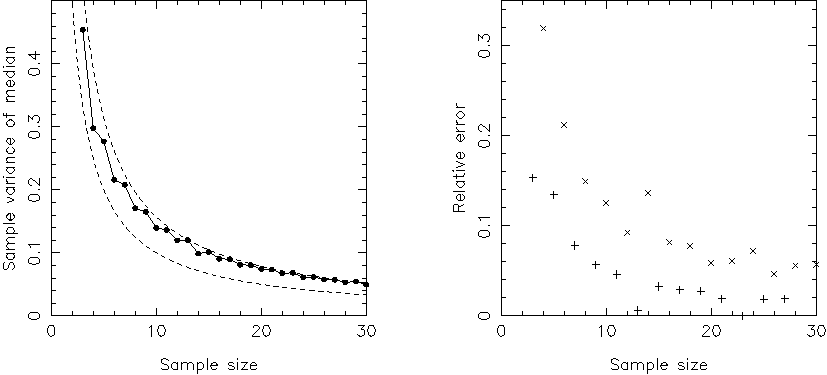
\includegraphics{figures/median_variance}}
  \caption{Sample variance of the median as a function of sample size
    (left panel). The lower dashed curve is the expected variance of
    the arithmetic mean, the upper dashed curve the asymptotic
    variance of the median. The right panel shows the relative error
    compared to the asymptotic variance. Crosses are for even sample
    sizes, pluses for odd sample sizes.}
  \label{fig:median_variance}
\end{figure}

While the sample distribution of the median (which is not Gaussian)
can be written down easily, the computation of its moments and hence
its variance is difficult. A scheme to compute it analytically has
been described in \cite{Maritz-Jarrett1978} and exact values for a few
sample sizes and a number of parent distributions are given in
\cite{Rider1960}. However, these are hardly useful for practical
purposes. The asymptotic value for the ratio of the variances of mean
and median (the \textit{asymptotic relative efficiency} of the median,
\cite{DasGupta2008}) in the Gaussian case is
\begin{equation}
  \label{eq:medvar:asympt}
  \sigma^{2}_{\mathrm{med}} = \frac{\pi}{2}\sigma_{\mathrm{av}}^{2} =
  \frac{\pi\sigma^{2}}{2N}. 
\end{equation}
In Fig.~\ref{fig:median_variance}, we determine the variance of the
median from simulations by drawing for any given sample size $10\,000$
samples from a standard normal distribution. The asymptotic value is
approached from below, which makes it a conservative choice for an
estimate of the median's variance. The relative error, defined as
\begin{equation}
  \label{eq:medvar:asympt:error}
  \frac{\pi/2N - \hat\sigma^{2}_{\mathrm{med}}}{\pi/2N}\,,
\end{equation}
is plotted in the right hand panel of Fig.~\ref{fig:median_variance}. 
For even sample sizes, the relative error is significantly larger than
for odd sizes because the variance is actually lower. For odd-sized
samples, the error is below 10\% for $N\geq7$ ($N\geq 5$
according to \cite{Rider1960}), whereas for even sized samples this
threshold is not crossed until $N\gtrsim 12$. However, as mentioned
above, the asymptotic value in Eq.~(\ref{eq:medvar:asympt}) is
conservative for any $N$ and it is therefore used. 

When each image has its own noise image $\sigma_{i}^{2}(x,y)$
(heteroscedastic case), then a weighted median can be defined as the
point where cumulative weights is equal to $1/2$. Specifically, the
weighted median of an ordered sample of $N$ values $x_{i}$ with
weights $w_{i}$ is 
\begin{align}
  \label{eq:weighted_median}
  x_{\mathrm{wmed}} =
  \begin{cases}
    \displaystyle\frac{x_{j} + x_{j+1}}{2},  &\text{if}\quad
    \sum_{i=1}^{j} w_{i} = 0.5 \\
    \,x_{j},&\text{if}\quad \sum_{i=1}^{j} w_{i} >
    0.5 \quad\text{and}\quad \sum_{i=1}^{j-1} w_{i}< 0.5 
  \end{cases}
\end{align}


\subsection{Kappa-sigma clipping}
\label{sec:algorithms:robust:kappa-sigma}

In the min-max rejection algorithm, a fixed number of sample values
are rejected, regardless whether they can be identified as outliers or
not. If one wants to retain all ``good'' sample values and only reject
true outliers, one has to employ an adaptive method which compares
each sample value to the distribution of the entire sample.

In the $\kappa\sigma$~clipping algorithm, all values that deviate from
the mean by more than $\kappa$ standard deviations are rejected as
outliers. Typically, $\kappa=3$. The mean is usually estimated from
the data, as is the standard deviation if no independent error
estimate is available. One can introduce an iteration which stops once
no more values are rejected. 

Standard $\kappa\sigma$~clipping is not very efficient in removing
low-significance outliers because the estimates of the mean and the
standard deviation are themselves affected by the outliers. Using more
robust estimators of location and scale, like the median and the
inter-quartile range (IQR) or the median absolute deviation (MAD),
improves the situation and makes $\kappa\sigma$~clipping a robust and
easy-to-use adaptive outlier-rejection algorithm. The \HDRL
implementation uses the median and the MAD as robust estimators for
the location and scale.  For a Gaussian distribution, the standard
deviation $\sigma$ is given in terms of the MAD through
\begin{equation}
  \label{eq:sigma-MAD}
  \sigma = \mathrm{MAD} \times 1.4826.
\end{equation}

$\kappa\sigma$~clipping has one parameter, the clipping threshold
$\kappa$. The value of $\kappa$ is not critical if outliers are
expected to lie far from the sample distribution, as is the case for
cosmic ray hits. Weaker effects, such as satellite trails, may require
fine-tuning of $\kappa$.

The functions that make use of $\kappa\sigma$~clipping have a second
parameter, e.g.  \lstinline{niter} which specifies the maximum number
of iterations to run.

The method might fail if more than half of the input images are
affected by outliers at a given pixel because then the estimate of the
MAD might be affected and cause outlier rejection to fail. The method
also requires a sufficient number of input images to be able to obtain
reasonably accurate estimates of the mean and standard deviation.

The variance of the estimator now varies from pixel to pixel depending
on the number of values that are rejected as outliers. Since outliers
are not drawn from the same distribution as the ``good'' data values,
the cleaned sample is equivalent to a smaller sample drawn from the
noise distribution. In the general heteroscedastic case, the variance
is therefore estimated as
\begin{equation}
  \label{eq:ksigma:variance}
  \sigma_{\kappa\sigma}^{2} = \frac{1}{N_{\mathrm{good}}^{2}}
  \sum_{\mathrm{good}} \sigma_{i}^{2}\,.
\end{equation}

\subsection{Mode}
\label{sec:algorithms:robust_mean:mode}

The mode (or modal value) of a distribution of values is defined as
the value of the distribution that appears more often (the maximum of
the function distribution). The \HDRL implements the mode computation
for the case of a discrete distribution.

In the case of a discrete distribution, one can define the ``modal
class'' (the position of the highest peak of the histogram), and the
``modal frequency'' (the value of the highest peak of the histogram),
which are related to the mode of the underlying continuous
distribution.  The value of the modal frequency depends from the
chosen bin size used to create the histogram and from statistical
noise. A large bin size helps in finding a high and unique modal
frequency, but decreases the resolution. A small bin increases the
resolution of the modal class but decreases the modal frequency and
therefore increases the chance that, because of the statistical noise,
the highest peak in the histogram is not related to the mode of the
underlying distribution.

Concerning the determination of the error associated to the mode estimator,
the mode method is special as HDRL
\textbf{calculates the error from the data}
and is not doing pure \textbf{error propagation} as all the
other statistical estimators listed above.
The error calculation depends on the parameter
\verb+error_niter+. If the parameter is set to 0, HDRL estimates the error 
analytically as described below. If the parameter is
larger than 0, the error is calculated by a bootstrap Montecarlo
simulation from the input data with the value of the parameter
specifying the number of simulations. In this case the input data are
perturbed with the bootstrap technique \verb+error_niter+ times and
the mode is derived for each simulation. From this modes the standard
deviation is calculated and returned as error.

The \HDRL implementation in the supported case of discrete
distributions depends on the following parameters:

\begin{itemize}
\item \verb+histo_min+: This parameter defines the lower bound of the
  histogram, i.e. the minimum value of the pixels that are used to
  derive the histogram
  \footnote{\label{footnote1}If $\mbox{histo\_min} < \mbox{histo\_max}+$,
  $\mbox{nbin} = \mbox{floor}(\frac{\mbox{histo\_max}-\mbox{histo\_min}}{\mbox{bin\_size}})+1$,
  data points outside the range [histo\_min,histo\_max] are removed and,
    to be consistent with GSL,  \mbox{histo\_min} is kept to the user value and
  $\mbox{histo\_max} = \mbox{histo\_min} + \mbox{nbin} * \mbox{bin\_size}$}.
    Please note that
  if the lower bound (\verb+histo_min+) is set to the same or to a
  higher value than the upper bound (\verb+histo_max+), both
  parameters are automatically determined from the data by taking the
  minimum value for \verb+histo_min+ and the maximum value for
  \verb+histo_max+.
  \footnote{\label{footnote2}If $\mbox{histo\_min} >= \mbox{histo\_max}$,
  the real minimum internally
  used is always $\mbox{histo\_min} - \frac{\mbox{bin\_size}}{2}$}.

    
\item \verb+histo_max+: This parameter defines the upper bound of the
  histogram, i.e. the maximum value of the pixels that are used to
  derive the histogram\footnoteref{footnote1}.
  Please note that if the upper bound (\verb+histo_max+) is set to the same or
  to a lower value than the lower bound (\verb+histo_min+), both parameters
  are automatically determined from the data by taking the minimum
  value for \verb+histo_min+ and the maximum value for
  \verb+histo_max+
  \footnote{\label{footnote3}If $\mbox{histo\_min} >= \mbox{histo\_max}$,
  the real maximum internally
  used is always $\mbox{histo\_max} + \frac{\mbox{bin\_size}}{2}$}.
\item \verb+bin_size+: This parameter defines the size of the histogram
  bin. Please note that if the value is set to value less or equal to 0, the parameter is
  automatically determined from the data.
\item \verb+mode_method+: This parameter defines the method used to
  compute the mode. Currently there are three methods implemented with an enum:
  \begin{itemize}
  \item \verb+HDRL_MODE_MEDIAN+: This method is the most robust method
    and can/should be used for very asymmetric point
    distributions. For more details see below.
  \item \verb+HDRL_MODE_WEIGHTED+: This method can/should be used with
    asymmetric distributions. For more details see below.
  \item \verb+HDRL_MODE_FIT+: This method give accurate results for
    symmetric distributions but is also more likely to fail. For more
    details see below.
  \end{itemize}
\item \verb+error_niter+: This parameter defines the algorithm to
  compute the error of the mode as, contrary to all the other
  implemented statistical estimators, the mode \textbf{calculates the
    error from the data} and not by \textbf{error
    propagation}. Moreover, it is also special in the sense that one
  can choose between an analytical error estimation and one based on a
  bootstrap simulation. If the parameter is set to 0, HDRL is doing an
  analytical error estimation. If the parameter is larger than 0,
  the error is obtained by a bootstrap Montecarlo simulation from
  the input data with the value of the parameter specifying the number
  of simulations. In this case the input data are perturbed with the
  bootstrap technique and the mode is calculated \verb+error_niter+
  times. From this modes the standard deviation is determined and
  returned as error.
\end{itemize}

In details, the implemented algorithm is performing the following
operations:

\begin{enumerate}
\item Pixels marked as bad (bpm) are removed from the input data.
\item HDRL derives/sets the size of the histogram bins (binsize) as
  follows:
  \begin{itemize}
  \item If \verb+bin_size+ is set to 0, then binsize is automatically
    defined as:
   \[
   {\tt binsize} = 2 \cdot 3.49 \cdot \Sigma /{\tt N_{\rm TOT}}^{1/3}
   \]
   where
   \[
   \Sigma = \biggl\{ \begin{array}{ll}
   
    {\tt MAD}(X)/.67449 & {\rm,  if\ {\tt MAD} (X) \ne 0} \\
      {\tt STDDEV}(X)   & {\rm,  if\ {\tt MAD} (X) = 0} \\
   \end{array}
   \]
   and $N_{\rm TOT}$ is the number of elements of $X$. {\tt MAD} is the
   Median Absolute Deviation and {\tt STDDEV} is the Standard Deviation
   (assuming a degree of freedom of 1). The formula above represents
   Scott's rule for determining the binsize of an histogram, multiplied
   by 2 and with {\tt STDDEV} replaced by {\tt MAD}. The use of the {\tt
     MAD} instead of the standard deviation makes the algorithm more
   robust to the presence of outliers. The factor 1/0.67449 is needed to
   convert {\tt MAD} into standard deviation (this is strictly only valid
   for a Gaussian distribution).
   \item If \verb+bin_size+ is larger than 0, then binsize =
     \verb+bin_size+.
  \end{itemize}
\item Builds a histogram, considering only points in X within {\tt
  max} and {\tt min}. Let's define $v_i$ as the position of the lower
  limits of the i-th bin (a.k.a. ``class'') and $h_i$ as the number of
  elements in the $i-th$ bin (a.k.a. ``frequency''). The vectors $v_i$
  and $h_i$ are outputs, $i$ running from 0 to $N-1$ (do not confuse
  $N$ with $N_{\rm TOT}$).
\item Compute the mode $m$ and its error according to the specified
  algorithm - see
  section~\ref{sec:algorithms:robust_mean:mode_fit},
  section~\ref{sec:algorithms:robust_mean:mode_weighted}, and 
  section~\ref{sec:algorithms:robust_mean:mode_median}
\end{enumerate}

\subsubsection{Mode algorithm: HDRL\_MODE\_FIT}
\label{sec:algorithms:robust_mean:mode_fit}

\begin{enumerate}
\item Locate the highest value of $h$. Define the lower limit of the
  modal class, the value of $v$ that corresponds to $h$, i.e. $v_M$
  with $M$ the index of the highest bin. If there are $N$ adjacent
  bins with the same value of $h$ proceed as follows:
  \begin{enumerate}
    \item Take the mean of the indices of the $n$ bins ($i_1, i_2, ..., i_n$) and round it to the closest integer value $i_m$ and define $M=i_m$.
    \item If there are $n$ non-adjacent bins with the same value of $h$,
      identify the subgroup of $m$ adjacent bins with lower $v$ and
      proceed as before.
    \end{enumerate}
  \item Collect ``at most'' 2 bins below $v_M$, and 2 bins above it. Define $x=[v_{M-2},v_{M-1},v_M,v_{M+1},v_{M+2}]$ and 
$y=[h_{M-2},h_{M-1},h_M,h_{M+1},h_{M+2}]$. If $M\leq 0$ or $M\geq N-3$ be conservative, e.g. if $M=0$ then $x = [v_0,v_1,v_2]$.
\item If there are at least three points in x,y, then fit a parabola,
  otherwise the routine will return with an appropriate error code. Define
  the mode as the value that corresponds to the maximum of the
  parabola.  In formulas, if $p(x)=a_0+a_1x+a_2x^2$ is the equation of
  the parabola ($x$ is continuous variable) and $p(x_M)$ is the
  maximum of the parabola, then the mode is $m = x_M+{\tt binsize}/2$.

  The error on the coefficients of the fit can be used to estimate the
  error on the mode.  The position of the maximum of the parabola is
  $x_M=-a_1/ (2 \cdot a_2)$. Its error can be obtained via error
  propagation:
  %\textcolor{red}{
  \[
    \left( \Delta x_M \right)^2 = \left( \frac{\Delta a_1}{2a_2} \right)^2 +\left( \frac{a_1 \Delta a_2}{2a_2^2} \right)^2 + {\rm COVAR\_TERM}
  \]
  COVAR\_TERM is ad additional term due to the fact that variables $a_2$ and $a_1$ are not independent:
  \[
    {\rm COVAR\_TERM} =  2\cdot \frac{-1}{2\cdot a_2} \frac{a_1}{2a_2^2} \cdot Covar(a_2,a_1)
  \]
  $Covar(a_2,a_1)$ is the term of the covariance matrix. The covariance matrix is defined as the inverse of the following matrix (parabolic case):
\[
  \begin{bmatrix}
    \sum w_i        &   \sum w_i x_i    &  \sum w_i  x_i^2 \\
    \sum w_i x_i    &   \sum w_i x_i^2  &  \sum w_i  x_i^3 \\
    \sum w_i x_i^2  &   \sum w_i x_i^3  &  \sum w_i  x_i^4 
  \end{bmatrix}
  \]
  Because we do not consider the errors on the individual points, we can set $w_i = 1$. HDRL actually uses GSL to compute the fit coefficients $a_{i}$, and the associated errors (taking into account of the covariance). 
  %}

\item If the fit does not converge, or the  mode $m$ computed above is more
  than {\tt binsize}/2 outside the maximum bin, HDRL exit with corresponding
  error message.
  In formulas, if
  \[
  \left| v_M+{\tt binsize}/2-m \right| >{\tt binsize}
  \]
  HDRL issues an appropriate error message.
\end{enumerate}


\begin{figure}
\begin{center}\subfigure
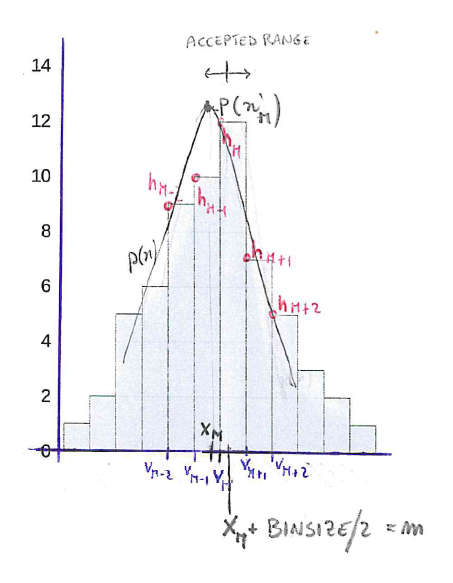
\includegraphics[width=0.4\textwidth]{figures/mode_fig1.jpg}
\caption{Graphic representation of the ``fit'' method to compute the mode of an histogram.}
\label{fig:fit}
\end{center}
\end{figure}
Figure \ref{fig:fit} illustrates the method.


\subsubsection{Mode algorithm: HDRL\_MODE\_WEIGHTED}
\label{sec:algorithms:robust_mean:mode_weighted}

\begin{enumerate}
\item Locate the highest value of $h$. Define the lower limit of the
  modal class, the value of $v$ that corresponds to $h$, i.e. $v_M$ with $M$ the index of the highest bin. If
  there are $N$ adjacent  bins with the same value of $h$ proceed as follows:
  \begin{enumerate}
    \item Take the mean of the indices of the $n$ bins ($i_1, i_2, ..., i_n$) and round it to the closest integer value $i_m$ and define $M=i_m$.
    \item If there are $n$ non-adjacent bins with the same value of $h$,
      identify the subgroup of $m$ adjacent bins with lower $v$ and
      proceed as before.
    \end{enumerate}
 \item If $n$ is even, define  $v'=v_M-{\tt binsize}/2$, if $n$ is odd define $v'=v_M$.

 \item Collect one bin before ($h_0$) and one after ($h_2$) the group
   of $n$ bins with highest value; in formulas
   $v_{M-1-{\rm int}(n/2)}$,$v_{M+1+{\rm int}(n/2)}$, where
   ${\rm int}(n/2)$ is the integer part (if $n=3$ then
   ${\rm int}(n/2)=1$) . Define $f0=h_0$ and $f2=h_2$. If $M=0$ then
$f0=0$. If $M=N-1$ then $f2=0$.

  
 \item Define $d1 = f1-f0$, $d2 =f1-f2 $ and the weight $w=d1/(d1+d2)$.
 \item Define the mode $m=v_M+{\tt binsize}\cdot w$. If $w=0$ or infinite,
   then set $w=0.5$.

  Error on the mode is computed via error propagation, assuming that the errors on d1 and d2 are given by Poisson statistics ($\Delta f_i = \sqrt{f_i}$)
  \begin{eqnarray}
  \Delta d_1 &=& \sqrt{f1+f0} \nonumber \\
  \Delta d_2 &=& \sqrt{f1+f2} \nonumber \\
    \Delta m &=& {\tt binsize}\cdot \Delta w \nonumber \\
\Delta w^2 &=& \left( \frac{d_2\Delta d_1}{(d_1+d_2)^2} \right)^2 + \left( \frac{d_1 \Delta d_2}{(d_1+d_2)^2}\right)^2 
  \end{eqnarray}

\end{enumerate}
Figure \ref{fig:weight} illustrates the method with $n$=1,2, and 3.

\begin{figure}
\begin{center}\subfigure
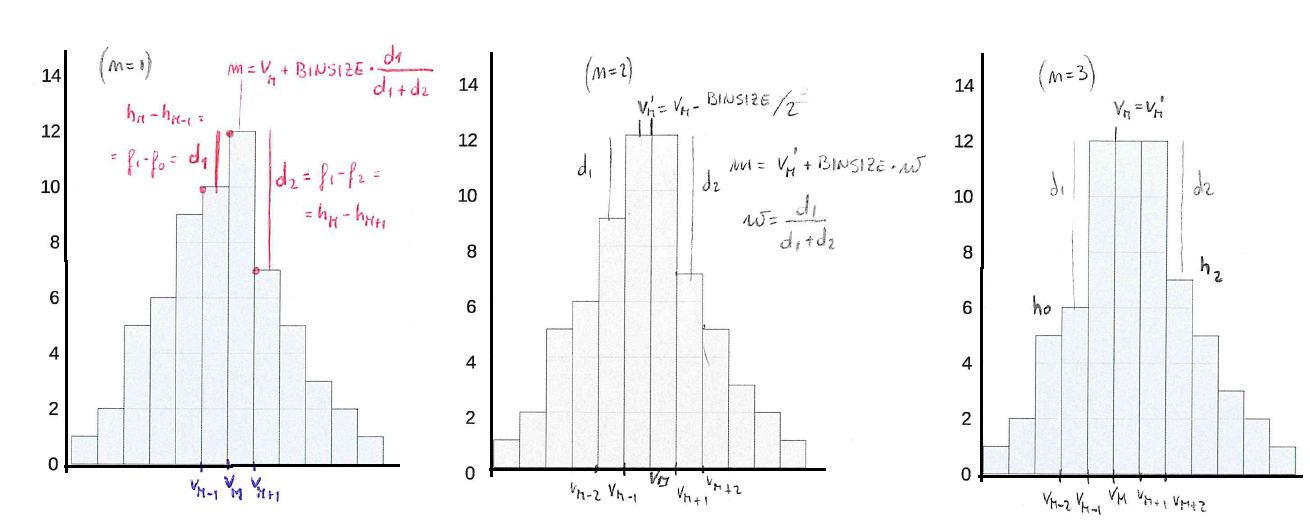
\includegraphics[width=1.05\textwidth]{figures/mode_fig2.jpg}
\caption{Graphic representation of the ``weight'' method to compute
  the mode of an histogram. Three cases are show: single modal class
  (n=1, left panel), two modal classes (n=2, central panel), and three
  modal classes (n=3, right panel).}
\label{fig:weight}
\end{center}
\end{figure}
\subsubsection{Mode algorithm: HDRL\_MODE\_MEDIAN}  
\label{sec:algorithms:robust_mean:mode_median}

This algorithm is suited
for strongly asymmetric distributions (as Gamma distributions).
\begin{enumerate}


\item Locate the highest value of $h$. Define the lower limit of the
  modal class, the value of $v$ that corresponds to $h$, i.e. $v_M$ with $M$ the index of the highest bin. If
  there are $N$ adjacent  bins with the same value of $h$ proceed as follows:
  \begin{enumerate}
    \item Take the mean of the indices of the $n$ bins ($i_1, i_2, ..., i_n$) and round it to the closest integer value $i_m$ and define $M=i_m$.
    \item If there are $n$ non-adjacent bins with the same value of $h$,
      identify the subgroup of $m$ adjacent bins with lower $v$ and
      proceed as before.
    \end{enumerate}

  \item Define the mode as the median of the values of
    $v_M< X <v_M+binsize$. The error on the median is the standard
    deviation of the $X$ values.
    %\textcolor{red}{standard deviation of the $X$ values}.
\end{enumerate}

\section{Bad Pixel Determination}
\label{chap:algorithms:bpm}

\subsection{Detailed Description of the various Algorithms}

%TO BE WRITTEN (SDPG)
%\subsubsection{Bad-pixel detection on a single image}
%TO BE WRITTEN (SDPG)
%\subsubsection{Bad-pixel detection on a stack of images}
%TO BE WRITTEN (SDPG)
%\subsubsection{Bad-pixel detection on a sequence of images}
%TO BE WRITTEN (SDPG)
%
%
%\subsubsection{Cosmic Ray Hits detection}
%
%TO BE WRITTEN (SDPG)
%
%
%\subsection{Performance}
%TO BE WRITTEN (SDPG)

\subsubsection{Bad-pixel detection on a single image}

The {\tt hdrl\_bpm\_2d} recipe identifies bad pixels on individual
images by comparing the value in each pixel with those of the
neighbouring pixels, via two methods.

In method 1 the algorithm first smooths the single image by applying
a cpl-filter (default: median), then subtracts the smoothed images and
derives the bad pixels by scaling the rms with specified thresholds on
the residual image.

Method 2 is similar to method 1, but the smoothed image is obtained
via a Legendre polynomial fit to the image.  More details are given in
Section \ref{sec:bpm_2d}.


We tested the 2 methods on flat fields exposures on sky (both
simulated with artificial bad pixels and real exposures). We found the
following:

\begin{itemize}
\item {\bf Method 1.}  The best performances (missed detections = 0\%,
  false positives = 0\%, recovered bad pixels = 100\%), are obtained
  by setting the recipe parameters to use large smoothing windows
  (i.e. {\tt --bpm.smooth\_ x/y = 49}), relatively high sigma clipping
  levels ({\tt --bpm.kappa\_low/high > 5}), and dilation
  post-filtering with {\tt --pfx/y = 3}. On the contrary, the number of
  false detection increases dramatically. Figure~\ref{fig:single_m1}
  shows the results on simulated flat fields.

\item {\bf Method 2.}  The best performances ($>95$\% success rate)
  are obtained with the sigma clipping levels {\tt
    --bpm.kappa\_low/high = 3}, although this generates a false
  detection rate of 10\%. The number of false detections can be
  lowered by increasing {\tt --bpm.kappa\_low/high}, but but the
  success rate decreases and the number of missed detection increases
  consequentially. The order of the fitting polynomial surface has no
  strong impact on the performances. Figure~\ref{fig:single_m2} shows
  the results on simulated flat fields.

\end{itemize}


\begin{figure} 
 \subfigure
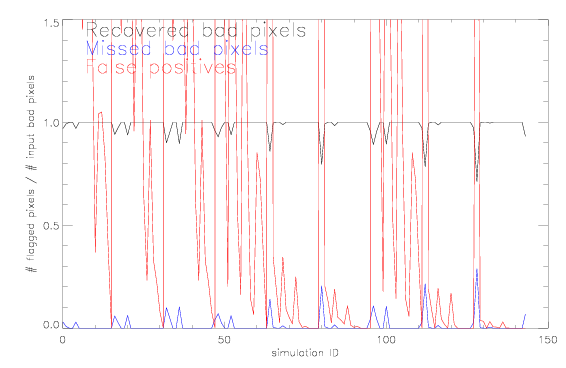
\includegraphics[width=17cm]{figures/recovered_bad_pixels_m1.png}
 \caption{Fraction of recovered bad pixels (black), missed bad pixels
   (blue) and false detections (red) on simulated flat fields using
   method 1 of the {\tt hdrl\_bpm\_2d} recipe. The best performances
   are obtained setting {\tt --bpm.smooth\_x/y =49}, {\tt
     --bpm.kappa\_low/high > 5}, and {\tt --pfx/y =3}. A large
   fraction of false detection is found for {\tt --bpm.smooth\_ x/y
     <5} (corresponding to the run ID that have peaks in the red curve
   in the above figure).}
\label{fig:single_m1}
\end{figure}


\begin{figure}
 \subfigure
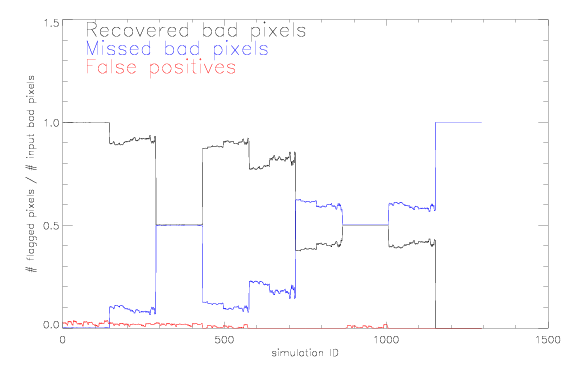
\includegraphics[width=17cm]{figures/recovered_bad_pixels_m2.png}
 \caption{Fraction of recovered bad pixels (black), missed bad pixels
   (blue) and false detections (red) on simulated flat fields using
   method 2 of the {\tt hdrl\_bpm\_2d} recipe. The best performances
   are obtained setting {\tt --bpm.kappa\_low/high = 3} (run ID $<
   100$). For larger values, the number of detected bad pixels
   decreases.}
\label{fig:single_m2}
\end{figure}



\subsubsection{Bad-pixel detection on a stack of images}

The {\tt hdrl\_bpm\_3d} recipe identifies bad pixels on a stack of
images. It compares the value in each pixel of the image $i$-th, with
the same pixel in the other $N-1$ images. It returns a $N$ bad pixel
map cube, with the 3rd axis of dimension $N$.

It has 3 methods, which are detailed in Section ? In a nutshell: 

Method 1 identifies bad pixels using an absolute threshold on
the residual images. The threshold depend strongly on the input data,
and needs to be fine tuned case by case in order to select the best
parameters.

Method 2 identifies bad pixels using a threshold on scaled rms. Method
3 identifies bad pixels by scaling the propagated error of each
individual pixel and compares it with the measured residuals.

Method 2 and 3 have been tested on simulated bias and simulated flat
fields. Both methods have a success rate $> 99$\% in identifying the
bad pixels. Method 3 tends to miss 50\% of the bad pixels if
{\tt --bpm.kappa $\geq$ 10} (method 2 does not have this problem on
the same images), whereas method 2 has a $\sim 6$\% false detection
rate on noise images (method 3 does not have this problem on the same
images).

Figures \ref{fig:stack_m2} and \ref{fig:stack_m3} show the tests on
methods 2 and 3 on noiseless simualted stack of flat fields.


\begin{figure}
 \subfigure
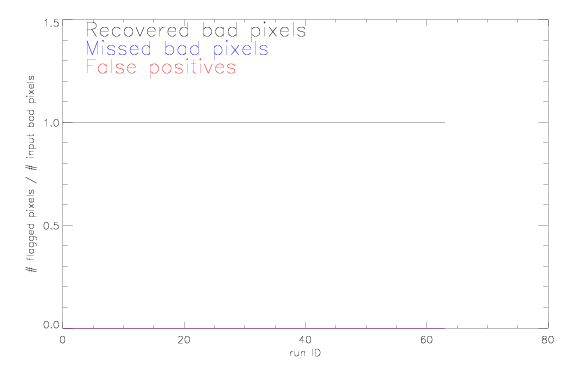
\includegraphics[width=17cm]{figures/recovered_bad_pixels_3d_m2.png}
 \caption{Fraction of recovered bad pixels (black), missed bad pixels
   (blue) and false detections (red) on simulated flat fields, using method 2 of the {\tt hdrl\_bpm\_3d} recipe.}.
 \label{fig:stack_m2}
\end{figure}


\begin{figure}
 \subfigure
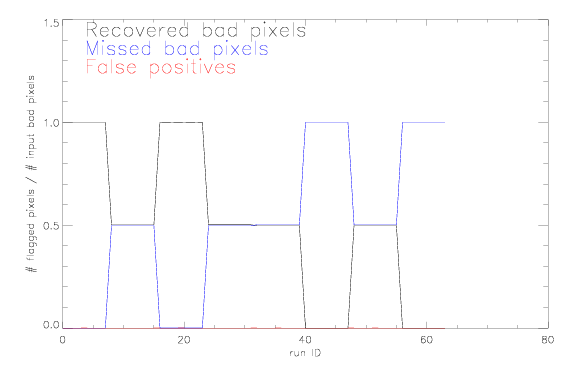
\includegraphics[width=17cm]{figures/recovered_bad_pixels_3d_m3.png}
 \caption{Fraction of recovered bad pixels (black), missed bad pixels
   (blue) and false detections (red) on simulated flat fields, using
   method 3 of the {\tt hdrl\_bpm\_3d} recipe. 50\% of input bad pixels are missed
   if {\tt --bpm.kappa\_low/high > 10}.}
\label{fig:stack_m3}
\end{figure}



\subsubsection{Bad-pixel detection on a sequence of images}

The {\tt hdrl\_bpm\_fit} recipe is targeted to the analysis of a set
of $N$ frames with different exposure time (e.g.  dome flats). At each
position $(x, y)$, bad pixels in each frame are identified via a
polynomial fit of all the $N$ pixels at position $(x, y)$. The header
keyword {\tt EXPTIME} is used as to sampling position of the $N$
pixels along the fit.


{\it Warning}: the routine does not disentangle between i) bad pixels
or non-linear pixel (i.e. ``persistent'' bad values of the same pixel
across the stack of images) and ii) ``accidental'' bad pixel values
(i.e.  the pixel itself is good, but in one frame it has a deviant
value because, for example, of a cosmic ray event). If a pixel in the
sequence of images is flagged in one frame (e.g. a cosmic ray hit it)
but it is not on the other frames, it is flagged in the final mask.

It is therefore advisable to remove cosmic rays on individual frames,
before running {\tt hdrl\_bpm\_fit} on a sequence of images.


The  {\tt hdrl\_bpm\_fit}  recipe has 4 methods:

\begin{itemize}
\item {\bf Method 1.} ({\tt --abs-rchi2-low/-high}): This method marks pixels
  as bad by using the absolute reduced chi squared (low/high)
  threshold: pixels with values below/above this threshold are marked
  as bad. This method needs to be fine-tuned for each dataset, because
  it refers to absolute chi2 values.
                                                                             
\item {\bf Method 2.} ({\tt --rel-rchi2-low/-high}): This method marks
  pixels as bad by using the relative reduced-chi-squared (low/high)
  threshold: pixels with values below/above this threshold times
  measured-rms are marked as bad.
                                                                             
\item {\bf Method 3.} ({\tt --rel-coef-low/-high}): This method marks pixels
  as bad by using the relative coefficient (low/high) threshold:
  pixels with values below/above this threshold times measured-rms are
  marked as bad.
                                                                             
\item {\bf Method 4.}  ( {\tt --pval}): This method uses the p-value
  (between 0\% and 100\%) to discriminate between good and bad pixels.
  Fits with a p-value below the threshold are considered to be bad
  pixels.

\end{itemize}

Figures~\ref{fig:sequence_m2}, \ref{fig:sequence_m3}, and
\ref{fig:sequence_m4} show the results of tests performed on a
sequence of simulated flat fields. Method 2 and 3 tend to miss a large
fraction of bad pixels for {\tt --rel-rchi2} and {\tt --rel-coef}
larger than 1 (which correspond to the first run ID in the mentioned
figures).  Method 4 gives the best performances, independently of the
input {\tt --pval} value.

\begin{figure}
 \subfigure
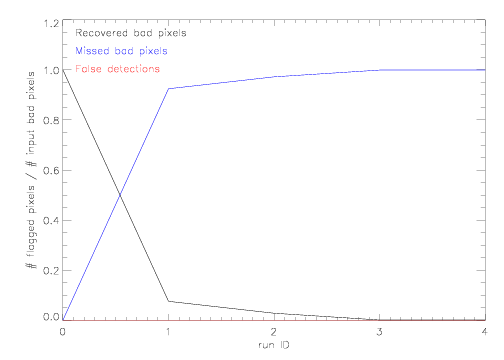
\includegraphics[width=15cm]{figures/results_2.png}
 \caption{Fraction of recovered bad pixels (black), missed bad pixels
   (blue) and false detections (red) on simulated flat fields, using
   method 2 (--rel-rchi2) of the {\tt hdrl\_bpm\_fit} recipe. The best
   performance (run ID=0) corresponds to {\tt --rel-rchi2 = 1}.}
 \label{fig:sequence_m2}
\end{figure}


\begin{figure}
 \subfigure
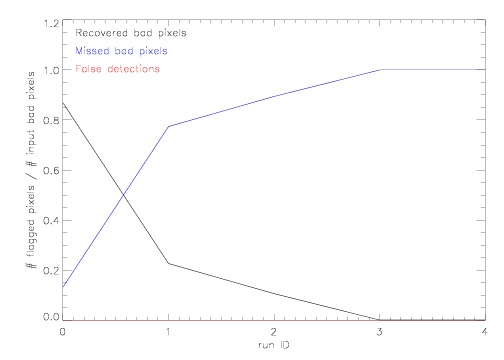
\includegraphics[width=15cm]{figures/results_3.png}
 \caption{Fraction of recovered bad pixels (black), missed bad pixels
   (blue) and false detections (red) on simulated flat fields, using
   method 3 (--rel-coef) of the  {\tt hdrl\_bpm\_fit}  recipe. The best
   performance (run ID=0) corresponds to {\tt --rel-coef = 1}.}
 \label{fig:sequence_m3}
\end{figure}


\begin{figure}
 \subfigure
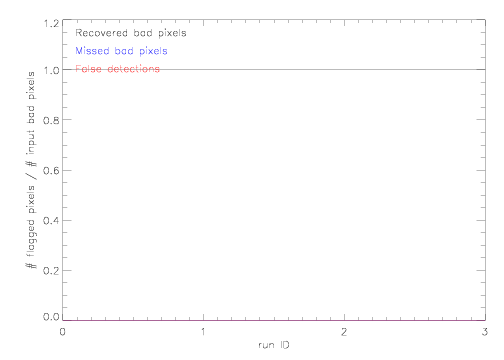
\includegraphics[width=15cm]{figures/results_4.png}
 \caption{Fraction of recovered bad pixels (black), missed bad pixels
   (blue) and false detections (red) on simulated flat fields, using
   method 4 ({\tt --pval}) of the {\tt hdrl\_bpm\_fit} recipe.}
 \label{fig:sequence_m4}
\end{figure}


Driven by robustness of method 4, we tested it on a series of real
flat fields obtained with FORS2 and CRIRES. The test is aimed to
confirm that the number of detected bad pixels is nearly independent
of the adopted {\tt --pval} in {\tt hdrl\_bpm\_fit}. Figure~\ref{fig:sequence_m4_real} indicates indeed
that this is the case: the number of detected bad pixels does not vary
significantly in the range 0.001 < {\tt --pval} < 0.1. Therefore, the defaul
value {\tt --pval = 0.001} can be adopted for most applications.

\begin{figure}
 \subfigure
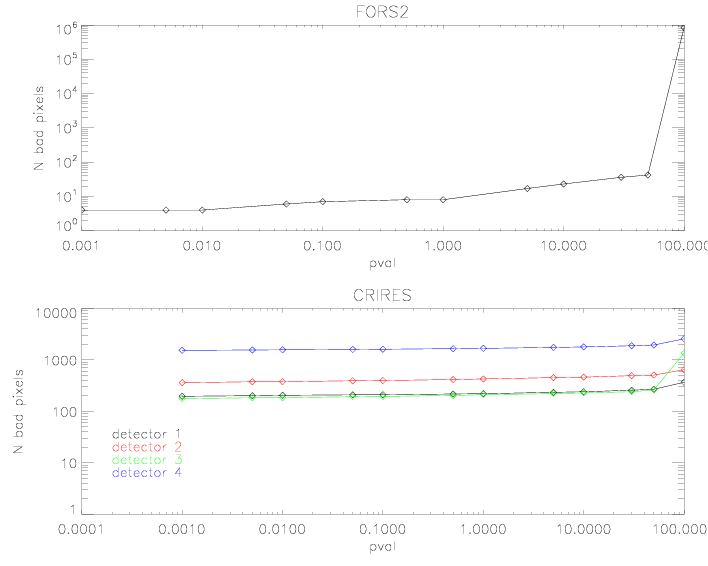
\includegraphics[width=15cm]{figures/results_bpmfit_real.png}
 \caption{Number of flagged bad pixels with {\tt hdrl\_bpm\_fit},
   method 4 as a function of the {\tt --pval} on a series of internal
   flats for FORS2 (upper panel) and CRIRES (lowe panel). The number
   of detected bad pixels does not vary significantly within {\tt
     0.001 < --pval < 0.1}.}
 \label{fig:sequence_m4_real}
\end{figure}


\subsubsection{Cosmic Ray Detection}


The cosmic ray detection algorithm is derived from the LACosmic routine (\cite{vanDokkum2001}).
LACosmic is based on a variation of Laplacian edge detection which uses the sharpness of the
edges of cosmic rays to discriminate between legitimate sources and cosmic rays.   A detailed
description of the algorithm, the default parameters, and applicable data cases
are summarized in \cite{vanDokkum2001}.

In summary, the {\em hdrldemo\_bpm\_lacosmic} routine has the following input parameters:\\

\begin{tabbing}

\quad\= --lacosmic.sigma\_lim\quad  \= structure image that a point must have to be flagged as a cosmic ray. 
\quad \= Default Value Used\kill\\
\> {\bf Parameter}			\>  {\bf Description}					\> {\bf Default Values}       \\
\>  --ext-r                	\>  FITS extension of the RAW. 				\>0      \\
\>  --ext-e               	\>  FITS extension of the ERROR. 				\>0      \\
\>  --ext-b               	\>   FITS extension or the input BPM. 				\>0      \\
\>  --gain                	\>  Gain in [e- / ADU]. 						\>2.5      \\
\>  --ron                 	\>  Read-Out Noise. 							\>1.0      \\
\>  --pfx                 	\>  X Size of the post filtering kernel. 					\>3      \\
\>  --pfy                 	\>   Y Size of the post filtering kernel. 				\>3      \\
\>  --pfm                 	\>   Post filtering mode. [closing or dilation] 				\> closing      \\
\>  --region-llx          	\>   Lower left x pos. (FITS) defining the region. 				\>1      \\
\>  --region-lly          	\>   Lower left y pos. (FITS) defining the region. 				\>1      \\
\>  --region-urx          	\>   Upper right x pos. (FITS) defining the region. 				\>0      \\
\>  --region-ury          	\>  Upper right y pos. (FITS) defining the region. 				\>0      \\
\>  --lacosmic.sigma\_lim  	\>   Poisson fluctuation threshold to flag cosmic rays. 				\>4.5      \\
\>  --lacosmic.f\_lim     	\>   Minimum contrast between the Laplacian image and the fine   \> \\
\>                                   \> structure image that a point must have to be flagged as a cosmic ray.                 \>  2.0 \\
\>  --lacosmic.max\_iter   	\>   Max number of iterations. 				\>5      \\

\end{tabbing}


The User can expect to achieve detection efficiencies of about 90\% on well-sampled images.   This is discussed
in detail in section \ref{sect:testing_CR}.

A good strategy is to run the routine on a typical image using the default parameter values, and then to load the
input image and the resultant cosmic ray detection mask into a display and blink the images.  By slightly varying
the parameters {\em lacosmic.sigma\_lim} and {\em lacosmic.f\_lim} the User can balance the optimal detection
efficiency versus spurious cosmic ray detections.

The detection efficiency and the number of spurious cosmic ray detections can be expected to worsen in data that
is under-sampled.   This may also be true for long slit spectra in which the source spectrum is very sharp.



\subsubsection{Testing the Cosmic Ray Detection}
\label{sect:testing_CR}

The defining parameters of any cosmic ray detection algorithm is its detection efficiency 
(the ratio of the number of cosmic rays found by the routine divided by the total number of cosmic rays), 
the number of spurious detections, and how the total number of cosmic rays and the background environment 
affects the detection.  Therefore, all testing was done by creating a known 
number of cosmic rays of various intensity, size, and shape, and adding these to three different synthetic 
images: an empty field with a Poisson noise distribution, a sparse star and galaxy field, and a dense globular 
cluster field.  The number of cosmic rays was allowed to vary from 50, affecting 300 pixels and covering 0.007\% of 
the field, up to 10,000 cosmic rays, affecting 61,000 pixels and covering 1.5\% of the image.
The recipe was then run on 3 $\times$ 37 = 111 images, stepping between these two extremes of cosmic ray density, and the input cosmic ray 
frames were compared to the detections achieved with the {\em hdrldemo bpm lacosmic} routine. The cosmic ray detection rate was 
a good 89.4\% $\pm$ 0.4\% for the empty and sparse fields, all the way out to unrealistic cosmic ray covering factors of 1.5\%. 
In general, the detection efficiency in the very dense images was, on average, only about 0.3\% worse at a level of 89.1\% $\pm$ 0.4\%. 
The fraction of spurious cosmic ray detections are at a level of about 6.8\% $\pm$ 0.3\% over the full range of cosmic ray densities.

As is evident in figure~\ref{fig:detect_efficiency}, the cosmic ray detection rate is at a level of 
89.4\% $\pm$ 0.4\% for the empty and sparse fields, all the way out to the extremely high cosmic ray covering factors of 1.5\%.   
There is no significant difference in the detection efficiency for the empty images and the sparse fields.
For the very dense images the detection efficiency is not notably worse and is, on average, at a level of 89.1\% $\pm$ 0.4\%.    
The difference between the dense fields and the sparse and empty fields is roughly constant at about 0.3\%.   	
 
Beyond a cosmic ray covering factor of 0.1\%, however, the detection efficiency remains remarkably constant all the way to the 
most densely populated cosmic ray fields.  In this range of covering factors, the number of affected cosmic ray pixels goes 
from 4,000 to 61,000.


\begin{figure}[t]
 \subfigure
\centering
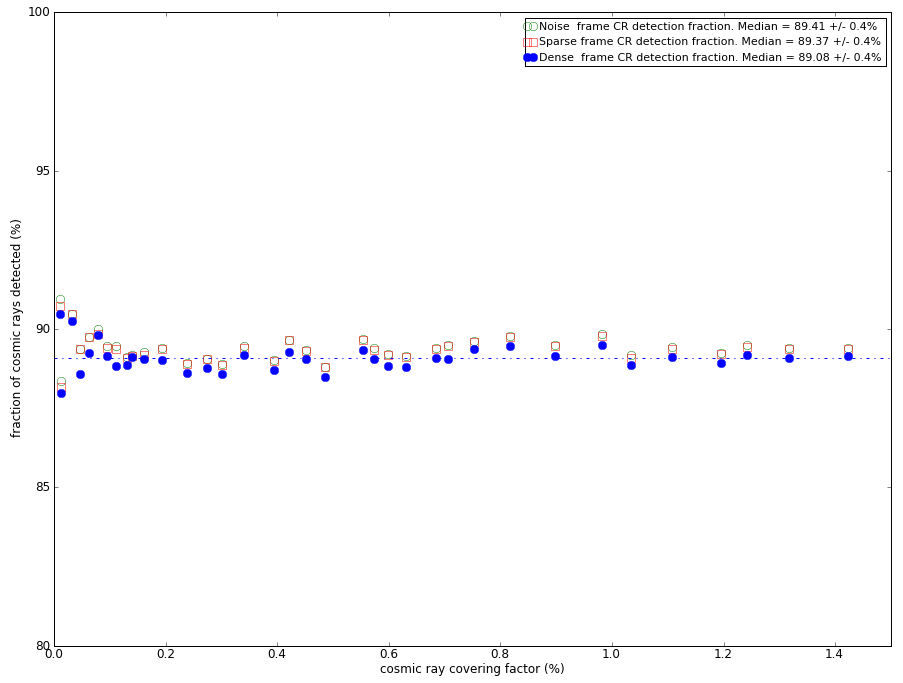
\includegraphics[width=12cm]{figures/LACosmic_det_eff.png} 
%\vspace*{-0.5cm}
\caption[]
	{\footnotesize  The detection efficiency of {\em hdrldemo bpm lacosmic} versus the cosmic ray covering factor (in percent).  The efficiency (given in percent) is measured
	from the number of cosmic rays detected by {\em hdrldemo bpm lacosmic} when applied to the pure noise frame (open green circles), the sparsely populated frame (red squares),
	and the dense frame (solid blue circles).  The average detection rates for the pure background and sparse frames are very similar at 89.4\% $\pm$ 0.4\%, while
	the detection rates in the dense globular cluster frame is always slightly lower at an average of 89.1\% $\pm$ 0.4\%.  The detection efficiency remains remarkably
	constant from cosmic ray covering factors of about 0.1\% to 1.4\% (i.e. from 4,000 to 61,000 affected pixels).
	}
	\label{fig:detect_efficiency}
\end{figure}



The inverse of figure~\ref{fig:detect_efficiency} is given by the fraction of input cosmic rays not detected (see figure~\ref{fig:not_detected}). 
The total count of undetected cosmic rays (figure~\ref{fig:not_detected}, bottom plot) is made independently of the number of detections and is,
therefore, included. Again, for the full range of cosmic ray covering factors, the non-detection rate is about 10.6\% $\pm$ 0.4 for the empty and sparse fields, 
and 11.0\% $\pm$ 0.4\% for the very dense field.

\begin{figure}[b]
 \subfigure
\centering
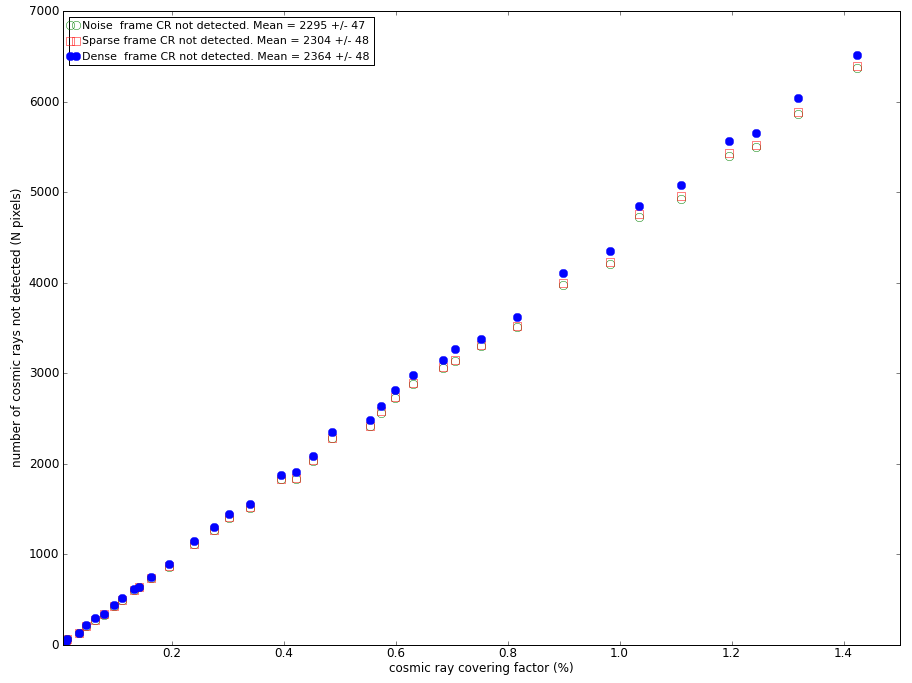
\includegraphics[width=12cm]{figures/LACosmic_not_detA.png} 
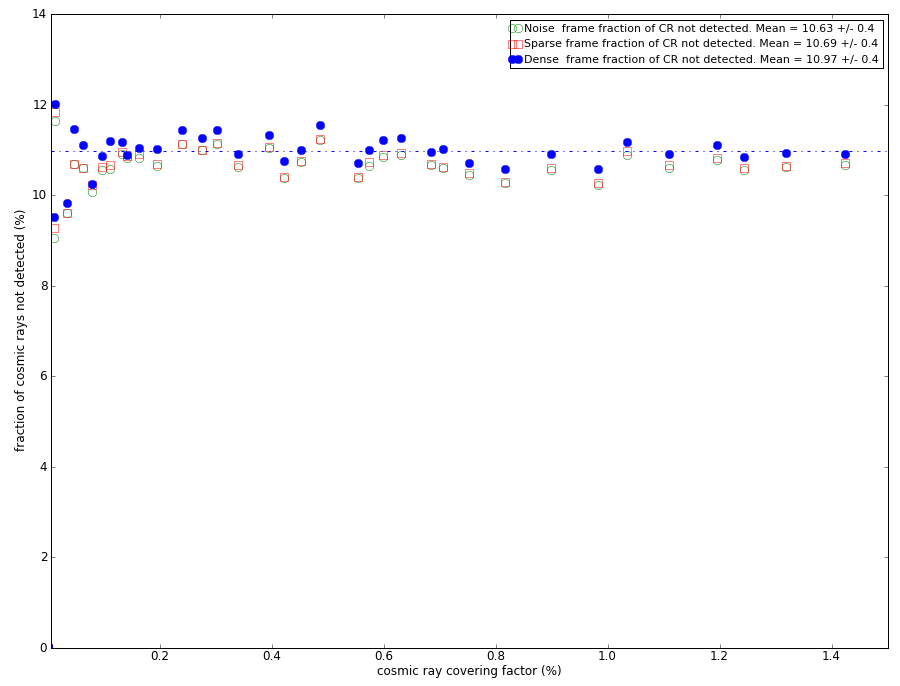
\includegraphics[width=12cm]{figures/LACosmic_not_detB.png}
\caption[]
	{\footnotesize  The number of cosmic rays {\bf not} detected (top panel) and the non-detection fraction (bottom panel) versus the cosmic ray covering factor
	(given in percent).
	}
	\label{fig:not_detected}
\end{figure}


Finally, a count of cosmic rays was made that were detected by {\em hdrldemo bpm lacosmic}, but that do not exist in the original input image (see figure~\ref{fig:spurious}).
The fraction of spurious cosmic ray detections are large for very low covering factors, but this is simply due to the small total numbers
of cosmic rays.   Beyond a covering factor of about 0.2\%, the fraction of spurious cosmic ray detections settles down to a value of about 6.8\% $\pm$ 0.3\%.
Within this regime, the numbers of false-positive detections are virtually indistinguishable between the empty, the sparse, and the dense
fields.

\vspace*{-0.5cm}
\begin{figure}[b]
 \subfigure
\centering
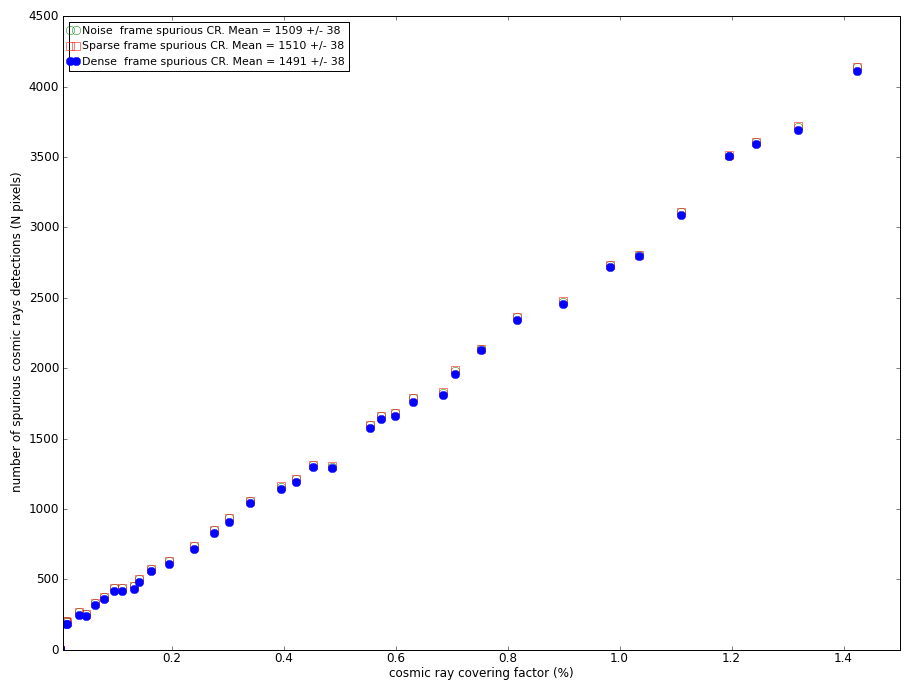
\includegraphics[width=13.3cm]{figures/LACosmic_spuriousA.png} 
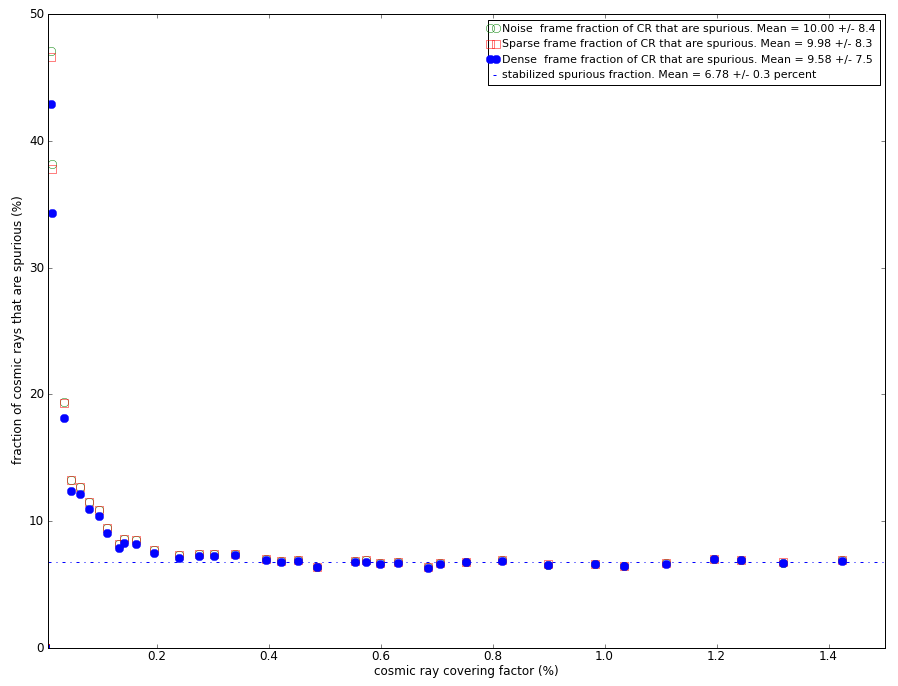
\includegraphics[width=13.3cm]{figures/LACosmic_spuriousB.png}
\caption[]
	{\footnotesize  The number of spurious cosmic ray detections (top panel) and the spurious fraction (bottom panel) versus the cosmic ray covering factor
	(given in percent).
	}
	\label{fig:spurious}
\end{figure}




\section{Masterfringe Computation and Removal}
\label{chap:algorithms:fringing}

\subsection{Detailed Description of the de-fringing Algorithm}
TO BE WRITTEN (SDPG)

\section{Object Catalogue Generation}
\label{chap:algorithms:catalogue}

\subsection{Detailed Description of the Object Catalogue Generation Algorithm}
TO BE WRITTEN (SDPG)
\subsection{Detailed Description of the Object Catalogue Table}
TO BE WRITTEN (SDPG)

\section{Efficiency Calculation}
\label{chap:algorithms:efficiency}

\subsection{Introduction}
In order to determine the efficiency of an instrument (including
telescope and detector) spectrophotometric standard stars are observed
on photometric nights and with setups that collect as much as possible
(e.g. wide slits for slit spectrographs). After correcting for atmopsheric
effects, photon energy, and mirror collecting 
area the ratio between the observed spectrum and the reference
spectrum of the standard star will provide the efficiency of the system.

The observed spectra of the standard
stars are first corrected for atmospheric effects:
\begin{enumerate}
\item The continuous {\em atmospheric extinction} is usually corrected
  with a standard extinction curve obtained for a given observatory,
  scaled with the airmass of the observation. During non-photometric
  conditions the actual extinction may be higher than the one
  tabulated in the extinction curve. The impact of this correction
  decreases with increasing wavelength. 
\item Wavelength above about 600\,nm\footnote{Ozone absorption affects
    the bluest part of ground-based data at about 310--330\,nm, but these are
    noticeable only in high S/N data.} are affected by {\em telluric
    absorption lines}. If these are not corrected the efficiency
  will contain a mixture of instrument response and atmospheric
  response, especially if the reference spectra are free from telluirc
  lines (space-based data or model spectra). Reference spectra for
  many standard stars used for ESO instruments (e.g. UVES, FORS2,
  VIMOS) contain telluric lines
  (e.g. \cite{Hamuy+92,Hamuy+94}). For such reference spectra a
  telluric correction of the observed spectra is useless and one
  should instead interpolate the efficiency across the regions of
  significant telluric absorption.
\end{enumerate}

Possibly the wavelength scale between the observed standard star
spectrum and the reference one needs to be aligned, either to correct
differences in radial velocity between the observed and the reference
spectrum in case of model spectra (e.g. X-shooter, SINFONI) and/or to
correct shifts introduced by imprecise positioning of the flux
standard star in the slit (e.g. VIMOS). If the differences in
wavelength become significant for a given resolution the division of
the reference spectrum by the observed one will create pseudo-P\,Cyg
prodiles, which may distort the efficiency.

These requirements results in the algorithmic steps described in
Sect.\,\ref{efficiency:main}.

\subsection{Testing}
Once the response determination has been implemented in HDRL and
incorporated in the SINFONI pipeline QCG tested it by comparing the
resulting values to the SPIFFI commissioning report
(VLT-TRE-MPE-14720-8003) and found good agreement. The efficiency is
trended at \url{http://www.eso.org/observing/dfo/quality/SINFONI/reports/HEALTH/trend_report_EFFICIENCY_HC.html}

\section{Response Calculation}
\label{chap:algorithms:response}
\subsection{Introduction}
In order to determine the spectroscopic response of an instrument (including
telescope and detector) spectrophotometric standard stars are observed
with the same setup as the science targets\footnote{For slit
  spectrrographs one generally uses a wide slit for flux standard
  stars to capture all flux.}. Spectrophotometric standard stars are
preferably observed during photometric conditions to reduce the
importance of atmospheric effects. After correcting for atmopsheric
effects the ratio between the reference spectrum of the standard star
and the observed spectrum will provide the response of the system.

If the science and/or standard star
data are observed during non-photometric conditions an absolute flux
calibration is impossible. For slit spectra the use of a narrow slit
introduces slit losses that are hard to correct. In many cases,
however, only a {\em relative} flux calibration is required, namely a
response curve that allows the user to correct the observed science
data for bumps and wriggles that were not corrected by the flat
fielding process.

The observed spectra of the standard
stars are first corrected for atmospheric effects:
\begin{enumerate}
\item The continuous {\em atmospheric extinction} is usually corrected
  with a standard extinction curve obtained for a given observatory,
  scaled with the airmass of the observation. During non-photometric
  conditions the actual extinction may be higher than the one
  tabulated in the extinction curve. The impact of this correction
  decreases with increasing wavelength. 
\item Wavelength above about 600\,nm\footnote{Ozone absorption affects
    the bluest part of ground-based data at about 310--330\,nm, but these are
    noticeable only in high S/N data.} are affected by {\em telluric
    absorption lines}. If these are not corrected the response curve
  will contain a mixture of instrument response and atmospheric
  response, especially if the reference spectra are free from telluirc
  lines (space-based data or model spectra). Reference spectra for
  many standard stars used for ESO instruments (e.g. UVES, FORS2,
  VIMOS) contain telluric lines
  (e.g. \cite{Hamuy+92,Hamuy+94}). For such reference spectra a
  telluric correction of the observed spectra is useless and one
  should instead interpolate the response across the regions of
  significant telluric absorption.
\end{enumerate}

Possibly the wavelength scale between the observed standard star
spectrum and the reference one needs to be aligned, either to correct
differences in radial velocity between the observed and the reference
spectrum in case of model spectra (e.g. X-shooter, SINFONI) and/or to
correct shifts introduced by imprecise positioning of the flux
standard star in the slit (e.g. VIMOS). If the differences in
wavelength become significant for a given resolution the division of
the reference spectrum by the observed one will create pseudo-P\,Cyg
prodiles, which will distort the response.

These requirements results in the algorithmic steps described in
Sect.\,\ref{response:main}.

\subsection{Testing}
Once the response determination has been implemented in HDRL and
incorporated in the SINFONI pipeline we tested it by calibrating one
standard star with the response curve from another (observed with the
same setup, but not necessarily during the same night). From the
resulting cube we extracted the one-dimensional spectrum with {\tt
  QFitsView} (using a radius of 11 pixels and {\tt sum}) and corrected
it with a background spectrum extracted with the same aperture. The
difference of the two spectra was then compared to the reference flux
for the standard star. Figures \ref{fig:Feige110_J},
\ref{fig:LTT7987_K}, and \ref{fig:Feige110_HK} show example
results. Due to the small number of observations only limited tests
were possible, which showed no problems that cannot be explained by
transparency differences between the observations of the standard stars.
 
\begin{figure}[H]
\centering \subfigure
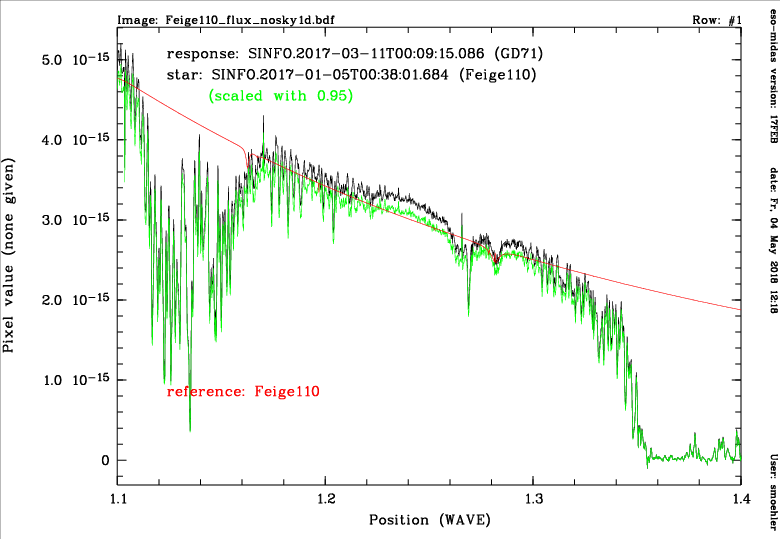
\includegraphics[width=16cm]{figures/Feige110_J.png} 
\caption[]
	{\footnotesize  The {\tt J} spectrum of the flux standard stars
          Feige\,110 calibrated with a response curve from the flux
          standard star GD\,71. The two stars were observed about 2
          months apart on nights of unknown quality. Scaling the
          flux-calibrated spectrum of Feige\,110 by 95\% achives good
          agreement with its reference data.}
	\label{fig:Feige110_J}
\end{figure}

\begin{figure}[H]
\centering \subfigure
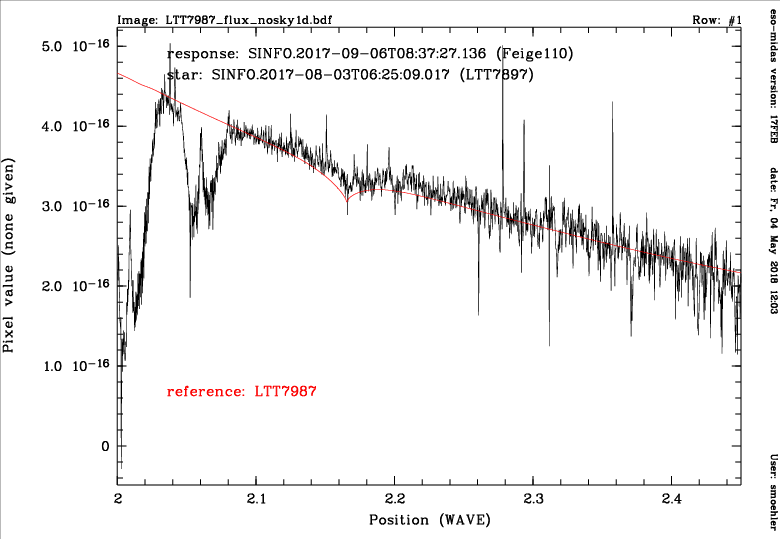
\includegraphics[width=16cm]{figures/LTT7987_K.png} 
\caption[]
	{\footnotesize  The {\tt K} spectrum of the flux standard stars
          LTT\,7987 calibrated with a response curve from the flux
          standard star LTT\,7987. The two stars were observed about 1
          month apart on nights of unknown quality. Nevertheless the
          flux-calibrated spectrum of LTT\,7987 agrees well with its
          reference data.} 
	\label{fig:LTT7987_K}
\end{figure}

\begin{figure}[H]
\centering \subfigure
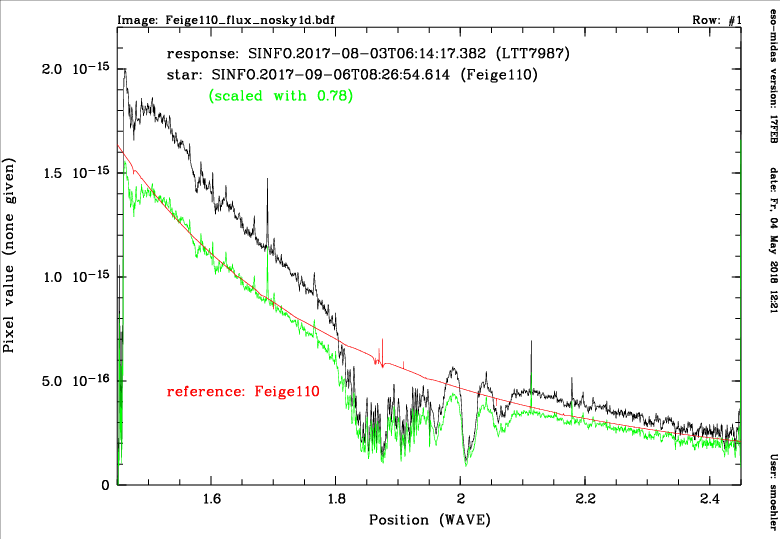
\includegraphics[width=16cm]{figures/Feige110_HK.png} 
\caption[]
	{\footnotesize  The {\tt H+K} spectrum of the flux standard stars
          Feige\,110 calibrated with a response curve from the flux
          standard star LTT\,7987. The two stars were observed about 1
          month apart on nights of unknown quality. Scaling the
          flux-calibrated spectrum of Feige\,110 by 78\% achives good
          agreement with its reference data.}
	\label{fig:Feige110_HK}
\end{figure}

\section{Differential Atmospheric Refraction}
\label{chap:DAR}

\def\hdrldar{{\em hdrl\_dar}}
\def\hdrlcat{{\em hdrl\_catalogue}}
\def\hdrlstrehl{{\em hdrl\_strehl}}



\subsection{Introduction}

The effects of atmospheric refraction can be readily seen in any spectrograph or IFU. Atmospheric refraction will displace a source, or its spectrum, 
by an amount that is dependent on the source wavelength and the angular distance of the source from the zenith.  
This effect is due to the stratified density structure of our atmosphere, and the displacement will be toward the zenith and will be largest for shorter wavelengths.
Because of this latter attribute, differential atmospheric refraction is not generally associated with infrared instruments. However, it can be 
readily seen in SINFONI data cubes observed with the largest wavelength coverage (H+K) and in the smallest pixel scales (25 mas). 
Here, the shift can be as large as 6 pixels from the beginning of the data cube to its end (see Figures \ref{fig:SINFONI_trace} and \ref{fig:SINFONI_image}).

This module uses an analytical approach to compute the expected differential refraction as a function of wavelength, zenith angle, and the refractive index of air
which, in turn, depends on temperature, pressure, and water vapour pressure.

The \hdrldar\ routines require the following inputs (all of which are, generally, available in the input data headers):
\begin{itemize}
\item the ambient atmospheric parameters: temperature, pressure, and humidity as contained in the environmental keyword headers:
TEL.AMBI.TEMP, TEL.AMBI.PRES.START/END, and TEL.AMBI.RHUM, respectively.
\item the instrument rotation angle on the sky
\item the parallactic angle of instrument
\item and, the world-coordinate system (WCS)
\end{itemize}


\subsection{Testing HDRL DAR}
\label{chap:testing_DAR}

The goal of this test series is to compare the actual source displacements, as measured in processed SINFONI
data cubes, with the displacements predicted by \hdrldar.

SINFONI standard stars were selected for this comparison as they tend to be bright, display some flux for the full
wavelength range covered, and are point sources.   The standard star data was selected from the ESO archive for the years 2014, 2015, and 2016.  
Furthermore, this data was selected to cover the $J$ and $H + K$-bands as they are most susceptible to 
atmospheric refraction; the former because it is the bluest filter, and the latter because it covers the 
largest span in wavelength. Data from all three SINFONI image scales was used. In order to test the full range 
of parameters relevant to atmospheric refraction, an effort was made to ensure that the data covered a 
significant range of instrument rotation angles, airmasses, air pressures, temperatures, and relative humidities
(see Table \ref{fig:SINFONI_data}).

\begin{table}[ht]
\caption{Parameter Ranges Covered by SINFONI Data}
\begin{center}
\begin{tabular}{ l c c }
{\bf SINFONI Cube Parameter}			& \multicolumn{2}{l}{{\bf Range of Parameters}}  \\
  								& {\bf Minimum}	& {\bf Maximum} \\
 instrumental rotation angle [degrees]	& -230			& 234.2	   \\				
 airmass [degrees] 					& 1.001			& 2.350	   \\
 air pressure [HPa]                 			& 739.5   			& 747.8     \\
 temperature [$^\circ$C]      			& 3.4				& 20.0       \\
  relative humidity [\%]             			& 3.0    			& 63.0 	   \\
\end{tabular}
\end{center}
\label{fig:SINFONI_data}
\end{table}

The standard star data was processed using the SINFONI pipeline version 3.0.0 running as a Reflex workflow.  All processing parameters were left
in their default values.   In total, 754 SINFONI data cube products were created in this processing.    

\subsection{Testing the \hdrldar\ Differential Atmospheric Refraction Routines with SINFONI Data}

\subsubsection{I.  Method and Qualitative Results}

For each SINFONI data cube, a source centroid for each cube plane (omitting the first and last 100 planes due to higher noise levels) was computed, in order to measure
the actual source shifts due to atmospheric refraction.  This is done using the source detection catalogue routines (\hdrlcat) adapted from CASU (Madsen, G.,   
HAWK-I Pipeline User Manual, February 19, 2016.  Issue 1.0.).
For each of the 754 data cubes analysed, plots were created mapping the measured source centroids ($X_c$ and $Y_c$) as a function of wavelength through the data cube.    
For each of these source traces, the shift values computed by the \hdrldar\ output tables were applied to the centroids to correct the
differential atmospheric refraction.  A typical example of such a trace is shown in Figure \ref{fig:SINFONI_trace}.
A comparison of the median-collapsed cube images before and after being corrected for atmospheric refraction (at an integer shift level) is shown in Figure \ref{fig:SINFONI_image}.
In both plots, a significant qualitative improvement is apparent.

\begin{figure}[H]
\centering \subfigure
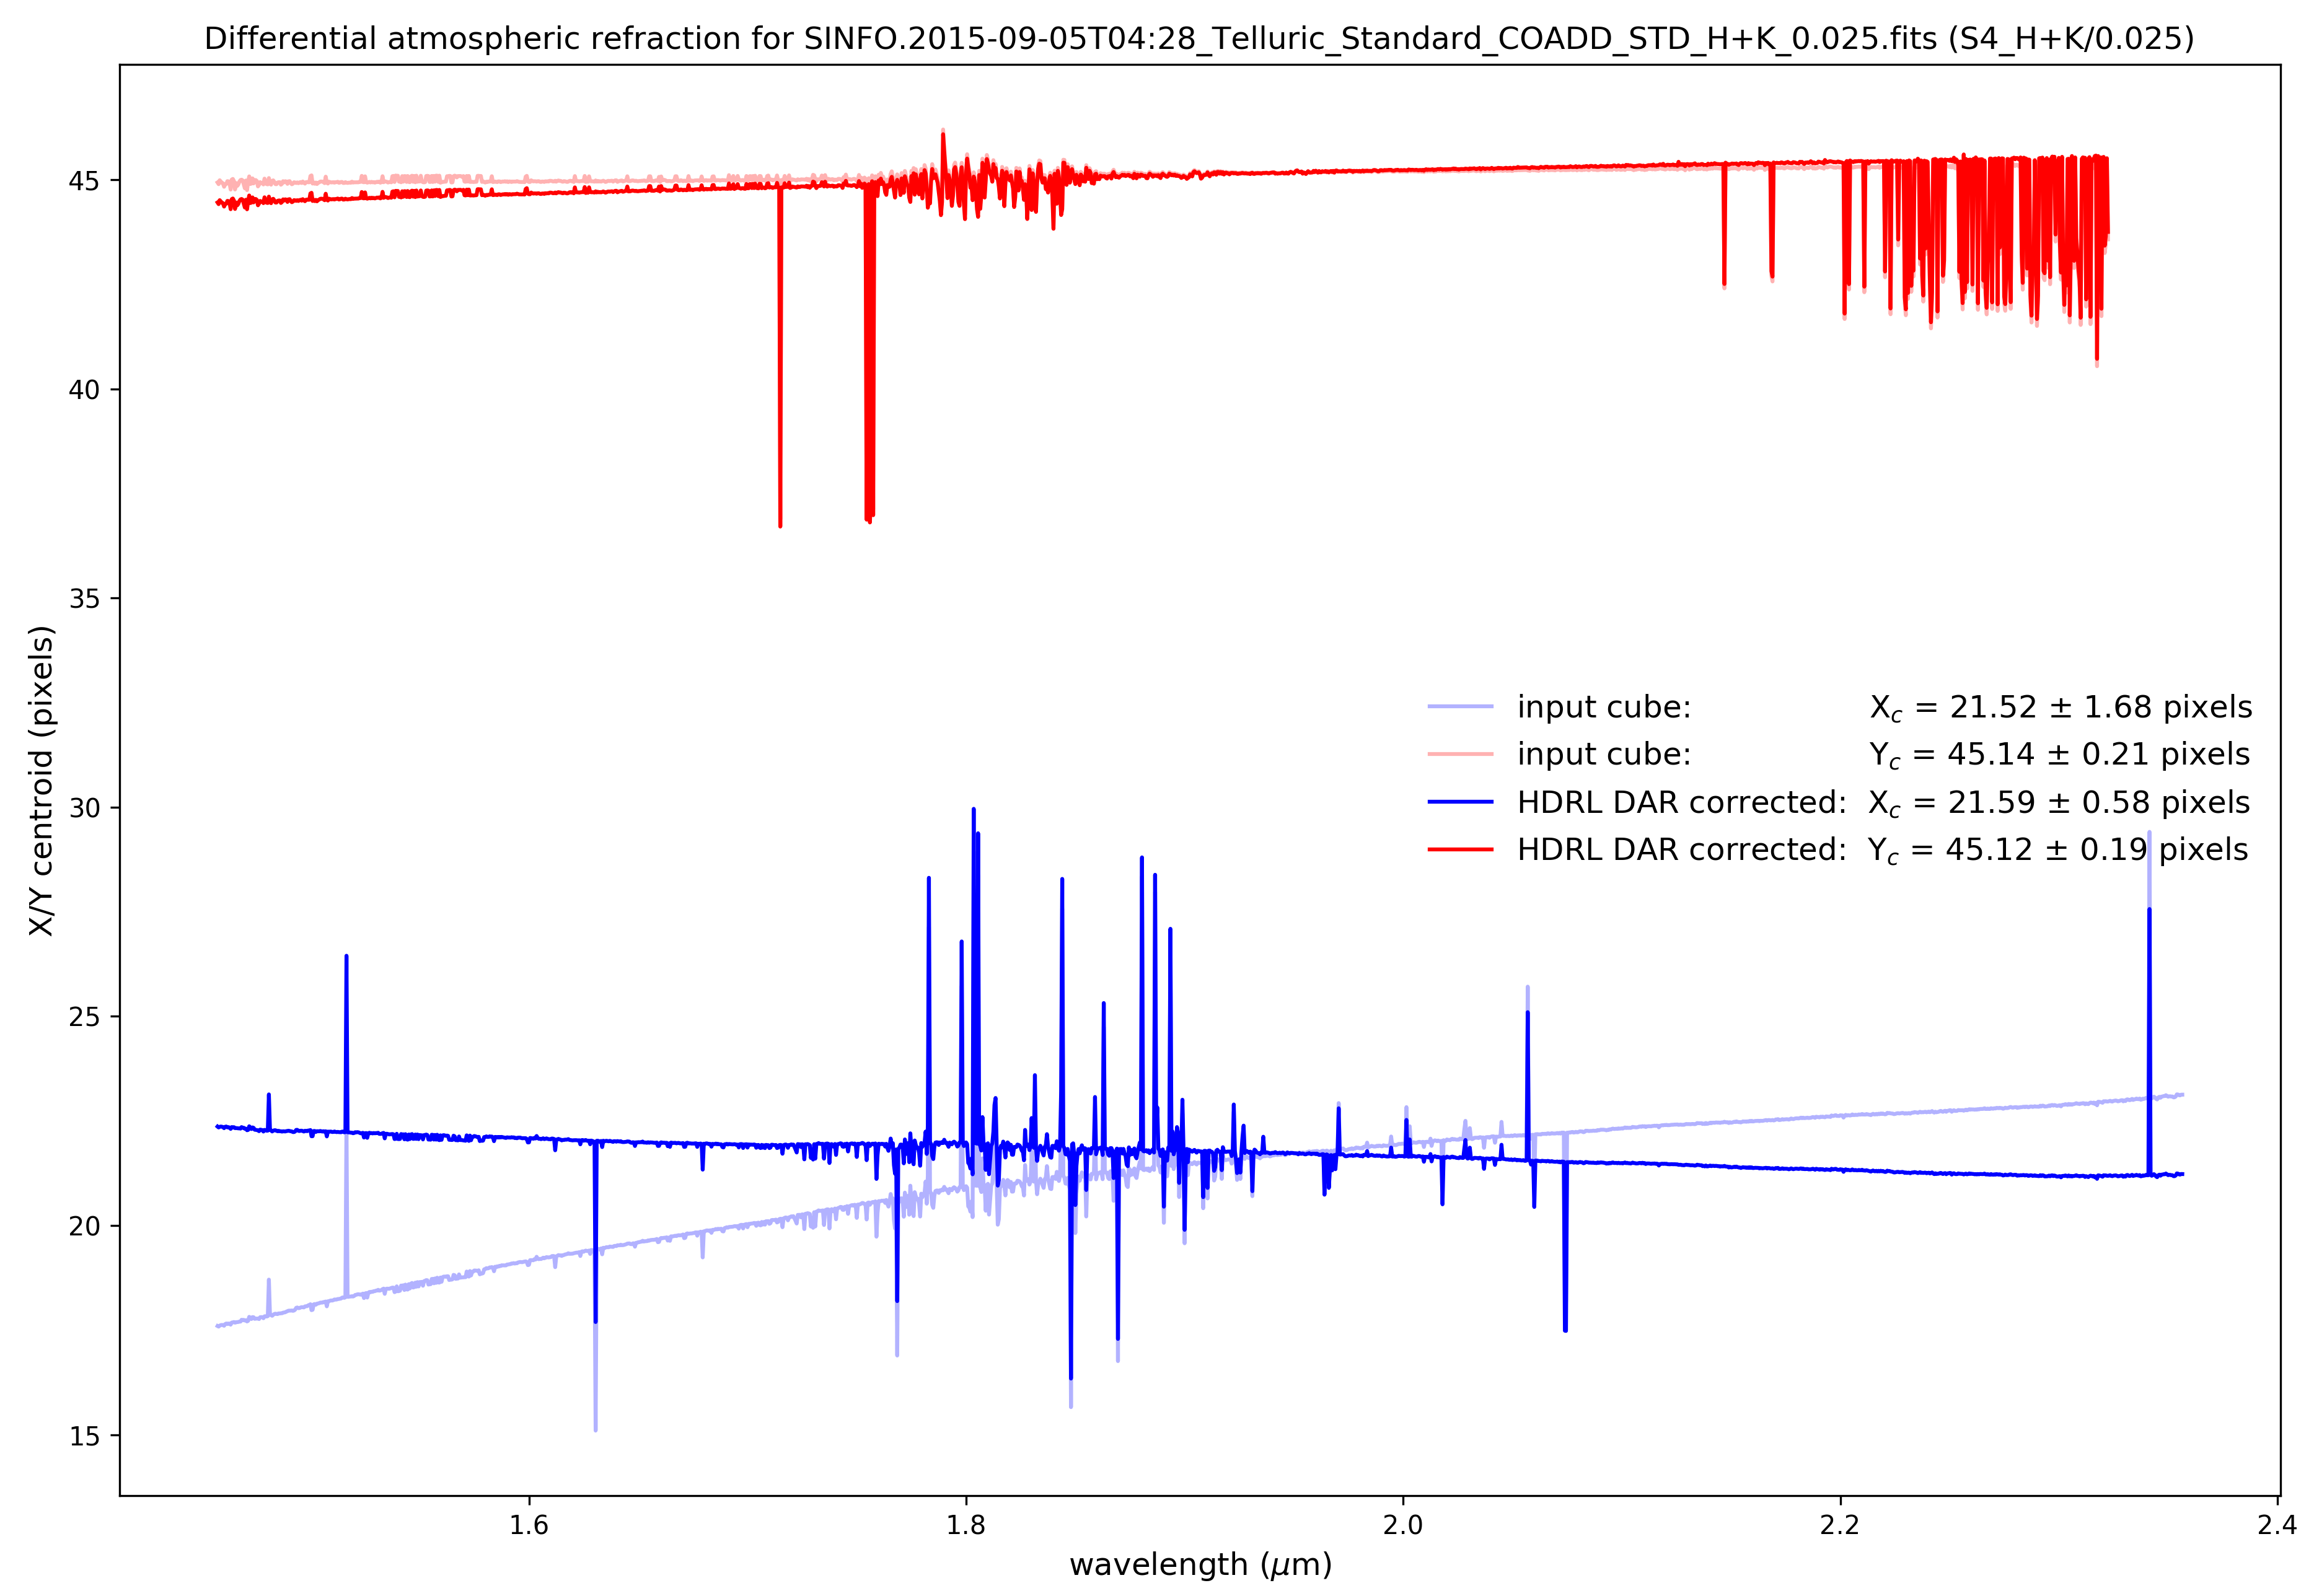
\includegraphics[width=16cm]{figures/SINFO_cube_centroid_corrected.png} 
\caption[]
	{\footnotesize  A line trace of the source centroid position as a function of wavelength for the SINFONI data cube {\tt SINFO.2015-09-05T04:28\_Telluric\_Standard\_COADD\_STD\_H+K\_0.025.fits}.  
	The source centroid is computed through the data cube using the catalogue source-detection module available in \hdrlcat.  
	The blue and red lines are the x-axis  (X$_c$) and y-axis centroids (Y$_c$), respectively.  The faded lines are the raw input data centroids, while the dark lines are the centroids 
	after being corrected for differential atmospheric refraction by \hdrldar.	   The raw data cube has a shift in the source
	centroid, over its full wavelength range, of $\Delta$X$_c$ = 6.9 and $\Delta$Y$_c$ = 0.2 pixels. 
	}
	\label{fig:SINFONI_trace}
\end{figure}

\begin{figure}[H]
\centering \subfigure
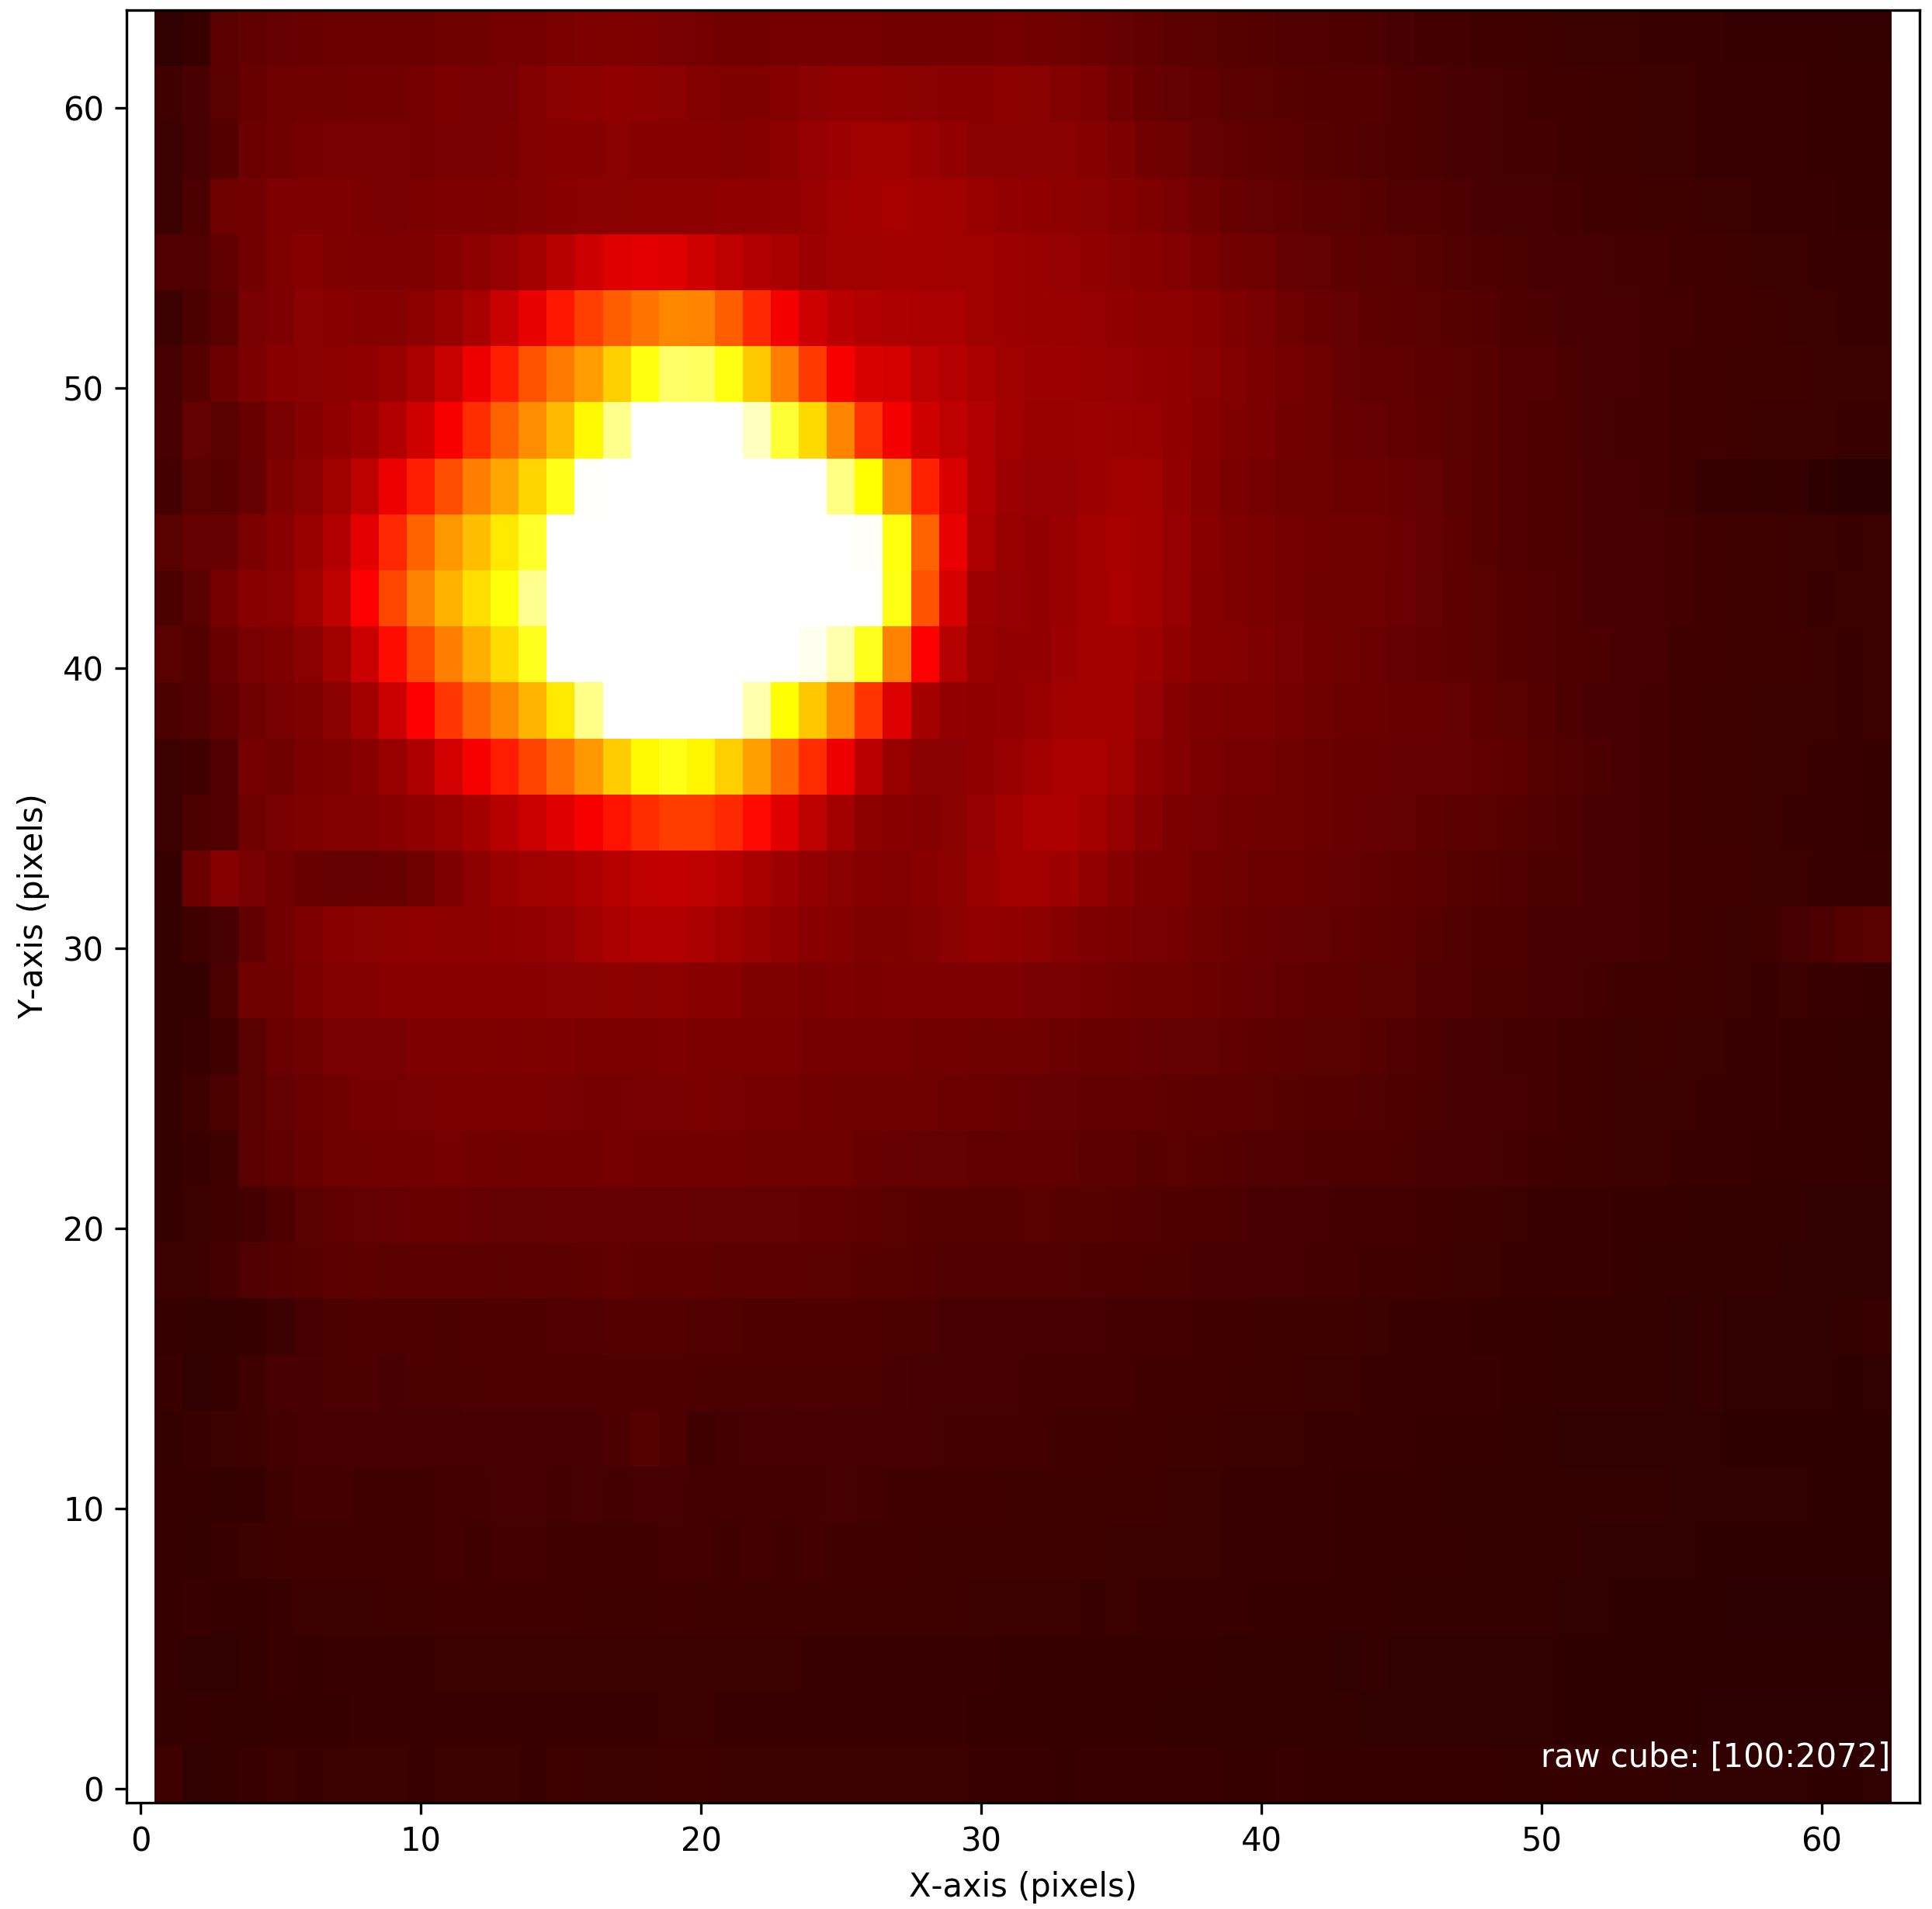
\includegraphics[width=7.8cm]{figures/SINFO_2015-02-18T07:53_Telluric_Standard_COADD_STD_H+K_0_025_full_median_collapsed_cube.png} 
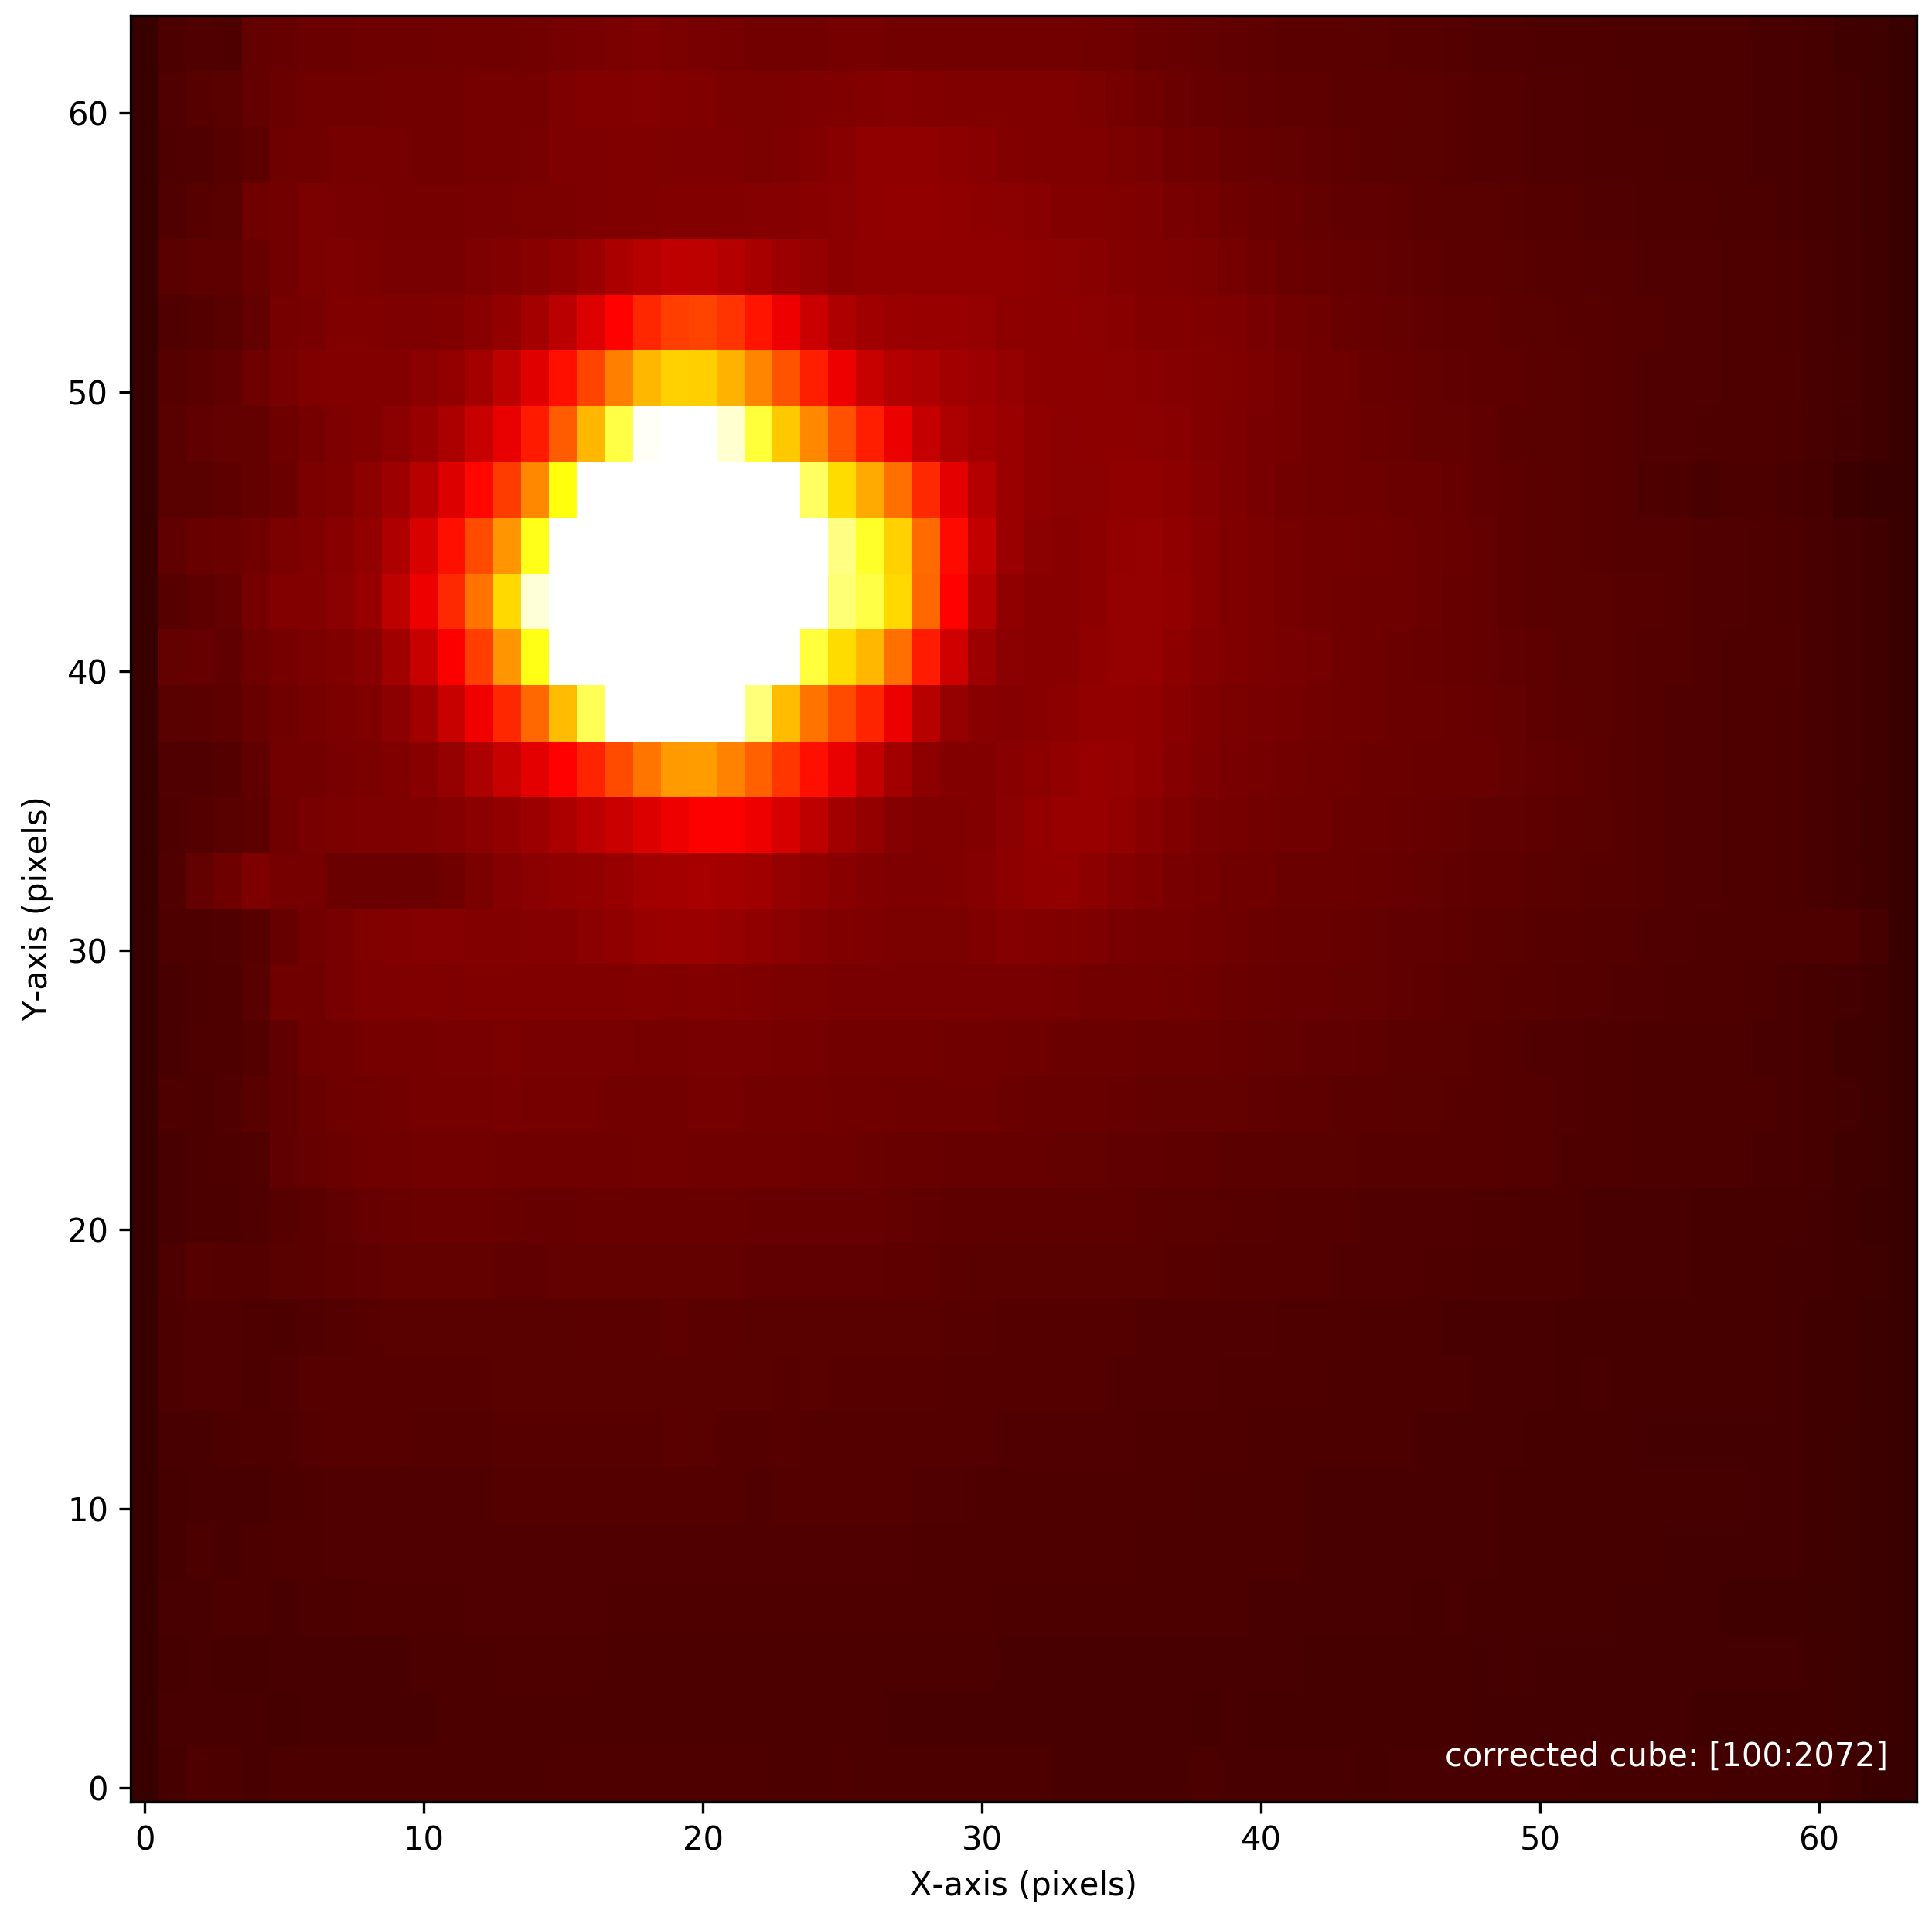
\includegraphics[width=7.8cm]{figures/SINFO_2015-02-18T07:53_Telluric_Standard_COADD_STD_H+K_0_025_full_median_corrected_cube.png} 
\caption[]
	{\footnotesize  {\bf Left Panel:}  A median collapse of the same raw data cube shown as a trace in Figure \ref{fig:SINFONI_trace}. \\
	{\bf Right Panel:}  The same median collapsed cube, integer-pixel-corrected for the differential atmospheric refraction.   The improvement between the raw 
	and corrected data cubes is visually apparent.  A comparison between the raw and corrected frames reveals an x-axis FWHM of
	6.5 and 5.8 pixels, respectively.
	}
	\label{fig:SINFONI_image}
\end{figure}

\subsubsection{II.  Quantitative Results}

In order to quantify the improvements made by applying the theoretical shifts computed by \hdrldar, we define a global atmospheric refraction based the source
position at the end points of each SINFONI data cube (see Figure \ref{fig:global_offsets}).   Using the median value of the source centroid over the first 100 cube planes 
and the last 100 cube planes, we define an overall shift as: 

\begin{align}
\Delta X_c = <X_c> _{100} -  <X_c> _{N_{max} - 100}    \\
\Delta Y_c = <Y_c> _{100} -  <Y_c> _{N_{max} - 100}
\end{align}


\begin{figure}[H]
\centering \subfigure
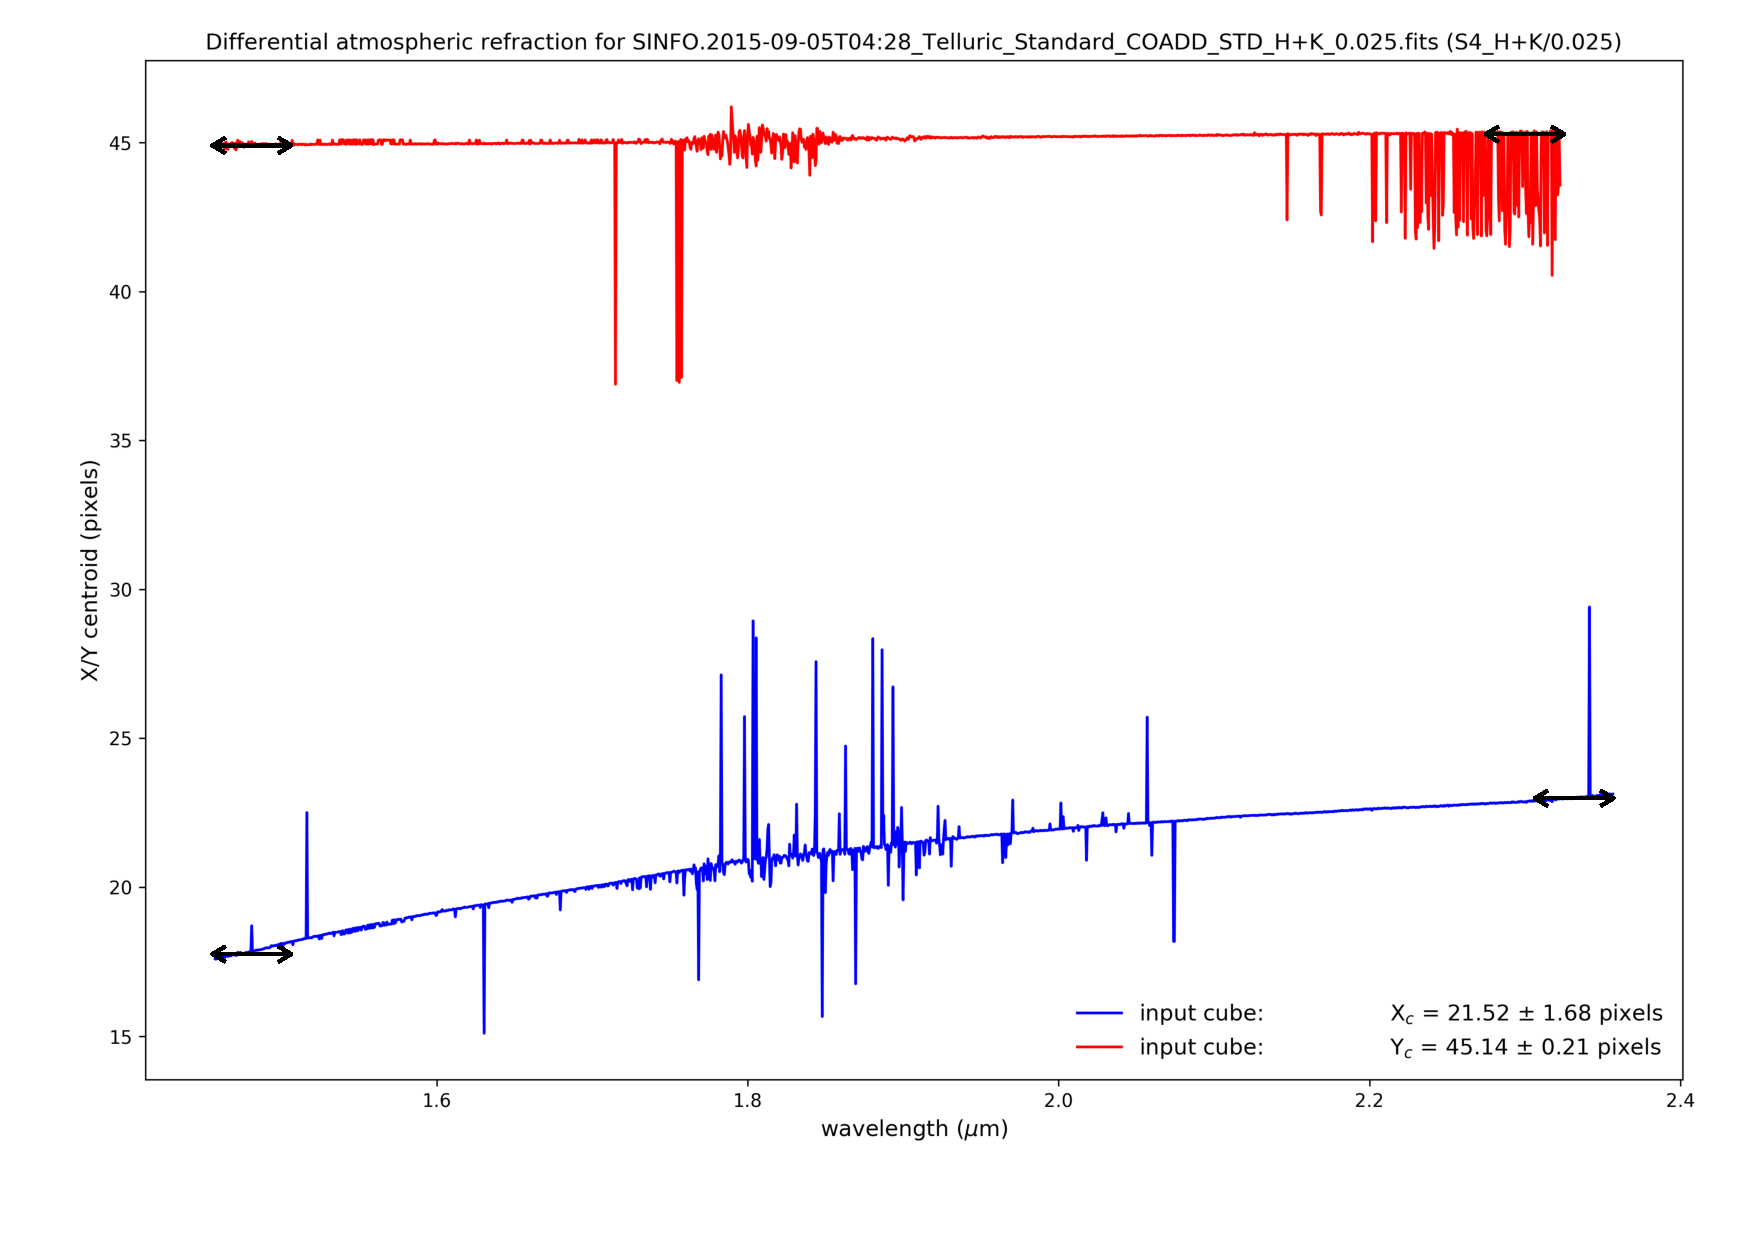
\includegraphics[width=16cm]{figures/define_global_offset.pdf} 
\caption[]
	{\footnotesize  In order to measure the global atmospheric refraction offsets in all SINFONI data cubes, the median centroid position is determined over the first
	100 and the final 100 cube planes.   This is used to define the $\Delta$X$_c$ and $\Delta$Y$_c$.
	}
	\label{fig:global_offsets}
\end{figure}


This global shift is defined for both the measured source centroids and for the theoretically predicted shifts.  For all 754 SINFONI data cubes, we find a very good
match between the measured data offsets and those predicted by \hdrldar:

\begin{align}
\Delta X_c ({\rm data}) -  \Delta X_c ({\rm theory})  = 0.29 \pm 0.63\ {\rm pixels}  \\
\Delta Y_c ({\rm data}) -  \Delta Y_c ({\rm theory})  = 0.02 \pm 0.19\ {\rm pixels}
\end{align}

It should be noted that the reconstructed SINFONI data cubes have rectangular pixels, with the Y-axis pixels being twice as large as those in the X-axis.  This
explains the difference in standard deviation measured in the offsets of equations (3) and (4). 
There appears to be a slight under-correction in the $\Delta X_c$ of about $\frac{1}{3}$ of a pixel.  However, due to the difficulty measuring the source centroids
due to object faintness and/or large background noise, this fraction of a pixel offset is not significant.

The differences between the global offsets measured in the SINFONI data cubes and the offsets predicted by \hdrldar, can be summarised in a surface density
plot displaying $\Delta X_c$(data) - $\Delta X_c$(theory) vs. $\Delta Y_c$(data) - $\Delta Y_c$(theory).   This plot is shown in Figure \ref{fig:surface_density}.


\begin{figure}[H]
\centering \subfigure
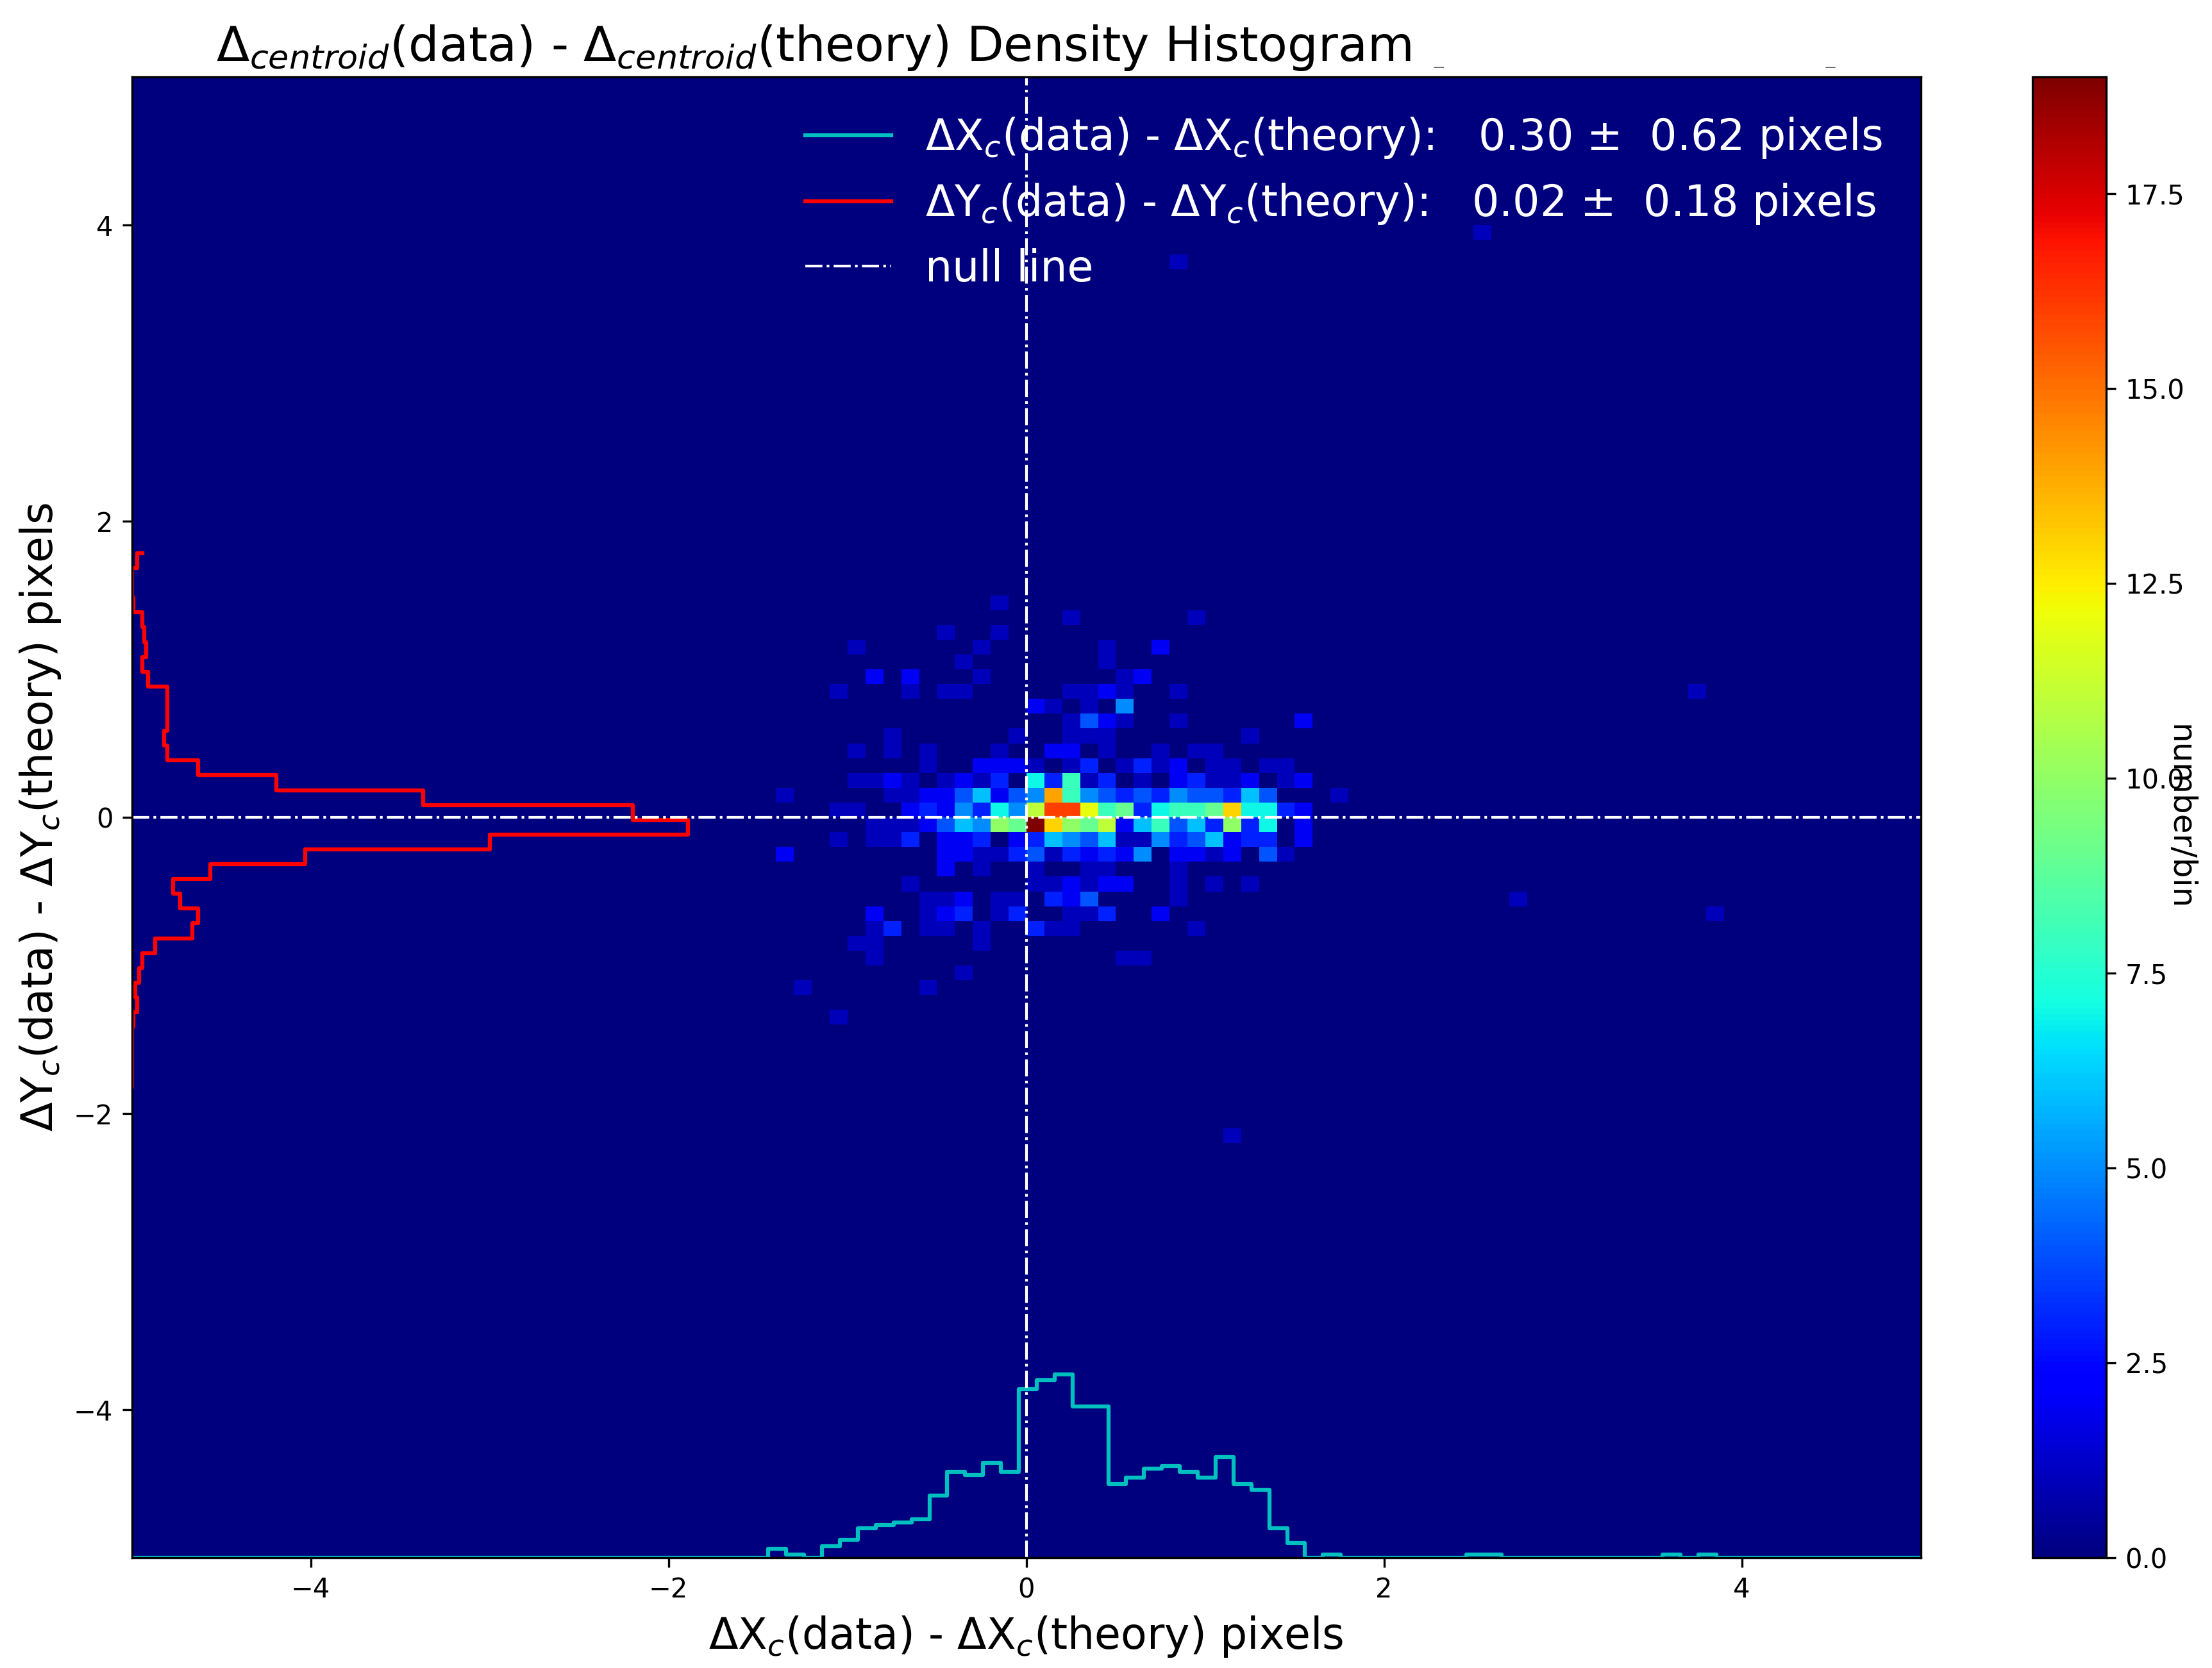
\includegraphics[width=15cm]{figures/SINFO_DAR_2014_2015_2016_surface_density.png} 
\caption[]
	{\footnotesize  Surface density plot of $\Delta X_c$(data) - $\Delta X_c$(theory) vs. $\Delta Y_c$(data) - $\Delta Y_c$(theory) for the 754 SINFONI data
	cubes analysed.  Note that the differing widths of the $\Delta X_c$ and $\Delta Y_c$ histograms is due to the fact that SINFONI has rectangular pixels
	in a 1:2 ratio for $X$:$Y$.
	}
	\label{fig:surface_density}
\end{figure}


An alternative measure of the difference between the measured and predicted offsets can be done using the residuals.  For each SINFONI data cube,
the median centroid position of the standard star was measured ($<X_c>$, $<Y_c>$).  Then, for each cube plane the shift predicted by \hdrldar\ was
added to the measured value of the source centroid and subtracted from the median centroid position.   Thus, the residuals were computed as:

\begin{align}
X_c \, {\rm residual}    =    |  <X_c ({\rm data})>  -  [X_c ({\rm data})  +  X_{\rm shift} ({\rm theory})]\  |  \hspace*{0.5cm} {\rm pixels}  \\
Y_c \, {\rm residual}    =    |  <Y_c ({\rm data})>  -  [X_c ({\rm data})  +  Y_{\rm shift} ({\rm theory})]\  |  \hspace*{0.5cm} {\rm pixels}
\end{align}

A surface density plot of these residuals are shown in Figure \ref{fig:residual_density}.  

\begin{align}
X_c \, {\rm residual}    =    0.15 \pm 0.13  \hspace*{0.5cm} {\rm pixels}  \\
Y_c \, {\rm residual}    =    0.04 \pm 0.03  \hspace*{0.5cm} {\rm pixels}
\end{align}

\begin{figure}[H]
\centering \subfigure
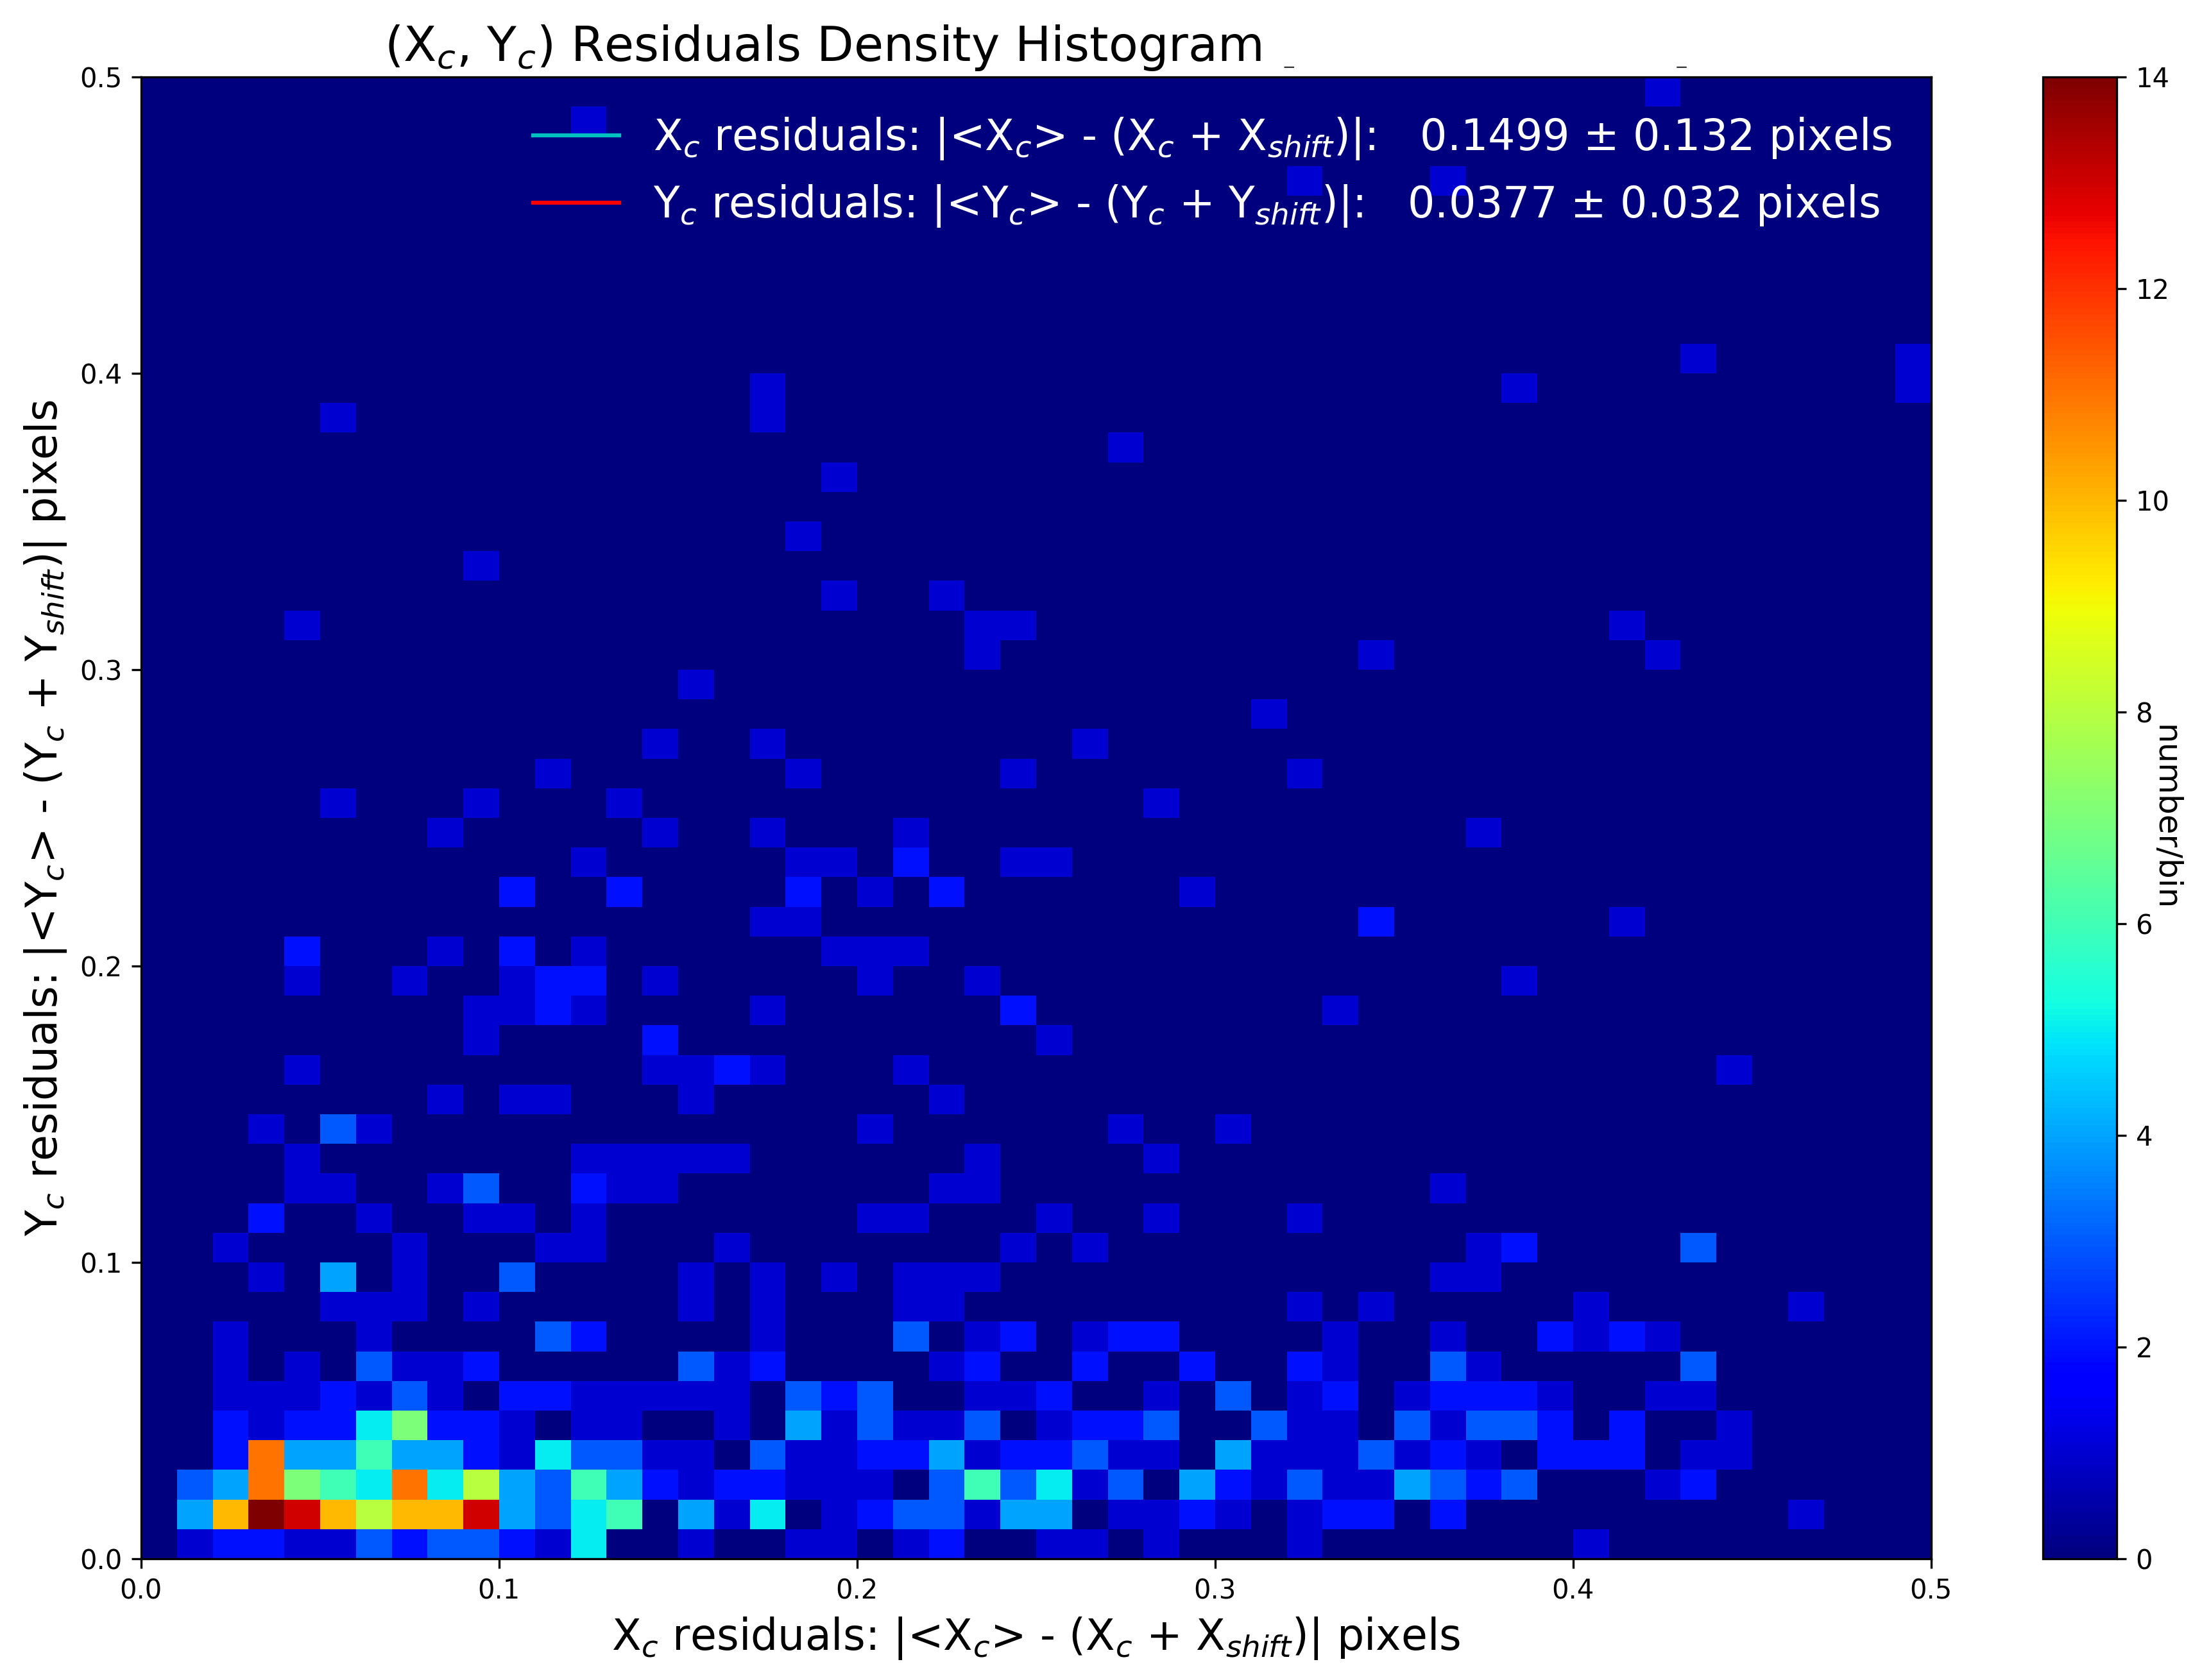
\includegraphics[width=16cm]{figures/SINFO_DAR_2014_2015_2016_residual_density.png} 
\caption[]
	{\footnotesize  Surface density residual plot of $|  <X_c ({\rm data})>  -  [X_c ({\rm data})  +  X_{\rm shift} ({\rm theory})]\  |$ vs. 
	$|  <Y_c ({\rm data})>  -  [X_c ({\rm data})  +  Y_{\rm shift} ({\rm theory})]\  |$ for the 753 SINFONI data
	cubes analysed.  Note that the differing widths of the $\Delta X_c$ and $\Delta Y_c$ histograms is due to the fact that SINFONI has rectangular pixels
	in a 1:2 ratio for $X$:$Y$.
	}
	\label{fig:residual_density}
\end{figure}

\subsubsection{The Strehl Ratios in \hdrldar-Corrected Images}

A further test was made of the improvements possible in the image quality when the \hdrldar\ correction is applied to the SINFONI standard star data cubes.
\hdrldar\ uses its calculated shifts as a function of wavelength, summarised in the results table ({\tt HDRLDEMO\_DAR\_RESULT}), to apply an integer correction 
to the source position.  This is done as the simplest correction and to avoid having to interpolate.

For each corrected data cube a median collapsed image was create and compared to the median collapsed image of the input data cube (an example of this can be
seen in Figure \ref{fig:SINFONI_image}).   For each image, {\tt SExtractor} was run using a detection and analysis threshold of 3$\sigma$.  The \hdrlstrehl\ routine
was then run on the same image using a {\tt flux-radius} set to 1.5$\times$FWHM computed by {\tt SExtractor}.   The {\tt bkg-radius-low} was set to 2.0$\times$FWHM and the
{\tt bkg-radius-high} was set to 3.0$\times$FWHM.  This analysis was restricted to the SINFONI standard star data cubes that show the largest atmospheric refraction; namely,
the $J$ and $H+K$ filters with the 25\,mas pixel scale.   The strehl ratio distributions for the 126 uncorrected (raw) and corrected data cubes are shown as histograms in 
Figure \ref{fig:strehl}.   The corrected data (green histogram) shows a marked improvement over the uncorrected data, with both the strehl median and standard deviation being 
reduced by 26\% and 32\%, respectively.  Since only an integer shift correction was made, this can be considered a lower-limit to the strehl improvement that is possible
when applying \hdrldar\ corrections.


\begin{figure}[H]
\centering \subfigure
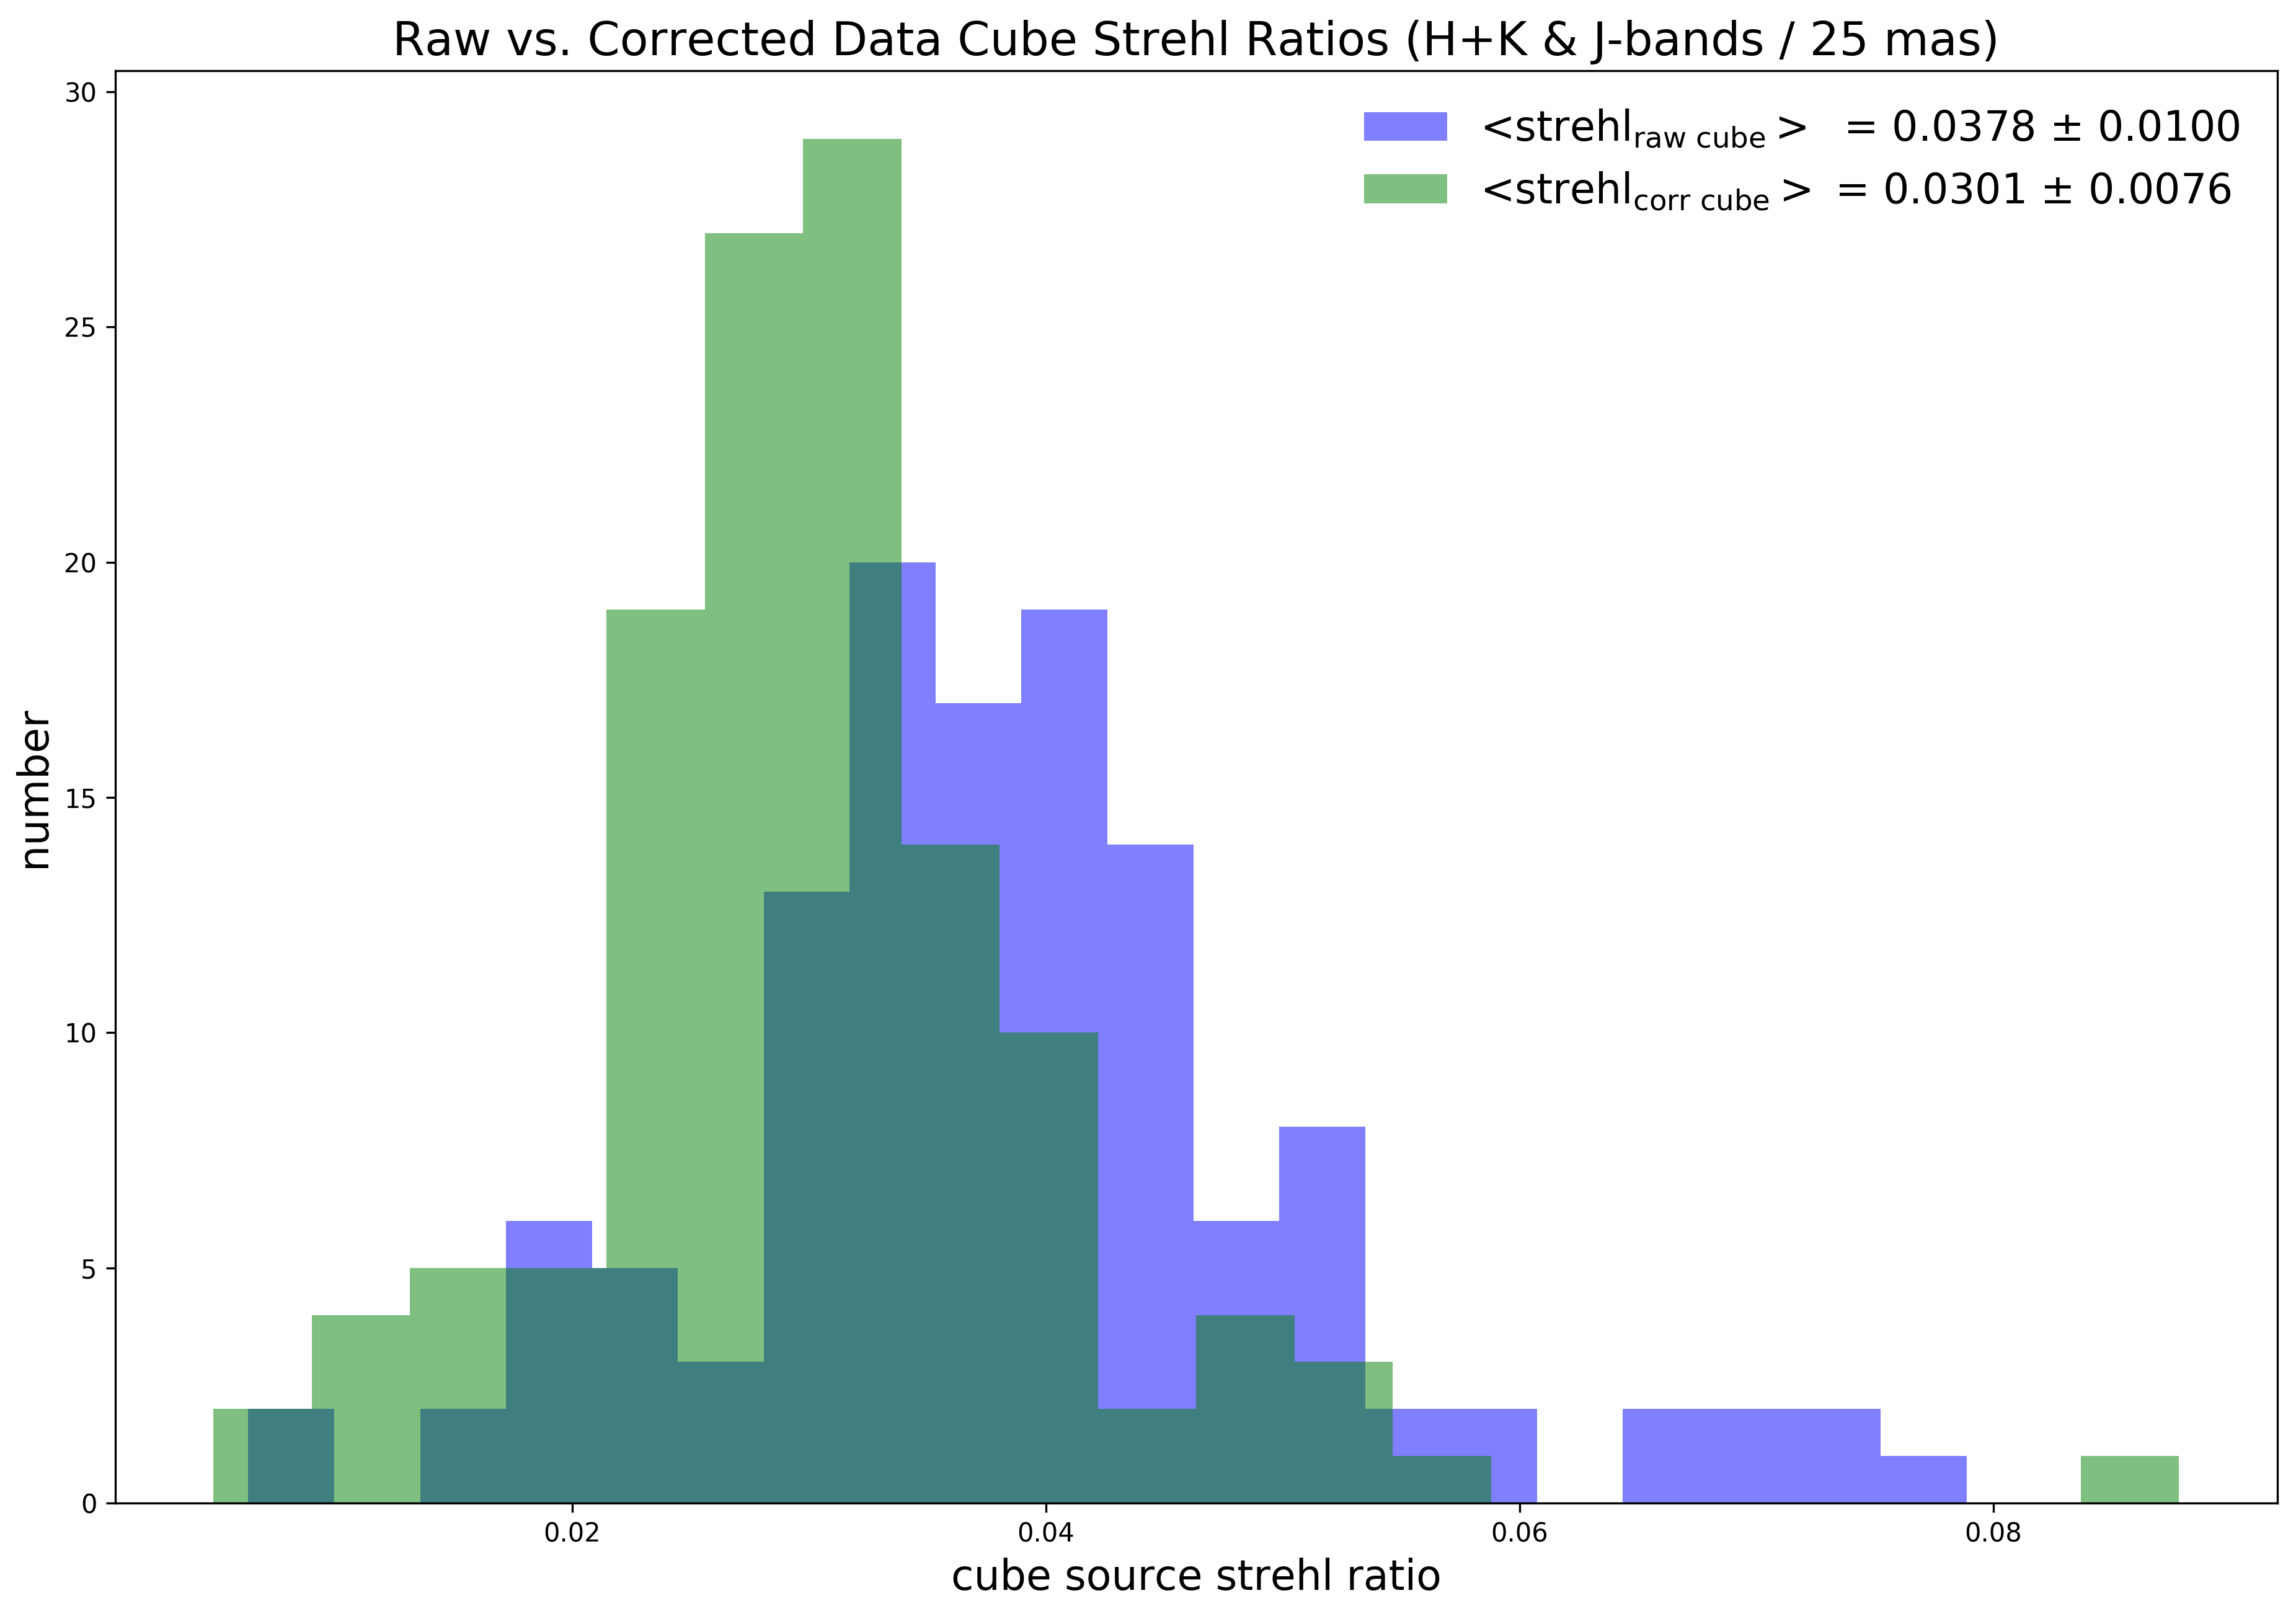
\includegraphics[width=16cm]{figures/SINFO_DAR_2014_2015_2016_HK_J_0_025_strehl20.png} 
\caption[]
	{\footnotesize  A comparison between strehl ratios measured on the median collapsed SINFONI data cubes.  The blue histogram shows the strehl ratios of the original
	data while the green histogram shows the strehl ratios of data corrected for differential atmospheric refraction using \hdrldar.  The data is restricted to the 126 SINFONI
	cubes with 25 mas pixels scale as these have the largest displacements.  The \hdrldar\ correction of the differential atmospheric refraction employed integer pixel shifts only.  
	No interpolation was done.  Despite this, the improvement is significant both in terms of the histogram distribution and in the 26\% improvement in the median strehl ratio.
	}
	\label{fig:strehl}
\end{figure}






\section{Fixed Pattern Noise}
\label{chap:patternnoise}

\def\hdrlfpn{{\em hdrl\_fpn}}

The pattern noise (PN, hereafter) is an almost regular pattern that 
appears on the images. Most likely it is due to electronic 
interference. Perhaps, the simplest PN example is the odd-even 
column/row effect -- a pattern in which consecutive
columns/rows  
have systematically different levels. 
Despite being called {\bf fixed}, the PN is transient and can vary
significantly between frames  of a sequence.

The PN not easily detectable by simple visual image inspection: a 
``good'' image (Fig. \ref{fig:patternnoise_non_diff}, left) is not 
much different from a ``bad'' image (Fig. \ref{fig:patternnoise_non_diff}, 
right), because the amplitude of the pattern may easily be smaller 
than the random noise level. In the special case when the pattern 
is aligned along the columns/rows, compacting the image in the 
direction of alignment can help to make the PN visible, but this 
is not the possible in general.

\begin{figure}[H]
  \centering \subfigure
  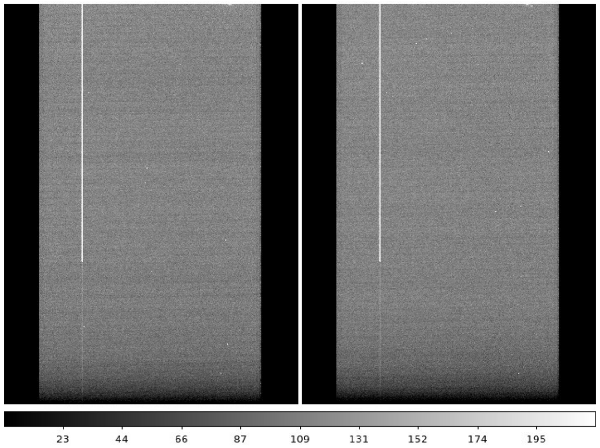
\includegraphics[width=10.0cm]{figures/patternnoise_non-diff.png} 
  \caption[]{\footnotesize Raw GIRAFFE bias images. The vertical stripe 
  is a detector artifact. Here and in the next figures, except for 
  Fig. \ref{fig:patternnoise_test_image}, the left and the right panels 
  use the same stretch to facilitate easier comparison. Here and further 
  the units are ADU.}
  \label{fig:patternnoise_non_diff}
\end{figure}

Fortunately, the PN shows prominently as a set of structures in the power 
spectra. The power spectrum of an ideal image, without any 
pattern, is a perfect delta function with a width of one pixel
(Fig. \ref{fig:patternnoise_test_image}).
The power concentrated in that single peak reflects the simple 
pixel-to-pixel sensitivity variation that is corrected by flat 
fielding. 
Other peaks and structures in the power spectrum indicate the 
presence of systematic noises, e.g. patterns.

However, if the analysed image is a science frame
and contains astronomical objects, these objects themselves will 
introduce peaks in the power spectrum that correspond to variations
on the scales of these objects. Therefore, the search for PN should
be performed on calibration frames, e.g. biases.

The function described here calculates the 2D power spectrum of an
input image, then masks a region around the peak corresponding to
the pixel-to-pixel variations, and then calculates on the remaining 
area of the power spectrum the root mean square (RMS) and the 
mean-absolute-deviation (MAD). A high RMS indicates the presence of
power in variations of any spatial scale and type of PN. The MAD is 
used as a reference level -- it indicates the typical level of the 
random variations of any scale. 

Summarizing, the advantage of this diagnostics is that 
it is sensitive to the PN of any spatial scale or spatial pattern type,
and it is not sensitive to the pixel-to-pixel variations.

\begin{figure}[H]
  \centering \subfigure
  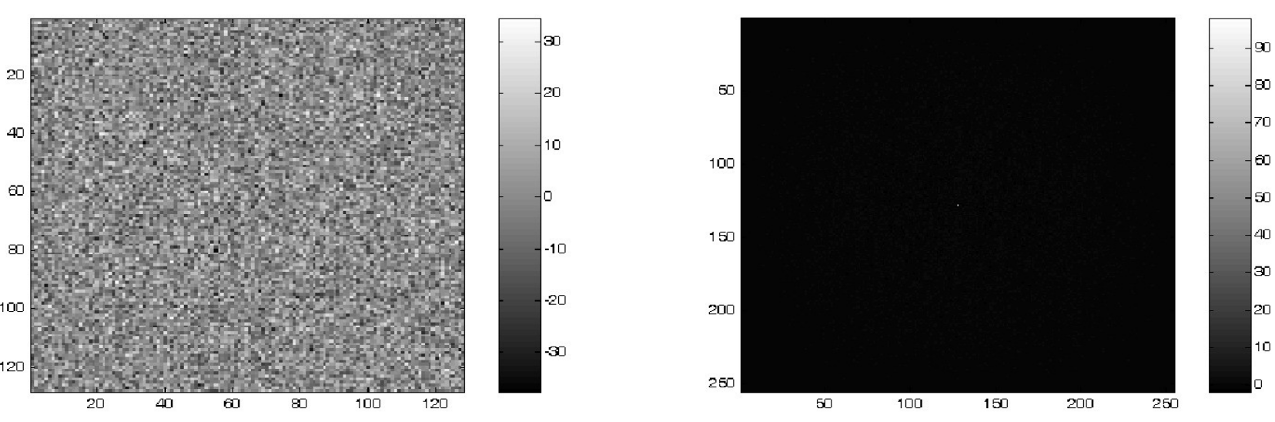
\includegraphics[width=12.0cm]{figures/patternnoise_test-image.png} 
  \caption[]{\footnotesize  {\bf Left Panel:}  Random noise image 
  with no patterns. \\
    {\bf Right Panel:} Its power spectrum (delta function at the centre). }
  \label{fig:patternnoise_test_image}
\end{figure}

Disclaimer: if the described power spectrum 
analysis is applied directly on real raw data, it may be 
affected by any structures such as cosmetic defects (e.g. bad 
columns/areas) and count decrease at the edges (e.g. due to 
vignetting). These changes are systematic in nature and they will 
show prominently in the power spectra, making the signatures 
of the transient PN almost invisible 
(Fig. \ref{fig:patternnoise_giraffe_image}).

\begin{figure}[H]
  \centering \subfigure
  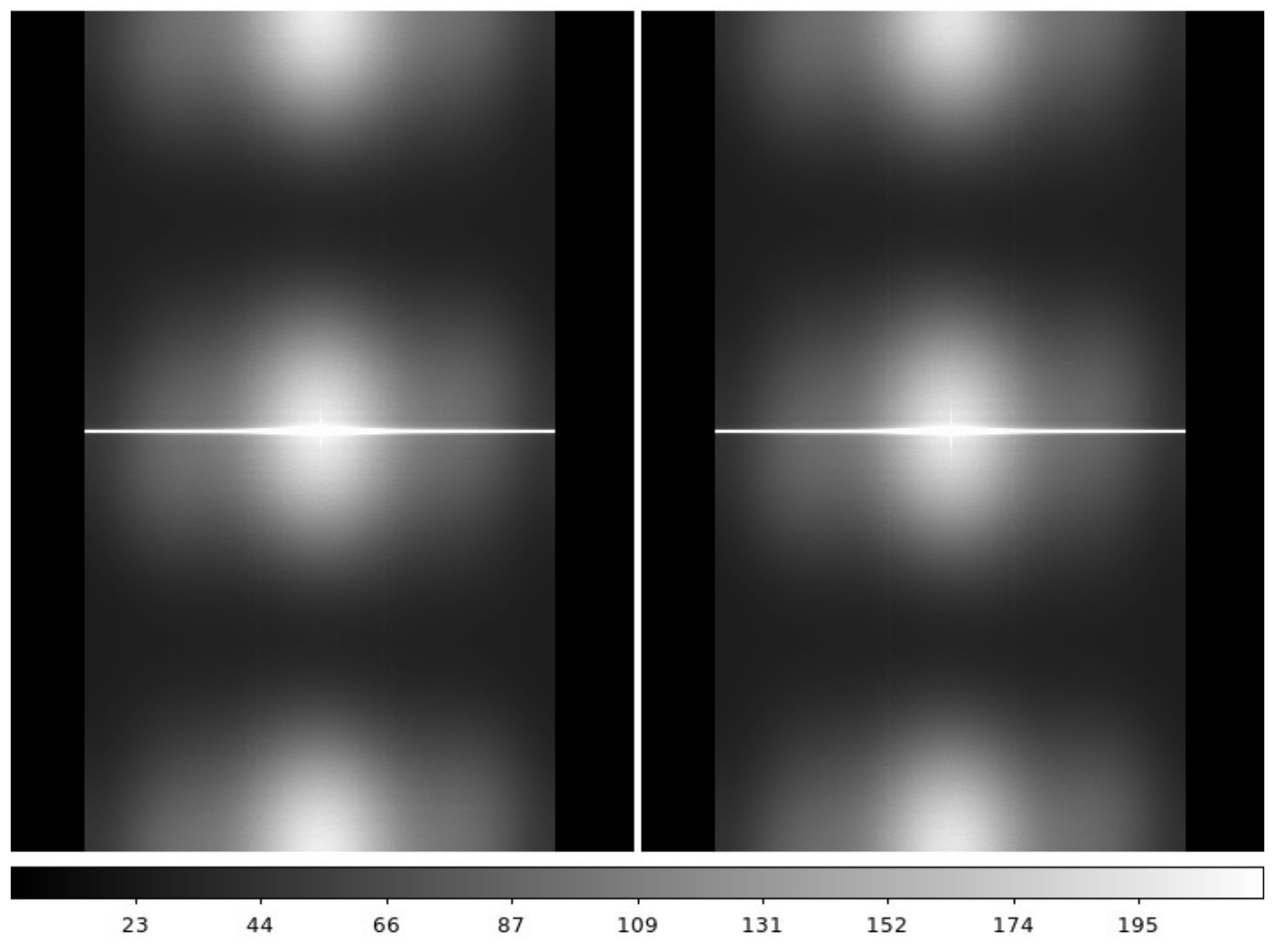
\includegraphics[width=10.0cm]{figures/patternnoise_giraffe-image.png} 
  \caption[]{\footnotesize Power spectra of the raw GIRAFFE bias images.}
  \label{fig:patternnoise_giraffe_image}
\end{figure}

Therefore, some pre-reduction may be necessary: removing the large 
artefacts from the images, repairing the cosmic rays (in our case -- 
replacing the affected pixels with averages from their neighbours), 
and taking out any stable known global patterns like any permanent 
gradients in the illumination or bias level. 
Figure \ref{fig:patternnoise_giraffe_repair_bias} shows an example 
of a ``repaired'' GIRAFFE images).

\begin{figure}[H]
  \centering \subfigure
  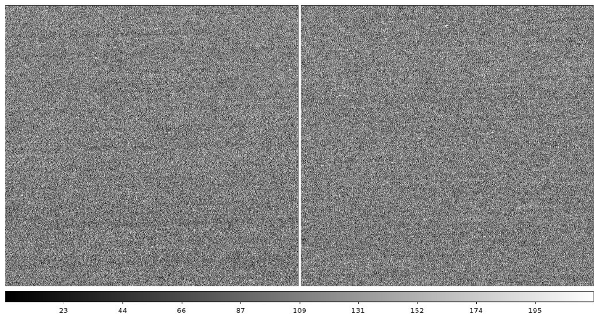
\includegraphics[width=12.0cm]{figures/patternnoise_giraffe-repair_bias.png} 
  \caption[]{\footnotesize ``Repaired'' GIRAFFE bias images.}
  \label{fig:patternnoise_giraffe_repair_bias}
\end{figure}

The power spectra of the ``repaired'' images shows great improvement 
as seen in Fig. \ref{fig:patternnoise_giraffe_repair_powerSpectra} --
compare the weak power present on the left image, and strong power on 
the right image.

The time scale of the PN variations must also be taken into account in this 
analysis, especially if one wants to apply the detection algorithm on 
combined master frames of some kind, e.g. on master biases. If the 
PN varies too quickly, the combination into master bias will average 
over many different types of PN and the resulting image will be 
unrealistically ``clean''. In such cases the analysis should be 
carried out on individual raw images. It is important to investigate 
the PN variation time scale before adopting a procedure for a 
particular instrument/detector.


\begin{figure}[H]
  \centering \subfigure
  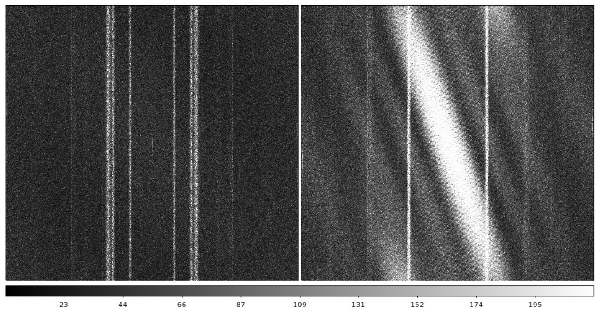
\includegraphics[width=12.0cm]{figures/patternnoise_giraffe-repair_powerSpectra.png} 
  \caption[]{\footnotesize Power spectra of the ``repaired'' GIRAFFE bias. 
  The image on the left shows no pattern noise, the image on the right is 
  affected by pattern noise.}
  \label{fig:patternnoise_giraffe_repair_powerSpectra}
\end{figure}

% To quantify the presence of pattern noise we propose a simple quality 
% control (QC) parameter: fraction of the pixels in the power spectrum that 
% exceed a certain limit. 
% Figure \ref{fig:patternnoise_giraffe_repair_histogram} shows a histogram 
% of this fraction from processing 195 GIRAFFE bias images extracted from 
% the ESO science archive. The adopted limit here was 30 ADU. This limit 
% depends on the instrument detector and the level of removal of any 
% permanent patterns; it must be derived empirically from the data. The 
% images with no pattern noise cluster in the peak centered at a fraction 
% $\sim 0.012 \%$, while the affected images cluster in the peak centered 
% at a fraction $\sim 0.06\%$. A comparison of the top (for not pre-reduced 
% images) and bottom (for reduced images) panels shows that the cleaning of 
% bad columns and pixels improves the separation between the ``good'' and 
% the ``bad'' images. The peak of the affected images is broader, indicating 
% that the pattern noise varies from one image to another.
% 
% 
% \begin{figure}[H]
%   \centering \subfigure
%   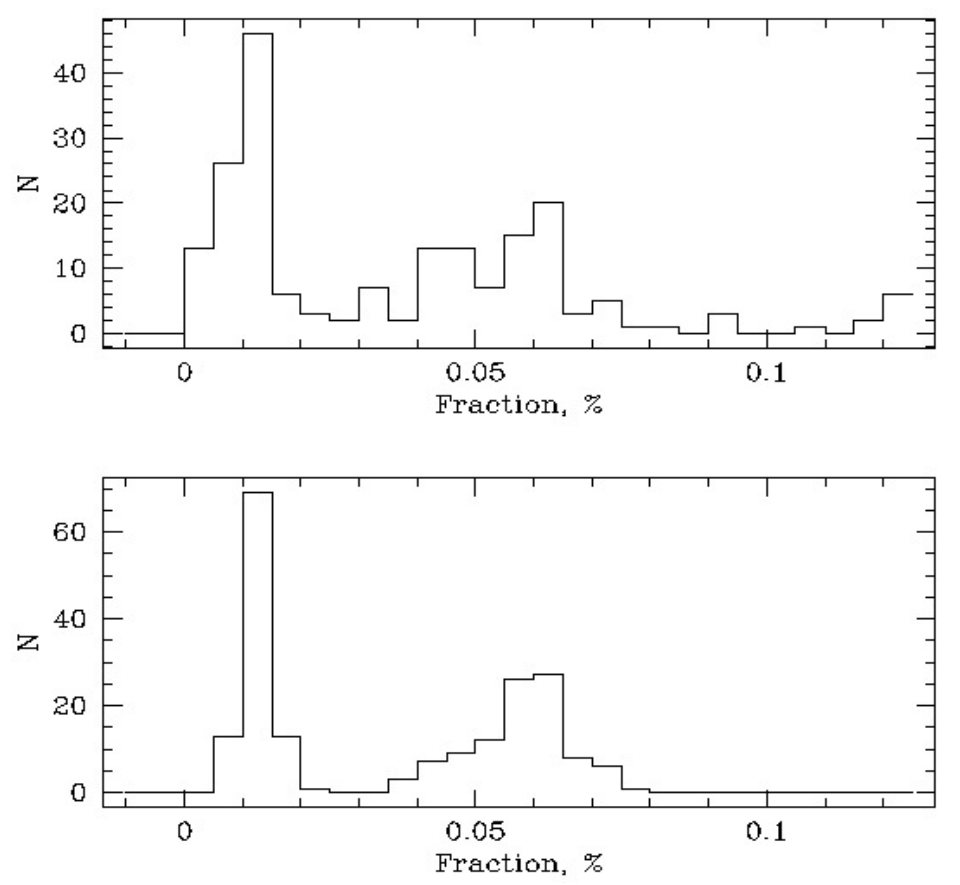
\includegraphics[width=10.0cm]{figures/patternnoise_giraffe-repair_histogram.png} 
%   \caption[]{\footnotesize Histogram of the fraction of pixels (in percent) 
%   above the adopted limit for GIRAFFE raw (top) and ``repaired'' (bottom) 
%   bias images.}
%   \label{fig:patternnoise_giraffe_repair_histogram}
% \end{figure}

% 2020-12-21:    Mark Neeser


\def\sex{{\em SExtractor}}
\def\hdrlresample{{\em hdrldemo\_resample}}
\def\hdrlint{{\em hdrldemo\_interpolation}}



\counterwithin{figure}{section}


\section{Image and Cube Resampling}
\label{chap:assessing:resampling}

\subsection{Introduction}
\label{sect:intro}

The \hdrlint\  implementation consists of a select number of general-use interpolation algorithms for sub-pixel re-gridding in the co-addition of 2D images 
(to be used in a stacking recipe added to the ESOTK package) and in the reconstruction of 3D data cubes. 
The recipes can take images or cubes as input, interpolate them to a common grid and, for the 2D images, co-add the re-gridded images using 
stacking functions already available in HDRL.

General interpolation methods can be relevant to any ESO instrument, however, the core application for the interpolation routines will be the combination 
of multiple, dithered frames to a sub-pixel, re-gridded reference frame. This has applications for both 2D image combination (FORS2) 
and for 3D data cube reconstruction with the integral field spectrographs, HARMONI, ERIS/SPIFFIER, MUSE, and KMOS.

The interpolation palette of \hdrlresample\ consists of the resampling methods {\tt  NEAREST, LINEAR, QUADRATIC, RENKA, LANCZOS,}
and {\tt DRIZZLE}.   The specific attributes of these interpolation algorithms were specified in the original proposal (\cite{Neeser2019}) and include the following:
\begin{itemize}
\item[1.] retain good image quality following the interpolation. For example, their use in a pipeline should not increase the FWHM of a 
Nyquist-sampled Gaussian by more than 20\% (see, for example, \cite{harmoni});
\item[2.] conserve the detected flux over the sampled scale;
\item[3.] allow an estimate of the interpolation error, which is used to compute the variance;
\item[4.] retain the correct pixel status (i.e. propagate bad pixels or exclude them by performing a sigma clipping or another rejection method);
\item[5.] can be, when possible, multi-threaded in order to keep the computation times reasonable;
\end{itemize}

The goal of this report is to verify the use of the six interpolation methods on various types of data (synthetic images, HAWK-I images, strongly rotated images, 
and 3D data cubes), and to test whether all specific goals have been achieved.



\subsection{Testing the \hdrlresample\ Routines Using Synthetic Data}


To test the \hdrlresample\ routines a series of synthetic exposures were created and interpolated.
This data includes both single images and a series of 10 dithered exposures.  

The synthetic images are made using a dedicated Python routine ({\it synthetic\_images.py}) that uses IRAF
the functions {\it iraf.mknoise} to create the image background, {\it iraf.starlist} to create a list of stars with given distributions
and brightness limits,  and {\it iraf.mkobject} to convert this list to images with a {\it Moffat} profile, a given exposure time,
and a given magnitude zero point.  In order to test the changes
that the interpolation introduces to the images, only stellar sources were added to the synthetic images.  The format of the
synthetic images is a three-plane MEF consisting of the image data, the image error, and the quality map.
A summary of the attributes of the synthetic images include:
\begin{itemize}[leftmargin=3cm]
\itemsep0em
\item[size:] 1024$\times$2048 pixels
\item[background:] 500 ADU
\item[gain:] 2.5 e$^{-}$/ADU
\item[readnoise:] 5.0 e$^{-}$
\item[N$_{\rm sources}$:] 1000
\item[exposure time:] 100 sec.
\item[mag zeropoint:] 14.0
\item[N$_{\rm dithers}$:] 10
\item[dither\_step:] 30 pixels
\end{itemize}

These single and 10 dithered images were then resampled using each of the methods available in \hdrlresample, 
{\tt NEAREST, LINEAR, QUADRATIC, RENKA, LANCZOS, and DRIZZLE}, and each was executed with both a 
loop distance of 1 and 3 pixels ({\tt --method.loop-distance}).
The sources within the interpolated images are then compared to the sources in the original input images.

An example of two representative \hdrlresample\ products are shown in figure \ref{fig:synthetic_image}.

\begin{figure}[H]
\centering
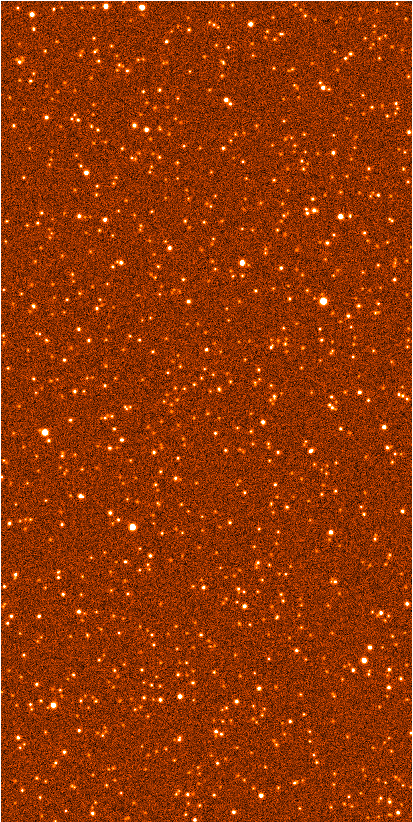
\includegraphics[width=5cm]{figures/synthetic_stars_gal_bkgd_1.png} 
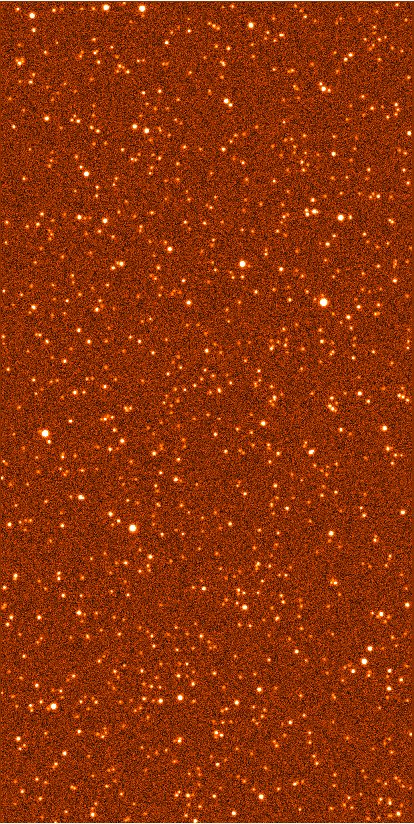
\includegraphics[width=5cm]{figures/hdrldemo_resample_DRIZZLE_single_3.png} 
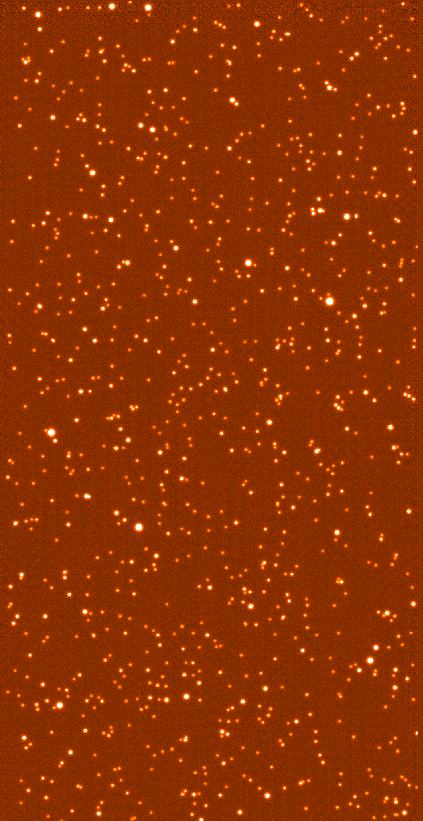
\includegraphics[width=5.115cm]{figures/hdrldemo_resample_DRIZZLE_coadd_3.png} 
\caption[]
	{\footnotesize  {\bf Left Panel:}  An input synthetic image with 1000 stellar sources.\\
	{\bf Centre Panel:}  The resampled single synthetic frame using \hdrlresample\ with {\tt --method=DRIZZLE} and {\tt --method.loop-distance=3}.\\
	{\bf Right Panel:}  The resampled tile of 10 synthetic frame using \hdrlresample\ with {\tt --method=DRIZZLE} and {\tt --method.loop-distance=3}.
	}
	\label{fig:synthetic_image}
\end{figure}


The comparison of the data products is done using a python script ({\tt compare\_image\_sex.py}).  This script runs SExtractor (\cite{bertin})
on both images with a {\tt -DETECT\_THRESH} and {\tt -ANALYSIS\_THRESH} of 5.0\,$\sigma$ and a {\tt -DETECT\_MINAREA} of 10 pixels.
A spherical, nearest-neighbour match within 1 arcsec is then done between the sources of the two resultant SExtractor catalogues.
This allows us to compare the attributes (position ($\alpha, \delta$), magnitude, FWHM, and ellipticity) of the ensemble of extracted sources
from the input synthetic images to the same sources once they have been resampled by each of the six interpolation methods.

In all five methods of image resampling, the astrometric quality of the sources is retained following interpolation.  An example of this is shown in 
Figure \ref{fig:radec_synthetic}.  Here, the absolute positions of the sources in the 10 synthetic images are compared to the absolute positions
of the sources in the image resample using the lanczos method.   Here, the median $\Delta\alpha*\cos(\delta)=0.007\pm0.03\ arcsec$ and 
$\Delta\delta=-0.001\pm0.04\ arcsec$ with the cloud of offsets spread symmetrically about the origin.  
Considering that the synthetic image pixel size is 0.20 pixels/arcsec, the astrometric accuracy is retained to better than a $\frac{1}{5}$ of one pixel (0.04 pixels).

\begin{figure}[H]
\centering
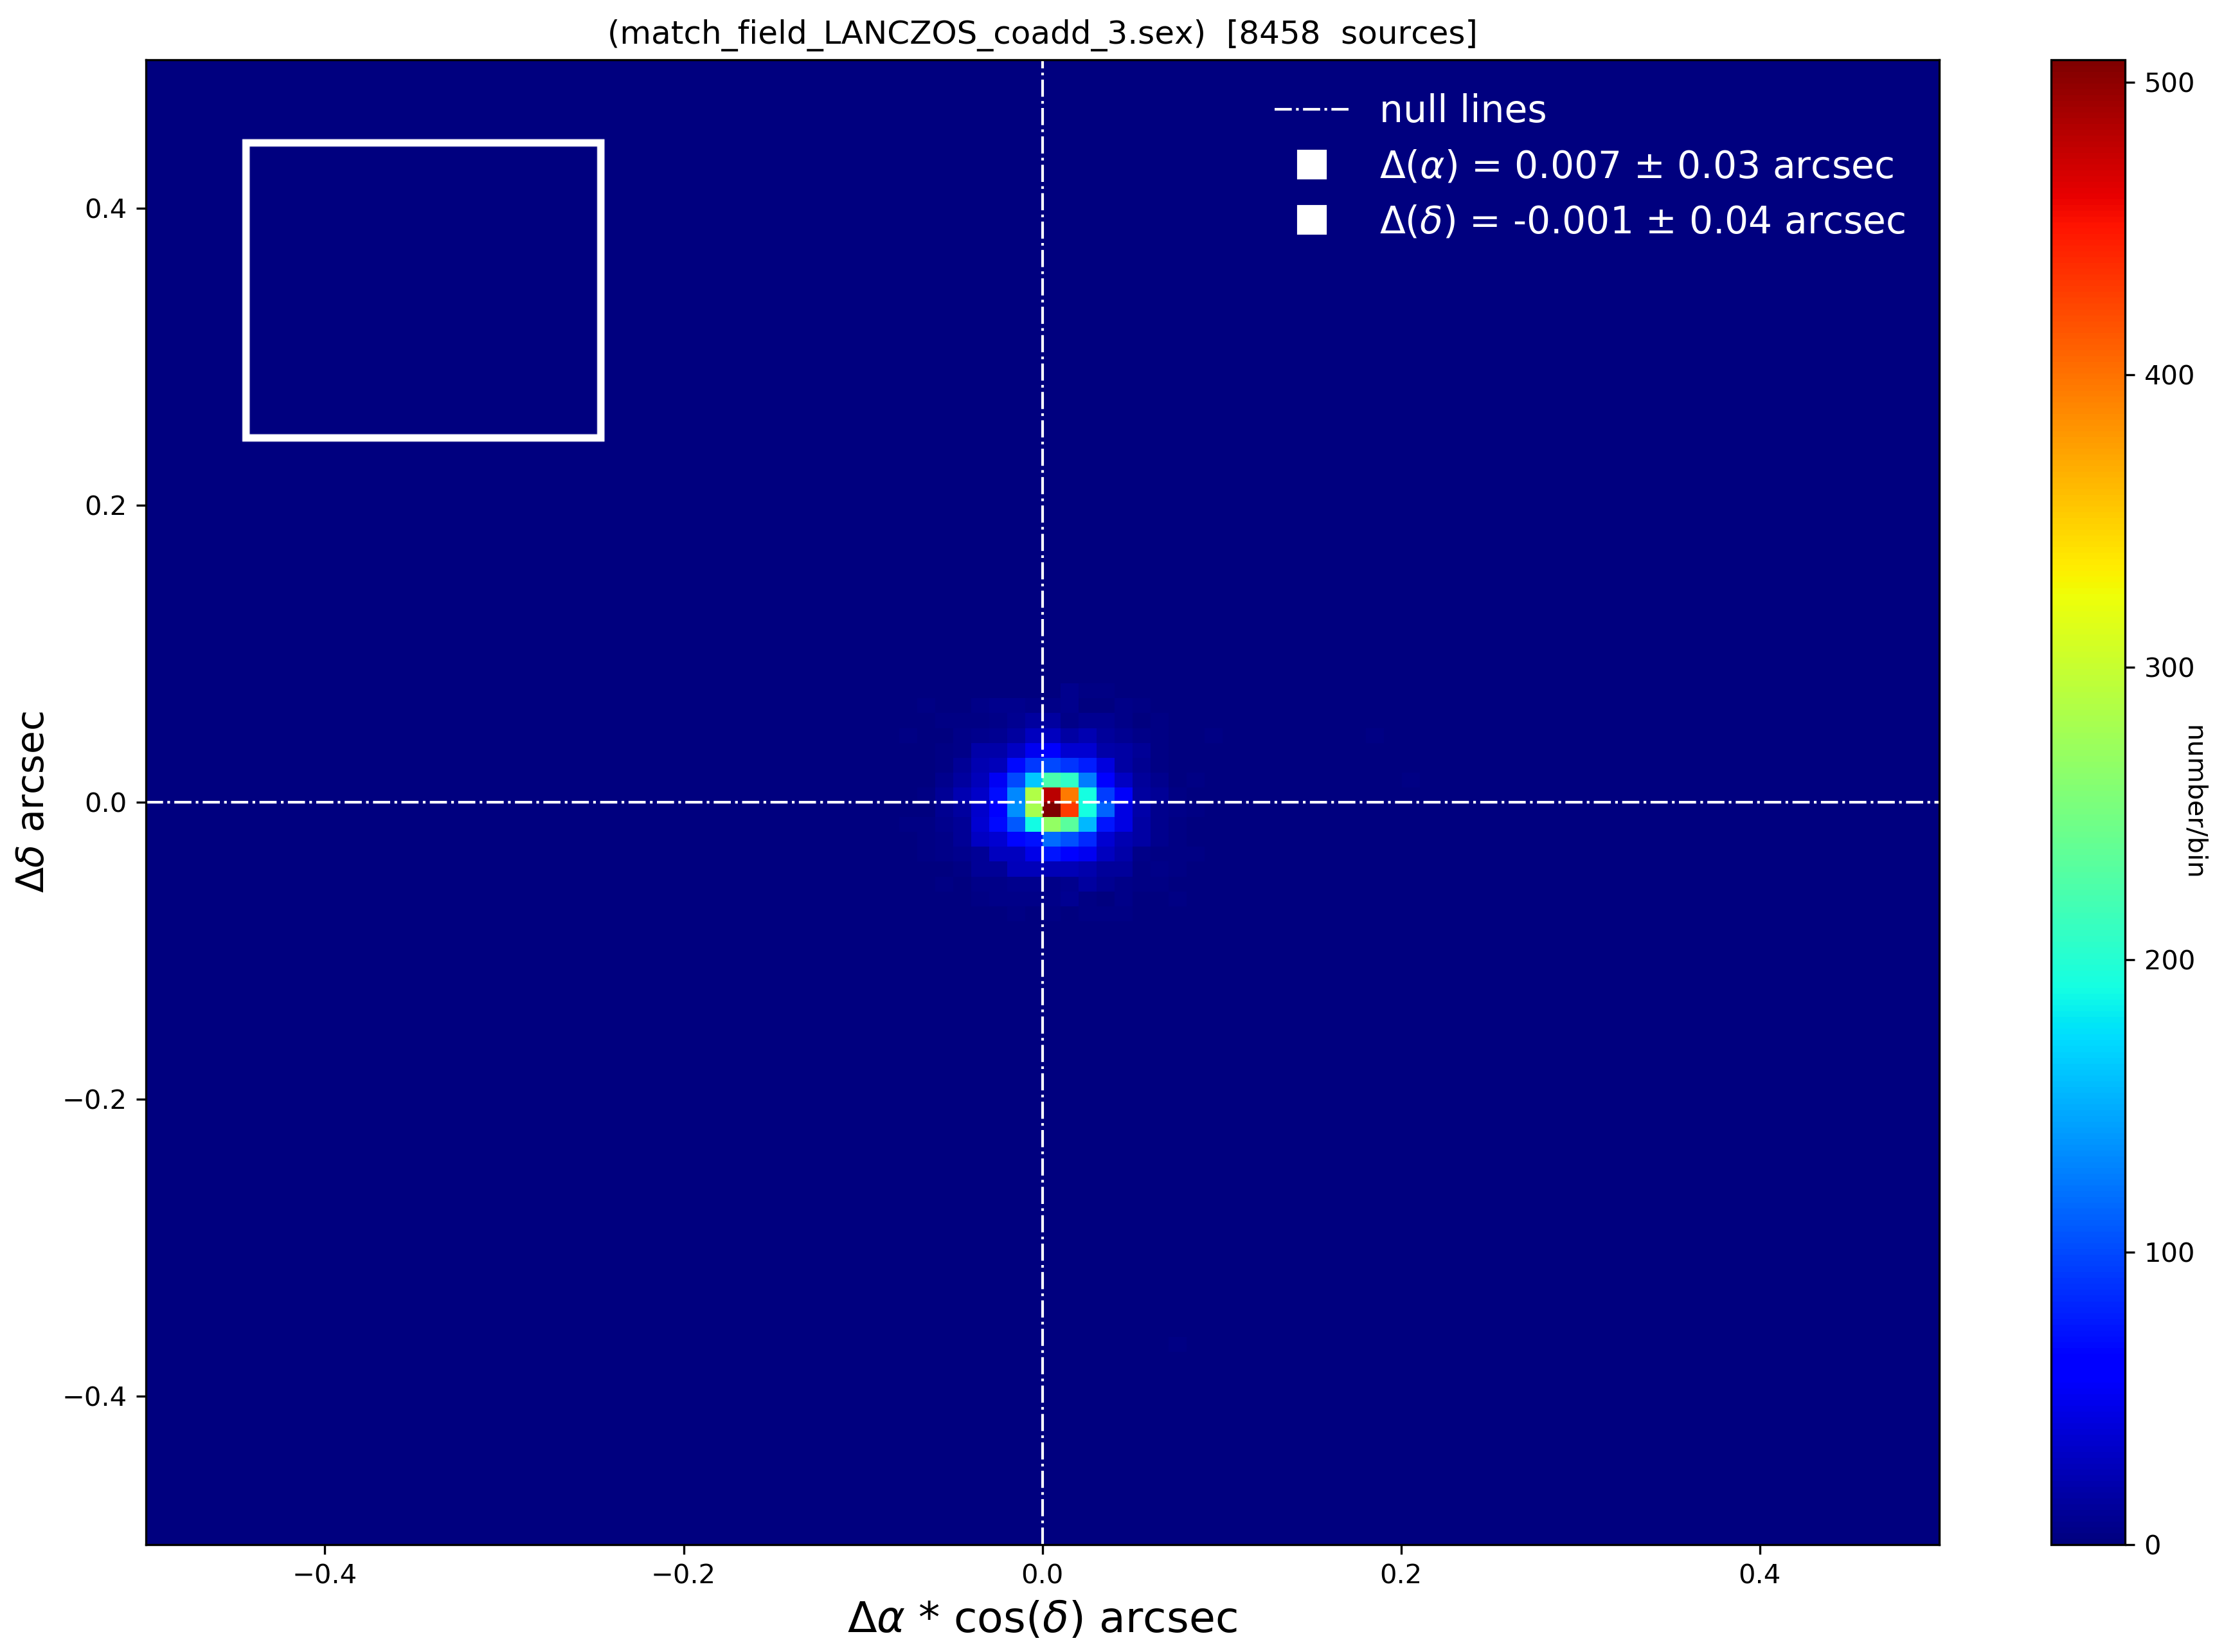
\includegraphics[width=11cm]{figures/match_field_LANCZOS_coadd_3_RA_DEC_scatter_plot.png}
\caption[]
	{\footnotesize  the astrometric quality of the \hdrlresample\ routines as measured by comparing the more than 8,000 sources in the synthetic input images,
	with those in the resampled ({\tt LANCZOS}) image tile.
	The standard deviation of the $\Delta\alpha*\cos(\delta)$ and $\Delta\delta$ distributions is 0.04 arcsec. This is significantly less than one
	pixel (0.20 pixels/arcsec).  The pixel size is indicated by the white square in the top left corner.
	}
	\label{fig:radec_synthetic}
\end{figure}

Similarly, the photometric quality is also retained following interpolation.   Figure \ref{fig:mag_synthetic} is typical of the synthetic interpolated frames, with a source magnitude match 
between the individual images and the resampled (lanczos) image tile of $\Delta(mag)=0.006\pm0.05$ magnitudes.

\begin{figure}[H]
\centering
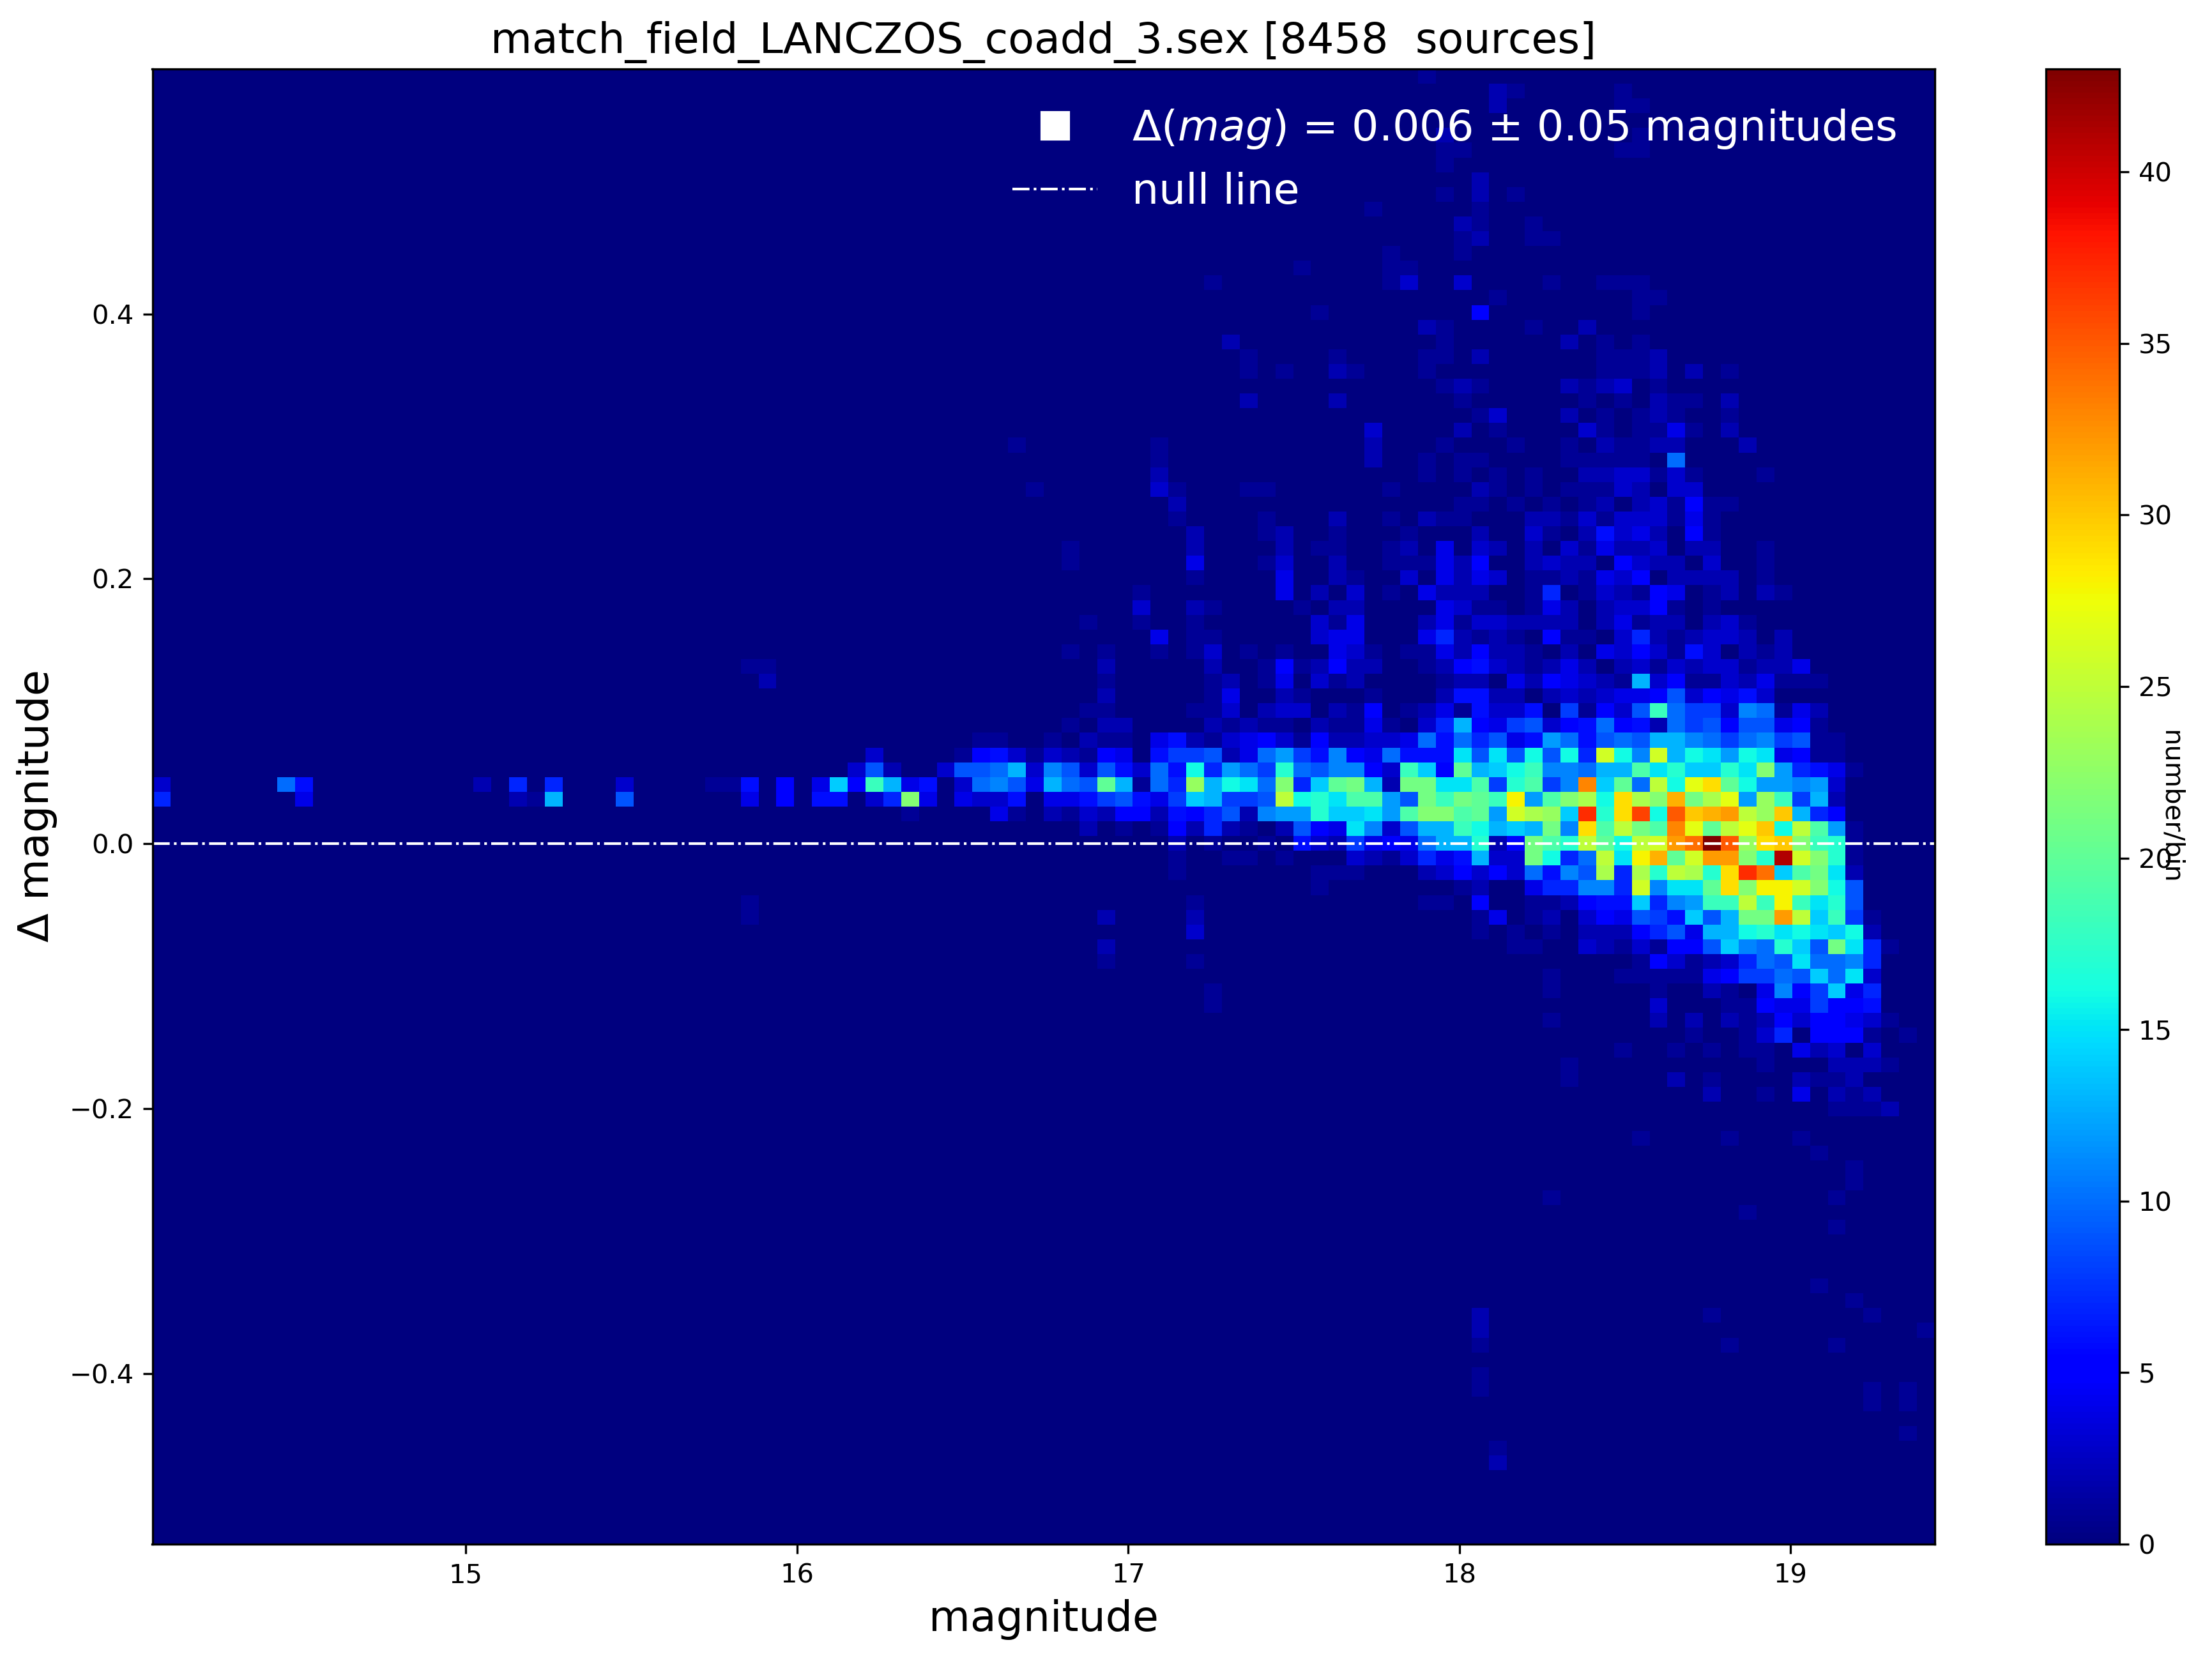
\includegraphics[width=11cm]{figures/match_field_LANCZOS_coadd_3_mag_scatter_plot.png}
\caption[]
	{\footnotesize  the photometric quality of the \hdrlresample\ routines as measured by comparing the more than 8,000 sources in the original input synthetic images
	with those in the resampled (lanczos) image tile.
	The standard deviation of the $\Delta(mag)$  distribution is 0.05 magnitudes. 	
	}
	\label{fig:mag_synthetic}
\end{figure}

As can be seen in figure \ref{fig:fwhm_ellip_synthetic}, the resampling (in this case using {\tt --method=LINEAR}) causes a slight increase in the FWHM of the sources.
This is expected for any interpolation method.   As can be seen in the left panel of Figure \ref{fig:fwhm_ellip_synthetic}, the resampling tightens the distribution of FWHM and
slightly increases it.   This is true for all resampling methods tested.   


\begin{figure}[H]
\centering
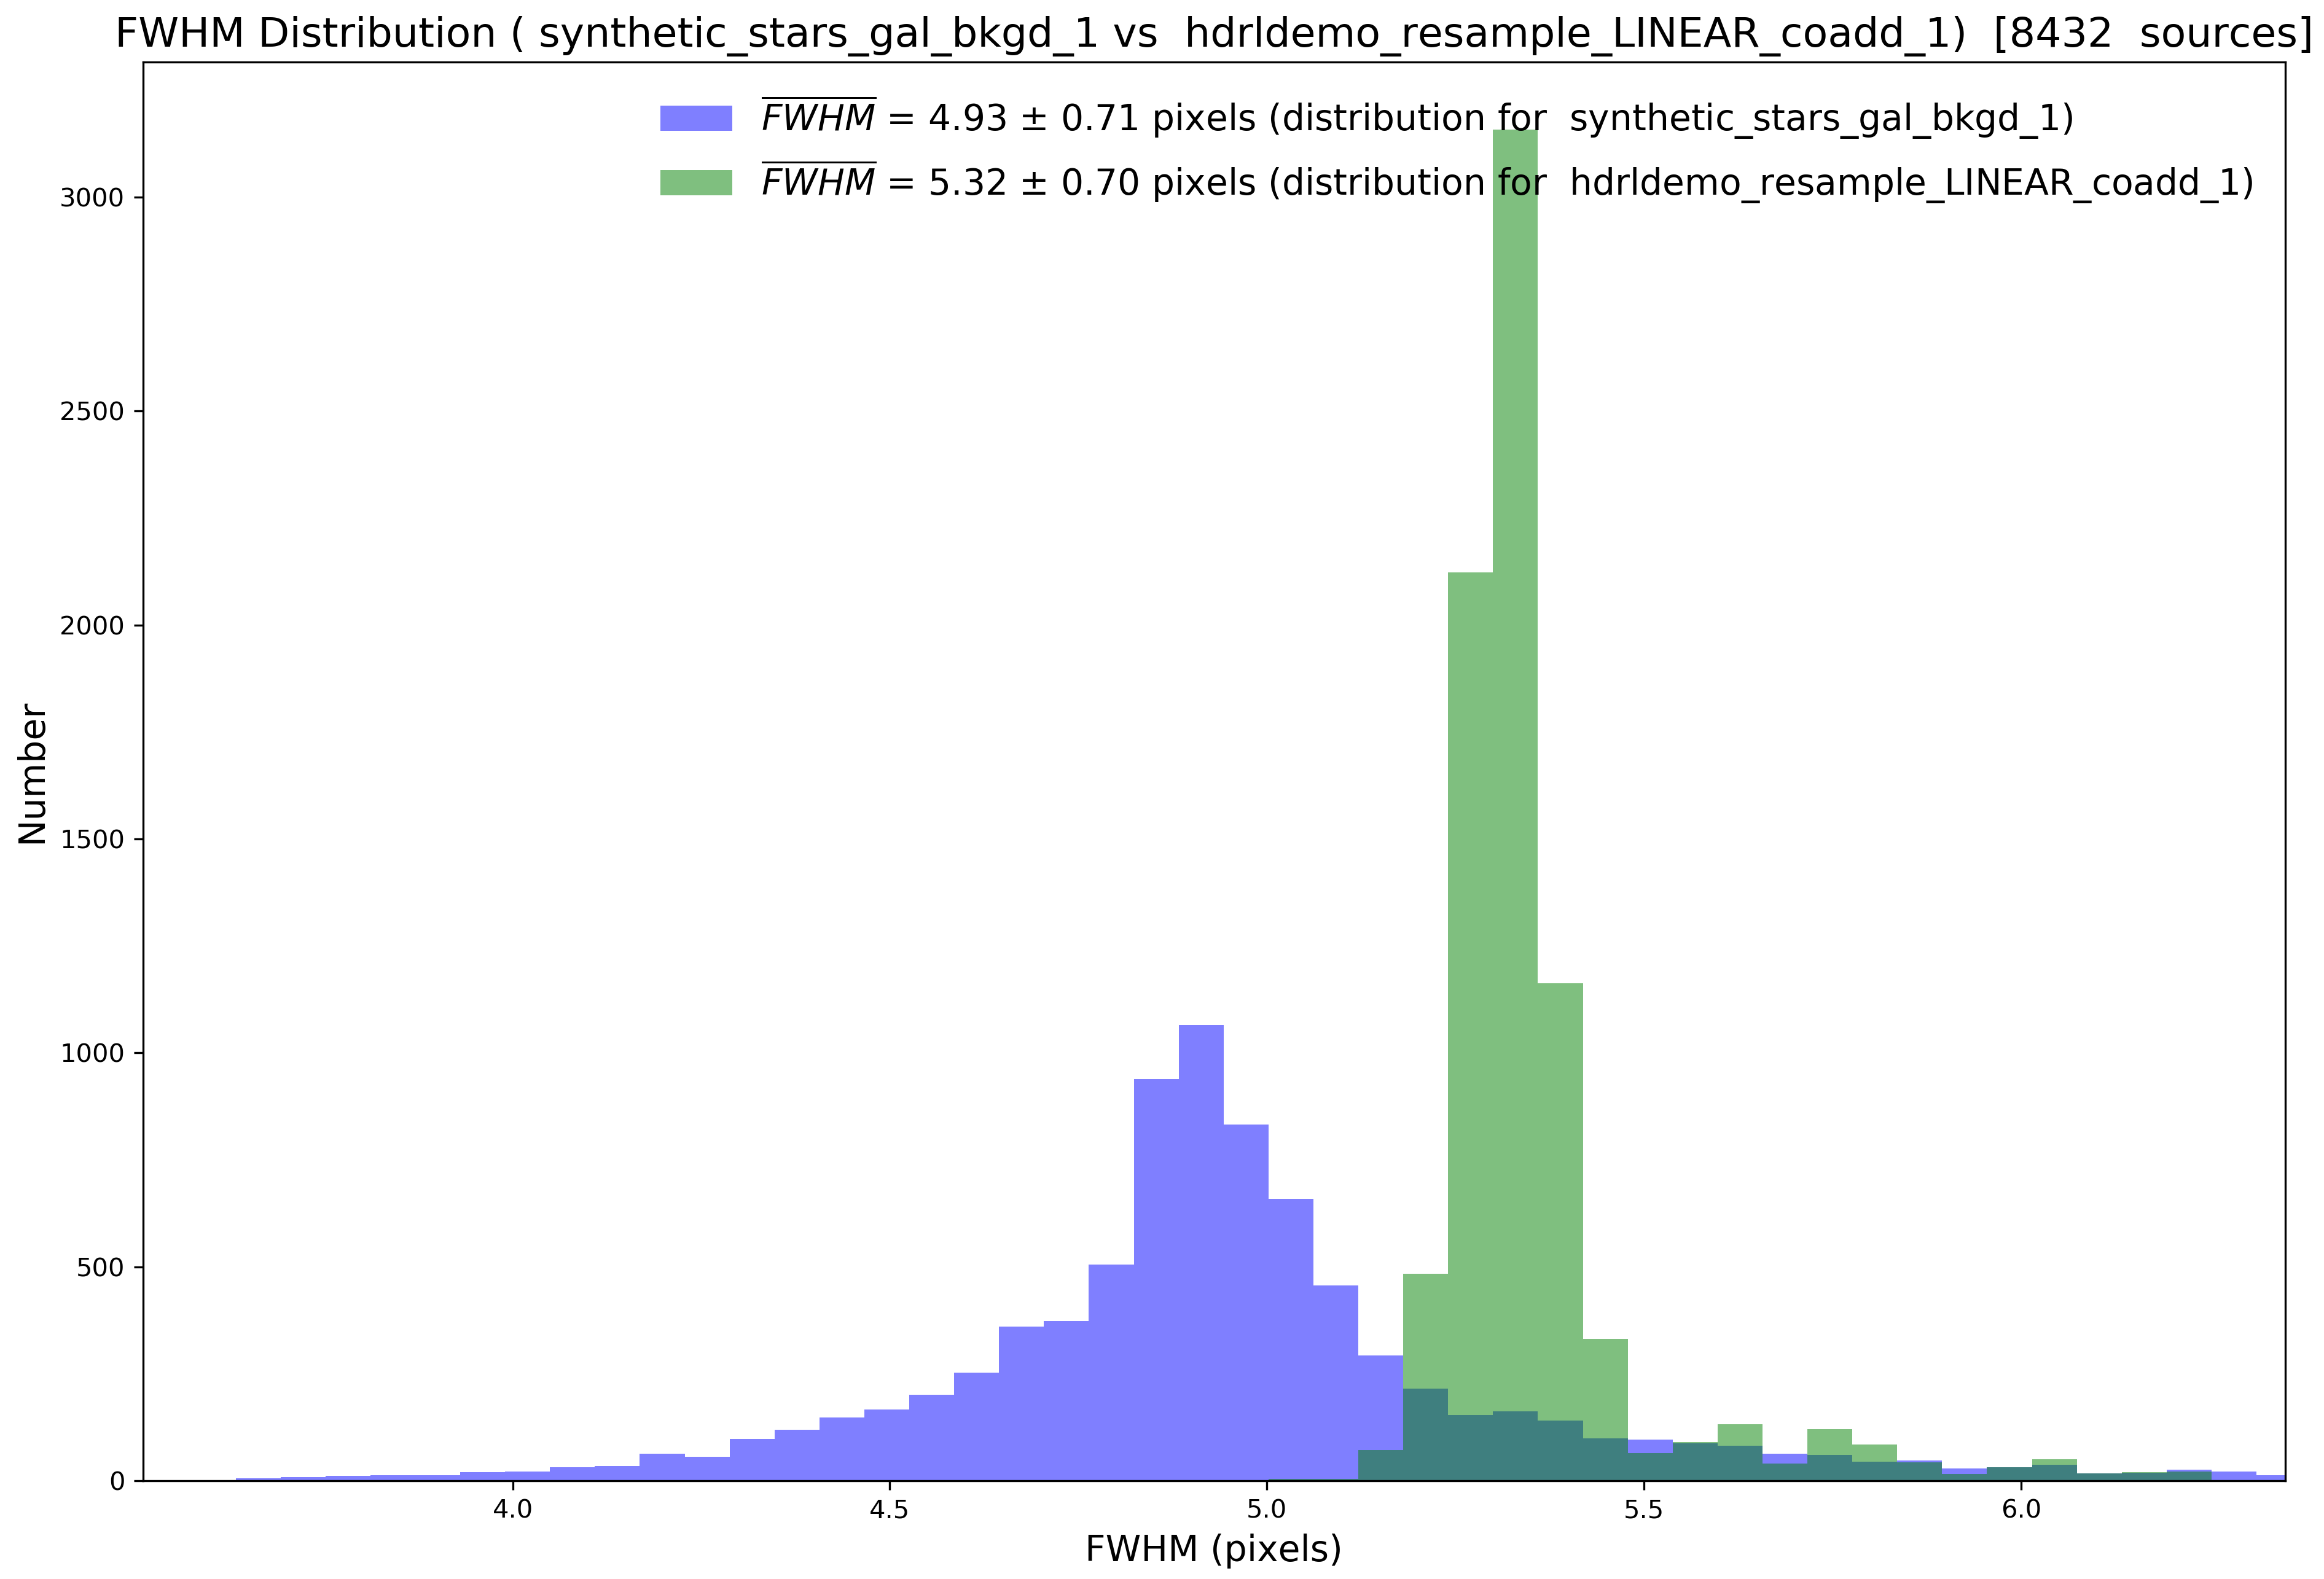
\includegraphics[width=8.4cm]{figures/match_field_LINEAR_coadd_1_FWHM_histogram.png}
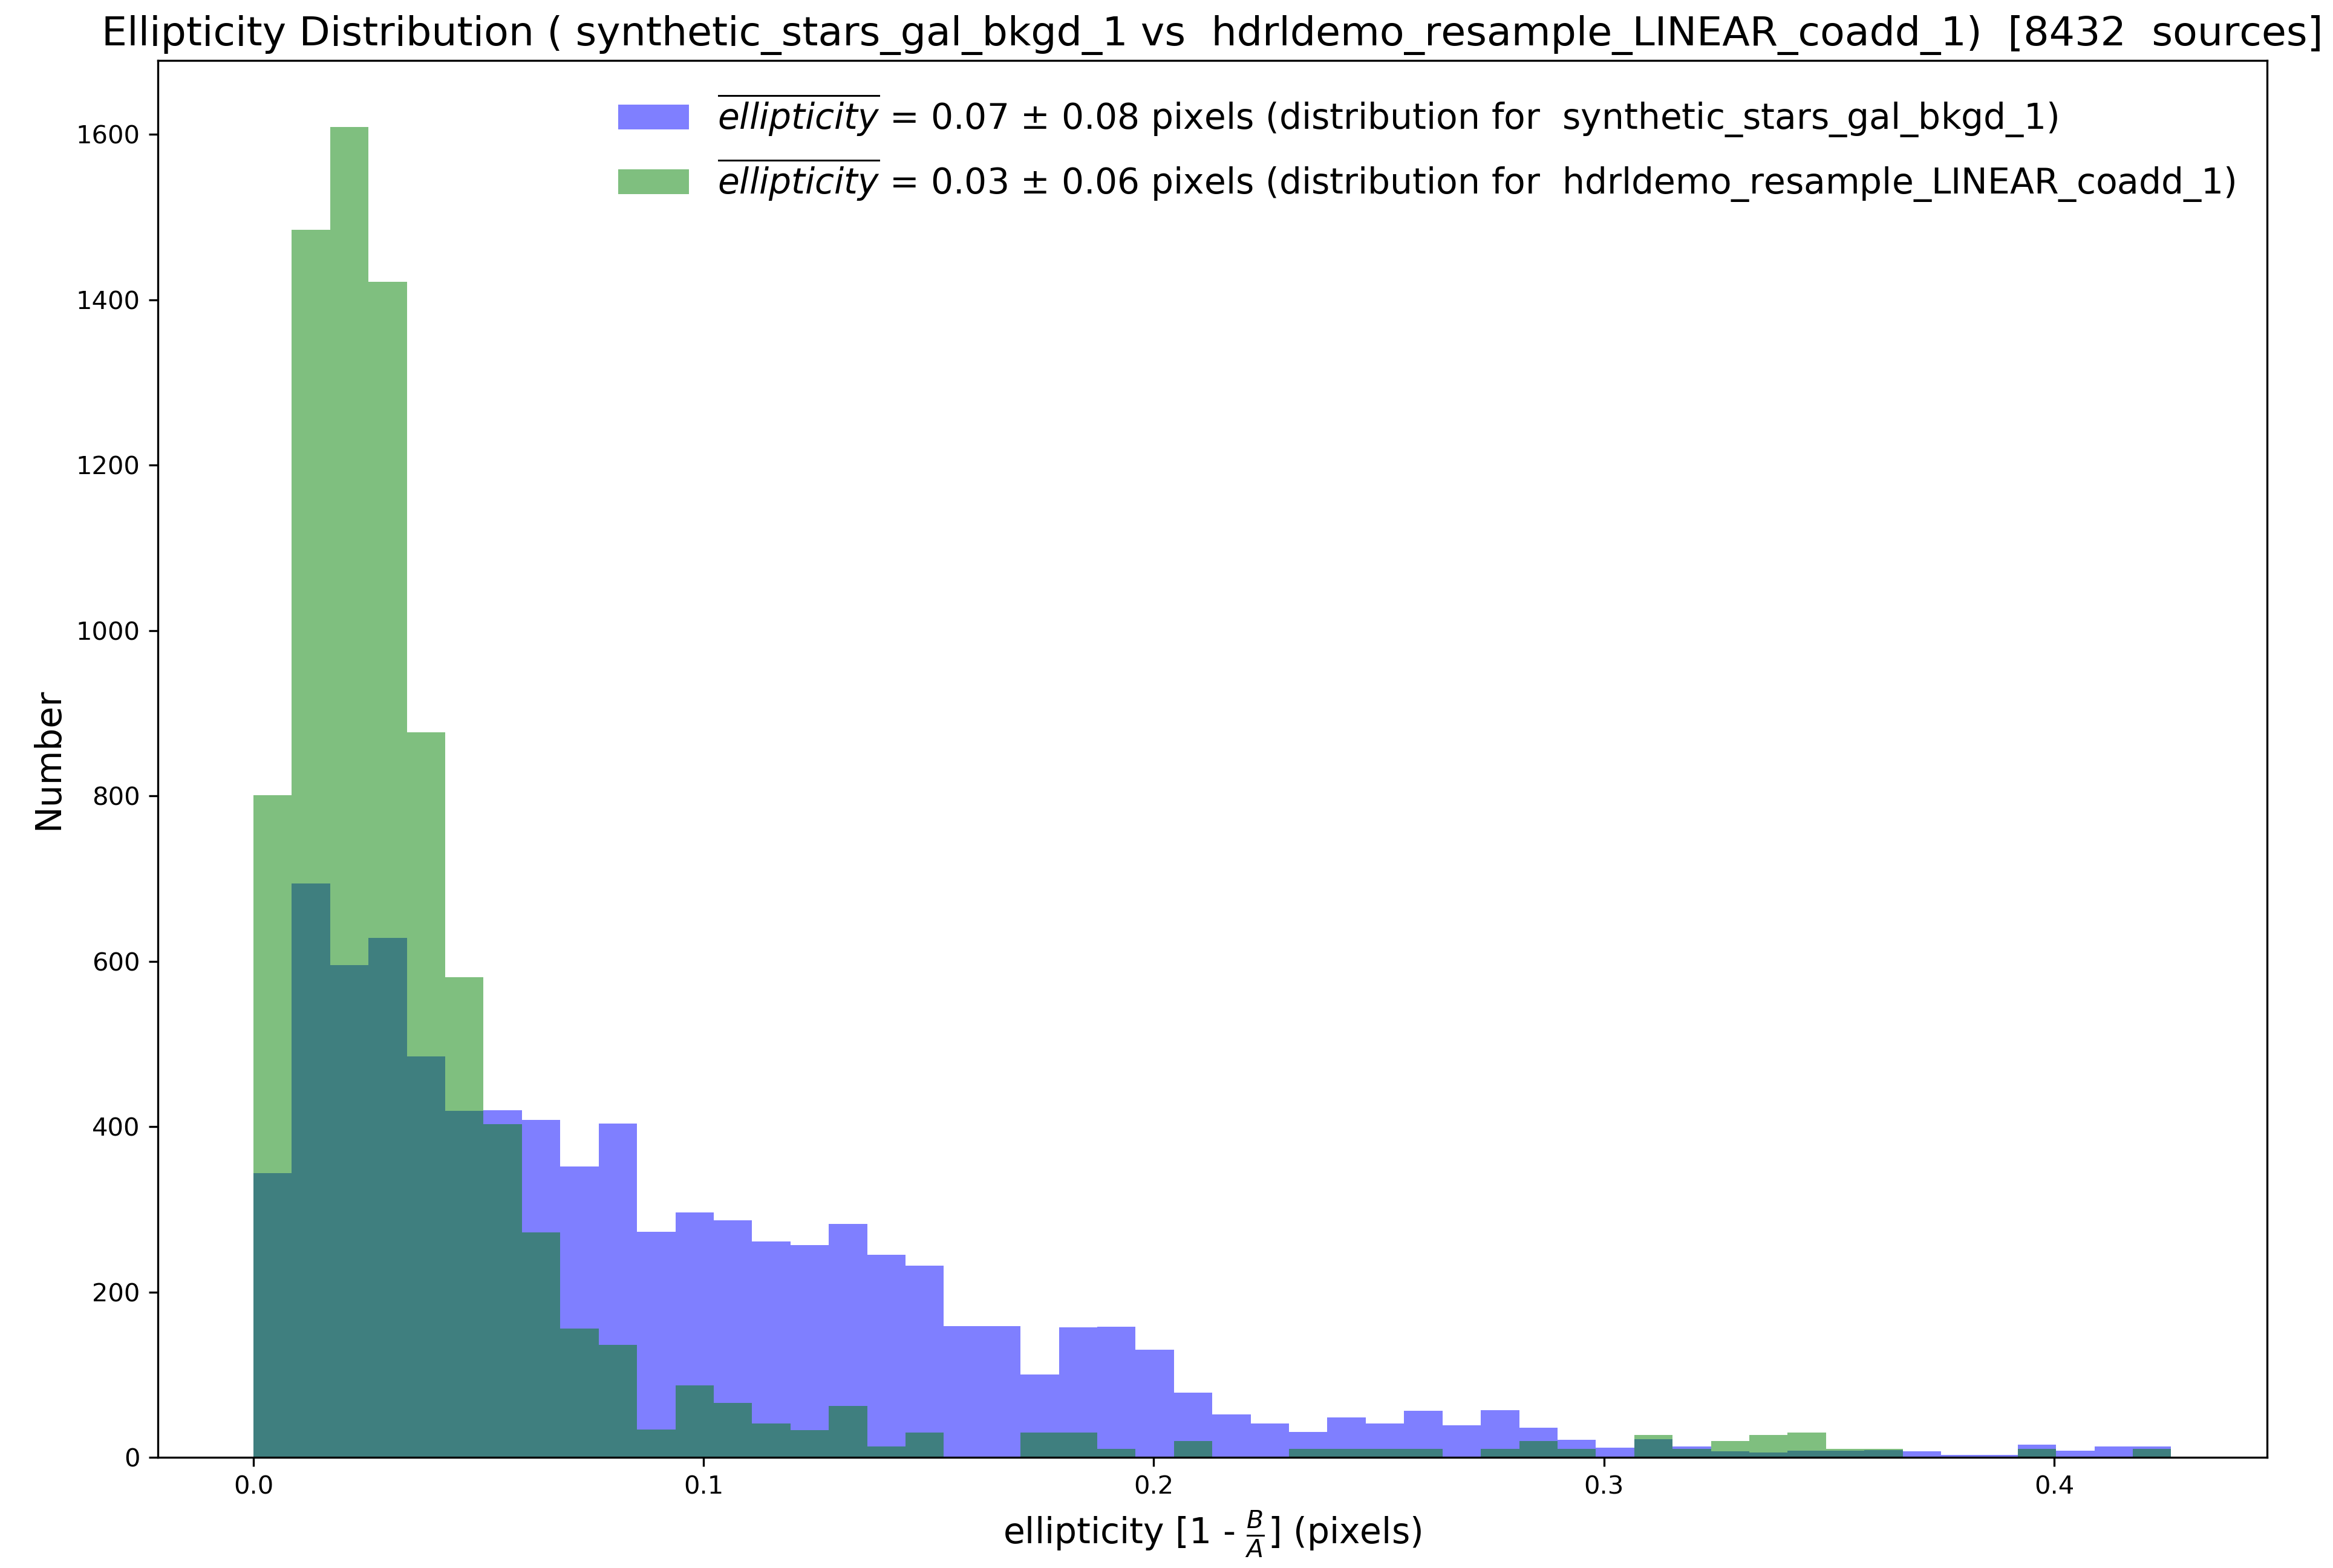
\includegraphics[width=8.4cm]{figures/match_field_LINEAR_coadd_1_ellipticity_histogram.png} 
\caption[]
	{\footnotesize  A comparison of FWHM and ellipticity for the sources in the synthetic input images (blue histograms) and those
	after resampling (green histograms).  The resampling was done with {\tt --method=LINEAR} and {\tt --method.loop-distance=1}.\\
	{\bf left panel:}    The FWHM distribution of the 8,000 sources in the synthetic field. As expected, the median FWHM, after resampling, increases slightly.  
	                          The increase in FWHM is less than 8\%.\\
	{\bf right panel:} The distribution of ellipticities.   Here, the resampling has circularised the sources.   This, too, is as expected. 
	}
	\label{fig:fwhm_ellip_synthetic}
\end{figure}




A summary of the source attributes between the input frames and the resampled images is given in Table \ref{tab:compare_synthetic}, in which the source
attributes of all six resampling methods are compared for both a single synthetic image input and a resampling of 10 synthetic images.

The largest change in the average position of the sources is $\Delta\alpha$=0.1 arcsec and $\Delta\delta$=-0.008 arcsec for the resampling {\tt method=NEAREST}.
Since this is still only one half of a pixel, this is still acceptable.  The largest change in the average magnitude  can be found in the {\tt LINEAR} resampling and
corresponds to a small shift of $\Delta$mag. = 0.06 magnitudes.
The largest change in FWHM is seen for {\tt method=LINEAR}, in which the FWHM of the synthetic
stars increase by 1.8 pixels (37\%).    A measure of the source ellipticities shows a congruent feature.   In all resampling methods the ellipticities are decreased and the distribution is
tightened, as the interpolation has the general effect of circularising the source images.  



\begin{sidewaystable}

\caption{A Summary of Comparisons Between Input Synthetic Data Images and Resultant Interpolation Images}
\footnotesize
\begin{center}
\begin{tabular}{|l|l|c|c|c|c|c|c|c|c|c|c|}                      
\toprule
synthetic\_image         				     & Interpolation	 & N$_{frames}^2$   & Nmatch & $\Delta\alpha$  & $\Delta\delta$ &  $\Delta(mag)$ & $\sigma\Delta(mag)$ & FWHM1$^3$  & FWHM2$^4$  & ellip1$^3$  & ellip2$^4$  \\
                                     & method (LD)$^1$ &                         &               & (arcsec)            & (arcsec)          &                          &                                   & (pixels)    & (pixels)   &            & \\
\midrule
synthetic\_stars\_gal\_bkgd\_single                 & DRIZZLE (1)        & single   	& 893 	& 0.000       & -0.007  	& -0.005 & 0.014          & 4.92  & 4.92  		& 0.07  & 0.07  \\
synthetic\_stars\_gal\_bkgd\_single 	   	       & DRIZZLE (3)        & single  	& 893 	& 0.000       & -0.007  	& -0.005 & 0.014 	   & 4.92  & 4.92  		& 0.07  & 0.07  \\
synthetic\_stars\_gal\_bkgd\_single 	               & LANCZOS (1)      & single  	& 892 	& 0.000       & -0.003  	& -0.005 & 0.016          & 4.92  & 4.92  		& 0.07  & 0.07    \\
synthetic\_stars\_gal\_bkgd\_single 	   	      & LANCZOS (3)      & single  	& 892 	& 0.000       & -0.004  	& -0.005 & 0.015          & 4.92  & 4.92 		& 0.07  & 0.07    \\
synthetic\_stars\_gal\_bkgd\_single 	              & LINEAR (1)          & single    	& 895 	& 0.000       & -0.007  	&  0.003 & 0.026          & 4.92  & 5.03  		& 0.07  & 0.07    \\
synthetic\_stars\_gal\_bkgd\_single 	              & LINEAR (3)          & single    	& 892 	& 0.000       & -0.006  	&  0.020 & 0.041          & 4.92  & 5.64  		& 0.07  & 0.06    \\
synthetic\_stars\_gal\_bkgd\_single 	              & NEAREST (1)      & single   	& 893 	& 0.000       & -0.007  	& -0.005 & 0.014          & 4.92  & 4.92  		& 0.07  & 0.07    \\
synthetic\_stars\_gal\_bkgd\_single 	              & NEAREST (3)      & single   	& 893 	& 0.000       & -0.007  	& -0.005 & 0.014          & 4.92  & 4.92  		& 0.07  & 0.07    \\
synthetic\_stars\_gal\_bkgd\_single 	              & QUADRATIC (1)  & single 	& 890 	& 0.000       & -0.007  	& -0.004 & 0.015          & 4.92  & 4.92  		& 0.07  & 0.07    \\
synthetic\_stars\_gal\_bkgd\_single 	              & QUADRATIC (3)  & single 	& 889 	& 0.000       & -0.007  	& -0.004 & 0.015          & 4.92  & 4.93   		& 0.07  & 0.07    \\
synthetic\_stars\_gal\_bkgd\_single 	              & RENKA (1)           & single 	& 892 	& 0.000       & -0.007  	& -0.005 & 0.015          & 4.92  & 4.92 		& 0.07  & 0.07   \\
synthetic\_stars\_gal\_bkgd\_single                & RENKA (3)           & single  	& 892 	& 0.000       & -0.007  	& -0.004 & 0.014          & 4.92  & 4.92  		& 0.07  & 0.07    \\
\midrule
synthetic\_stars\_gal\_bkgd\_1$\to$10   	& DRIZZLE (1)        &10    		&  8,587 	& 0.001       & -0.008  	& 0.024  & 0.06 	& 4.93  & 5.01  			& 0.07    & 0.03  \\
synthetic\_stars\_gal\_bkgd\_1$\to$10   	& DRIZZLE (3)        &10    		&  8,587 	& 0.001       & -0.008  	& 0.024  & 0.06 	& 4.93  & 5.01 			& 0.07    & 0.03  \\
synthetic\_stars\_gal\_bkgd\_1$\to$10   	& LANCZOS (1)      &10    		&  8,619 	& -0.017      & 0.003   	& 0.024  & 0.06		& 4.93  & 4.97  			& 0.07    & 0.03  \\
synthetic\_stars\_gal\_bkgd\_1$\to$10   	& LANCZOS (3)     &10    			&  8,629 	& 0.007       & -0.001  	& 0.020  & 0.06 	& 4.93  & 4.88  			& 0.07    & 0.03  \\
synthetic\_stars\_gal\_bkgd\_1$\to$10   	& LINEAR (1)         &10 	   		&  8,603 	& 0.056       & -0.006  	& 0.040  & 0.07 	& 4.93  & 5.32  			& 0.07    & 0.03  \\
synthetic\_stars\_gal\_bkgd\_1$\to$10   	& LINEAR (3)         &10 	   		&  8,508 	& 0.051       & -0.005  	& 0.064  & 0.07  	& 4.93  & 6.76   		& 0.07    & 0.03  \\
synthetic\_stars\_gal\_bkgd\_1$\to$10   	& NEAREST (1)     &10    			&  8,390 	& 0.099       & -0.008  	&-0.007  & 0.01 	& 4.93  & 4.91 			& 0.07    & 0.07  \\
synthetic\_stars\_gal\_bkgd\_1$\to$10   	& NEAREST (3)     &10    			&  8,390 	& 0.099       & -0.008  	&-0.007  & 0.01 	& 4.93  & 4.91  			& 0.07    & 0.07  \\
synthetic\_stars\_gal\_bkgd\_1$\to$10   	& QUADRATIC (1) &10  			&  8,589 	& 0.027       & -0.005  	& 0.031  & 0.07 	& 4.93  & 5.18  			& 0.07   & 0.03  \\
synthetic\_stars\_gal\_bkgd\_1$\to$10   	& QUADRATIC (3) &10  			&  8,569	& 0.018       & -0.003  	& 0.042  & 0.06 	& 4.93  & 5.74  			& 0.07   & 0.03  \\
synthetic\_stars\_gal\_bkgd\_1$\to$10   	& RENKA (1)          &10 	   		&  8,581 	& 0.006       & -0.005  	& 0.029  & 0.07 	& 4.93  & 5.07  			& 0.07   & 0.03  \\
synthetic\_stars\_gal\_bkgd\_1$\to$10   	& RENKA (3)          &10	   		&  8,581 	& 0.003       & -0.004  	& 0.029  & 0.07 	& 4.93  & 5.08  			& 0.07   & 0.03  \\
\bottomrule


\end{tabular}	
\end{center}																											

\label{tab:compare_synthetic}
\noindent{
		$^1$ The interpolation method and loop-distance used ({\tt --method.loop-distance}).\\
		$^2$ The total number of synthetic input images combined during the resampling.\\
		$^3$ FWHM1 and ellip1 refer to the synthetic input images.\\
		$^4$ FWHM2 and ellip2 refer to the resampled images.}
\end{sidewaystable}

\normalsize

\subsection{Results from HAWK-I Globular Cluster Images}
\label{sect:hawki1}


To test the \hdrlresample\ routines a series of large-field HAWK-I exposures were processed.  
This data includes the globular cluster fields mapping M30 and NGC288.
The data for M30 is from 2015-10-31 with OBS.ID=200203309, while the data for NGC288 is from 2016-11-22 with OBS.ID=200203307.
Both data sets have PROG.ID=60.A-9800(L).

All data has been processed using the HAWK-I pipeline version 2.4.6, with the intermediate pipeline science products 
({\tt BASIC\_CALIBRATED\_SCI} and {\tt BASIC\_VAR\_MAP}) acting as input for the \hdrlint\  and image combination routines.
Each data set consisted of 25, calibrated science frames (dark-corrected, gain-corrected, flat-fielded, and astrometrically and photometrically calibrated), with each being a MEF
of four detectors for a total of 100 individual exposures.
These 100 images were resampled using each of the methods available in \hdrlresample, {\tt NEAREST, LINEAR, QUADRATIC, RENKA, LANCZOS,
and DRIZZLE}, and each was executed with both a loop distance of 1 and 3 pixels ({\tt --method.loop-distance}).
The resulting image tiles are then compared to the original input images.

The comparison of the data products is done using a python script ({\tt compare\_image\_sex.py}).  This script runs SExtractor (\cite{bertin})
on both images with a {\tt -DETECT\_THRESH} and {\tt -ANALYSIS\_THRESH} of 5.0\,$\sigma$ and a {\tt -DETECT\_MINAREA} of 10 pixels.
A spherical, nearest-neighbour match within 1 arcsec is then done between the sources of the two resultant SExtractor catalogues.
This allows us to compare the attributes (position ($\alpha, \delta$), magnitude, FWHM, and ellipticity) of the ensemble of extracted sources
from the original input images to the same sources once they have been resampled by each of the six interpolation methods.


% NGC288:
\subsubsection{NGC288}

An example of the \hdrlresample\ product is shown in figure \ref{fig:hawki_ngc288}.  A comparison with the combined frames from the
HAWK-I pipeline (combined with {\tt hawki\_science\_postprocess} show qualitatively very similar results.


\begin{figure}[H]
\centering
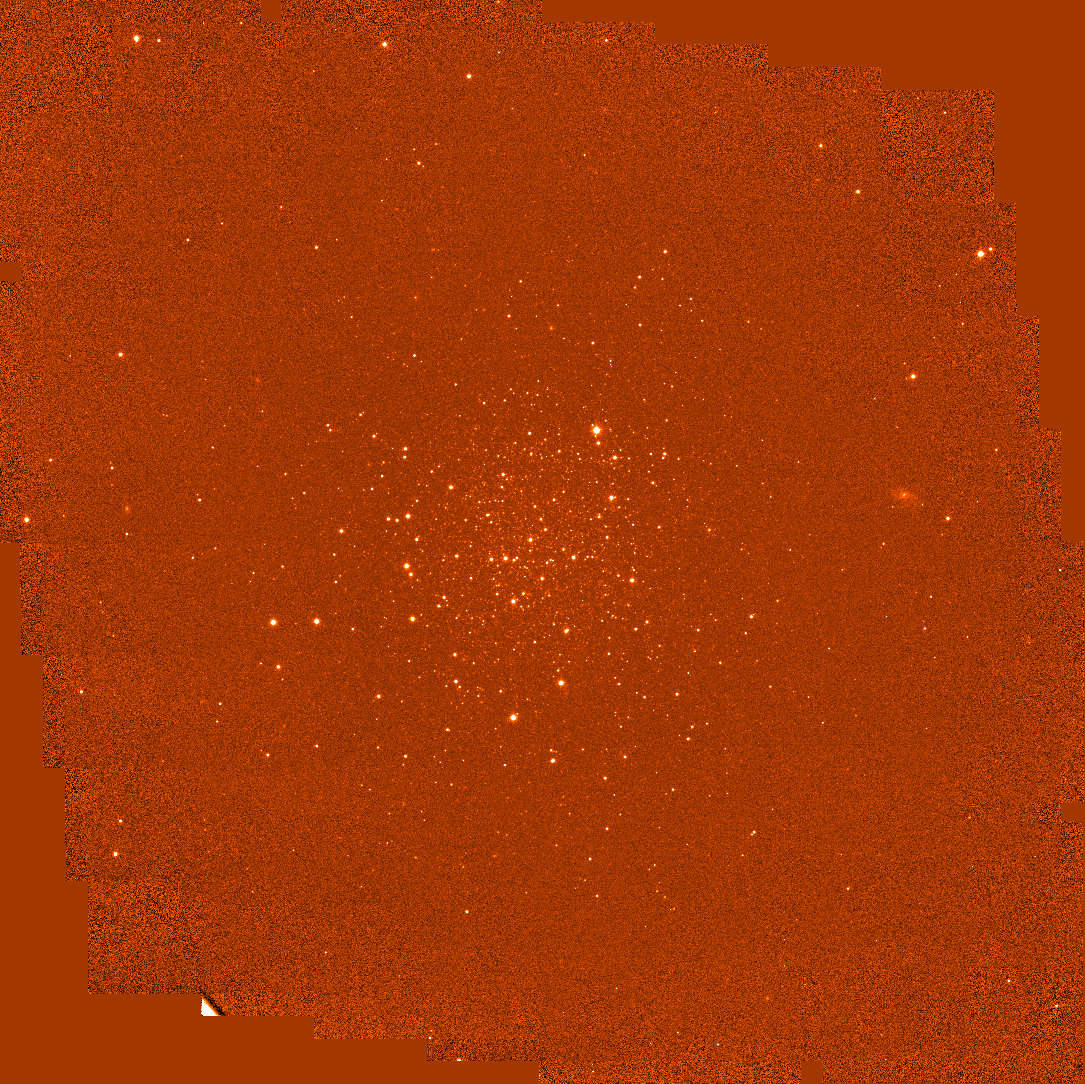
\includegraphics[width=8.4cm]{figures/Distortion_NGC288_TILED_IMAGE.png}
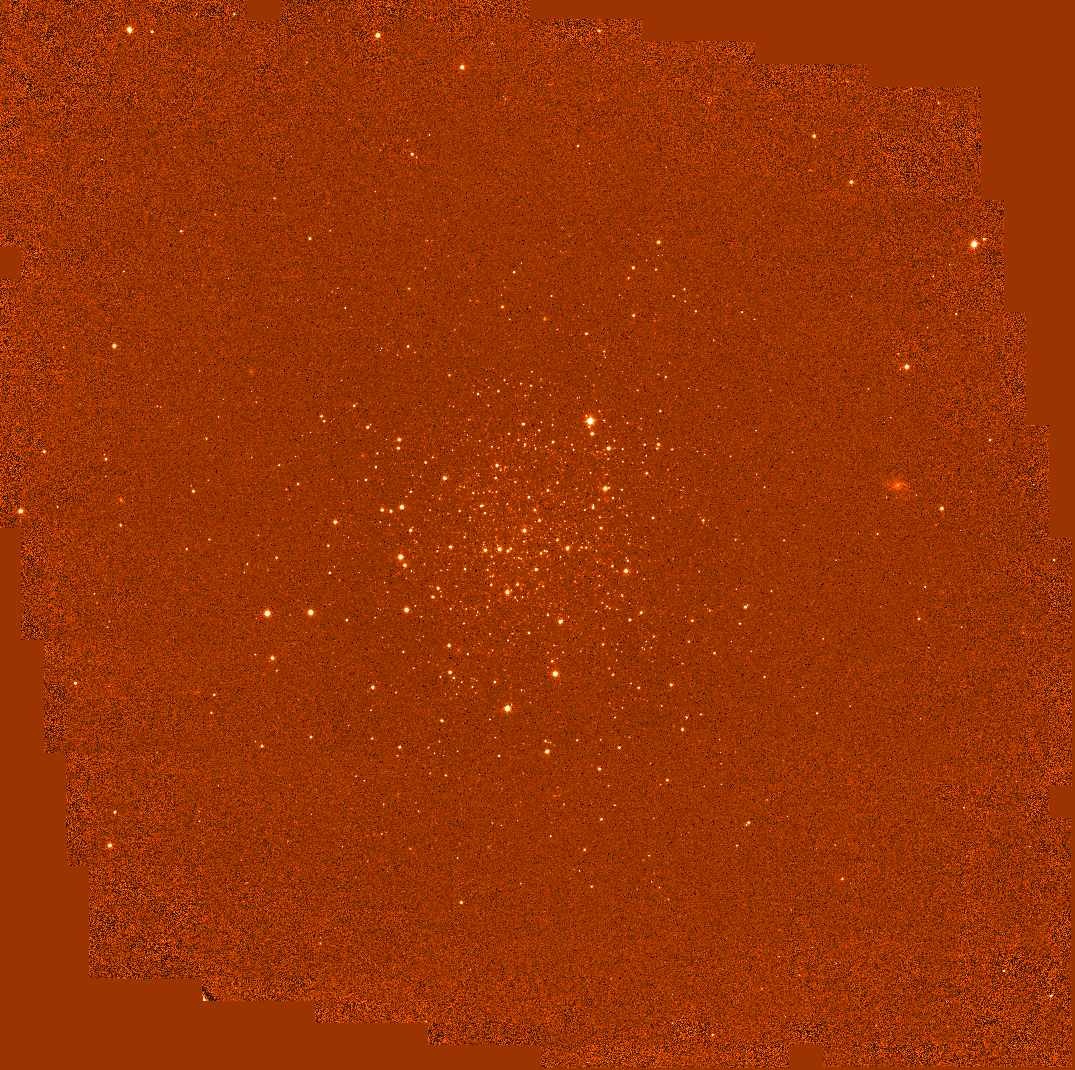
\includegraphics[width=8.4cm]{figures/hdrldemo_resample_DRIZZLE_HAWKI_NGC288_1.png} 
\caption[]
	{\footnotesize  The final tile image made from 100 HAWK-I images of the NGC\,288 field:\\
	{\bf left panel:}    as creating by the HAWK-I pipeline v. 2.4.6 routine {\tt hawki\_science\_postprocess}\\
	{\bf right panel:} as resampled and combined using \hdrlresample\ with {\tt --method=DRIZZLE} and {\tt --method.loop-distance=1}.\\
	}
	\label{fig:hawki_ngc288}
\end{figure}

In all five methods of image resampling, the astrometric quality of the sources is retained following interpolation.  An example of this is shown in 
figure \ref{fig:radec_NGC288}.  Here, the absolute positions of the sources in the 100 input HAWK-I images is compared to the absolute positions
of the sources in the image resample using the drizzle method.   Here, the median $\Delta\alpha*\cos(\delta)=0.001\pm0.07\ arcsec$ and 
$\Delta\delta=0.003\pm0.07\ arcsec$ with the cloud of offsets spread symmetrically about the origin.  
Considering that the HAWK-I pixel size is 0.106 pixels/arcsec, the astrometric accuracy is retained to better than a fraction of one pixel (0.66 pixels).

\begin{figure}[H]
\centering
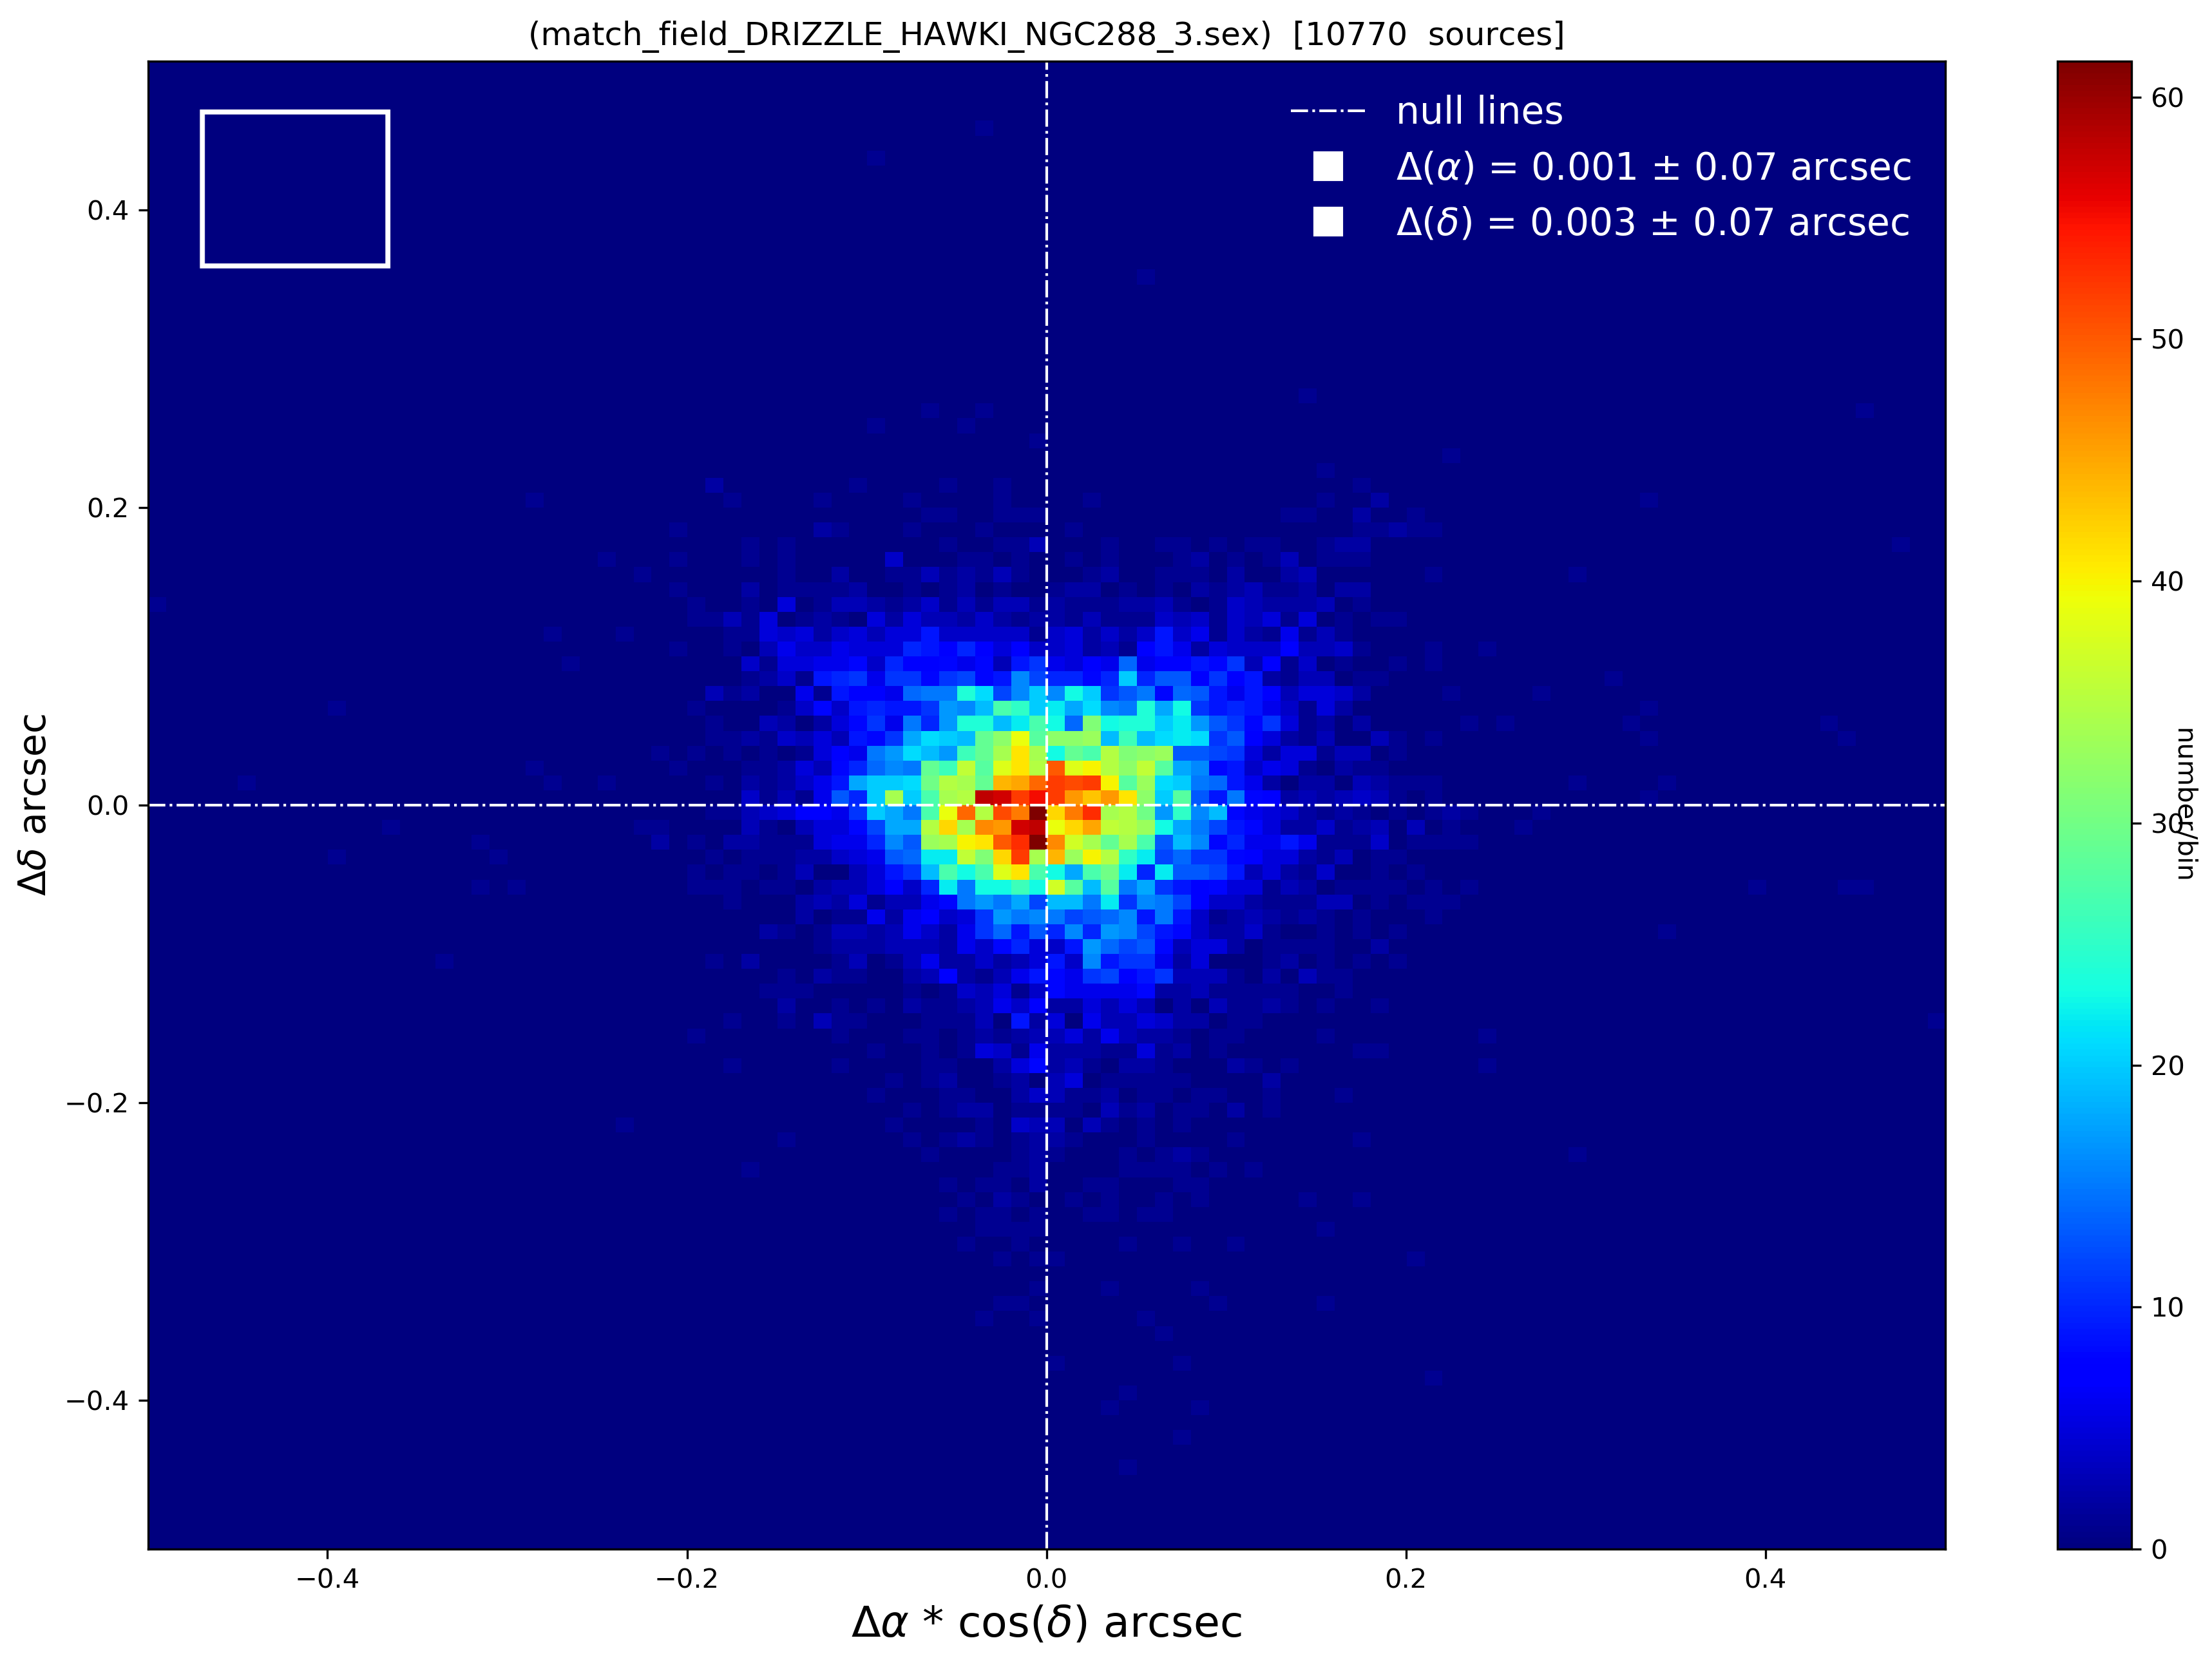
\includegraphics[width=11cm]{figures/match_field_DRIZZLE_HAWKI_NGC288_3_RA_DEC_scatter_plot.png}
\caption[]
	{\footnotesize  the astrometric quality of the \hdrlresample\ routines as measured by comparing the more than 10,000 sources in original input HAWK-I images
	with those in the resampled (drizzle) image tile of Figure \ref{fig:hawki_ngc288}.
	The standard deviation of the $\Delta\alpha*\cos(\delta)$ and $\Delta\delta$ distributions is 0.07 arcsec. This is significantly less than one HAWK-I
	pixel (0.106 pixels/arcsec).  The pixel size is indicated by the white square in the top left corner.
	}
	\label{fig:radec_NGC288}
\end{figure}


\begin{figure}[H]
\centering
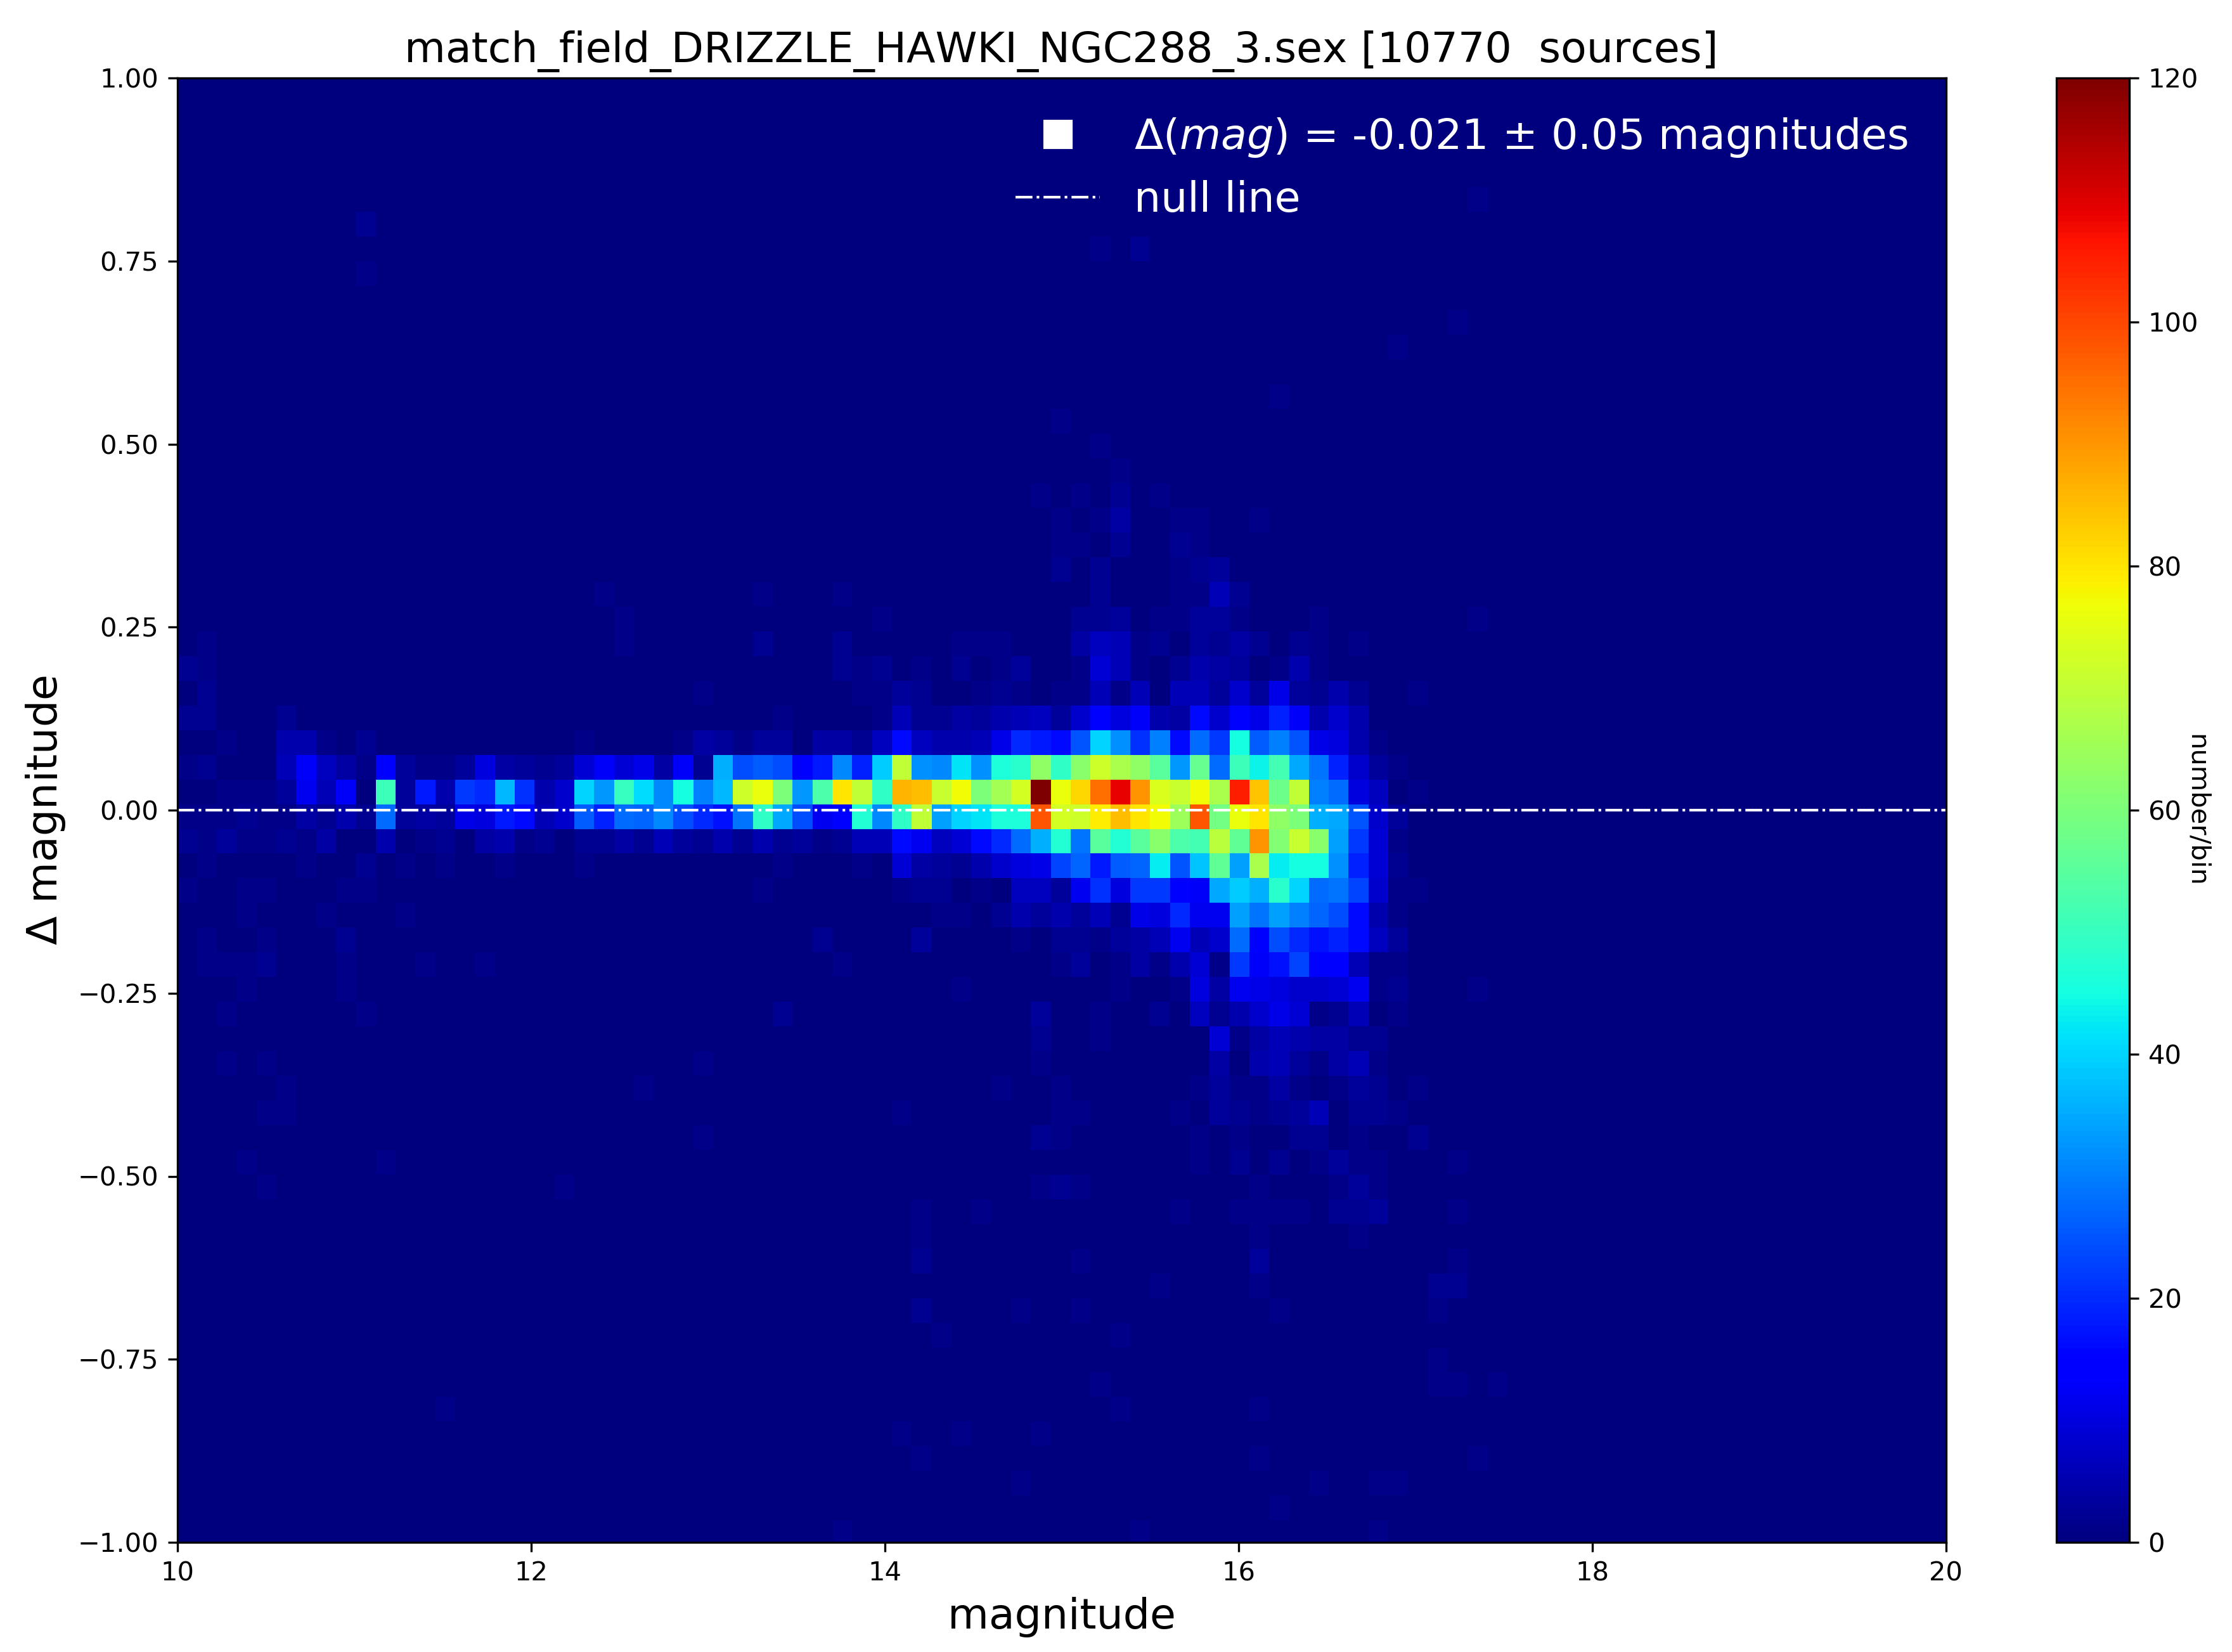
\includegraphics[width=11cm]{figures/match_field_DRIZZLE_HAWKI_NGC288_3_mag_scatter_plot.png}
\caption[]
	{\footnotesize  the photometric quality of the \hdrlresample\ routines as measured by comparing the more than 10,000 sources in original input HAWK-I images
	with those in the resampled (drizzle) image tile of Figure \ref{fig:hawki_ngc288} (right panel).
	The standard deviation of the $\Delta(mag)$  distribution is 0.05 magnitudes. 	
	}
	\label{fig:mag_NGC288}
\end{figure}

Similarly, the photometric quality is also retained following interpolation.   Figure \ref{fig:mag_NGC288} is typical of all interpolated frames, with a source magnitude match 
between the individual HAWK-I images and the resampled (drizzle) image tile of $\Delta(mag)=-0.02\pm0.05$ magnitudes.

As can be seen in figure \ref{fig:fwhm_ellip_NGC288}, the resampling causes a slight increase in the FWHM of the sources and a decrease in the source ellipticities.
This is expected, since the resampling will cause a circularisation and homogenisation of the source shapes.


\begin{figure}[H]
\centering
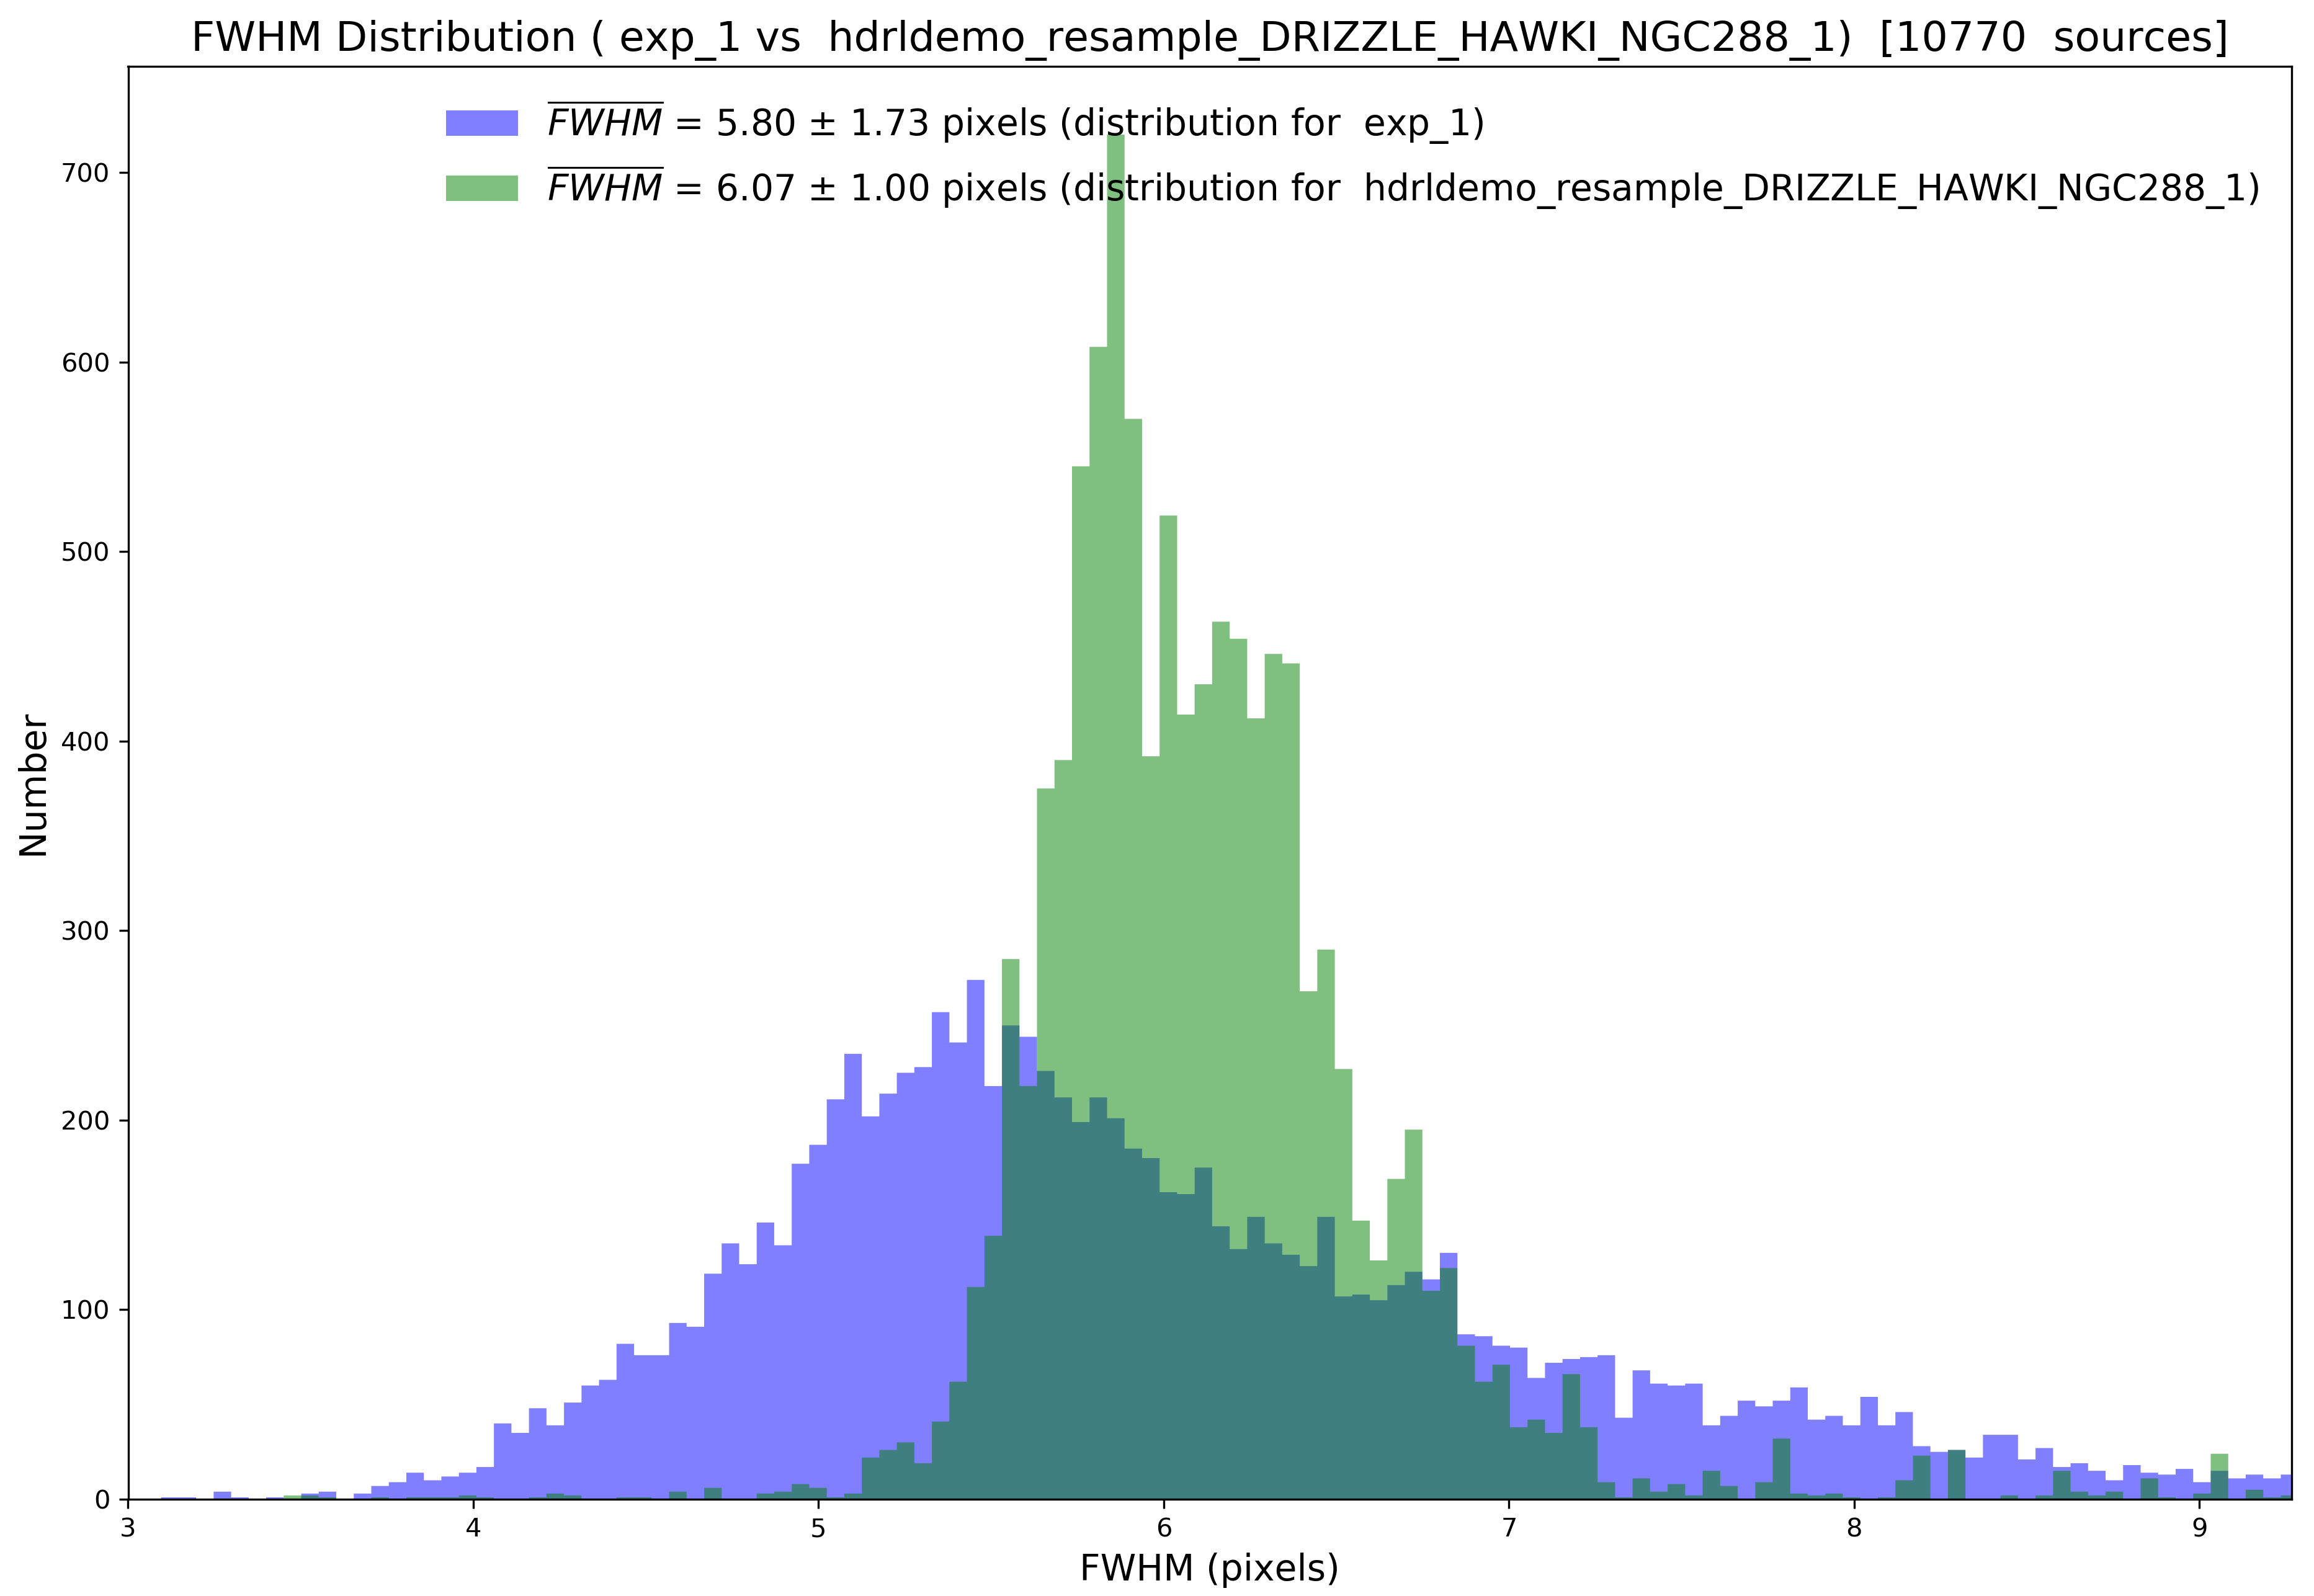
\includegraphics[width=8.4cm]{figures/match_field_DRIZZLE_HAWKI_NGC288_1_FWHM_histogram.png}
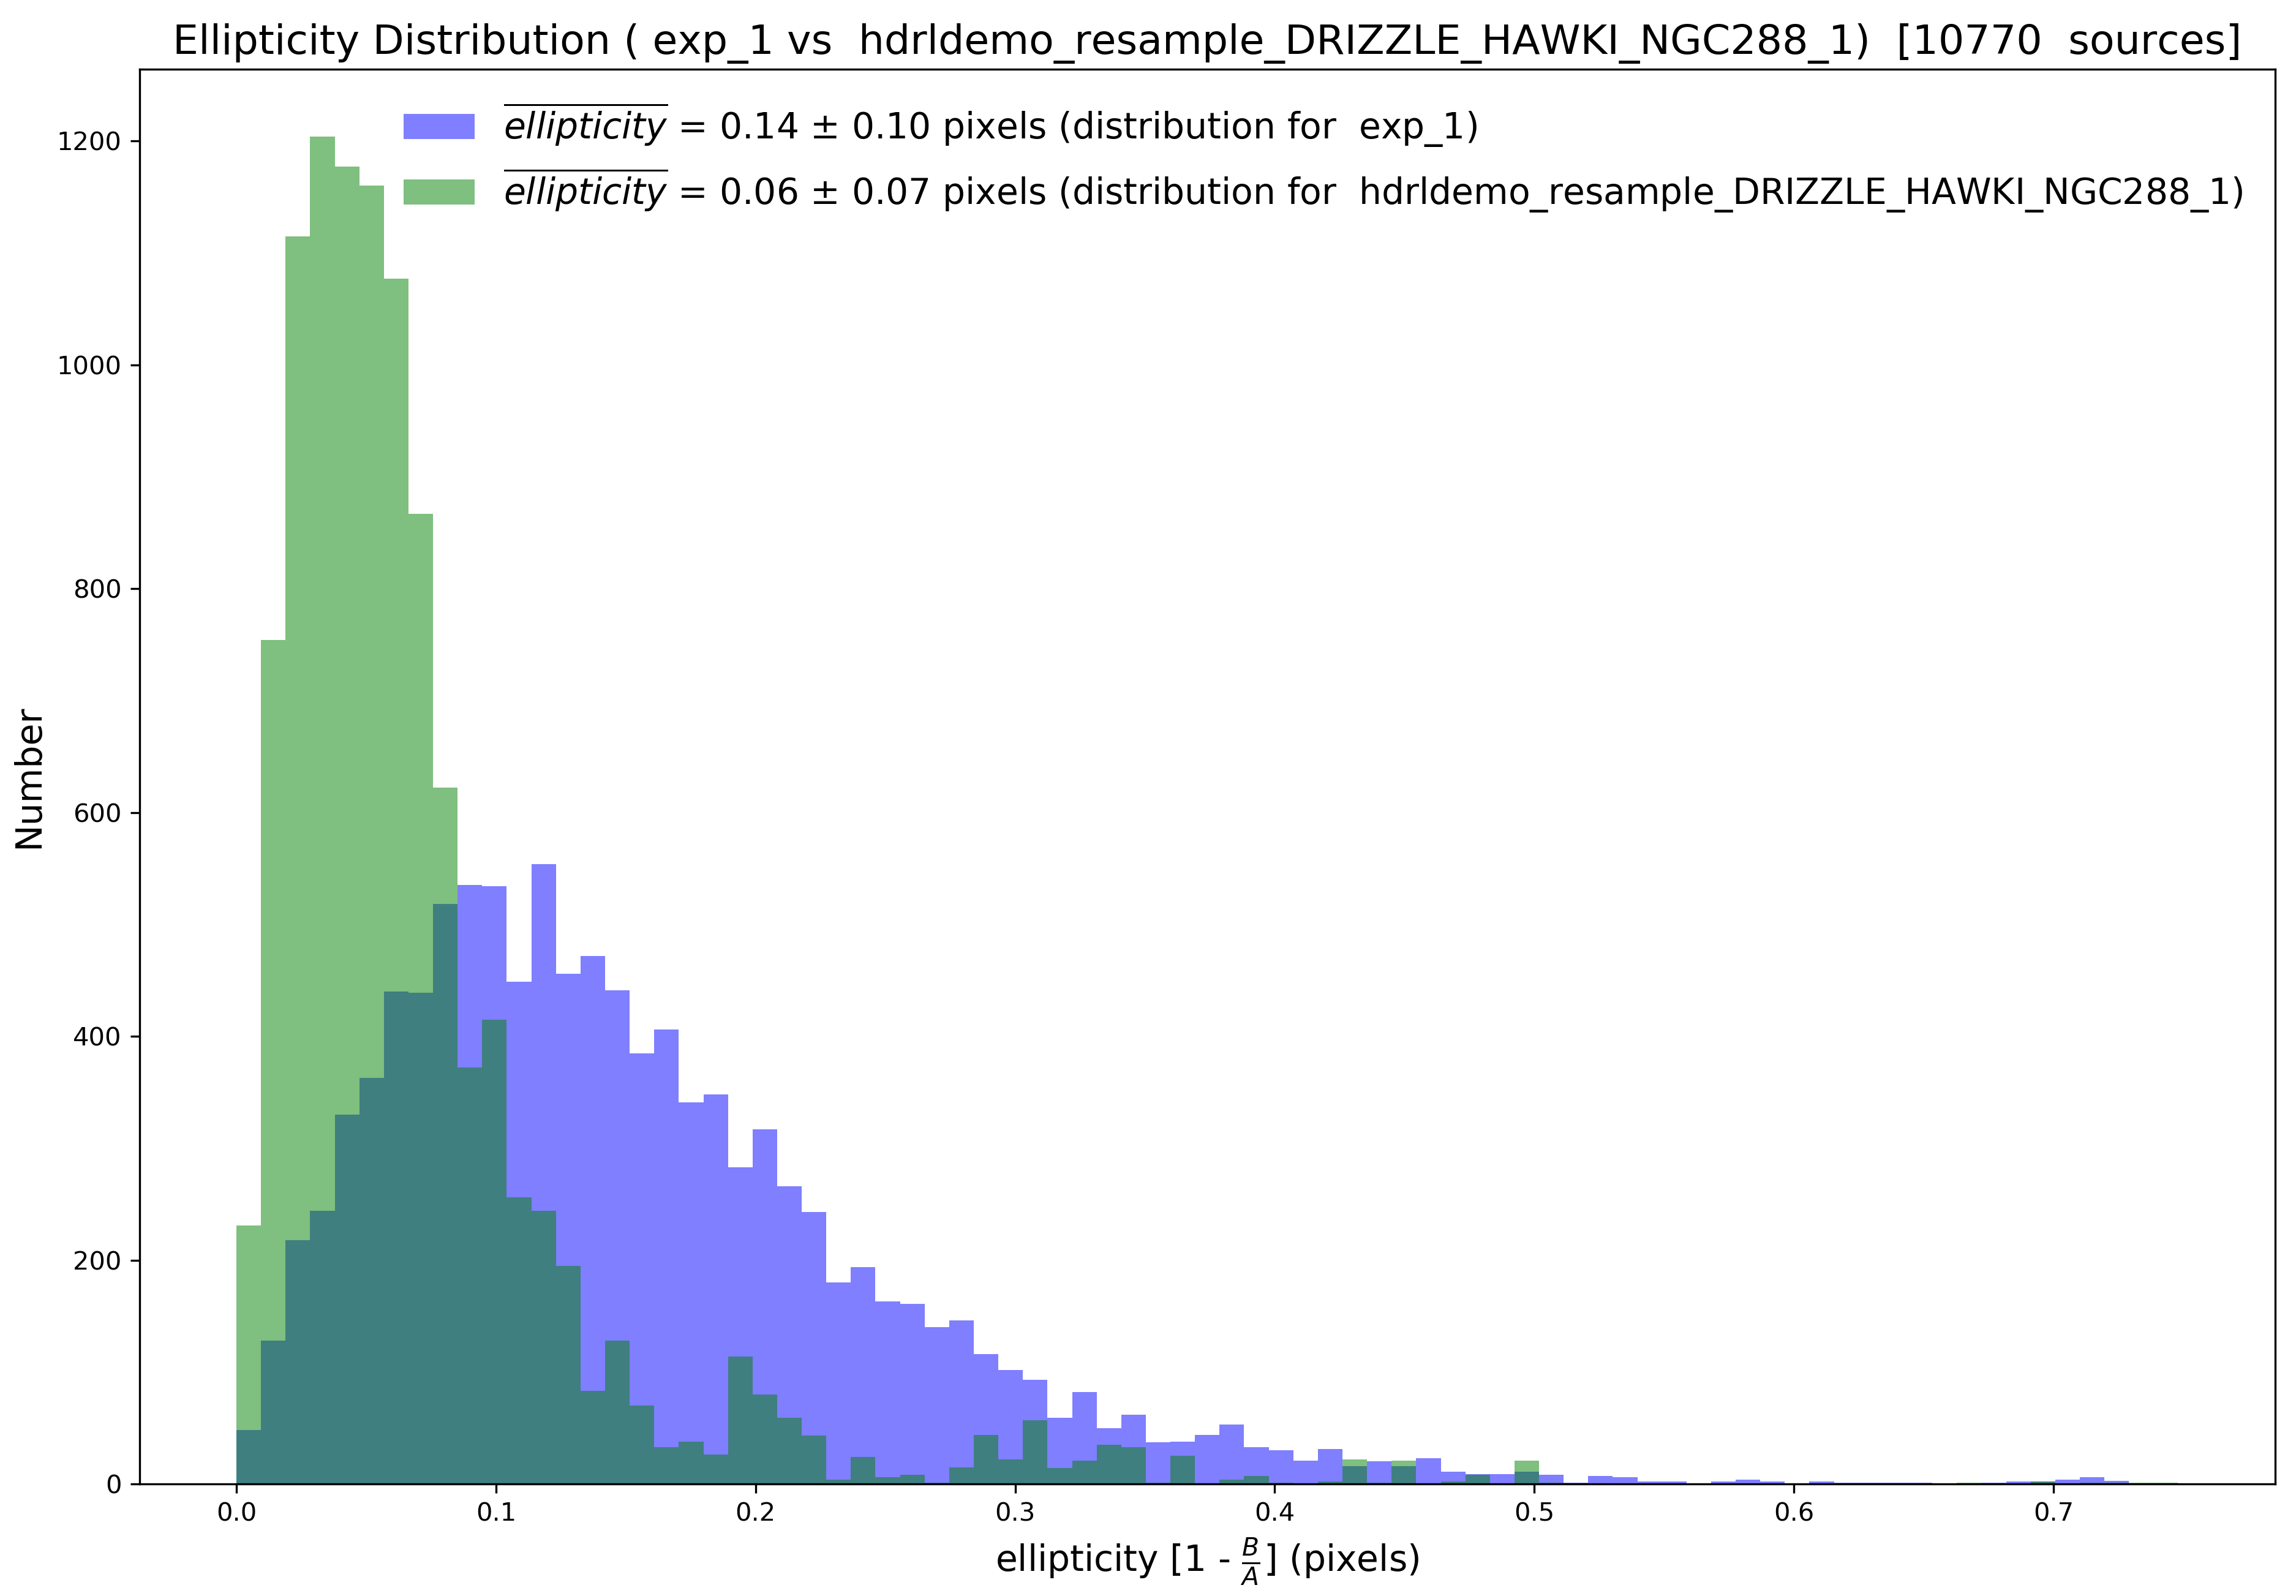
\includegraphics[width=8.4cm]{figures/match_field_DRIZZLE_HAWKI_NGC288_1_ellipticity_histogram.png} 
\caption[]
	{\footnotesize  A comparison of FWHM and ellipticity for the sources in the HAWK-I input images (blue histograms) and those
	after resampling (green histograms).  The resampling was done with {\tt --method=DRIZZLE} and {\tt --method.loop-distance=1}.\\
	{\bf left panel:}    The FWHM distribution of the 10,000 sources in the NGC288 field. As expected, the median FWHM, after resampling, increases slightly.  
	                           Since the increase in FWHM is less than 5\%, this is acceptable.\\
	{\bf right panel:} The distribution of ellipticities.   Here, the resampling has circularised the sources.   This, too, is as expected. 
	}
	\label{fig:fwhm_ellip_NGC288}
\end{figure}



%  
%  M30:
\subsubsection{M30}

The analysis of the denser globular cluster M30 shows similar good results when the individual input HAWK-I images are compared to the
resampled results.   An example of the \hdrlresample\ product ({\tt --method=DRIZZLE} and {\tt --method.loop-distance=1})
is shown in figure \ref{fig:hawki_M30}.  

\begin{figure}[H]
\centering
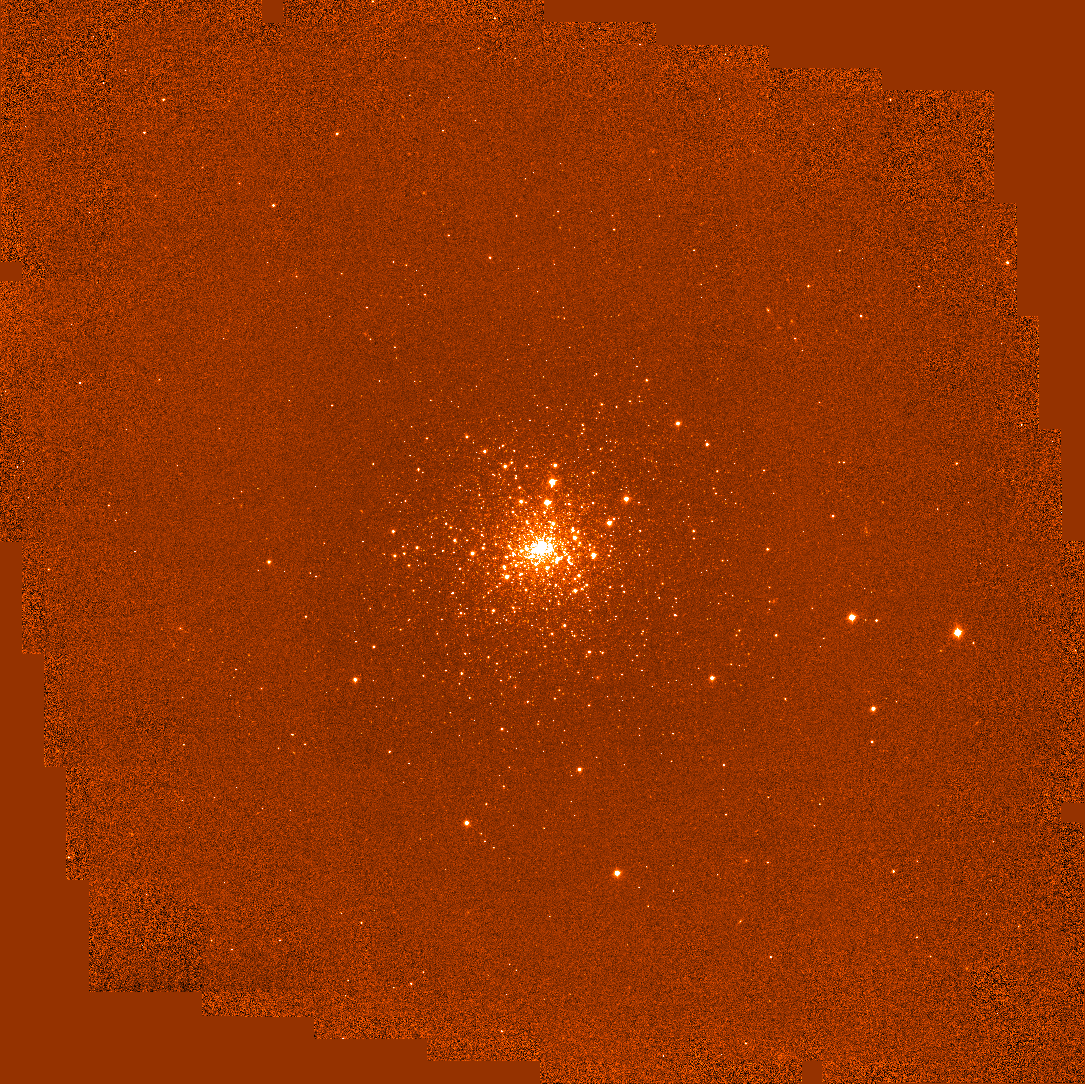
\includegraphics[width=8.4cm]{figures/Distortion_M30_TILED_IMAGE.png}
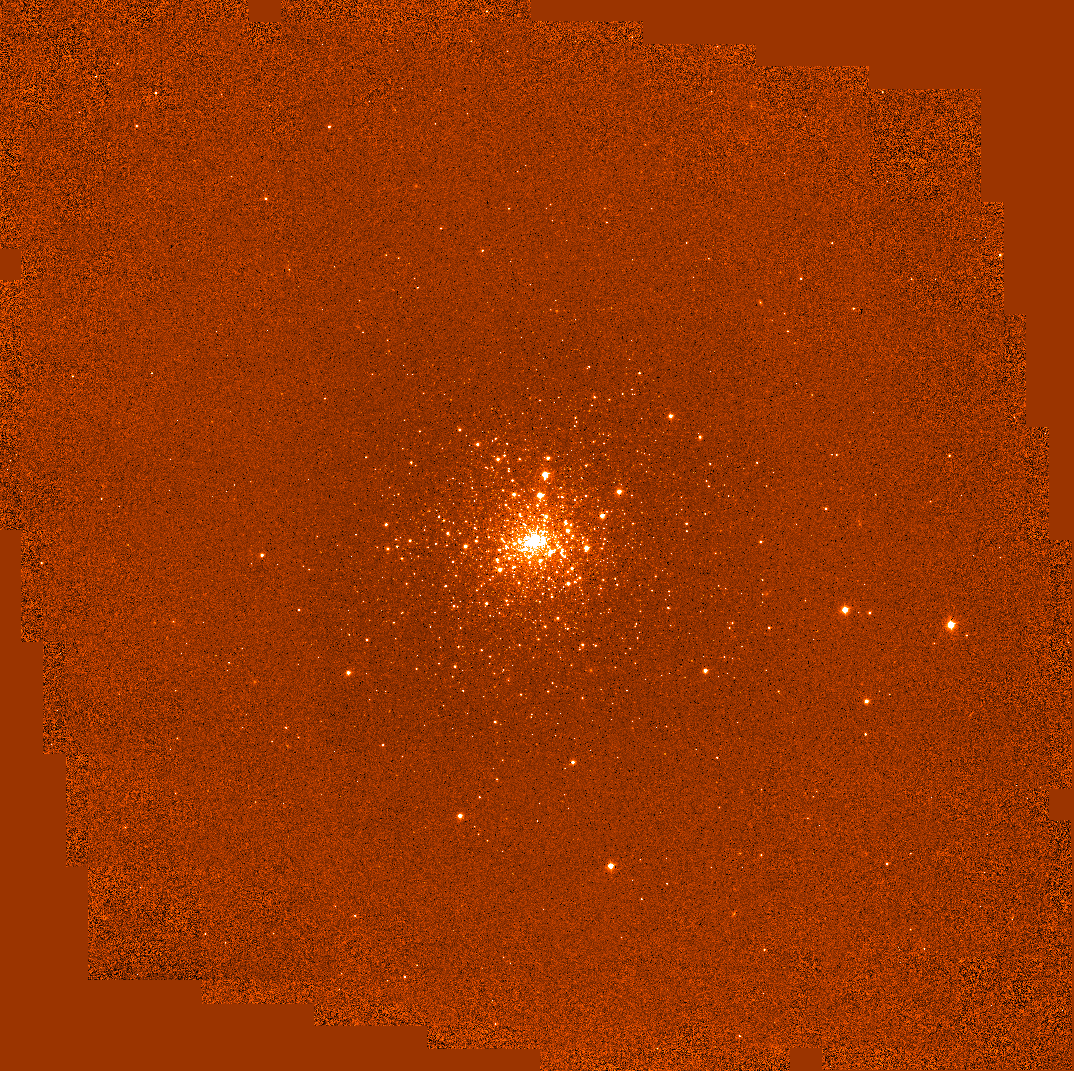
\includegraphics[width=8.4cm]{figures/hdrldemo_resample_DRIZZLE_HAWKI_M30_1.png} 
\caption[]
	{\footnotesize  The final tile image made from 100 HAWK-I images of the M30 field:\\
	{\bf left panel:}    as creating by the HAWK-I pipeline v. 2.4.6 routine {\tt hawki\_science\_postprocess}\\
	{\bf right panel:} as resampled and combined using \hdrlresample\ with {\tt --method=DRIZZLE} and {\tt --method.loop-distance=1}.\\
	}
	\label{fig:hawki_M30}
\end{figure}


As in the previous HAWK-I example, all five methods of image resampling retained the astrometric quality following interpolation.  This is evident in 
figure \ref{fig:radec_M30}.  Here, the absolute positions of the sources in the 100 input HAWK-I images is compared to the absolute positions
of the sources in the image resample using the {\tt QUADRATIC} method.   Here, the median $\Delta\alpha*\cos(\delta)=-0.002\pm0.11\ arcsec$ and 
$\Delta\delta=-0.007\pm0.12\ arcsec$ with the cloud of offsets spread symmetrically about the origin.  
Considering that the HAWK-I pixel size is 0.106 pixels/arcsec, the standard deviation of the astrometric accuracy approximately one pixel.

\begin{figure}[H]
\centering
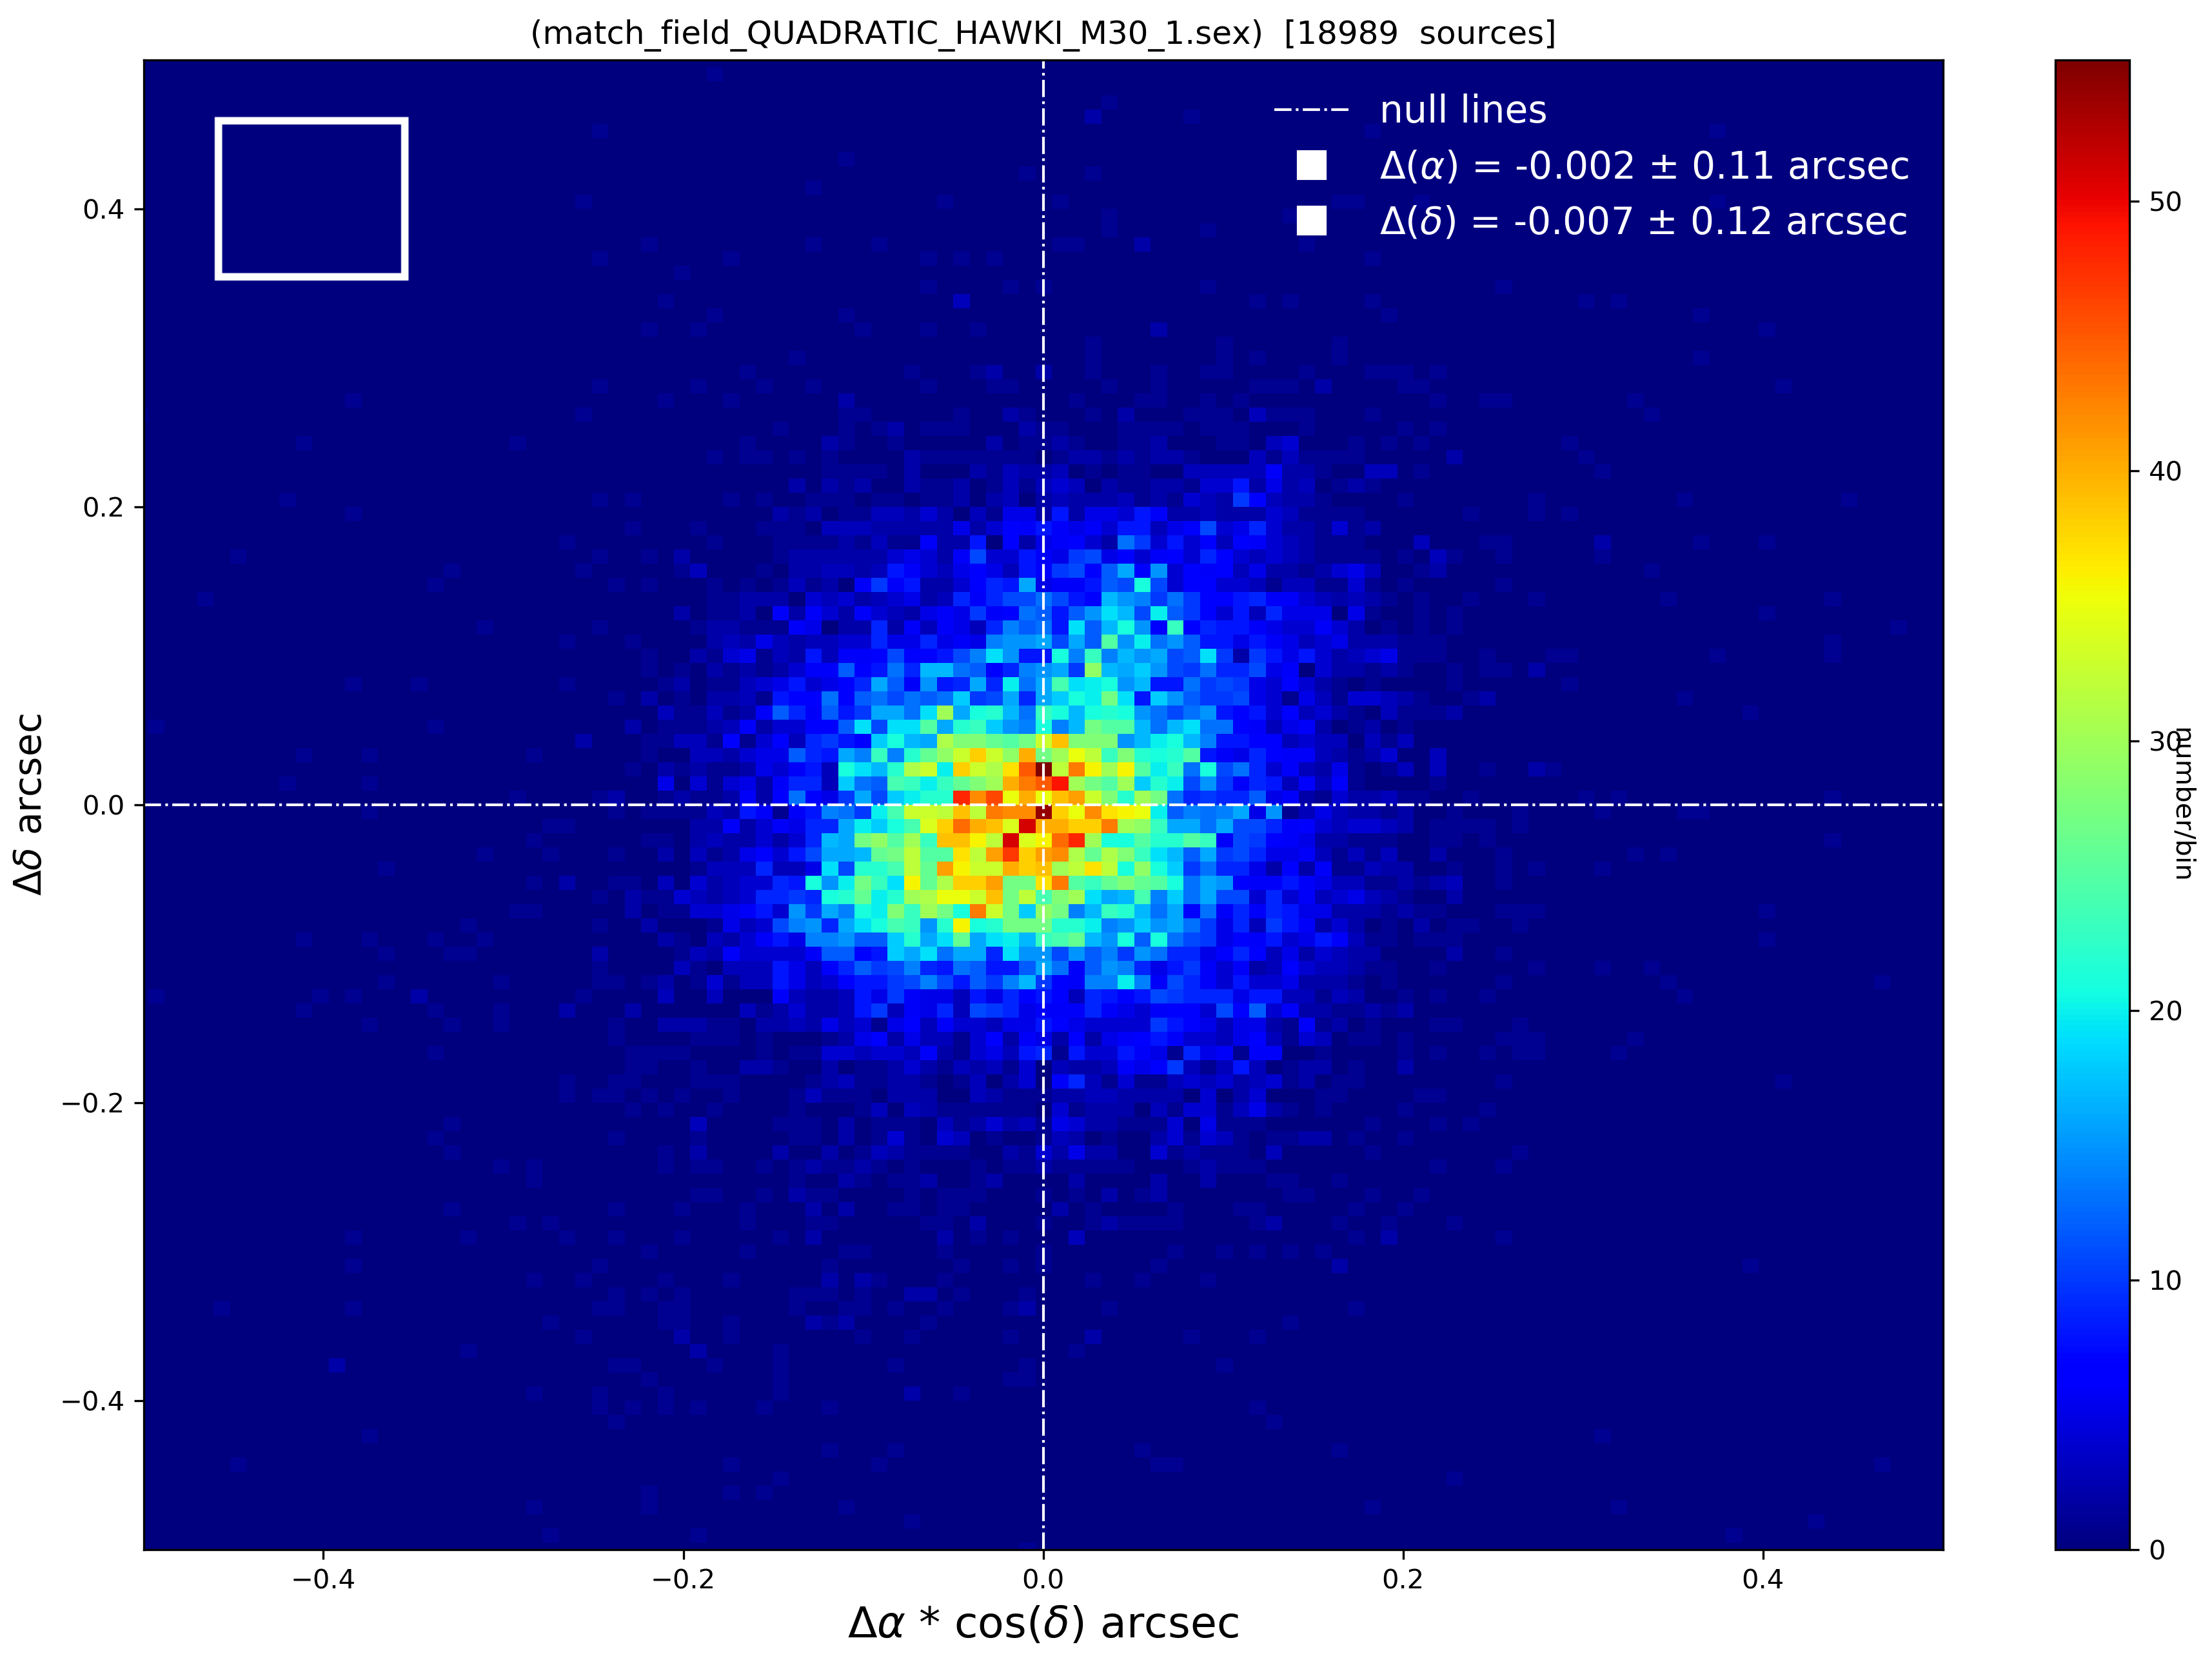
\includegraphics[width=11cm]{figures/match_field_QUADRATIC_HAWKI_M30_1_RA_DEC_scatter_plot.png}
\caption[]
	{\footnotesize  the astrometric quality of the \hdrlresample\ routines as measured by comparing almost 19,000 sources in the original input HAWK-I images
	with those in the resampled ({\tt QUADRATIC}) image tile of Figure \ref{fig:hawki_M30}.
	The standard deviation of the $\Delta\alpha*\cos(\delta)$ and $\Delta\delta$ distributions is 0.12 arcsec. This is approximately the size of one HAWK-I
	pixel (0.106 pixels/arcsec).  The pixel size is indicated by the white square in the top left corner.
	}
	\label{fig:radec_M30}
\end{figure}

Similarly, the photometric quality is also retained following interpolation.   Figure \ref{fig:mag_M30} is typical of all interpolated frames, with a source magnitude match 
between the individual HAWK-I images and the resampled ({\tt LANCZOS}) image tile of $\Delta(mag)=-0.023\pm0.08$ magnitudes.

\begin{figure}[H]
\centering
\includegraphics[width=11cm]{figures/match_field_LANCZOS_HAWKI_M30_1_mag_scatter_plot.png}
\caption[]
	{\footnotesize  the photometric quality of the \hdrlresample\ routines as measured by comparing the more than 18,000 sources in the original input HAWK-I images
	with those in the resampled ({\tt LANCZOS}) image tile of Figure \ref{fig:hawki_M30} (right panel).
	The standard deviation of the $\Delta(mag)$  distribution is 0.08 magnitudes. 	
	}
	\label{fig:mag_M30}
\end{figure}

As can be seen in figure \ref{fig:fwhm_ellip_M30}, the resampling causes a slight increase in the FWHM of the sources and a decrease in the source ellipticities.
This is expected, since the resampling will cause a circularisation and homogenisation of the source shapes.


\begin{figure}[H]
\centering
\includegraphics[width=8.4cm]{figures/match_field_RENKA_HAWKI_M30_3_FWHM_histogram.png}
\includegraphics[width=8.4cm]{figures/match_field_RENKA_HAWKI_M30_3_ellipticity_histogram.png} 
\caption[]
	{\footnotesize  A comparison of FWHM and ellipticity for the sources in the HAWK-I input images (blue histograms) and those
	after resampling (green histograms).  The resampling was done with {\tt --method=RENKA} and {\tt --method.loop-distance=3}.\\
	{\bf left panel:}    The FWHM distribution of the 19,441 sources in the M30 field. As expected, the median FWHM, after resampling, increases slightly.  
	                           Since the increase in FWHM is less than 5\%, this is acceptable.\\
	{\bf right panel:} The distribution of ellipticities.   Here, the resampling has circularised the sources.   This, too, is as expected. 
	}
	\label{fig:fwhm_ellip_M30}
\end{figure}



A summary of the source attributes between the input frames and the resampled images is given in Table \ref{tab:compare_NGC288}.


\begin{sidewaystable}

\caption{A Summary of Comparisons Between Input HAWK-I Cluster Data Images and Resultant Interpolation Images}

\begin{center}
\begin{tabular}{|l|l|c|c|c|c|c|c|c|c|c|c|}                      
\toprule

Image         				     		     & Interpolation	 & N$_{frames}^2$   & Nmatch & $\Delta\alpha$  & $\Delta\delta$ &  $\Delta(mag)$ & $\sigma\Delta(mag)$ & FWHM1$^3$  & FWHM2$^4$  & ellip1$^3$  & ellip2$^4$  \\
                                     & method (LD)$^1$ &                         &               & (arcsec)            & (arcsec)          &                          &                                   & (pixels)    & (pixels)   &            & \\
\midrule
NGC\,288         & DRIZZLE (1)        & 100   	& 10,770 	& 0.001       &  0.003  	& -0.021 & 0.05          & 5.80  	& 6.07		& 0.14    & 0.06   \\
 	   	       	& DRIZZLE (3)        & 100  	& 10,770 	& 0.001       &  0.003  	& -0.021 & 0.05 	  & 5.80  	& 6.07  		& 0.14    & 0.06  \\
 	               	& LANCZOS (1)      & 100  	& 10,768 	& 0.001       &  0.003  	& -0.025 & 0.05          & 5.80  	& 6.01  		& 0.14    & 0.05    \\
 	   	      	& LANCZOS (3)      & 100  	& 10,760 	& 0.000       &  0.003  	& -0.029 & 0.05          & 5.80  	& 5.93  		& 0.14    & 0.05    \\
 	              	& LINEAR (1)          & 100    	& 10,794 	& 0.002       &  0.003  	& -0.012 & 0.05          & 5.80  	& 6.33  		& 0.14    & 0.06    \\
 	              	& LINEAR (3)          & 100    	& 10,782 	& 0.003       &  0.004  	&  0.015 & 0.06          & 5.80  	& 7.56  		& 0.14    & 0.06    \\
 	              	& NEAREST (1)      & 100   	& 9,879 	& -0.001       & 0.002  	& -0.044 & 0.06          & 5.80  	& 5.82  		& 0.13    & 0.12    \\
 	              	& NEAREST (3)      & 100   	& 9,879 	& -0.001       & 0.002  	& -0.044 & 0.06          & 5.80  	& 5.82  		& 0.13    & 0.12    \\
 	              	& QUADRATIC (1)  & 100 	& 10,739 	& 0.001        & 0.004  	& -0.023 & 0.05          & 5.80  	& 6.14  		& 0.14    & 0.06    \\
 	              	& QUADRATIC (3)  & 100 	& 10,724 	& 0.002        & 0.004  	& -0.015 & 0.05          & 5.80  	& 6.52   		& 0.14    & 0.06    \\
 	              	& RENKA (1)           & 100 	& 10,718 	& 0.000        & 0.004  	& -0.030 & 0.05          & 5.80  	& 6.04 		& 0.14    & 0.07    \\
                		& RENKA (3)           & 100  	& 10,718 	& 0.000        & 0.004  	& -0.030 & 0.05          & 5.80  	& 6.04  		& 0.14    & 0.07    \\
\midrule
M\,30         	& DRIZZLE (1)        & 100   	& 18,678 	& -0.002       & -0.006  	& -0.020 & 0.08          & 5.51    & 5.53  		& 0.19    & 0.14    \\
 	   	       	& DRIZZLE (3)        & 100  	& 18,678 	& -0.002       & -0.006  	& -0.020 & 0.08 	 & 5.51    & 5.53  		& 0.19    & 0.14  \\
 	               	& LANCZOS (1)      & 100  	& 18,752 	& -0.002       & -0.007  	& -0.023 & 0.08          & 5.51    & 5.49  		& 0.19    & 0.14    \\
 	   	      	& LANCZOS (3)      & 100  	& 18,852 	& -0.002       & -0.006  	& -0.026 & 0.08          & 5.51    & 5.42  		& 0.19    & 0.14    \\
 	              	& LINEAR (1)          & 100    	& 18,187 	& -0.002       & -0.005  	& -0.008 & 0.09          & 5.50    & 5.77  		& 0.19    & 0.13    \\
 	              	& LINEAR (3)          & 100    	& 16,999 	& -0.001       & -0.004 	&  0.025 & 0.09          & 5.50    & 6.97 		& 0.19    & 0.13    \\
 	              	& NEAREST (1)      & 100   	& 19,189 	& -0.006       & -0.004 	& -0.052 & 0.11          & 5.59    & 5.75  		& 0.20    & 0.21    \\
 	              	& NEAREST (3)      & 100   	& 19,189 	& -0.006       & -0.004  	& -0.052 & 0.11          & 5.59    & 5.75  		& 0.20    & 0.21    \\
 	              	& QUADRATIC (1)  & 100 	& 18,989 	& -0.002       & -0.007  	& -0.026 & 0.09          & 5.52    & 5.66  		& 0.19    & 0.14    \\
 	              	& QUADRATIC (3)  & 100 	& 18,499 	& -0.003       & -0.005  	& -0.016 & 0.09          & 5.51    & 5.97   		& 0.19    & 0.13     \\
 	              	& RENKA (1)           & 100 	& 19,413 	& -0.003       & -0.007  	& -0.034 & 0.09          & 5.53    & 5.63 		& 0.20    & 0.15    \\
                		& RENKA (3)           & 100  	& 19,441 	& -0.003       & -0.007  	& -0.034 & 0.09          & 5.53    & 5.63  		& 0.20    & 0.15    \\
\bottomrule


\end{tabular}	
\end{center}																											

\label{tab:compare_NGC288}
\noindent{
		$^1$ The interpolation method and loop-distance used ({\tt --method.loop-distance}).\\
		$^2$ The total number of synthetic input images combined during the resampling.\\
		$^3$ FWHM1 and ellip1 refer to the individual, HAWK-I input images.\\
		$^4$ FWHM2 and ellip2 refer to the resampled images.}
	\end{sidewaystable}




  
\subsection{Results from Strongly Rotated HAWK-I Images}
\label{sect:hawki2}

In order to test for any flexure in the HAWK-I instrument, an observing block (OB) was designed that allows the camera co-rotator to
travel through 160$^\circ$ while pointing at the same field of view.   This data set was obtained on the night of 2015-08-28 and has
programme id {\tt 60.A-9283(A)} and the observing block id {\tt 200346422}.  It consists of 20 separate exposures of four detectors, with each
pair of images rotated by 20$^\circ$ for a total of 160$^\circ$.   Clearly, a complex data set consisting of 80 distinct detector frames with such
a large overall rotation is an ideal stress test in order to see how well the \hdrlresample\ routines perform.
 
 \begin{figure}[ht]
\centering
\includegraphics[width=8.4cm]{figures/Flexure_M30_TILED_IMAGE.png}
\includegraphics[width=8.4cm]{figures/hdrldemo_resample_DRIZZLE_HAWKI_rotation_1.png} 
\caption[]
	{\footnotesize  The final tile image made from 80 HAWK-I flexure frames:\\
	{\bf left panel:}    Creating by the HAWK-I pipeline v. 2.4.6 routine {\tt hawki\_science\_postprocess}\\
	{\bf right panel:} Resampled and combined using \hdrlresample\ with {\tt --method=DRIZZLE} and {\tt --method.loop-distance=1}.\\
	The only major difference between the two images is that the HAWK-I pipeline trims the tile, whereas \hdrlresample\ creates the a maximal
	area occupied by the WCS from all input images.
	}
	\label{fig:hawki_flexure}
\end{figure}

The 20 $\times$ 4 separate exposures were resampled using each of the methods available in \hdrlresample, {\tt NEAREST, LINEAR, QUADRATIC, RENKA, LANCZOS,
and DRIZZLE}, each with a loop distance of 1 and 3 pixels.   The resulting image tiles were then compared to the tile resulting from processing the identical
data with the HAWK-I pipeline version 2.4.6.

As in the previous HAWK-I example, all five methods of image resampling retained the astrometric quality following interpolation.  This is evident in 
figure \ref{fig:radec_flexure}.  Here, the absolute positions of the sources in the 80 input HAWK-I images is compared to the absolute positions
of the sources in the image resample using the {\tt LINEAR} method.   Here, the median $\Delta\alpha*\cos(\delta)=-0.004\pm0.13\ arcsec$ and 
$\Delta\delta=-0.011\pm0.14\ arcsec$ with the cloud of offsets spread symmetrically about the origin.  
Considering that the HAWK-I pixel size is 0.106 pixels/arcsec, the standard deviation of the astrometric accuracy approximately one pixel.

\begin{figure}[H]
\centering
\includegraphics[width=11cm]{figures/match_field_LINEAR_HAWKI_rotation_1_RA_DEC_scatter_plot.png}
\caption[]
	{\footnotesize  the astrometric quality of the \hdrlresample\ routines as measured by comparing 9,753 sources in the original input HAWK-I images
	with those in the resampled ({\tt LINEAR}) image tile of Figure \ref{fig:hawki_flexure}.
	The standard deviation of the $\Delta\alpha*\cos(\delta)$ and $\Delta\delta$ distributions is 0.14 arcsec. This is approximately the size of one HAWK-I
	pixel (0.106 pixels/arcsec).  The pixel size is indicated by the white square in the top left corner.
	}
	\label{fig:radec_flexure}
\end{figure}

Similarly, the photometric quality is also retained following interpolation.   Figure \ref{fig:mag_flexure} is typical of all interpolated frames, with a source magnitude match 
between the individual HAWK-I images and the resampled ({\tt LINEAR}) image tile of $\Delta(mag)=-0.18\pm0.13$ magnitudes.

\begin{figure}[H]
\centering
\includegraphics[width=11cm]{figures/match_field_LINEAR_HAWKI_rotation_3_mag_scatter_plot.png}
\caption[]
	{\footnotesize  the photometric quality of the \hdrlresample\ routines as measured by comparing the 9,685 sources in the original input HAWK-I images
	with those in the resampled ({\tt LINEAR}) image tile of Figure \ref{fig:hawki_flexure} (right panel).
	The standard deviation of the $\Delta(mag)$  distribution is 0.13 magnitudes. 	
	}
	\label{fig:mag_flexure}
\end{figure}

As can be seen in figure \ref{fig:fwhm_ellip_flexure}, the resampling causes a slight increase in the FWHM of the sources and a decrease in the source ellipticities.
This is expected, since the resampling will cause a circularisation and homogenisation of the source shapes.


\begin{figure}[H]
\centering
\includegraphics[width=8.4cm]{figures/match_field_DRIZZLE_HAWKI_rotation_1_FWHM_histogram.png}
\includegraphics[width=8.4cm]{figures/match_field_DRIZZLE_HAWKI_rotation_1_ellipticity_histogram.png} 
\caption[]
	{\footnotesize  A comparison of FWHM and ellipticity for the sources in the HAWK-I input images (blue histograms) and those
	after resampling (green histograms).  The resampling was done with {\tt --method=DRIZZLE} and {\tt --method.loop-distance=1}.\\
	{\bf left panel:}    The FWHM distribution of the 9,666 sources in the flexure field.  The median FWHM, after resampling, decreases slightly.  
	                           However, this is certainly an artifact of the very broad, ill-defined distribution determined for the input HAWK-I images, being over-estimated.\\
	{\bf right panel:} The distribution of ellipticities.   Here, the resampling has circularised the sources.   This, too, is as expected. 
	}
	\label{fig:fwhm_ellip_flexure}
\end{figure}





A summary of the source attributes between the input frames and the resampled images is given in Table \ref{tab:compare_rotation}.


\begin{sidewaystable}

\caption{A Summary of Comparisons Between Input HAWK-I Flexure Images and Resultant Interpolation Images}

\begin{center}
\begin{tabular}{|l|l|c|c|c|c|c|c|c|c|c|c|}                      
\toprule

Image         				     		     & Interpolation	 & N$_{frames}^2$   & Nmatch & $\Delta\alpha$  & $\Delta\delta$ &  $\Delta(mag)$ & $\sigma\Delta(mag)$ & FWHM1$^3$  & FWHM2$^4$  & ellip1$^3$  & ellip2$^4$  \\
                                     & method (LD)$^1$ &                         &               & (arcsec)            & (arcsec)          &                          &                                   & (pixels)    & (pixels)   &            & \\
\midrule
HAWK-I            & DRIZZLE (1)        & 80    	& 9,666 	& -0.003       & -0.010  	& -0.23 & 0.12          & 7.54  & 7.40  		& 0.16  & 0.07     \\
flexure 	   	& DRIZZLE (3)        & 80    	& 9,666 	& -0.003       & -0.010  	& -0.23 & 0.12 	  	& 7.54  & 7.40  		& 0.16  & 0.07  \\
 	               	& LANCZOS (1)      & 80    	& 9,675 	& -0.003       & -0.009  	& -0.23 & 0.12          & 7.54  & 7.36  		& 0.16  & 0.07   \\
 	   	      	& LANCZOS (3)      & 80    	& 9,657 	& -0.003       & -0.009  	& -0.23 & 0.12          & 7.54  & 7.30  		& 0.16  & 0.07     \\
 	              	& LINEAR (1)          & 80      	& 9,753 	& -0.004       & -0.011  	& -0.21 & 0.12          & 7.54  & 7.61  		& 0.16  & 0.09     \\
 	              	& LINEAR (3)          & 80      	& 9,685 	& -0.004       & -0.013  	& -0.18 & 0.13          & 7.54  & 8.66  		& 0.16  & 0.11     \\
 	              	& NEAREST (1)      & 80     	& 7,788 	& -0.001       & 0.004  	& -0.26 & 0.13          & 7.54  & 7.79  		& 0.16  & 0.14     \\
 	              	& NEAREST (3)      & 80     	& 7,788 	& -0.001       & 0.004  	& -0.26 & 0.13          & 7.54  & 7.79  		& 0.16  & 0.14     \\
 	              	& QUADRATIC (1)  & 80   	& 9,444 	& -0.003       & -0.008  	& -0.22 & 0.13         & 7.54  & 7.75  		& 0.16  & 0.08     \\
 	              	& QUADRATIC (3)  & 80   	& 9,470 	& -0.004       & -0.010  	& -0.21 & 0.13          & 7.54  & 8.00   		& 0.16  & 0.08     \\
 	              	& RENKA (1)           & 80   	& 9,387 	& -0.004       & -0.007  	& -0.24 & 0.12         & 7.54  & 7.72 		& 0.16  & 0.08     \\
                		& RENKA (3)           & 80    	& 9,387 	& -0.004       & -0.007  	& -0.24 & 0.12          & 7.54  & 7.72  		& 0.16  & 0.08     \\
\bottomrule


\end{tabular}	
\end{center}																											

\label{tab:compare_rotation}
\noindent{
		$^1$ The interpolation method and loop-distance used ({\tt --method.loop-distance}).\\
		$^2$ The total number of single, HAWK-I input images combined during the resampling.\\
		$^3$ FWHM1 and ellip1 refer to the original, HAWK-I input images.\\
		$^4$ FWHM2 and ellip2 refer to the resampled images.}
\end{sidewaystable}



\subsection{The Propagation of Edge Effects with Resampled Images}

Astronomical detectors often have edge effects in which the outermost regions of the detector show strongly depressed flux levels.
This can be due to a non-uniform illumination over the surface of the detector, or due to masked edges.   This is particularly evident
in some near infrared detectors.

An edge effect will be strongly enhanced by any resampling method as the algorithm interpolates across such an illumination
discontinuity.   This can be seen in figure \ref{fig:hawki_edges}.  Here, the images of M30 were resampled without first trimming their
edges.  This image should be compared to the right hand panel of figure \ref{fig:hawki_M30}.

The \hdrlresample\ suite will need to include a parameter that allows for the input images to be edge trimmed before
being resampled and combined.  The parameter should be defined as {\tt --edge-trim=NN}, whereby {\tt NN} sets the number of pixels
trimmed from each of the four sides of each input image.
This parameter has already been implemented in the HDRL pipeline kits from version 15 ({\it hdrldemo-kit-1.3.0-15}).

\begin{figure}[H]
\centering
\includegraphics[width=8.4cm]{figures/hdrldemo_resample_DRIZZLE_HAWKI_M30_3.png}
\caption[]
	{\footnotesize  An example of strong edge effects in the final tile image made from 100 HAWK-I images of the M30 field.
	This image has been resampled and combined using \hdrlresample\ with {\tt --method=DRIZZLE} and {\tt --method.loop-distance=1}, 
	without trimming the discontinuities at the edge of each input HAWK-I image.\\
	}
	\label{fig:hawki_edges}
\end{figure}




\subsection{Results from Synthetic Images With Right Ascension values At the Meridian and Declination near the Poles}

A potential pitfall can occur when images straddle discontinuities in the WCS coordinate system.  Therefore, a series of 10 dithered synthetic images were created
with a central pixel values set to reference points:\\
({\tt CRVAL1, CRVAL2}) = $(\alpha_{\circ}, \delta_{\circ})$ = (360$^\circ$, 88$^\circ$). \\
These synthetic images were then resampled and combined using the six available \hdrlresample\ methods.   In each case, the resampled frames correctly retain the
celestial coordinates of the original input images.   This can seen in figure \ref{fig:discontinuity}, in which the ds9 coordinate grid is overlaid on the images and displays
the correct transition straddling the $0^\circ$ meridian.


\begin{figure}[H]
\centering
\includegraphics[width=8.1cm]{figures/synth_disc2_stars_gal_bkgd_1.png}
\includegraphics[width=8.6cm]{figures/hdrldemo_resample_DRIZZLE_disc2_coadd_1.png} 
\caption[]
	{\footnotesize  A synthetic image and its resampled counterpart to test the \hdrlresample\ routines at and near celestial discontinuities  \\
	{\bf left panel:}    A single synthetic frame with {\tt (CRVAL1, CRVAL2)} =  $(\alpha, \delta) = 360^\circ, -88^\circ$).      \\
	{\bf right panel:}  The ten synthetic resampled and combined using \hdrlresample\ with {\tt --method=DRIZZLE} and {\tt --method.loop-distance=1}.\\
	The overlaid ds9 coordinate grid shows that these extreme $(\alpha, \delta)$ values are handled correctly.
	}
	\label{fig:discontinuity}
\end{figure}



\subsection{Testing the \hdrlresample\ Routines Using MUSE Data Cubes}

Tests on MUSE datacubes were performed on dithered observations of two
targets: TNJ2009-304 (a protocluster at z$\sim$3) and FCC 184 (an
early-type galaxy in the Fornax cluster).

The cube of TNJ2009-304 includes the combination of 6 dithered
exposures (MUSE.2016-06-01T06:09:25.499.fits,
MUSE.2016-06-01T07:05:35.072.fits, MUSE.2016-06-01T08:24:39.641.fits,
MUSE.2016-06-01T09:19:35.838.fits, MUSE.2016-06-08T06:06:02.858.fits,
and MUSE.2016-06-08T06:58:50.486.fits).

 The cube of GCC 184 includes
the combination of 10 dithered exposures
(MUSE.2017-01-26T02:57:56.013.fits, MUSE.2017-01-26T03:16:12.338.fits,
MUSE.2017-01-26T03:30:08.819.fits, MUSE.2017-01-26T03:49:23.358.fits,
MUSE.2017-01-26T04:03:20.921.fits, MUSE.2017-11-15T06:57:38.494.fits,
MUSE.2017-11-15T07:15:56.735.fits, MUSE.2017-11-15T07:29:49.482.fits,
MUSE.2017-11-15T07:48:08.059.fits, and
MUSE.2017-11-15T08:02:02.941.fits).


First, the data were reduced and combined with the MUSE pipeline
(v2.8.3). This process foresees the combination of so-called
pixel-tables, each of them represent the fully reduced exposure in
detector space. The direct combination of pixel tables implies one
single regridding process of the data.


The MUSE pipeline also produced the regridded cubes of the individual
exposures, which we then combined (after taking into account spatial
offsets in RA/DEC) with the HDRL recipe \hdrlresample. This process
implies two regriddings: the first is done by the MUSE pipeline to
``convert'' each pixel table into a datacube. The second is done by
HDRL to regrid each cube into a common WCS before combining them.

The combination was done using the same parameters as in MUSE; drizzle
method with downscaling factor 0.6 (spatial and spectral dimension),
and loop-distance =1 pixel. The variance extension in the MUSE
individual datacubes was also used.

Also, we set the starting and ending RA/DEC in the HDRL recipe so that
the final cube spatially matches the MUSE combined cube.  In this way a
direct 1-to-1 spaxel comparison is possible.

The goals are to compare the quality of the spatial resolution and
spectra obtained with two approaches; a direct combination of reduced
pixel-tables with the MUSE pipeline, and the combination of individual
pre-regridded cubes with HDRL.


\subsubsection{Spatial resolution}

Figure \ref{fig:muse_hdrl_fov} compares the white-lamp images obtained
by collapsing the MUSE and HDRL datacubes along the wavelength
axis. The HDRL cubes are smoother in the spatial direction, as a
consequence of the two-regridding steps that are involved in the
process. Table \ref{tab:compare_psf_muse} compares the MOFFAT point
spread function (measured with IRAF) of point-like sources measured on
the reconstructed images. On average, the HDRL cubes have FWHM 1-2\%
higher than the corresponding source in the MUSE cube.

 
\begin{table}
\caption{Point spread function of point-like sources in the reconstructed field of views}
\begin{center}
\begin{tabular}{l c c c c c c}
 ID &  X   &     Y  &     RA    &  DEC        &   MOFFAT\_MUSE& MOFFAT\_HDRL \\
    &  pxl &   pxl  & [$^\circ$] &  [$^\circ$]  &   pxl   &    pxl \\
\hline
    &      &        &           &  TNJ2009-304  &         &         \\
1   &40.48 & 285.49 &302.4580383 &--30.6613064 &  4.73   &  4.75   \\ 
2   &97.99 & 190.29 &302.4543457 &--30.6665955 &  4.49   &  4.56   \\
3   &168.09&  214.34& 302.4497986& --30.6652584&   4.53  &   4.61  \\
4   &262.61&  215.91& 302.4436951& --30.6651707&   5.78  &   5.85  \\
5   &254.20&  189.76& 302.4442444& --30.6666241&   4.30  &   4.41  \\
6   &155.89&  143.03& 302.4505920& --30.6692200&   4.78  &   4.82  \\
    &      &        &            &   FCC184    &         &         \\
7   &194.40&  355.39&  54.2386971& --35.4991646&   4.50  &    4.59 \\ 
\hline
\end{tabular}	
\end{center}																				
\label{tab:compare_psf_muse}
\end{table}




\begin{figure}[H]
\centering
\includegraphics[width=17cm]{figures/fovs.jpg}
\includegraphics[width=17cm]{figures/fovs2.jpg}
\caption[] {\footnotesize Comparison between the reconstructed fields
  of view obtained by combining individual reduced pixel tables with
  the MUSE pipeline (left) and by combining individual reduced cubes
  with hdrl\_demo\_resample (right). The figure on the top refers to
  TNJ2009-304, the figure on the bottom to FCC 184. The numbers
  indicate the sources we measured the Moffat PSF in Table
  \ref{tab:compare_psf_muse}. The letters indicate the sources we
  compare in the spectra of figures \ref{fig:muse_hdrl_spaxel} to
  \ref{fig:muse_hdrl_profile}. }
	\label{fig:muse_hdrl_fov}
\end{figure}


\subsubsection{Difference in spectra}

In this section we quantify the differences in the spectral properties
due to the different resampling scheme. The analysis is done for the 3
sources in the field of TNJ2009-304, marked as A, B, and C in Figure
\ref{fig:muse_hdrl_fov}.

The first effect of the smearing in the spatial resolution is that in
the HDRL cube the flux is distributed on a larger area than in the
MUSE cube. Therefore, at each spaxel the flux level is different; in
the studied sources this difference can be as large as 5\% (see figure
\ref{fig:muse_hdrl_spaxel}), but it obviously depends on the spatial
profile, the difference being larger for more peaked profiles.

We then measured the changes in the integrated flux of individual
sources; we compared the flux of some sources integrated on a 5x5 box
around the source peak.  This comparison is shown in figures
\ref{fig:muse_hdrl_spcA}--\ref{fig:muse_hdrl_spcC}.

As shown in these figures, there are small difference between spectra
of the same source extracted from the MUSE and HDRL datacubes, of the
order of 1-2\%. The S/N ratio of the spectra extracted from the cube
produced by HDRL is a few percent higher than the S/N of spectra
extracted from datacubes combined with the MUSE pipeline; this is
expected, as the two regridding process also smooths the spectra along
the wavelength direction.

Figure \ref{fig:muse_hdrl_profile} shows the comparison between the
spectra of source A on a wavelength region around prominent absorption
lines (CaT). The figure shows that, while the continuum of the two
spectra is more or less the same (a small offset $<0.5$\% is visible),
the shape of the absorption lines differ by $\approx 1$\%. This means
that the combination of datacubes (that implies 2 resamplings) can
``damage'' the shape of line features by $\approx $1\% with respect to
the combination of reduced pixel tables.




\begin{figure}[H]
\centering
\includegraphics[width=12cm]{figures/spc_A_single_spaxel.jpg}
\caption[] {\footnotesize Top panel. Comparison between the central spaxel
  of source A shown in \ref{fig:muse_hdrl_fov} in the cube obtained by
  combining individual reduced pixel tables with the MUSE pipeline
  (left orange) and the one obtained by combining individual reduced
  cubes with hdrl\_demo\_resample (blue). Bottom panel, the difference
  in percentage between the 2 spectra of the top panel. }
	\label{fig:muse_hdrl_spaxel}
\end{figure}


\begin{figure}[H]
\centering
\includegraphics[width=12cm]{figures/spc_A.jpg}
\caption[] {\footnotesize Top panel. Comparison between the spectrum
  of source A shown in \ref{fig:muse_hdrl_fov} in the cube obtained by
  combining individual reduced pixel tables with the MUSE pipeline
  (left orange) and the one obtained by combining individual reduced
  cubes with hdrl\_demo\_resample (blue). The spectrum is obtained by
  integrating a 7x7 box around the spaxel indicated in the
  image. Bottom panel, the difference in percentage between the 2
  spectra of the top panel.}
	\label{fig:muse_hdrl_spcA}
\end{figure}


\begin{figure}[H]
\centering
\includegraphics[width=12cm]{figures/spc_B.jpg}
\caption[] {\footnotesize As in figure \ref{fig:muse_hdrl_spcA}, but for source B in figure \ref{fig:muse_hdrl_fov}.}
	\label{fig:muse_hdrl_spcB}
\end{figure}

\begin{figure}[H]
\centering
\includegraphics[width=12cm]{figures/spc_C.jpg}
\caption[] {\footnotesize As in figure \ref{fig:muse_hdrl_spcA}, but for source C in figure \ref{fig:muse_hdrl_fov}.}
	\label{fig:muse_hdrl_spcC}
\end{figure}

\begin{figure}[H]
\centering
\includegraphics[width=12cm]{figures/line_shape.jpg}
\caption[] {\footnotesize As in figure \ref{fig:muse_hdrl_spcA}, but for the wavelength region around CaT absorption features.}
	\label{fig:muse_hdrl_profile}
\end{figure}


\subsubsection{Difference in derived properties}

In this section we measure the differences in physical properties
derived from the analysis of the spectra extracted from the MUSE and
HDRL cubes. As example, we study the two-dimensional velocity field of
the ionized gas in FCC 184. The galaxy is known to have a steep
spatial gradient of the rotational velocity. We aim at quantifying how
much the velocity gradient is affected by the smearing effect.

The analysis is done for the cube of FCC 184.

In each spaxel we fit H$\alpha$ (6562.82 \AA) and
[N\small{II}](6548.03,6583.41 \AA) emission lines; the 3 lines share
the same radial velocity and velocity dispersion. In the fit, we
include a broad H$\alpha$ in absorption (with independent velocity and
velocity dispersion) and a 5-th order additive polynomium to mimic the
effect of the underlying stellar continuum.

Figure \ref{fig:FCC184_velocity_field} compares the central
two-dimensional velocity fields obtained from the MUSE cube and HDRL
cube. The smearing smooths the velocity field, which is less noisy in
the HDRL cube. The impact of the central velocity gradient is within 1
sigma, as shown in Figure \ref{fig:FCC184_rotation_velocity}. In the
velocity field extracted from the MUSE cube, the velocity gradient is
$\sim 9.84 \pm 0.40$ km/sec/arcsec (measured along PA
$ \sim 55^{\circ}$). In the velocity field extracted from the HDRL
cube, the velocity gradient is a bit shallower, and it amounts to
$9.36 \pm 0.24$ km/sec/arcsec.




\begin{figure}[H]
\centering
\includegraphics[width=16cm]{figures/FCC184_velocity_field.jpeg}
\caption[] {\footnotesize Comparison between the two-dimensional velocity fields of
  FCC 184 as measured in the MUSE cube (left) and right cube
  (HDRL). The velocity range is from 1220 to 1360 km/sec}
\label{fig:FCC184_velocity_field}
\end{figure}

\begin{figure}[H]
\centering
\includegraphics[width=16cm]{figures/FCC184_rotation_velocity.jpeg}
\caption[] {\footnotesize Comparison between the rotation curves extracted from the
  velocity fields (PA $\sim 55^{\circ}$). The central velocity
  gradient is measured from the central 6 pixels (1 pixel = 1.25
  arcsec), and it amounts to $12.3 \pm 0.5$ km/sec/pixel
  ($\sim 9.84 \pm 0.40$ km/sec/arcsec) for the MUSE velocity field and
  $11.7 \pm 0.3$ km/sec/pixel ($9.36 \pm 0.24$ km/sec/arcsec) for the
  HDRL velocity field.}
\label{fig:FCC184_rotation_velocity}
\end{figure}


\subsection{Error Handling in \hdrlresample}
\label{sect:errors}

The routines within \hdrlresample\ allow for the propagation of errors.   To test whether or not the errors are propagated correctly,
a number of synthetic error data sets have been created.   The first set consists of a single and 10 dithered synthetic images with
Gaussian-like errors.   The second set consists of a single and 30 dithered synthetic images with a constant error of 10 e$^-$.

\subsubsection{Gaussian Errors}
The background of each synthetic image was created using the {\tt iraf.mknoise} function with a background level of 500 e$^-$.
with Poisson noise, a gain of 2.5 e$^{-}$/ADU, and a Gaussian readnoise of 5.0 e$^{-}$.   This resulted in synthetic images with a
background of 500 $\pm$ 19.3 e$^-$.   
% std_dev = 55.5
% trim_std_dev = 19.3
% iraf_std = 12.5
A faux error plane was then created by simply taking the square root of the data signal.   This resulted in a synthetic error plane
with an average level of 11.2 $\pm$ 0.3 e$^-$.
% std_dev = 0.59
% trim_std_dev = 0.301
% iraf_std = 0.219

Based on this, we would expect the median error plane of the resampled images with a single synthetic image as input to
be close to the 11.2 $\pm$ 0.3 e$^-$ value.   As can be seen in table \ref{tab:errors}, this is the case for all interpolation methods
except for the {\tt LINEAR} method.  Clearly, the {\tt LINEAR} method is significantly underestimating the error.

For the resampled combination of 10 synthetic images, the error propagation should deliver an average error value of approximately 
$\frac{11.2}{\sqrt{10}}$ = 3.5 e$^-$.  It would appear from table \ref{tab:errors} that the {\tt NEAREST} method significantly over-estimates the error.
However, since the {\tt NEAREST} method takes the nearest value of each pixel in both the area around it, and in the stack of combined frames.
Thus, the {\tt NEAREST} method does not compute a strict average of combined frames, this error value is correct.

%
% For loop-distance=1 ==> 1 pixels goes to 9 pixels.     $\frac{11.2}{\sqrt{10}}/\sqrt{9}$   = 1.18  e$^-$.
% For loop-distance=3 ==> 1 pixels goes to 49 pixels.   $\frac{11.2}{\sqrt{10}}/\sqrt{49}$ = 0.51 e$^-$.
%



\begin{table}
\caption{Error Statistics of the Synthetic Data Images (Normal Errors) and the Resultant Interpolation Images}
\begin{center}
\begin{tabular}{|l|c|c|c|}
\toprule

         Image[ext]$^1$                                       &median              &trim\_mean         &trim\_std\_dev       \\ 
\midrule
         synthetic\_stars\_gal\_bkgd\_1$\ldots$10.fits[2]               &11.199              &11.202              &0.305         \\
\midrule
         hdrldemo\_resample\_DRIZZLE\_single\_1.fits[3]       &11.165              &11.151              &0.464         \\
         hdrldemo\_resample\_DRIZZLE\_single\_3.fits[3]       &11.165              &11.151              &0.464         \\
         hdrldemo\_resample\_LANCZOS\_single\_1.fits[3]       &11.134              &11.121              &3.278         \\
         hdrldemo\_resample\_LANCZOS\_single\_3.fits[3]       &11.146              &11.135              &3.180         \\
         hdrldemo\_resample\_LINEAR\_single\_1.fits[3]        &8.969  			&8.958  &0.395         \\
         hdrldemo\_resample\_LINEAR\_single\_3.fits[3]        &6.381  			&6.374  &0.401         \\
         hdrldemo\_resample\_NEAREST\_single\_1.fits[3]       &11.165              &11.151              &0.464         \\
         hdrldemo\_resample\_NEAREST\_single\_3.fits[3]       &11.165              &11.151              &0.464         \\
         hdrldemo\_resample\_QUADRATIC\_single\_1.fits[3]     &11.076              &11.062              &0.514         \\
         hdrldemo\_resample\_QUADRATIC\_single\_3.fits[3]     &11.000              &10.986              &0.818         \\
         hdrldemo\_resample\_RENKA\_single\_1.fits[3]         &11.143              &11.129              &0.488         \\
         hdrldemo\_resample\_RENKA\_single\_3.fits[3]         &11.144              &11.131              &0.487         \\
\midrule 
         hdrldemo\_resample\_DRIZZLE\_coadd\_1.fits[3]        &2.503		   &2.544               &0.900         \\
         hdrldemo\_resample\_DRIZZLE\_coadd\_3.fits[3]        &2.503               &2.544               &0.900         \\
         hdrldemo\_resample\_LANCZOS\_coadd\_1.fits[3]        &2.653               &2.699               &0.961         \\
         hdrldemo\_resample\_LANCZOS\_coadd\_3.fits[3]        &2.926               &2.983               &1.110         \\
         hdrldemo\_resample\_LINEAR\_coadd\_1.fits[3]         &1.323               &1.346               &0.502         \\
         hdrldemo\_resample\_LINEAR\_coadd\_3.fits[3]         &0.632               &0.645               &0.240         \\
         hdrldemo\_resample\_NEAREST\_coadd\_1.fits[3]        &11.162 	   &11.148 		&0.450         \\
         hdrldemo\_resample\_NEAREST\_coadd\_3.fits[3]        &11.162          &11.148 			&0.450         \\
         hdrldemo\_resample\_QUADRATIC\_coadd\_1.fits[3]      &1.703               &1.733               &0.624         \\
         hdrldemo\_resample\_QUADRATIC\_coadd\_3.fits[3]      &1.199               &1.222               &0.430         \\
         hdrldemo\_resample\_RENKA\_coadd\_1.fits[3]          &2.149               &2.186               &0.778         \\
         hdrldemo\_resample\_RENKA\_coadd\_3.fits[3]          &2.126               &2.165               &0.776         \\
\bottomrule

\end{tabular}	
\end{center}																											

\label{tab:errors}
\noindent{
		$^1$ The image and the [extension] of the error frame. \\
		}
\end{table}



\subsubsection{Constant Errors}

For this data set,  a faux error plane was then created and set to a constant value of 10 e$^-$. 
Based on this, we would expect the error plane of the resampled images with a single synthetic image as input to
be close to the 10.0 $\pm$ 0.0 e$^-$ value.   As can be seen in table \ref{tab:errors_fixed}, this is the case for all interpolation methods
except for the {\tt LINEAR} method.  Clearly, the {\tt LINEAR} method is again underestimating the error when a single image is being resampled.

For the resampled combination of 30 synthetic images, the error propagation should deliver an average error value of approximately 
$\frac{10.0}{\sqrt{30}}$ = 1.83 e$^-$.  As can be seen in table \ref{tab:errors_fixed}, the {\tt LINEAR} method slightly under-estimates the error.
The same may be true of the {\tt QUADRATIC} method.
It would also appear that the {\tt NEAREST} method significantly over-estimates the error.
However, since the {\tt NEAREST} method takes the nearest value of each pixel in both the area around it, and in the stack of combined frames, this
value is correct.  



\begin{table}[H]
\caption{Error Statistics of the Synthetic Data Images (Fixed Errors) and the Resultant Interpolation Images}
\begin{center}
\begin{tabular}{|l|c|c|c|}
\toprule

         Image[ext]$^1$                                       				&median              &trim\_mean         &trim\_std\_dev       \\ 
\midrule
         synthetic\_stars\_gal\_bkgd\_1$\ldots$30.fits[2]               &10.00              &10.00              &0.00         \\
\midrule
hdrldemo\_resample\_DRIZZLE\_single\_1.fits[3]             & 10.000      & 10.000     & 0.000         \\
hdrldemo\_resample\_DRIZZLE\_single\_3.fits[3]             & 10.000      & 10.000     & 0.000         \\
hdrldemo\_resample\_LANCZOS\_single\_1.fits[3]             & 9.971       & 9.971     & 2.869         \\
hdrldemo\_resample\_LANCZOS\_single\_3.fits[3]             & 9.979       & 9.979      & 2.795         \\
hdrldemo\_resample\_LINEAR\_single\_1.fits[3]              & 8.031      & 8.031      & 0.122         \\
hdrldemo\_resample\_LINEAR\_single\_3.fits[3]              & 5.713       & 5.713      & 0.271         \\
hdrldemo\_resample\_NEAREST\_single\_1.fits[3]             & 10.000      & 10.000     & 0.000         \\
hdrldemo\_resample\_NEAREST\_single\_3.fits[3]             & 10.000      & 10.000     & 0.000         \\
hdrldemo\_resample\_QUADRATIC\_single\_1.fits[3]           & 9.920       & 9.920      & 0.205         \\
hdrldemo\_resample\_QUADRATIC\_single\_3.fits[3]           & 9.852       & 9.852      & 0.605         \\
hdrldemo\_resample\_RENKA\_single\_1.fits[3]               & 9.981       & 9.981      & 0.141         \\
hdrldemo\_resample\_RENKA\_single\_3.fits[3]               & 9.980       & 9.980      & 0.143         \\
\midrule
hdrldemo\_resample\_DRIZZLE\_coadd\_1.fits[3]              & 1.291       & 1.320      & 0.533         \\
hdrldemo\_resample\_DRIZZLE\_coadd\_3.fits[3]              & 1.291       & 1.320      & 0.533         \\
hdrldemo\_resample\_LANCZOS\_coadd\_1.fits[3]              & 1.368       & 1.399      & 0.564         \\
hdrldemo\_resample\_LANCZOS\_coadd\_3.fits[3]              & 1.509       & 1.547      & 0.619         \\
hdrldemo\_resample\_LINEAR\_coadd\_1.fits[3]               & 0.683       & 0.698      & 0.281         \\
hdrldemo\_resample\_LINEAR\_coadd\_3.fits[3]               & 0.326       &0.334      & 0.137         \\
hdrldemo\_resample\_NEAREST\_coadd\_1.fits[3]              & 10.000      & 10.000     & 0.000         \\
hdrldemo\_resample\_NEAREST\_coadd\_3.fits[3]              & 10.000      & 10.000     & 0.000         \\
hdrldemo\_resample\_QUADRATIC\_coadd\_1.fits[3]            & 0.878       & 0.898      & 0.363         \\
hdrldemo\_resample\_QUADRATIC\_coadd\_3.fits[3]            & 0.618       & 0.634     & 0.252         \\
hdrldemo\_resample\_RENKA\_coadd\_1.fits[3]                & 1.108       & 1.133      & 0.457         \\
hdrldemo\_resample\_RENKA\_coadd\_3.fits[3]                & 1.096       & 1.122      & 0.452         \\
\bottomrule

\end{tabular}	
\end{center}																											

\label{tab:errors_fixed}
\noindent{
		$^1$ The image and the [extension] of the error frame. \\
		}
\end{table}




\section{Definition of Limiting Magnitude}
\label{chap:algorithms:maglim}

%\subsection{Detailed Description of the Limiting Magnitude Algorithm}

The Equation 13 of Naylor 1998, MNRAS,296, 339 gives the signal to
noise $Q$ of a source of total flux $T$ that can be reached with
optimal extraction:

\begin{equation}
Q=\frac{T}{FWHM\cdot\Sigma_1}\sqrt{\frac{2\ln(2)}{\pi}}
\end{equation}
$FWHM$ is the full with half maximum of the seeing.
%Gaussian $g$ function I have used to convolve my image.
$\Sigma_1$ is the standard deviation of the background noise ``before'' convolution with the Gaussian.


\begin{equation}
T=\frac{Q \cdot FWHM \cdot \Sigma_1 \pi^{1/2}}{\sqrt{2\ln(2)}}
\end{equation}

Replacing $\sigma =  FWHM/\sqrt{4\ln4}$:
\begin{eqnarray}
T&=&\frac{Q  \sigma\sqrt{4\ln4}  \cdot \Sigma_1 \pi^{1/2}}{\sqrt{2\ln(2)}}\nonumber\\
 &=&\frac{Q  2\sigma\sqrt{2\ln2}  \cdot \Sigma_1 \pi^{1/2}}{\sqrt{2\ln(2)}}\nonumber\\
 &=& Q  2\sigma  \cdot \Sigma_1 \pi^{1/2}
\end{eqnarray}

If I convolve the background by a Gaussian function $g$ with $FWHM$
equal to the seeing, then I obtain another image, with its standard
deviation $\Sigma_2$. If the original background has a Gaussian
distribution with standard deviation $\Sigma_1$, then $\Sigma_1$ is
related to $\Sigma_2$ by:

\begin{equation}
\Sigma_1 = 2 \Sigma_2 \cdot \pi^{1/2} \cdot \sigma
\label{eqn:noise_conv}
\end{equation}

Hence:
\begin{eqnarray}
T&=& Q  2\sigma  \cdot \left( 2\Sigma_2  \cdot \pi^{1/2} \cdot \sigma \right) \pi^{1/2}\nonumber\\
&=& 4 Q  \sigma^2  \cdot \Sigma_2  \cdot \pi 
\end{eqnarray}

The flux $T$ of a source that is $Q=5$ brighter than the noise $N$
defines the limiting magnitude ($Q=T/N$ is the signal to noise):
\begin{eqnarray}
AB_{\rm MAGLIM} &=& -2.5\log\left( 5\cdot N  \right) +Z_{\rm PT}  \nonumber\\
            &=& -2.5\log\left( 5\cdot T \cdot N/T \right)  +Z_{\rm PT}  \nonumber\\
            &=& -2.5\log\left( 5\cdot T/Q \right)  +Z_{\rm PT}  \nonumber\\
            &=& -2.5\log\left( 5Q(4 \Sigma_2 \cdot \pi \sigma^2 )/Q \right)  +Z_{\rm PT} \nonumber\\
            &=& -2.5\log (2\cdot 2\cdot 5 \Sigma_2 \cdot \pi \sigma^2 )  +Z_{\rm PT} \nonumber\\
            &=& -2.5\log ( 5 \Sigma_2 \cdot 2 \pi \sigma^2 ) +Z_{\rm PT} -2.5\log 2
\label{eqn:abmaglim}
\end{eqnarray}
Which is equivalent to (in the case of Gaussian noise):
\begin{eqnarray}
AB_{\rm MAGLIM} &=& -2.5\log \left( 5   \frac{ \Sigma_1}{ 2\pi^{1/2}\sigma} \cdot 2 \pi \sigma^2 \right) +Z_{\rm PT} -2.5\log 2  \nonumber\\
 &=& -2.5\log \left( 5  \Sigma_1 \cdot \pi^{1/2} \sigma \right) +Z_{\rm PT} -2.5\log 2 
\end{eqnarray}

Note. Equation \ref{eqn:noise_conv}  is the solution of the integral.
\begin{eqnarray}
\Sigma_2 (r)&=& \Sigma_1(r)\sqrt{\int_0^{\infty}{ \frac{2\pi r}{(2\sigma^2\pi)^2} \left( e^{\frac{-r^2}{2\sigma^2}} \right)^2  dr} } \nonumber\\
            &=& \Sigma_1(r)\sqrt{\int_0^{\infty}{ 2\pi r \left( \frac{e^{\frac{-r^2}{2\sigma^2}}}{2\sigma^2\pi} \right)^2  dr} } \nonumber\\
            &=& \Sigma_1(r)\sqrt{\int_0^{\infty}{ 2\pi r  g^2(r;\sigma)  dr} } \nonumber\\
\end{eqnarray}

where $r=\sqrt{x^2+y^2}$ represent the radial coordinates and $g(r;\sigma)$ is the Gaussian function used for the convolution.

{\bf HDRL implements equation \ref{eqn:abmaglim}}, see \ref{sec:algorithms:maglim:algo}. It implements image
convolution; this step is indeed needed to include all non-gaussian noise and
features in an image that might affect the computation of the
magnitude.

\begin{center}
  \bf{--- End of document ---}
\end{center}
\end{document}
